% Options for packages loaded elsewhere
% Options for packages loaded elsewhere
\PassOptionsToPackage{unicode}{hyperref}
\PassOptionsToPackage{hyphens}{url}
%
\documentclass[
  letterpaper,
]{scrbook}
\usepackage{xcolor}
\usepackage{amsmath,amssymb}
\setcounter{secnumdepth}{5}
\usepackage{iftex}
\ifPDFTeX
  \usepackage[T1]{fontenc}
  \usepackage[utf8]{inputenc}
  \usepackage{textcomp} % provide euro and other symbols
\else % if luatex or xetex
  \usepackage{unicode-math} % this also loads fontspec
  \defaultfontfeatures{Scale=MatchLowercase}
  \defaultfontfeatures[\rmfamily]{Ligatures=TeX,Scale=1}
\fi
\usepackage{lmodern}
\ifPDFTeX\else
  % xetex/luatex font selection
\fi
% Use upquote if available, for straight quotes in verbatim environments
\IfFileExists{upquote.sty}{\usepackage{upquote}}{}
\IfFileExists{microtype.sty}{% use microtype if available
  \usepackage[]{microtype}
  \UseMicrotypeSet[protrusion]{basicmath} % disable protrusion for tt fonts
}{}
\makeatletter
\@ifundefined{KOMAClassName}{% if non-KOMA class
  \IfFileExists{parskip.sty}{%
    \usepackage{parskip}
  }{% else
    \setlength{\parindent}{0pt}
    \setlength{\parskip}{6pt plus 2pt minus 1pt}}
}{% if KOMA class
  \KOMAoptions{parskip=half}}
\makeatother
% Make \paragraph and \subparagraph free-standing
\makeatletter
\ifx\paragraph\undefined\else
  \let\oldparagraph\paragraph
  \renewcommand{\paragraph}{
    \@ifstar
      \xxxParagraphStar
      \xxxParagraphNoStar
  }
  \newcommand{\xxxParagraphStar}[1]{\oldparagraph*{#1}\mbox{}}
  \newcommand{\xxxParagraphNoStar}[1]{\oldparagraph{#1}\mbox{}}
\fi
\ifx\subparagraph\undefined\else
  \let\oldsubparagraph\subparagraph
  \renewcommand{\subparagraph}{
    \@ifstar
      \xxxSubParagraphStar
      \xxxSubParagraphNoStar
  }
  \newcommand{\xxxSubParagraphStar}[1]{\oldsubparagraph*{#1}\mbox{}}
  \newcommand{\xxxSubParagraphNoStar}[1]{\oldsubparagraph{#1}\mbox{}}
\fi
\makeatother

\usepackage{color}
\usepackage{fancyvrb}
\newcommand{\VerbBar}{|}
\newcommand{\VERB}{\Verb[commandchars=\\\{\}]}
\DefineVerbatimEnvironment{Highlighting}{Verbatim}{commandchars=\\\{\}}
% Add ',fontsize=\small' for more characters per line
\usepackage{framed}
\definecolor{shadecolor}{RGB}{241,243,245}
\newenvironment{Shaded}{\begin{snugshade}}{\end{snugshade}}
\newcommand{\AlertTok}[1]{\textcolor[rgb]{0.68,0.00,0.00}{#1}}
\newcommand{\AnnotationTok}[1]{\textcolor[rgb]{0.37,0.37,0.37}{#1}}
\newcommand{\AttributeTok}[1]{\textcolor[rgb]{0.40,0.45,0.13}{#1}}
\newcommand{\BaseNTok}[1]{\textcolor[rgb]{0.68,0.00,0.00}{#1}}
\newcommand{\BuiltInTok}[1]{\textcolor[rgb]{0.00,0.23,0.31}{#1}}
\newcommand{\CharTok}[1]{\textcolor[rgb]{0.13,0.47,0.30}{#1}}
\newcommand{\CommentTok}[1]{\textcolor[rgb]{0.37,0.37,0.37}{#1}}
\newcommand{\CommentVarTok}[1]{\textcolor[rgb]{0.37,0.37,0.37}{\textit{#1}}}
\newcommand{\ConstantTok}[1]{\textcolor[rgb]{0.56,0.35,0.01}{#1}}
\newcommand{\ControlFlowTok}[1]{\textcolor[rgb]{0.00,0.23,0.31}{\textbf{#1}}}
\newcommand{\DataTypeTok}[1]{\textcolor[rgb]{0.68,0.00,0.00}{#1}}
\newcommand{\DecValTok}[1]{\textcolor[rgb]{0.68,0.00,0.00}{#1}}
\newcommand{\DocumentationTok}[1]{\textcolor[rgb]{0.37,0.37,0.37}{\textit{#1}}}
\newcommand{\ErrorTok}[1]{\textcolor[rgb]{0.68,0.00,0.00}{#1}}
\newcommand{\ExtensionTok}[1]{\textcolor[rgb]{0.00,0.23,0.31}{#1}}
\newcommand{\FloatTok}[1]{\textcolor[rgb]{0.68,0.00,0.00}{#1}}
\newcommand{\FunctionTok}[1]{\textcolor[rgb]{0.28,0.35,0.67}{#1}}
\newcommand{\ImportTok}[1]{\textcolor[rgb]{0.00,0.46,0.62}{#1}}
\newcommand{\InformationTok}[1]{\textcolor[rgb]{0.37,0.37,0.37}{#1}}
\newcommand{\KeywordTok}[1]{\textcolor[rgb]{0.00,0.23,0.31}{\textbf{#1}}}
\newcommand{\NormalTok}[1]{\textcolor[rgb]{0.00,0.23,0.31}{#1}}
\newcommand{\OperatorTok}[1]{\textcolor[rgb]{0.37,0.37,0.37}{#1}}
\newcommand{\OtherTok}[1]{\textcolor[rgb]{0.00,0.23,0.31}{#1}}
\newcommand{\PreprocessorTok}[1]{\textcolor[rgb]{0.68,0.00,0.00}{#1}}
\newcommand{\RegionMarkerTok}[1]{\textcolor[rgb]{0.00,0.23,0.31}{#1}}
\newcommand{\SpecialCharTok}[1]{\textcolor[rgb]{0.37,0.37,0.37}{#1}}
\newcommand{\SpecialStringTok}[1]{\textcolor[rgb]{0.13,0.47,0.30}{#1}}
\newcommand{\StringTok}[1]{\textcolor[rgb]{0.13,0.47,0.30}{#1}}
\newcommand{\VariableTok}[1]{\textcolor[rgb]{0.07,0.07,0.07}{#1}}
\newcommand{\VerbatimStringTok}[1]{\textcolor[rgb]{0.13,0.47,0.30}{#1}}
\newcommand{\WarningTok}[1]{\textcolor[rgb]{0.37,0.37,0.37}{\textit{#1}}}

\usepackage{longtable,booktabs,array}
\usepackage{calc} % for calculating minipage widths
% Correct order of tables after \paragraph or \subparagraph
\usepackage{etoolbox}
\makeatletter
\patchcmd\longtable{\par}{\if@noskipsec\mbox{}\fi\par}{}{}
\makeatother
% Allow footnotes in longtable head/foot
\IfFileExists{footnotehyper.sty}{\usepackage{footnotehyper}}{\usepackage{footnote}}
\makesavenoteenv{longtable}
\usepackage{graphicx}
\makeatletter
\newsavebox\pandoc@box
\newcommand*\pandocbounded[1]{% scales image to fit in text height/width
  \sbox\pandoc@box{#1}%
  \Gscale@div\@tempa{\textheight}{\dimexpr\ht\pandoc@box+\dp\pandoc@box\relax}%
  \Gscale@div\@tempb{\linewidth}{\wd\pandoc@box}%
  \ifdim\@tempb\p@<\@tempa\p@\let\@tempa\@tempb\fi% select the smaller of both
  \ifdim\@tempa\p@<\p@\scalebox{\@tempa}{\usebox\pandoc@box}%
  \else\usebox{\pandoc@box}%
  \fi%
}
% Set default figure placement to htbp
\def\fps@figure{htbp}
\makeatother

\ifLuaTeX
  \usepackage{luacolor}
  \usepackage[soul]{lua-ul}
\else
  \usepackage{soul}
\fi




\setlength{\emergencystretch}{3em} % prevent overfull lines

\providecommand{\tightlist}{%
  \setlength{\itemsep}{0pt}\setlength{\parskip}{0pt}}



 


\usepackage{enumitem}
\setlist[itemize]{itemsep=10pt, parsep=0pt, topsep=5pt}
\setlist[enumerate]{itemsep=10pt, parsep=0pt, topsep=5pt}
\makeatletter
\@ifpackageloaded{tcolorbox}{}{\usepackage[skins,breakable]{tcolorbox}}
\@ifpackageloaded{fontawesome5}{}{\usepackage{fontawesome5}}
\definecolor{quarto-callout-color}{HTML}{909090}
\definecolor{quarto-callout-note-color}{HTML}{0758E5}
\definecolor{quarto-callout-important-color}{HTML}{CC1914}
\definecolor{quarto-callout-warning-color}{HTML}{EB9113}
\definecolor{quarto-callout-tip-color}{HTML}{00A047}
\definecolor{quarto-callout-caution-color}{HTML}{FC5300}
\definecolor{quarto-callout-color-frame}{HTML}{acacac}
\definecolor{quarto-callout-note-color-frame}{HTML}{4582ec}
\definecolor{quarto-callout-important-color-frame}{HTML}{d9534f}
\definecolor{quarto-callout-warning-color-frame}{HTML}{f0ad4e}
\definecolor{quarto-callout-tip-color-frame}{HTML}{02b875}
\definecolor{quarto-callout-caution-color-frame}{HTML}{fd7e14}
\makeatother
\makeatletter
\@ifpackageloaded{bookmark}{}{\usepackage{bookmark}}
\makeatother
\makeatletter
\@ifpackageloaded{caption}{}{\usepackage{caption}}
\AtBeginDocument{%
\ifdefined\contentsname
  \renewcommand*\contentsname{Table of contents}
\else
  \newcommand\contentsname{Table of contents}
\fi
\ifdefined\listfigurename
  \renewcommand*\listfigurename{List of Figures}
\else
  \newcommand\listfigurename{List of Figures}
\fi
\ifdefined\listtablename
  \renewcommand*\listtablename{List of Tables}
\else
  \newcommand\listtablename{List of Tables}
\fi
\ifdefined\figurename
  \renewcommand*\figurename{Figure}
\else
  \newcommand\figurename{Figure}
\fi
\ifdefined\tablename
  \renewcommand*\tablename{Table}
\else
  \newcommand\tablename{Table}
\fi
}
\@ifpackageloaded{float}{}{\usepackage{float}}
\floatstyle{ruled}
\@ifundefined{c@chapter}{\newfloat{codelisting}{h}{lop}}{\newfloat{codelisting}{h}{lop}[chapter]}
\floatname{codelisting}{Listing}
\newcommand*\listoflistings{\listof{codelisting}{List of Listings}}
\makeatother
\makeatletter
\makeatother
\makeatletter
\@ifpackageloaded{caption}{}{\usepackage{caption}}
\@ifpackageloaded{subcaption}{}{\usepackage{subcaption}}
\makeatother
\usepackage{bookmark}
\IfFileExists{xurl.sty}{\usepackage{xurl}}{} % add URL line breaks if available
\urlstyle{same}
\hypersetup{
  pdftitle={Automated Penguin Monitoring System (APMS)},
  pdfauthor={Pierre Retief},
  hidelinks,
  pdfcreator={LaTeX via pandoc}}


\title{Automated Penguin Monitoring System (APMS)}
\usepackage{etoolbox}
\makeatletter
\providecommand{\subtitle}[1]{% add subtitle to \maketitle
  \apptocmd{\@title}{\par {\large #1 \par}}{}{}
}
\makeatother
\subtitle{Technical Manual}
\author{Pierre Retief}
\date{2026-08-25}
\begin{document}
\frontmatter
\maketitle

\renewcommand*\contentsname{Table of contents}
{
\setcounter{tocdepth}{2}
\tableofcontents
}

\mainmatter
\bookmarksetup{startatroot}

\chapter*{Introduction}\label{introduction}
\addcontentsline{toc}{chapter}{Introduction}

\markboth{Introduction}{Introduction}

\pandocbounded{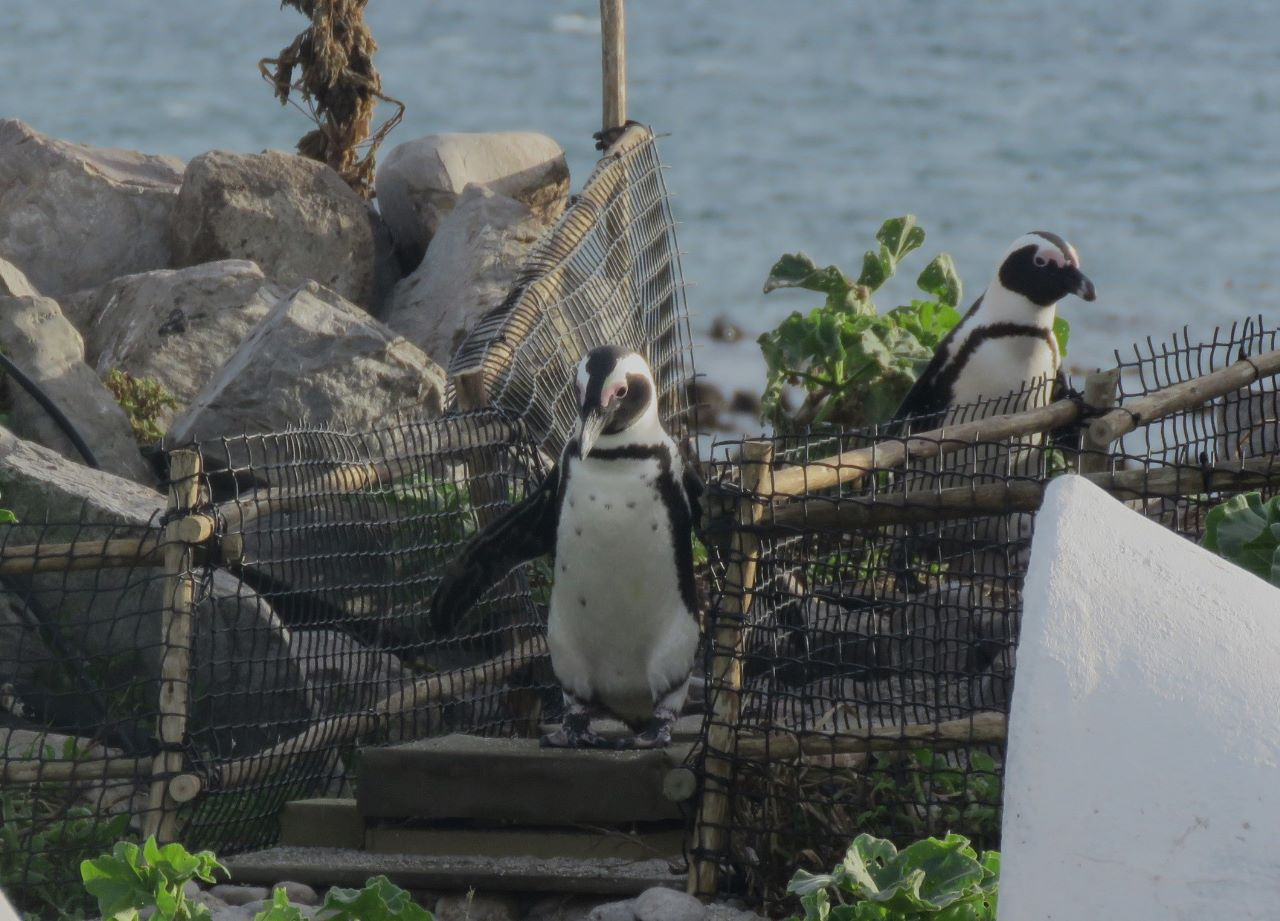
\includegraphics[keepaspectratio]{images/media/image2.jpeg}}

This manual provides a comprehensive, step-by-step guide to the
installation, configuration, and operation of the Automated Penguin
Monitoring System (APMS). Developed by BirdLife South Africa, the APMS
supports long-term monitoring of African penguin (\emph{Spheniscus
demersus}) colonies by tracking individual birds in the wild without the
stress of physical handling.

Utilizing integrated RFID detection and weighbridge technology, the
system automatically records a penguin's identity and body mass as it
passes over the weighbridge This data is transmitted to cloud storage
and processed to generate vital foraging trip metrics and body condition
indices---critical data points that directly support ecosystem-based
fisheries management.

The APMS comprises both hardware and software components. This document
is structured to guide you through building a complete system from the
ground up:

\begin{enumerate}
\def\labelenumi{\arabic{enumi}.}
\item
  \textbf{Hardware Installation} --- Setting up physical infrastructure,
  gates, and sensors.
\item
  \textbf{Software Configuration} --- Initializing the core system
  software and network connections.
\item
  \textbf{Data Processing \& Visualization} --- Deploying the data
  analysis pipelines and custom monitoring dashboard.
\item
  \textbf{Troubleshooting} --- A comprehensive diagnostic guide located
  at the end of the manual to resolve common field issues.
\end{enumerate}

\section*{How to Use This Manual}\label{how-to-use-this-manual}
\addcontentsline{toc}{section}{How to Use This Manual}

\markright{How to Use This Manual}

This manual is organised into three parts:

\begin{itemize}
\tightlist
\item
  \textbf{Hardware} --- Construction and installation of all physical
  components
\item
  \textbf{Software \& Configuration} --- Operating system setup,
  firmware, and scripts
\item
  \textbf{Deployment \& Operation} --- Field commissioning, data
  processing, and maintenance
\end{itemize}

Use the left sidebar to navigate between chapters. All chapters are
searchable using the search bar at the top of the page.

\section*{Contributing}\label{contributing}
\addcontentsline{toc}{section}{Contributing}

\markright{Contributing}

This manual is maintained as an open-source document on GitHub. To
suggest corrections or additions, use the \textbf{Edit this page} link
at the top right of any page, or open an issue on the repository.

\section*{Authors \& Acknowledgements}\label{authors-acknowledgements}
\addcontentsline{toc}{section}{Authors \& Acknowledgements}

\markright{Authors \& Acknowledgements}

Manual written by Pierre Retief for BirdLife South Africa.

\part{Overview}

\chapter{Overview}\label{overview-1}

To build the APMS, some basic tools are required. A full list can be
found at:

~~~~~~~~~~~~~~ \emph{s3://apmsbirdlife /APMS
/Documents/BirdLife\_toolkit.xlsx}

See the section AWS S3 CLOUD STORAGE for more information regarding
accessing the cloud. Please add to the tool list as/when needed. In this
manual, commands to be executed in the command line will either start
with \textbf{\emph{\$}} and be in bold and italics (for example:
\textbf{\emph{\$ sudo apt update}}) or appear in a code block as below.

\begin{Shaded}
\begin{Highlighting}[]
\FunctionTok{sudo}\NormalTok{ apt update}
\end{Highlighting}
\end{Shaded}

The APMS consists of the following key components:

\begin{itemize}
\item
  24V Solar Power Supply
\item
  4G Router
\item
  Two scales, mounted on a platform.
\item
  APMS Main Unit
\item
  BioMark RFID Reader
\end{itemize}

The 24V Solar Power Supply provides power for the APMS Main Unit,
scales, 4G Router and BioMark RFID Reader. This is site dependent.

\begin{figure}[H]

{\centering 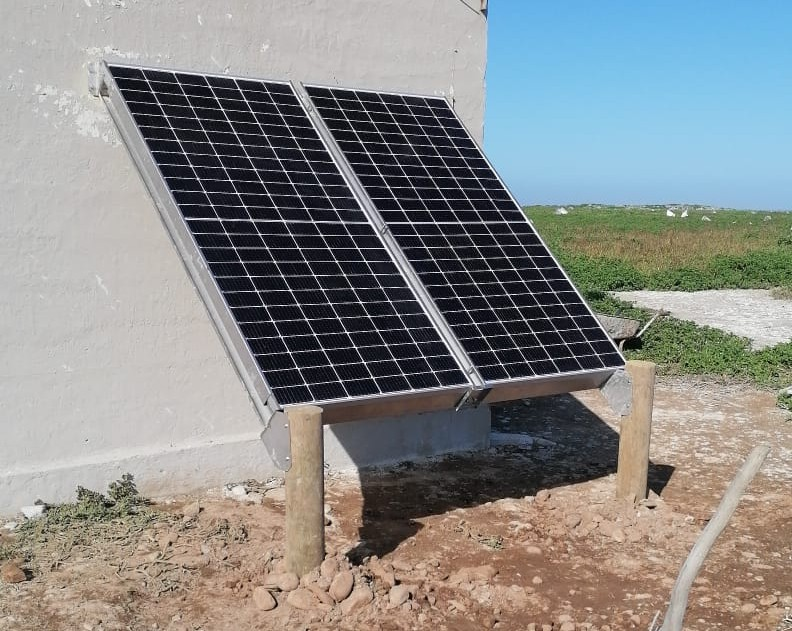
\includegraphics[width=4.16667in,height=\textheight,keepaspectratio]{images/media/01_solar_panel.jpeg}

}

\caption{Figure 1. Solar panel on Bird Island, Algoa Bay.}

\end{figure}%

The primary internet connection is provided via a 4G router. Depending
on the cellular signal strength at the site, either an indoor or outdoor
router is deployed. We prefer utilizing Teltonika
\href{https://www.teltonika-networks.com/products/routers/rut906}{RUT906}
or
\href{https://www.teltonika-networks.com/products/routers/rut956}{RUT956}
routers for two main reasons:

\begin{enumerate}
\def\labelenumi{\arabic{enumi}.}
\item
  Signal Optimization: They support external antenna cables, allowing
  the antenna to be mounted higher for improved cellular reception.
\item
  Direct Scale Integration: They feature an RS-485 port, enabling a
  direct connection to the scale indicators. This allows for remote
  control and maintenance, including remote taring and scale
  calibration.
\end{enumerate}

\begin{figure}

\begin{minipage}{0.33\linewidth}

\begin{figure}[H]

{\centering \pandocbounded{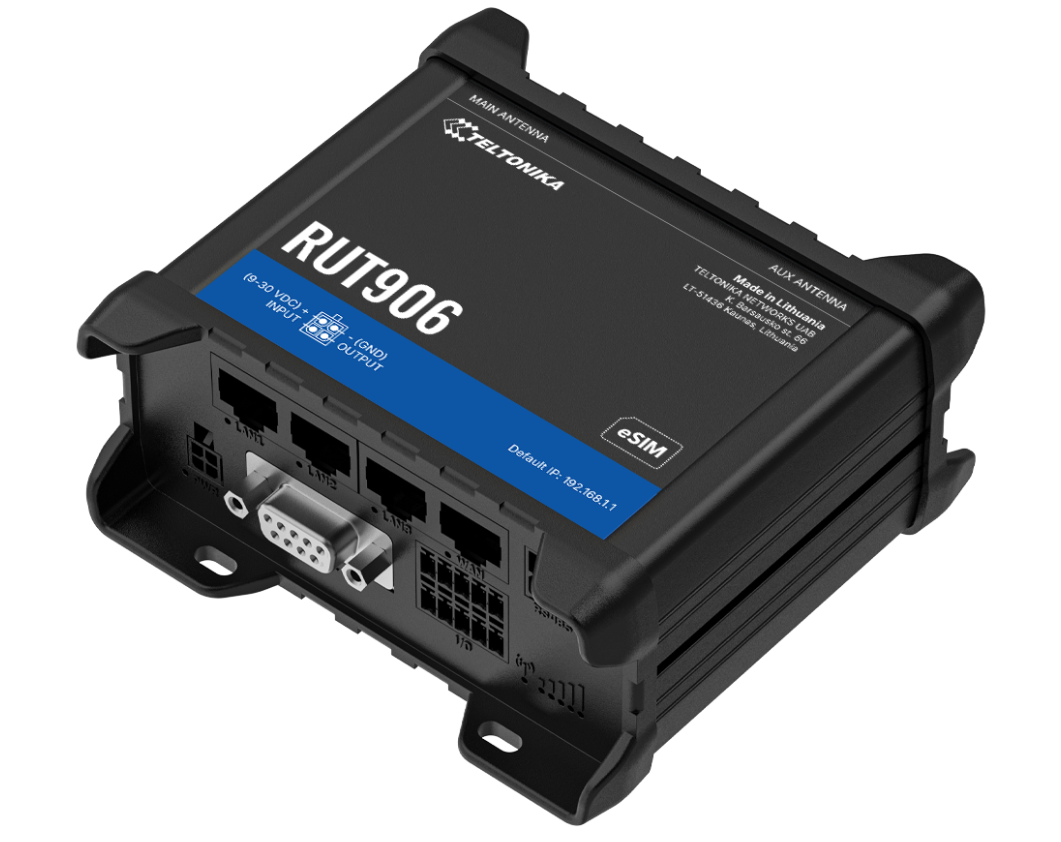
\includegraphics[keepaspectratio]{images/media/02_1_router.png}}

}

\subcaption{Figure 2.1. Teltonika RUT906}

\end{figure}%

\end{minipage}%
%
\begin{minipage}{0.33\linewidth}

\begin{figure}[H]

{\centering \pandocbounded{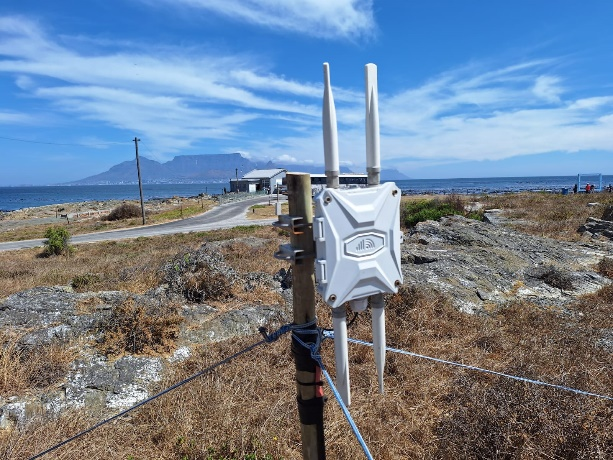
\includegraphics[keepaspectratio]{images/media/02_2_router.jpeg}}

}

\subcaption{Figure 2.2. Outdoor router}

\end{figure}%

\end{minipage}%
%
\begin{minipage}{0.33\linewidth}

\begin{figure}[H]

{\centering \pandocbounded{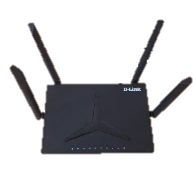
\includegraphics[keepaspectratio]{images/media/02_3_router.png}}

}

\subcaption{Figure 2.3. Indoor router}

\end{figure}%

\end{minipage}%

\end{figure}%

Two scales are used to increase accuracy and to indicate whether a
penguin is heading out to sea, or coming back from the ocean. These
scales are mounted on a platform.

\begin{figure}[H]

{\centering 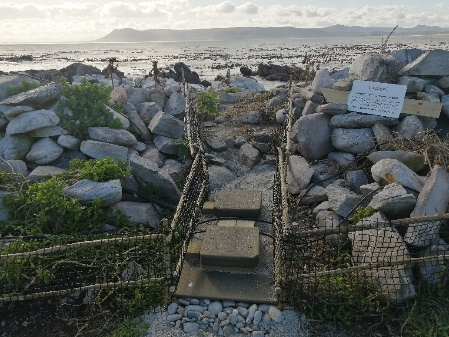
\includegraphics[width=4.16667in,height=\textheight,keepaspectratio]{images/media/03_scale_platform.jpeg}

}

\caption{Figure 3. Scale platform on Dyer Island.}

\end{figure}%

All the electronics are housed inside an IP67 rated enclosure, referred
to as the APMS Main Unit. The section ``APMS Main Unit'' describes how
to build this box.

\begin{figure}[H]

{\centering 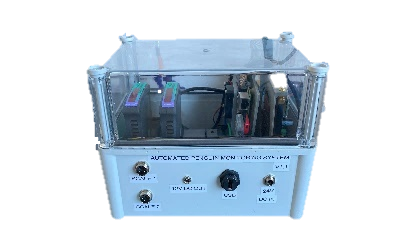
\includegraphics[width=4.16667in,height=\textheight,keepaspectratio]{images/media/04_apms_main_unit.png}

}

\caption{Figure 4. APMS main unit.}

\end{figure}%

The BioMark reader is an external device, used for picking up RFID pit
tags. The APMS connects via a USB serial interface, internal to the
reader. See the ``BioMark'' section for more information.

\begin{figure}[H]

{\centering 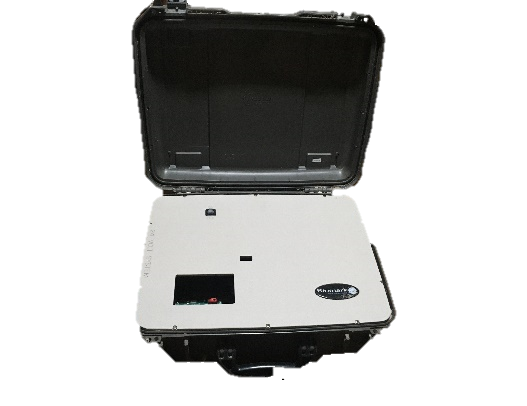
\includegraphics[width=4.16667in,height=\textheight,keepaspectratio]{images/media/05_biomark_reader.png}

}

\caption{Figure 5. BioMark reader.}

\end{figure}%

The data is downloaded daily, processed, and displayed on a Grafana
Dashboard. This is handled by the APMS Server off-site. See *** for more
information regarding the Dashboard.

\begin{figure}[H]

{\centering 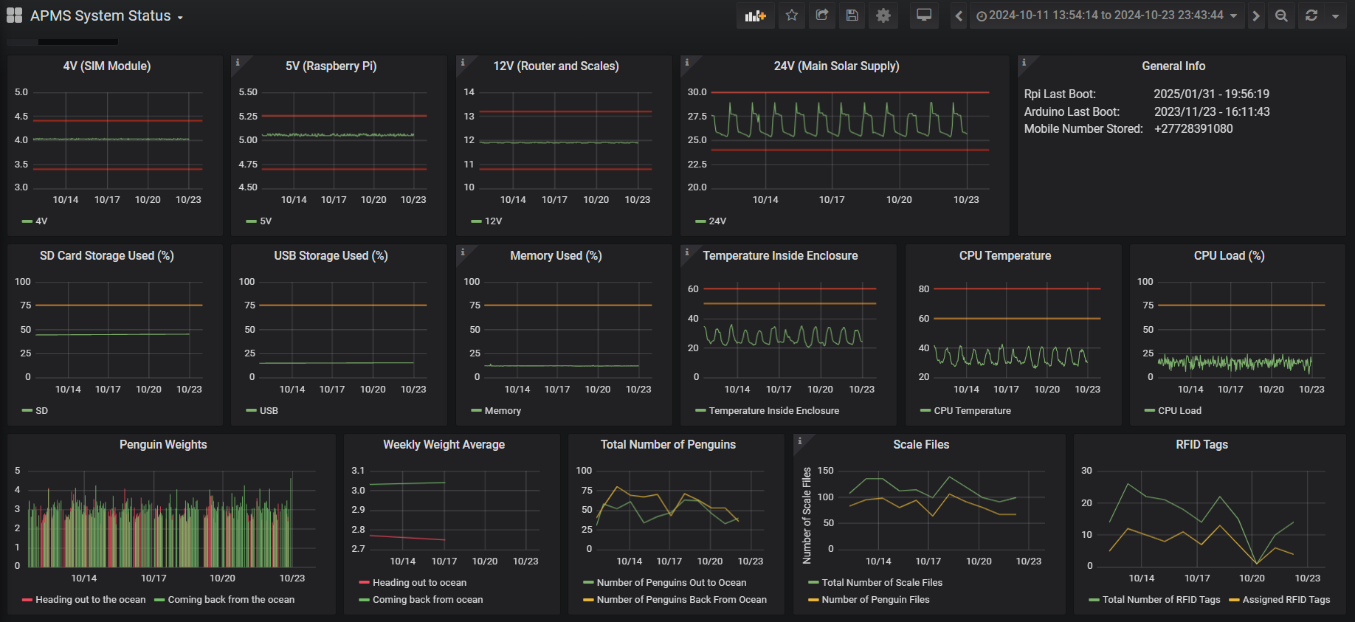
\includegraphics[width=4.16667in,height=\textheight,keepaspectratio]{images/media/06_dash.png}

}

\caption{Figure 6. APMS dashboard.}

\end{figure}%

\part{Hardware}

\chapter{Solar Power Supply}\label{solar-power-supply}

Each site is different and requires planning to ensure components are
correctly sized. A basic system and the larger system at Bird Island are
discussed below.

\section{Basic System}\label{basic-system}

A basic solar system is shown below and can be used for a site that is
running 1 BioMark RFID reader, an APMS Main Unit and a 4G Router. This
is the setup for Dassen Island, Robben Island, Stony Point and Dyer
Island. Face the solar panels North and tilt at an angle of
approximately 45 degrees. An up-to date parts list can be found at
s3://apmsbirdlife /APMS/Documents/solar\_parts\_list.xlsx

\begin{figure}[H]

{\centering 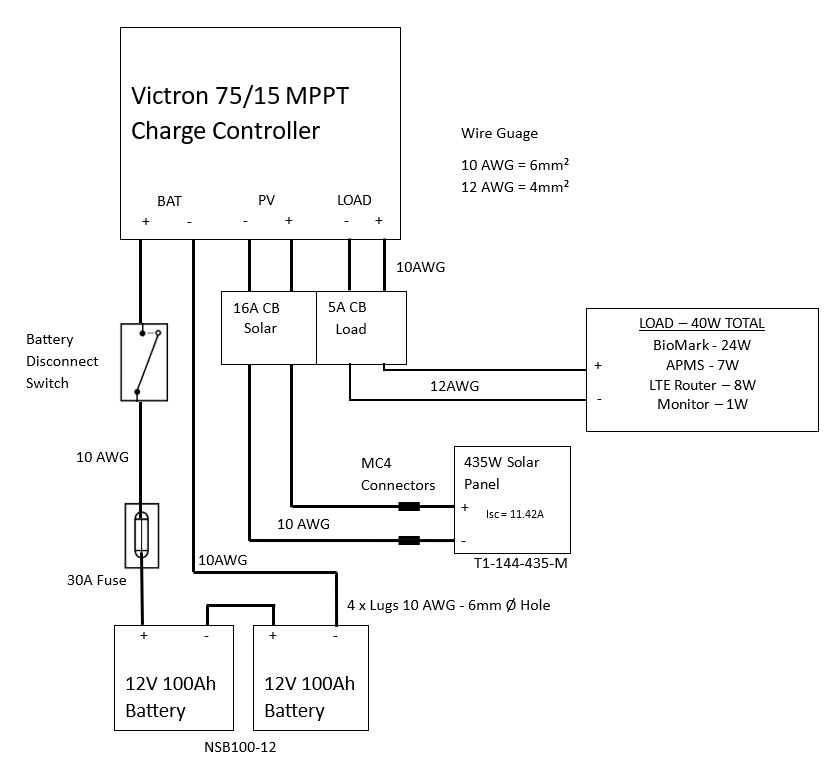
\includegraphics[width=6.9in,height=6.39583in]{images/media/07_solar.png}

}

\caption{Figure 7. A diagram of a solar power system.}

\end{figure}%

\section{Bird Island Solar System}\label{bird-island-solar-system}

The system on Bird Island is slightly larger as it is powering two
BioMark readers and has provision for a future live feed camera. See
Fig. 8 for a wiring diagram.

\begin{figure}[H]

{\centering 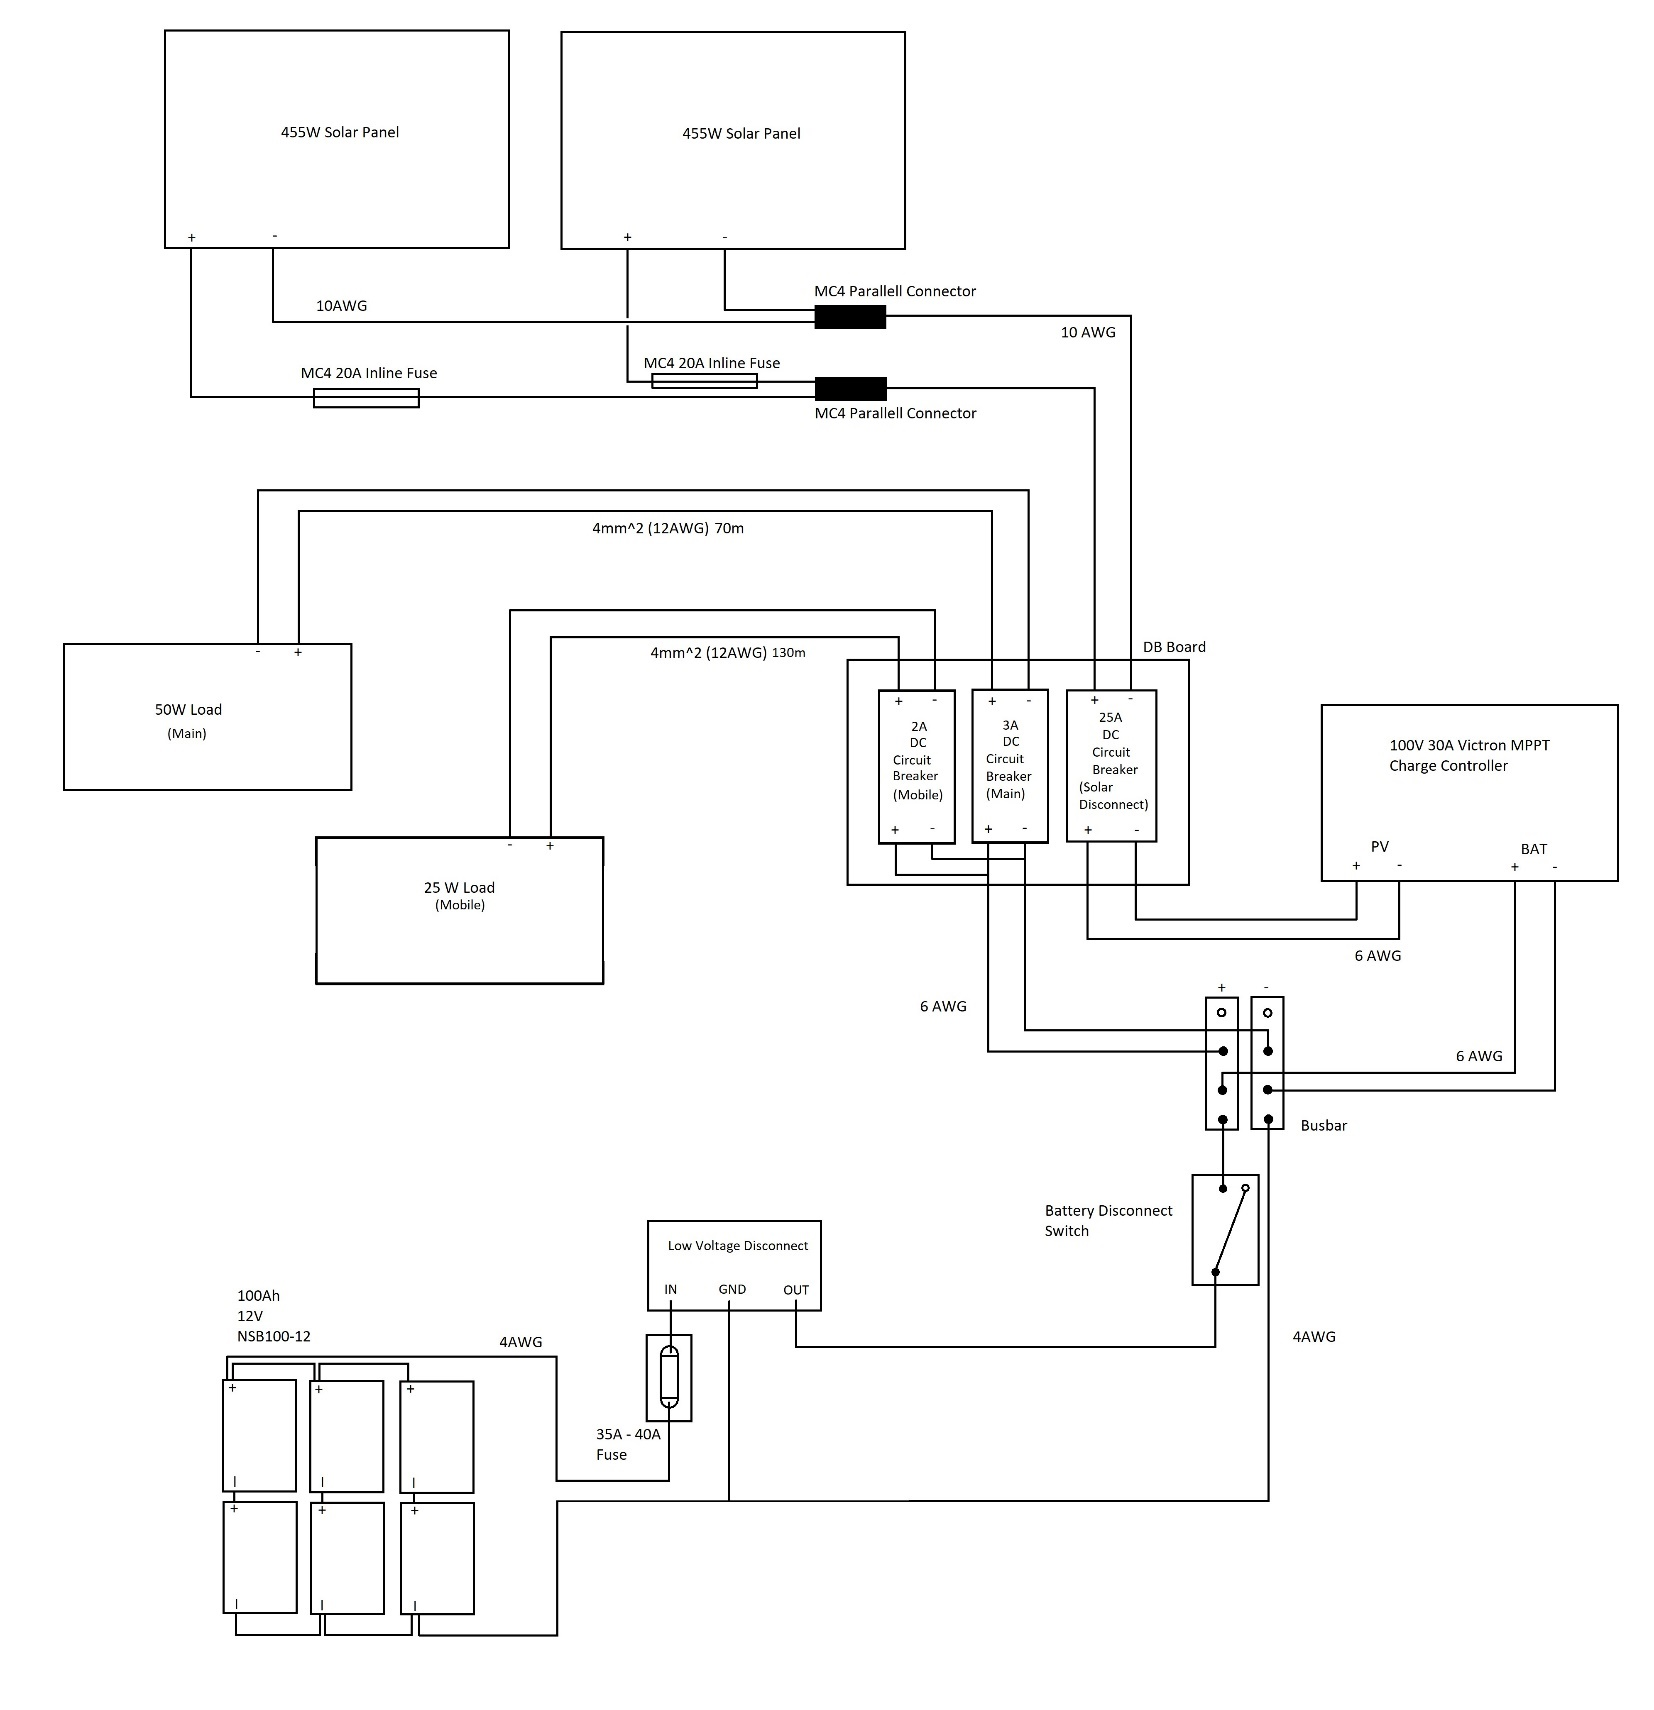
\includegraphics[width=7.51181in,height=7.77083in]{images/media/08_solar_bird.jpeg}

}

\caption{Figure 8. A diagram of the solar power supply at Bird Island,
Algoa Bay.}

\end{figure}%

\chapter{Internet and WiFi}\label{internet-and-wifi}

To monitor the site and upload data daily, a reliable internet
connection is needed. This is accomplished by using a 4G Router. Wi-Fi
has been used and has proven very reliable. If ever needed in future, a
LAN cable can be used instead.

Currently, Vodacom seems to be the strongest and most stable provider at
the different sites. The Vodacom app also makes it easy to load and keep
track of data and SMS bundles. Remember to copy down the IMEI number
from the SIM card before installing it into the router, as this number
is needed for the app.

When installing the APMS on site, take both a Vodacom and MTN SIM card,
and check which one has a better signal. Be sure to test the SIM cards
in a phone, and make sure they can access the internet.
\url{https://www.speedtest.net/} can be used to test internet
connectivity.

Depending on the site, an indoor router or outdoor router can be used,
but we recommend using one of the Teltonika routers which has more
features for maintenance and management and allows dual SIM cards.

To prepare either router for use with the APMS:

\begin{itemize}
\item
  Get a suitable SIM card, activate it, and load data.
\item
  Test the SIM in a phone to ensure it works.
\item
  Insert the SIM card into the 4G router and set up according to router
  manual.

  \begin{itemize}
  \tightlist
  \item
    Use ``apms'' as the SSID and \textless ENTER YOUR
    PASSWORD\textgreater{} as the password
  \end{itemize}
\item
  Connect to the router from a phone or PC and test the internet is
  working.
\end{itemize}

\section{Outdoor Router}\label{outdoor-router}

For more remote sites, with weaker cell reception, such as Bird and
Robben Island, an outdoor router is used. The router is purchased from
\url{https://www.outdoorrouter.com/}. Previously used model is: UK CAT6
Outdoor 4G Router (EZR33L-U4).

When ordering, ask to have a 5m DC Cable included, as we do not use 48V
POE. The cable comes with a DC connector that plugs into the circuit
board. (It needs to be bent in a slightly awkward way to fit).

\begin{figure}[H]

{\centering 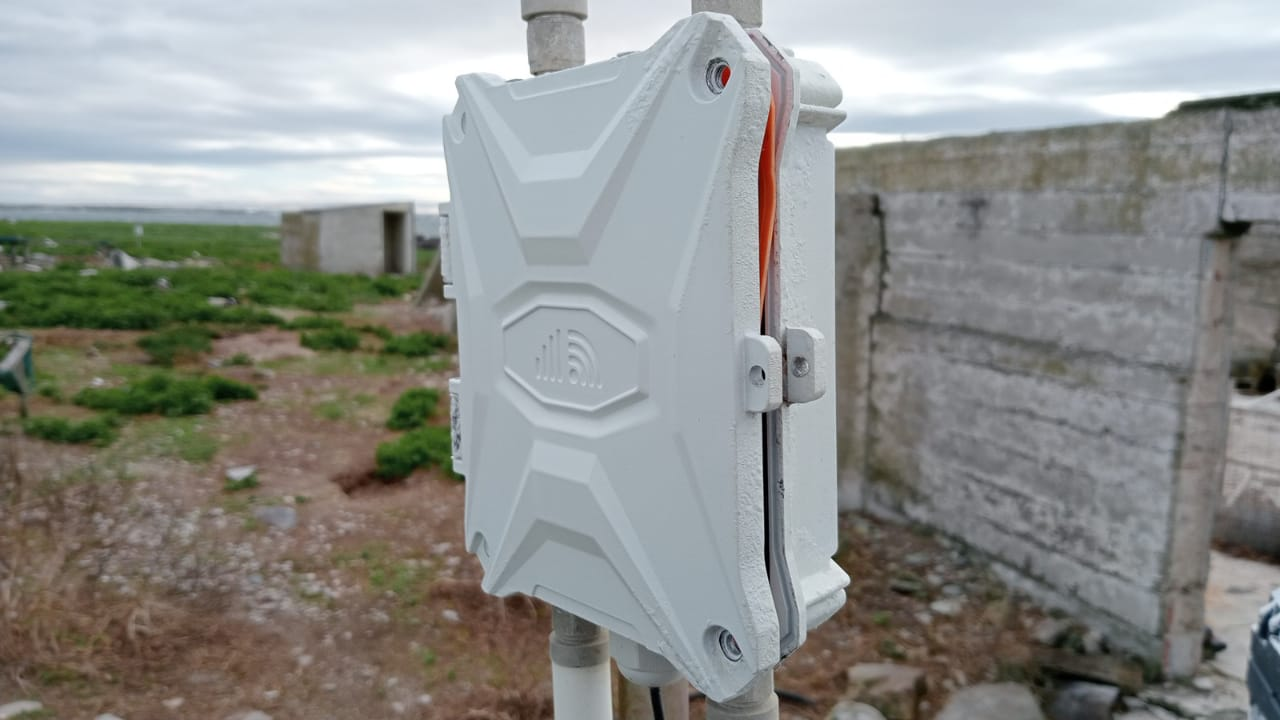
\includegraphics[width=4.16667in,height=\textheight,keepaspectratio]{images/media/09_outdoor_router.jpeg}

}

\caption{Figure 9. Outdoor router.}

\end{figure}%

The router runs directly on the 24V Solar Power supply. A circuit
breaker for the router should be installed and will also act as a power
switch, as there is no easy way to power cycle the router.

The contact person is Tammy He
(\href{mailto:tammy@outdoorrouter.com}{\nolinkurl{tammy@outdoorrouter.com}})

Mount the router on a pole or to a wall, using the hardware supplied
with the router.

Note: Check the supplied hardware and ensure that the correct bracket is
on hand before leaving for the site. Make sure to take extra nuts, bolts
and screws and test fit them to the bracket. Use stainless steel for all
fasteners. If drilling in to hard concrete, take an impact drill with,
and have extra Fischer plugs on hand.

After installation, ensure the unit is closed properly and all 4
antennas are screwed on tightly.

\section{Indoor Router}\label{indoor-router}

If the cell signal is strong enough, a cheaper indoor router can be
used. The router currently used is the DLINK DWR-M920, purchased from
Takealot. It runs on 12V DC and has external antennas for the Wi-Fi, as
well as for the cell signal. Cut off the 12V power supply and replace it
with the 12V DC plug (RS: 138-9405). This connector will plug into the
APMS Main Unit (12V DC IN) when the router is to be used.

\begin{figure}[H]

{\centering \includegraphics[width=4.16667in,height=\textheight,keepaspectratio]{images/media/10_indoor_router.jpeg}

}

\caption{Figure 10. Indoor router.}

\end{figure}%

\section{Teltonika Router}\label{teltonika-router}

\subsection{Description}\label{description}

The Teltonika RUT906 and RUT956 are industrial-grade 4G LTE routers
designed for robust connectivity in demanding remote environments.
Unlike standard commercial routers, they feature external cellular
antenna ports that allow users to connect a SMA cable, enabling a
antenna to be mounted much higher on a mast or structure to maximize
signal strength in poor coverage areas. These routers feature a built-in
RS-485 serial interface. This allows for a direct data connection to
digital scale indicators --- such as the modern General Measure GMT-X1
weight transmitter --- giving operators the ability to remotely
calibrate, tare, and configure weighing systems from anywhere in the
world without requiring a physical on-site visit.

\textbf{Additional Advantages of the RUT906/RUT956:}

\begin{itemize}
\item
  \textbf{Dual-SIM Failover:} They support two SIM cards from different
  network providers, automatically switching carriers if the primary
  network drops to guarantee continuous cloud data transmission.
\item
  \textbf{Ruggedized Design:} Housed in a durable aluminum casing, they
  are built to withstand extreme temperatures, vibrations, and harsh
  environmental conditions typical of field deployments.
\item
  \textbf{Rich I/O and Protocol Support:} Beyond RS-485, they include
  digital/analog inputs and outputs and natively support industrial
  communication protocols like Modbus, MQTT, and NTRIP.
\item
  \textbf{Low Power Consumption:} Optimized for efficiency, making them
  ideal for integration into off-grid, solar-powered battery enclosures.
\item
  \textbf{Advanced Remote Management (RMS):} Teltonika's Remote
  Management System allows for secure VPN access, batch firmware
  updates, and real-time diagnostics of the router and attached devices
  completely over-the-air.
\end{itemize}

\begin{figure}[H]

{\centering 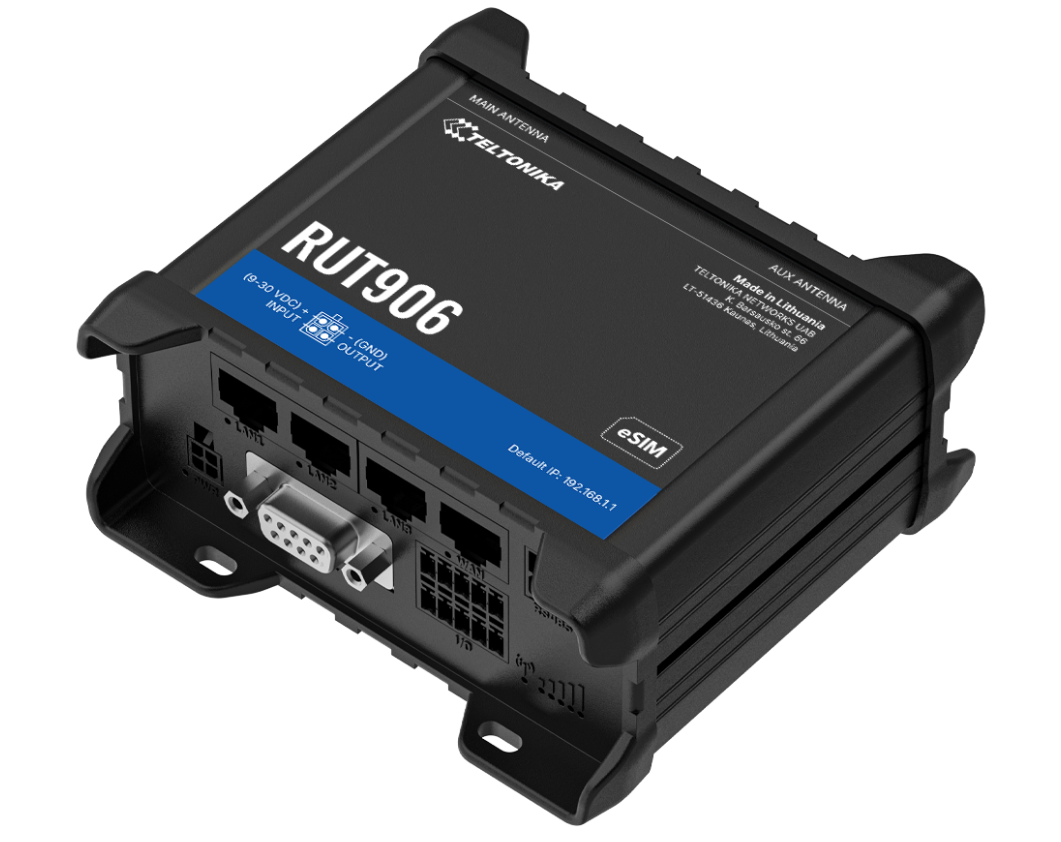
\includegraphics[width=4.16667in,height=\textheight,keepaspectratio]{images/media/10_2_router.png}

}

\caption{Figure 11. Teltonika RUT906 router.}

\end{figure}%

\subsection{Installation}\label{installation}

These routers can take a range of power supplies, from 9 -- 30 VDC, and
have reverse polarity protection. Cut off the 12V power supply (plug)
and replace it with the 12V DC plug (RS Components: 138-9405). This
connector will plug into the APMS Main Unit (12V DC IN) when the router
is to be used.

The manuals for these devices can be found here:

\begin{itemize}
\item
  \href{https://wiki.teltonika-networks.com/view/RUT906_Manual}{RUT906
  Manual}
\item
  \href{https://wiki.teltonika-networks.com/view/RUT956_Manual}{RUT956
  Manual}
\end{itemize}

\textbf{NB.} These routers are not weather protected and has to be kept
inside the APMS box or some other weather-sealed enclosure.

\chapter{Scales Platform}\label{scales-platform}

The Scales Platform consists of two scales, mounted on a wooden base,
with a RFID Antenna running through the middle. There are two ``cable
guides'' to guide the scale cables and keep it in place.

\section{Overview}\label{overview-2}

The scales are manufactured by R\&D WEIGHING (PTY) LTD
\href{mailto:accounts@rdweighing.co.za}{(accounts@rdweighing.co.za)}.

Depending on the distance between the scales and the Main Unit, extra
scale cable might be needed and you will have to specify this in your
order. The company can also solder the extended cable if needed. 5kg and
1kg calibrated weights are also purchased from R\&D Weighing and are
used for scale calibration. Please find a suitable enclosure for the
weights and keep them indoors to prevent corrosion or damage. A parts
list can be seen in TABLE 1 - SCALES PLATFORM PARTS LIST and the drawing
can be seen in FIGURE 12 - DRAWING OF SCALES PLATFORM.

\begin{longtable}[]{@{}
  >{\raggedright\arraybackslash}p{(\linewidth - 6\tabcolsep) * \real{0.2500}}
  >{\raggedright\arraybackslash}p{(\linewidth - 6\tabcolsep) * \real{0.2500}}
  >{\raggedright\arraybackslash}p{(\linewidth - 6\tabcolsep) * \real{0.2500}}
  >{\raggedright\arraybackslash}p{(\linewidth - 6\tabcolsep) * \real{0.2500}}@{}}
\caption{Scales platform parts
list}\label{tbl-scales-parts}\tabularnewline
\toprule\noalign{}
\begin{minipage}[b]{\linewidth}\raggedright
Name
\end{minipage} & \begin{minipage}[b]{\linewidth}\raggedright
Quantity
\end{minipage} & \begin{minipage}[b]{\linewidth}\raggedright
Description
\end{minipage} & \begin{minipage}[b]{\linewidth}\raggedright
Where to buy / Part Number
\end{minipage} \\
\midrule\noalign{}
\endfirsthead
\toprule\noalign{}
\begin{minipage}[b]{\linewidth}\raggedright
Name
\end{minipage} & \begin{minipage}[b]{\linewidth}\raggedright
Quantity
\end{minipage} & \begin{minipage}[b]{\linewidth}\raggedright
Description
\end{minipage} & \begin{minipage}[b]{\linewidth}\raggedright
Where to buy / Part Number
\end{minipage} \\
\midrule\noalign{}
\endhead
\bottomrule\noalign{}
\endlastfoot
Scale & 2 & Stainless Steel scale with B6N load cell &
\href{https://www.rdweighing.co.za/}{R\&D Weighing} \\
Indicator & 2 & (General measure) GMT-X1 Or the Laumas TLB485 &
\href{https://www.rdweighing.co.za/}{R\&D Weighing} \\
1 kg weight & 1 & Used for calibration &
\href{https://www.rdweighing.co.za/}{R\&D Weighing} \\
5 kg weight & 1 & Used for calibration &
\href{https://www.rdweighing.co.za/}{R\&D Weighing} \\
Scale Cable & as needed & Extra scale cable (optional) &
\href{https://www.rdweighing.co.za/}{R\&D Weighing} \\
Base board & 1 & Base of platform. Marine Ply 1200x500x15mm &
\href{https://timbuildwoodstock.co.za/plywoods/}{TimBuild Woodstock} \\
Cable guide & 2 & To guide scale cable, wood & Hardware store --
Builders Warehouse \\
RFID block & 1 & RFID mounting block to hold antenna, wood & Hardware
store -- Builders Warehouse \\
6 pin plug & 2 & Plug to connect scale to Main Unit & RS: 111-5758 \\
Canvas & ±4m & To cover everything. Olive/Dark Green &
\href{https://www.ludalinterior.co.za/}{Ludal Interior} \\
\end{longtable}

\section{Scales}\label{scales}

The scales consist of a stainless-steel frame with a type B6N loadcell
mounted underneath. A pan rests on top of the frame to provide a flat
surface for the penguins to walk over. Note that the scales at Stony
Point and Bird Island have older frames that are 90 degrees with respect
to the new scales. If the scales need to be replaced in future, new
holes can be drilled in the platform. Usually, however, only the load
cell needs to be replaced and thus the existing frame can be re-used.

\begin{figure}[H]

{\centering 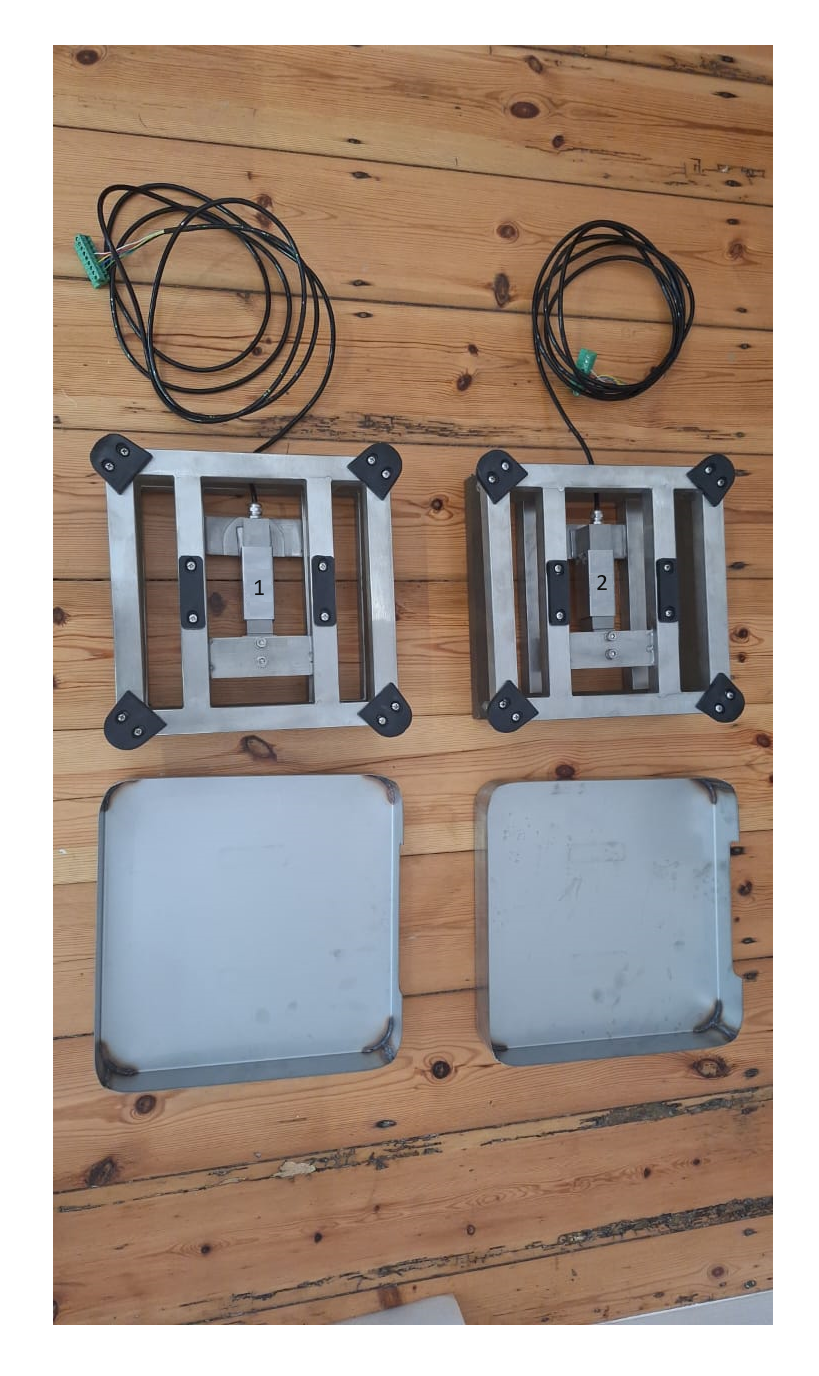
\includegraphics[width=4.16667in,height=\textheight,keepaspectratio]{images/media/13_scale_frames.png}

}

\caption{\textbf{Figure 13.} Scale frames with monuted loadcell and
scale pans.}

\end{figure}%

The initial systems (Stony Point and Bird Island) used 50kg load cells.
For the two newer systems (Dyer Island and Robben Island), a more
sensitive 30kg load cell is used. However, it's recommended to use a
load cell with a higher load such as the 100kg load cell so that if a
person accidentally steps on it in the field it won't break (unless that
person is 150\% of the load cell's weight rating, i.e., 150kg). The
difference in sensitivity between 30, 50 and 100kg load cells are not
significant.

\begin{figure}[H]

{\centering 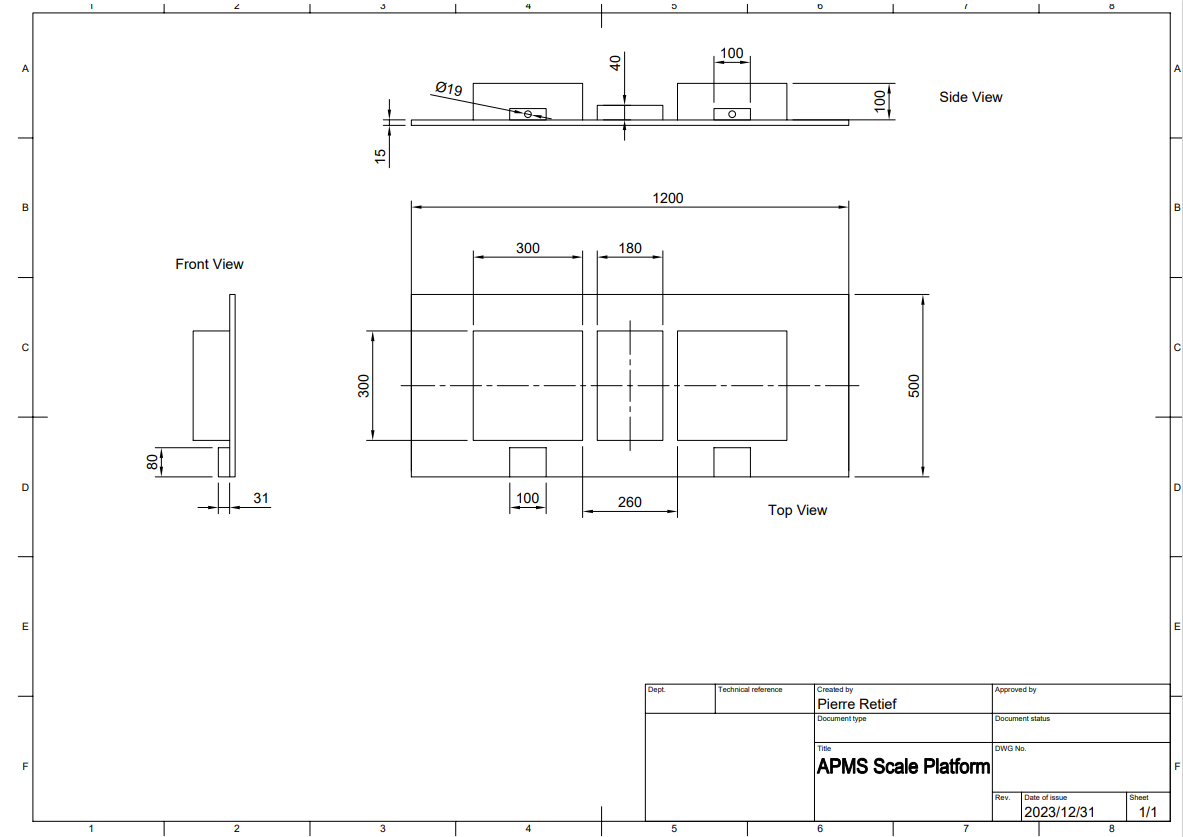
\includegraphics[width=7.29167in,height=\textheight,keepaspectratio]{images/media/14_scales_drawing.png}

}

\caption{\textbf{Figure 14.} Drawing of scales platform.}

\end{figure}%

\begin{figure}[H]

{\centering 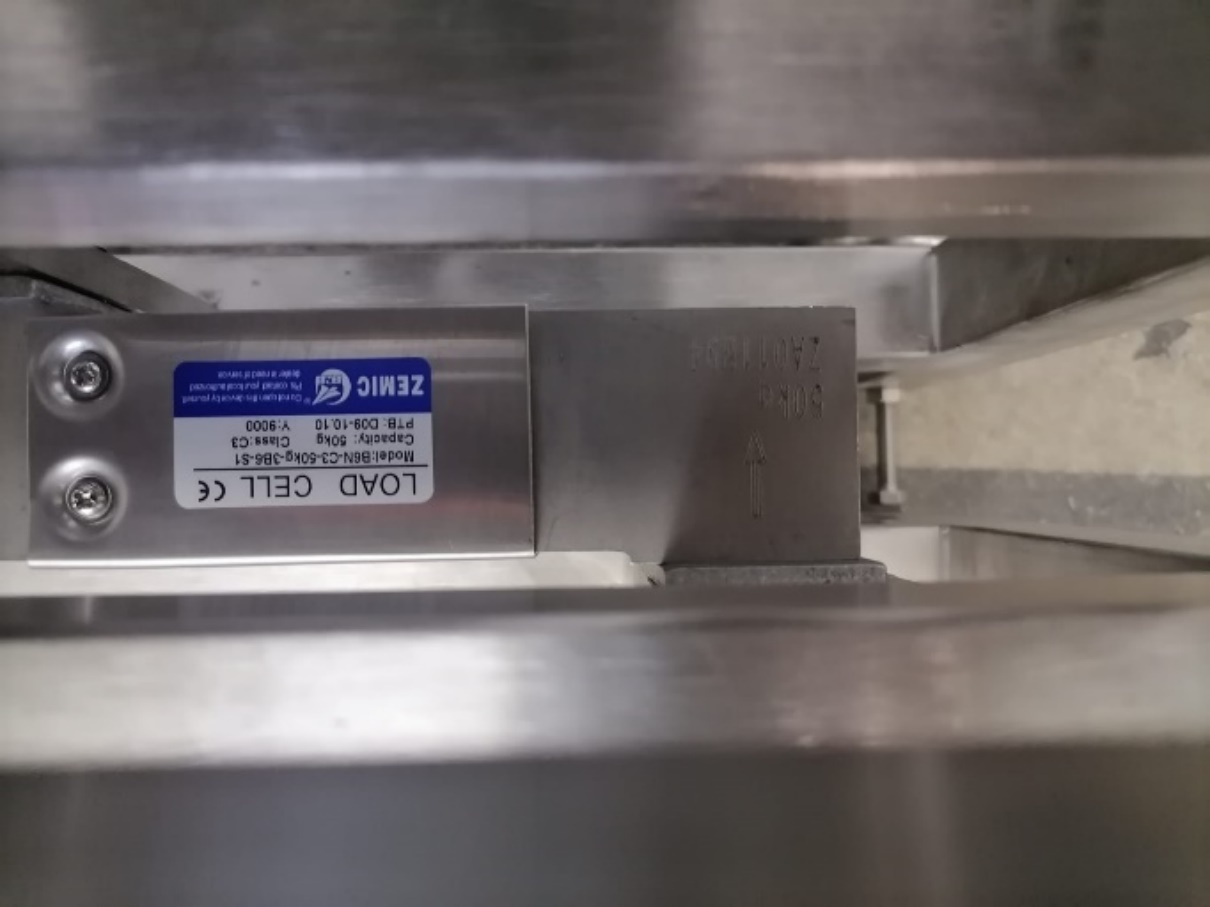
\includegraphics[width=4.16667in,height=\textheight,keepaspectratio]{images/media/15_loadcell.jpeg}

}

\caption{\textbf{Figure 15.} Load cell mounted on a scale paltform.}

\end{figure}%

Note: The maximum safe loading weight of the load cell is 150\%. Thus,
for a 50kg load cell, the max load is 75kg, for the 30kg load cell, the
max load is 45kg, and for a 100kg load cell, the max load is 150kg.

\section{Building the Platform}\label{building-the-platform}

Start by gathering all the required parts for the platform.

\begin{figure}[H]

{\centering 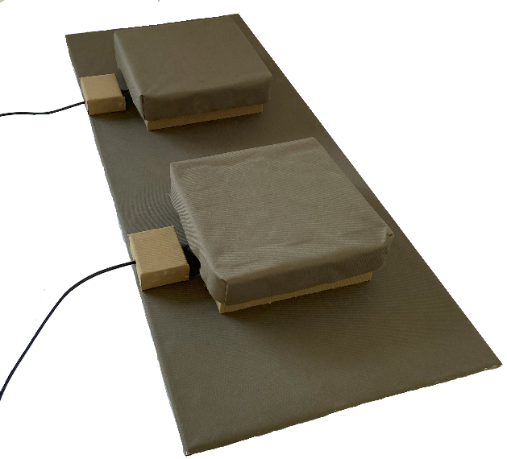
\includegraphics[width=4.16667in,height=\textheight,keepaspectratio]{images/media/16_platform.png}

}

\caption{\textbf{Figure 16.} Scale platform covered in canvas.}

\end{figure}%

Take note of the following while building the platform:

\begin{itemize}
\item
  Label the scales and indicators immediately upon removing them from
  their packaging, as the scales and indicators are tied to each other.
\item
  Cover the wooden base and scales with canvas. The canvas can be glued
  to the wood and scales using Contact adhesive. Silicon has also been
  used. The cable guides and RFID block can be screwed down from
  underneath.
\item
  The scales are mounted using the threaded holes where the feet used to
  screw in.
\item
  Mount the scales to the base using 4 \hl{***}mm bolts per scale.
\item
  Scale 1 is positioned on the colony side, and Scale 2 is positioned on
  the ocean side. To remember this layout, consider a chick's natural
  life cycle: a penguin is hatched on land (colony side) and will walk
  over Scale 1 first when heading out to sea for its very first foraging
  trip.
\item
  The distance between the \ul{pans} of the scales is set to 26 cm.
\item
  It is important to ensure the frame of the scale is flush with the
  base.
\item
  Cover the cable guides with canvas and secure to the base. Feed the
  scale cables through the cable guide. See FIGURE 15 - SCALES PLATFORM
  WITHOUT RFID BLOCK
\item
  Cover the RFID Mounting Block with canvas and secure it between the
  scales. Drill holes to allow zip ties to be used to clamp the RFID
  antenna to the block.
\item
  Solder a 6-pin socket (RS Components part number: 111-5764) to the end
  of each scale cable. This will plug into the 6-pin connector on the
  APMS Main Unit.
\item
  After the Scale Indicators have been installed and configured, test
  and calibrate the platform on a solid, level floor. This will confirm
  the scales are 100\% functional before taking it to the field. See
  INSTALLING THE SCALE INDICATORS and ROUTINE CALIBRATION OF SCALES for
  more information.
\end{itemize}

\begin{figure}[H]

{\centering 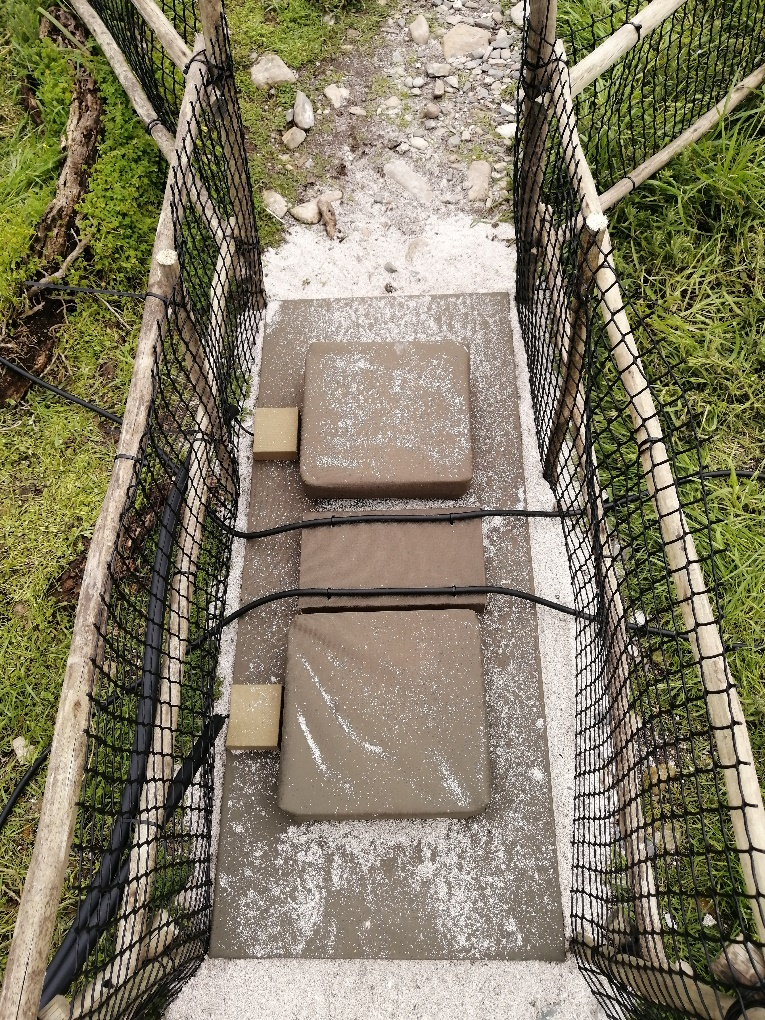
\includegraphics[width=6.25in,height=\textheight,keepaspectratio]{images/media/17_complete_platform.jpeg}

}

\caption{\textbf{Figure 17.} A completed scales platform with an RFID
antenna running through the middle of the two scales.}

\end{figure}%

\chapter{APMS Monitor}\label{apms-monitor}

A separate circuit, called the APMS Arduino Monitor, or just ``Monitor''
for short, is used to constantly check different system parameters, and
gives the administrator the ability to diagnose system faults remotely.

All the components needed to build the Monitor are listed in Table 2 -
APMS Monitor Parts List. A website or RS part number is given, accurate
at time of writing this manual.

The circuit diagram can be seen in FIGURE 17 - APMS ARDUINO MONITOR
CIRCUIT DIAGRAM

\begin{longtable}[]{@{}
  >{\raggedright\arraybackslash}p{(\linewidth - 8\tabcolsep) * \real{0.2200}}
  >{\raggedright\arraybackslash}p{(\linewidth - 8\tabcolsep) * \real{0.1800}}
  >{\raggedright\arraybackslash}p{(\linewidth - 8\tabcolsep) * \real{0.1300}}
  >{\raggedright\arraybackslash}p{(\linewidth - 8\tabcolsep) * \real{0.1100}}
  >{\raggedright\arraybackslash}p{(\linewidth - 8\tabcolsep) * \real{0.3400}}@{}}
\caption{\textbf{Table 2} - APMS Monitor Parts List}\tabularnewline
\toprule\noalign{}
\begin{minipage}[b]{\linewidth}\raggedright
\textbf{Name}
\end{minipage} & \begin{minipage}[b]{\linewidth}\raggedright
\textbf{Designation}
\end{minipage} & \begin{minipage}[b]{\linewidth}\raggedright
\textbf{Quantity per board}
\end{minipage} & \begin{minipage}[b]{\linewidth}\raggedright
\textbf{RS Part Number}
\end{minipage} & \begin{minipage}[b]{\linewidth}\raggedright
\textbf{Notes}
\end{minipage} \\
\midrule\noalign{}
\endfirsthead
\toprule\noalign{}
\begin{minipage}[b]{\linewidth}\raggedright
\textbf{Name}
\end{minipage} & \begin{minipage}[b]{\linewidth}\raggedright
\textbf{Designation}
\end{minipage} & \begin{minipage}[b]{\linewidth}\raggedright
\textbf{Quantity per board}
\end{minipage} & \begin{minipage}[b]{\linewidth}\raggedright
\textbf{RS Part Number}
\end{minipage} & \begin{minipage}[b]{\linewidth}\raggedright
\textbf{Notes}
\end{minipage} \\
\midrule\noalign{}
\endhead
\bottomrule\noalign{}
\endlastfoot
Strip board 100 x 160 mm & & 1 & 206-5879 & RS Components \\
Fuse holder & FH1 & 1 & 765-2973 & Min Order Quantity: 5 \\
3A fuse & F1 & 1 & 668-5963 & Min Order Quantity: 10 \\
Monitor Mounting Plate & & 1 & & 3D Printed. Design files on AWS S3 \\
PCB Screw Terminal & J1, J2 & 2 & 193-0564 & Min Order Quantity: 5 \\
SIM800L-V2 5V & U2 & 1 & & https://www.robotics.org.za/SIM800L-V2 \\
1uF Capacitor & C1 & 1 & 538-1578 & Min Order Quantity: 5 \\
33pF Capacitor & C2 & 1 & 194-0457 & Min Order Quantity: 10 \\
10pF Capacitor & C3 & 1 & 194-0443 & Min Order Quantity: 10 \\
1000uF Capacitor & C4 & 1 & 711-1150 & Min Order Quantity: 10 \\
5.1V Zener & D1 & 1 & 544-3597 & Min Order Quantity: 20 \\
10uF 50V Capacitor & C5 & 1 & 811-8373 & Min Order Quantity: 5 \\
K7805 Voltage Regulator 500mA & U3 & 1 & 757-7239 144-6290 & RS
Components \\
22uF Capacitor & C6 & 1 & 190-2953 & Min Order Quantity: 10 \\
Arduino Nano Every & U4 & 1 & 192-7586 & RS Components \\
Push Button & SW1 & 1 & 135-9445 & Min Order Quantity: 20 \\
10k Trimpot & RV1 & 1 & 769-2202 & RS Components \\
Temperature Sensor & U5 & 1 & 811-5595 & Min Order Quantity: 10 \\
NPN Transistor KSP2222ABU & Q1, Q2 & 2 & 739-0385 & Min Order Quantity:
10 \\
Resistor 22k & R9 & 1 & 135-954 & Min Order Quantity: 10 \\
Resistor 10k & R4, R10 & 2 & & https://www.prototypediy.co.za/ \\
Resistor 4k7 & R8 & 1 & & https://www.prototypediy.co.za/ \\
Resistor 27k & R3, R6 & 2 & & https://www.prototypediy.co.za/ \\
Resistor 5k6 & R5, R7 & 2 & & https://www.prototypediy.co.za/ \\
Resistor 6k8 & R2 & 1 & & https://www.prototypediy.co.za/ \\
Resistor 1k2 & R1, R11 & 2 & & https://www.prototypediy.co.za/ \\
LM2596 DC-DC Converter & U1 & 1 & & www.netram.co.za \\
Logic Level Converter & U6 & 1 & & https://www.netram.co.za \\
40 Pin Header Socket for Pi & J3 & 1 & 674-1252 & RS Components \\
36 Pin Male Headers & & 5 & 547-3166 & RS Components \\
30 Pin Female Header & & 2 & 767-9842 & RS Components \\
Schottky Diode & D2 & 1 & 168-7175 & comes in pack of 10 \\
40 Pin Ribbon Cable & & 1 & & www.pishop.co.za \\
Buzzer & BZ1 & 1 & 771-6957 & comes in pack of 5 \\
M2.5 x 8mm machine screws & & 4 & 914-1567 & RS Components \\
\end{longtable}

\begin{figure}[H]

{\centering 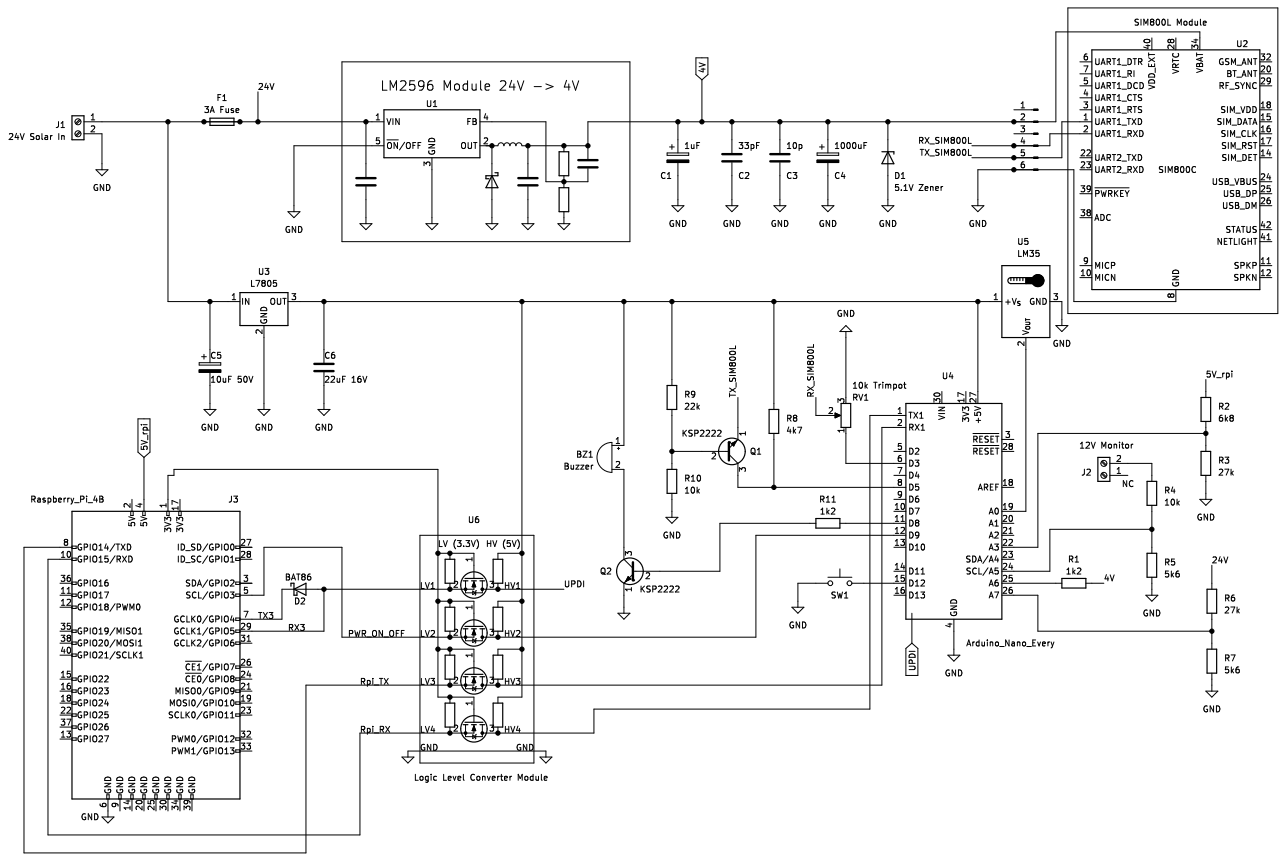
\includegraphics[width=7.29167in,height=\textheight,keepaspectratio]{images/media/18_circuitdiagram_v1.png}

}

\caption{\textbf{Figure 18.} Circuit diagram of the APMS Monitor
(version 1). In version 2 the SIM800L is replaced by a SIM800L-V2 module
which no longer needs the 4V conversion.}

\end{figure}%

\subsection{Overview}\label{overview-3}

The Monitor uses a separate SIM card and can thus be used to fault find
the system even when the main internet is down. The Arduino can be
programmed through the Raspberry Pi once configured. Currently, the main
features are:

\begin{itemize}
\item
  Monitors the 4V internal power supply, used to power the SIM card
  module (only version 1 of the monitor board, version 2 uses a 5V SIM
  module and hence no longer needed to convert to and monitor 4V).
\item
  Monitors the 5V power supply, used to power the Raspberry Pi.
\item
  Monitors the 12V power supply, used for the scales and router (i.e.,
  the indoor or teltonika router).
\item
  Monitors the 24V solar power supply.
\item
  Monitors the ambient temperature inside the APMS Main Unit.
\item
  Alerts the administrator when the Monitor or Raspberry Pi boots up via
  SMS.
\item
  Shut down and power up the Raspberry Pi via SMS.
\item
  Send an APMS status report on request via SMS.
\item
  Exchanges status reports with the Raspberry Pi every hour.
\end{itemize}

As the Monitor circuit is still a prototype, with relatively few
components, the board is built on a piece of stripboard directly from
the circuit diagram. Five boards have been built thus far, one for Stony
Point, Bird Island, Dyer Island, Robben Island and Dassen Island. A PCB
is being designed for future APMS installations.

As most components are quite standard, it should not be hard to source
parts or find suitable replacements.

The circuit board is mounted on a custom designed, 3D printed Monitor
Mounting Plate. The mount has been designed to fit the existing DIN
rail, for easy insertion/extraction. The mounting plate is printed with
ABS plastic to prevent warping in the summer heat. The design file for
3D printing can be downloaded here:
\href{files/Monitor_V_0_5.3mf}{Download}

\subsection{Programming via the Arduino
Software}\label{programming-via-the-arduino-software}

The heart of the circuit is the Arduino Nano Every microcontroller. This
is the successor to the popular Arduino Nano and provides slightly
better capabilities for a lower price. The Arduino can be programmed in
numerous ways. Two ways are discussed in this manual. The first will be
using an unaltered Arduino and the standard Arduino Software, while the
second method involves using the Raspberry Pi, together with some
hardware modifications to the Arduino.

\begin{itemize}
\item
  Before building the circuit, it is a good idea to test the Arduino. As
  the Arduino is straight out of the box, the standard Arduino software
  will be used for the initial setup.

  \begin{itemize}
  \item
    Install the Arduino IDE Software
    (https://www.arduino.cc/en/software)
  \item
    Install the Arduino megaAVR Core:

    \begin{itemize}
    \item
      From the Tools menu, select ``Boards''
    \item
      Select ``Boards Manager''
    \item
      Search for and install ``megaAVR''
    \end{itemize}
  \item
    Download the test sketch from here:
    \href{files/monitor_test_sketch.ino}{Download}
  \item
    Use a Micro USB cable to connect to the Arduino and select the
    appropriate com port
  \item
    Click ``Upload''
  \item
    If the upload was successful, the LED will light up and the buzzer
    will sound when the button is pressed.
  \item
    If the upload fails try a different com port, or charge the
    registers emulation:

    \begin{itemize}
    \tightlist
    \item
      Tools \textgreater{} Register Emulation \textgreater{} None
      (ATMEGA4809)
    \end{itemize}
  \end{itemize}
\end{itemize}

\textbf{NOTE: If the Arduino has already been modified for UPDI,
programming via the USB port will not be possible. First remove the
soldered link and disconnect the UPDI wire. See UPDI PROGRAMMING for
more details}

\subsection{Preparing the Stripboard}\label{preparing-the-stripboard}

The 100x160 mm stripboard needs to be reduced to fit inside the Main
Unit.

\begin{itemize}
\item
  Mark the four corners for drilling with a permanent marker. The
  locations of the holes are important as they correspond to the holes
  in the mounting plate. See FIGURE 19 -- PREPARING THE STRIPBOARD
\item
  The board does not have to be broken at the line, as seen in the
  picture, and a larger PCB can be obtained by breaking off a smaller
  piece. Just ensure the spacing between the holes are correct, as in
  the picture.
\end{itemize}

\begin{figure}[H]

{\centering 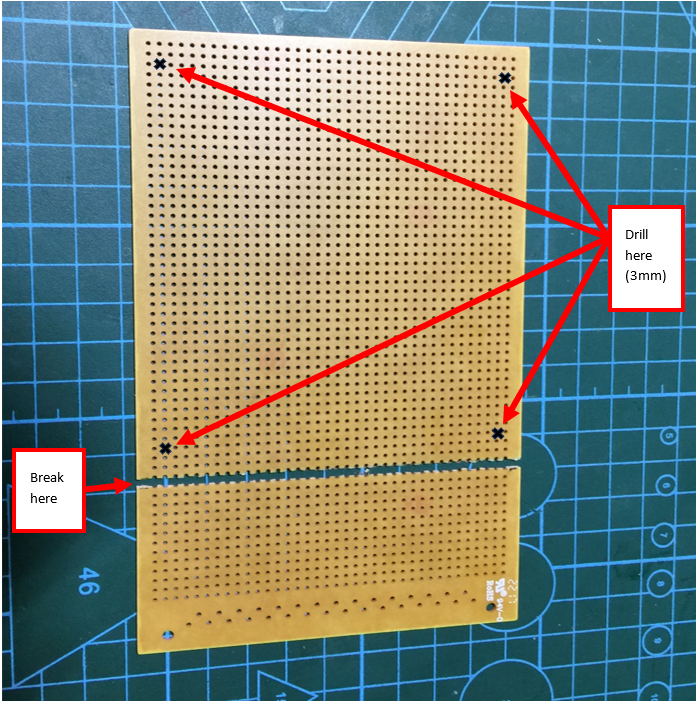
\includegraphics[width=4.16667in,height=\textheight,keepaspectratio]{images/media/19_stripboard.png}

}

\caption{\textbf{Figure 19.} Preparing the stripboard.}

\end{figure}%

\begin{itemize}
\item
  Use the 3mm drill bit to drill the four corner holes in the circuit
  board.

  \begin{itemize}
  \tightlist
  \item
    Do a test fit as shown in fig.~20. Use the four 2.5mm machine screws
    to secure the blank circuit board to the mounting plate.
    \textbf{Note, do not exert too much force as the screws are going
    into plastic.}
  \end{itemize}
\end{itemize}

\begin{figure}[H]

{\centering 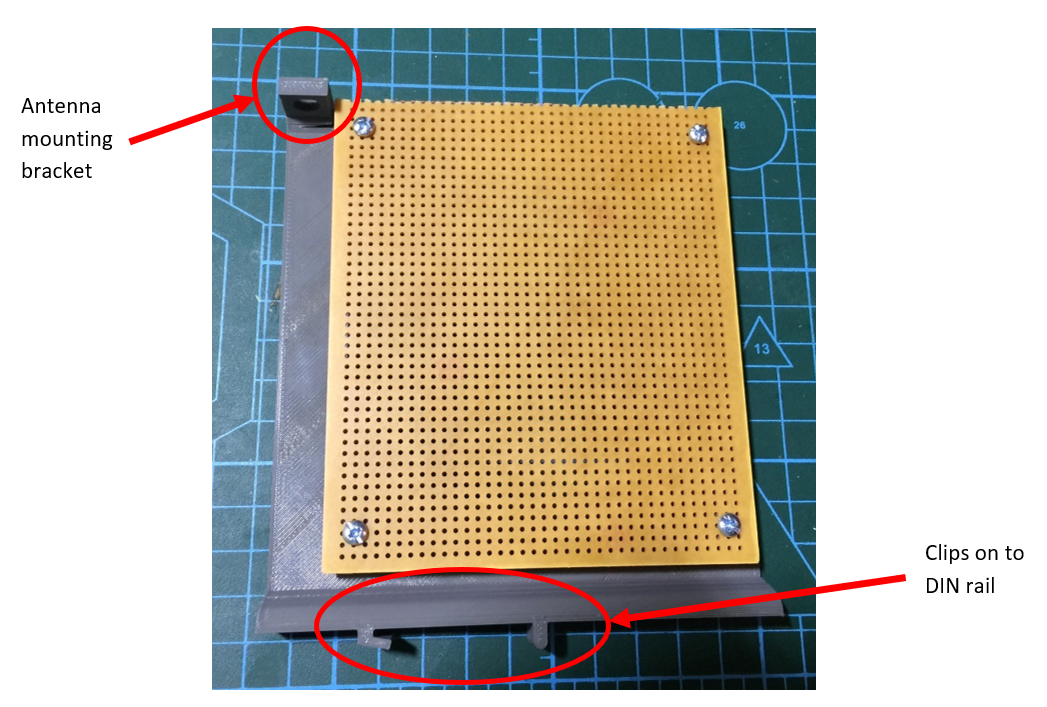
\includegraphics[width=4.16667in,height=\textheight,keepaspectratio]{images/media/20_test_stripboard.png}

}

\caption{\textbf{Figure 20.} Test fit the blank board on the mounting
bracket.}

\end{figure}%

\begin{itemize}
\item
  The SIM800L antenna can be installed on the mounting bracket provided.
\item
  If the signal at the site is particularly weak, an antenna with higher
  gain can be used. For example:

  \begin{itemize}
  \tightlist
  \item
    An omnidirectional antenna (RS Part Number: 202-4179).
  \item
    A blade antenna with a SMA extension cable.
  \end{itemize}
\item
  Remove the blank circuit board from the mounting plate and start
  building the circuit according to the circuit diagram.
\end{itemize}

\subsection{4V and 5V Power Supplies}\label{v-and-5v-power-supplies}

\begin{itemize}
\item
  Start with the main 24V DC connector and fuse holder.
\item
  \textbf{Skip this step if you are building version 2 of the monitor
  board. In version 2 of the APMS monitor, we no longer need the LM2596
  converter as a different SIM module is used which runs on 5V.} If you
  are building version 1 of the monitor board, then also add the LM2596
  DC-DC converter and then insert a 3A fuse into the fuse holder. Next
  provide 24V to the main DC connector and adjust the output voltage of
  the LM2596 DC-DC converter to 4.0 V.
\item
  Install the K7805 voltage regulator, capacitors C5 and C6 and check
  for 5V on the output.
\item
  Break one of the 30 pin female header strips in half, to obtain two 15
  pin strips. Use these two strips as a socket for the Arduino Nano (see
  fig.~21).
\item
  Test for 5V between the GND and VCC pins on the Arduino header. Do not
  install the Arduino yet.
\end{itemize}

\begin{figure}[H]

{\centering 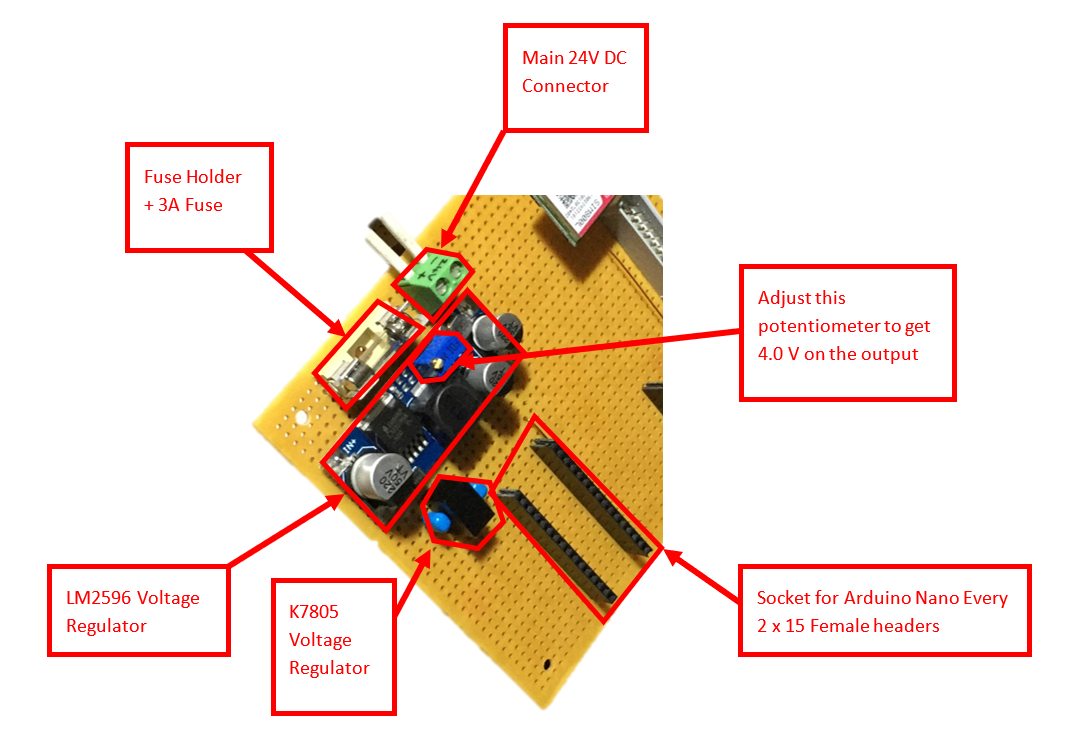
\includegraphics[width=6.25in,height=\textheight,keepaspectratio]{images/media/21_partial_monitor.png}

}

\caption{\textbf{Figure 21.} A partially built monitor (version 1) for
Stony Point.}

\end{figure}%

\subsection{SIM800L Power Supply}\label{sim800l-power-supply}

\begin{itemize}
\item
  The version 1 Monitor uses a SIM800L module (hereafter referred to
  SIM800L) and version 2 uses a SIM800L-V2 5V module (hereafter referred
  to as SIM800L-V2) to send/receive SMS messages.
\item
  Four pins are used: VCC, GND, RXD and TXD. VCC requires a supply
  voltage of 3.4V -- 4.4V for the SIM800L and 5V for SIM800L-V2. The
  version 1 monitor uses the LM2596 regulator to provide a stable 4.0V,
  whereas in version 2 of the monitor board the power is converted to 5V
  by the K7805 voltage regulator.
\item
  The first three monitors (Stony Point, Bird Island and Dyer Island)
  all use a smaller green PCB (SIM800L). As this module has been
  difficult to procure, a larger module with a red PCB was used at
  Robben Island (SIM800L). As we only use 4 pins, the extra features of
  the red board are not used. At Dassen Island we used the newer
  SIM800L-V2 module.
\item
  Unfortunately, the modules are not directly interchangeable as the RX
  and TX pins are reversed (see pictures below).
\end{itemize}

\begin{figure}

\begin{minipage}{0.33\linewidth}

\begin{figure}[H]

{\centering 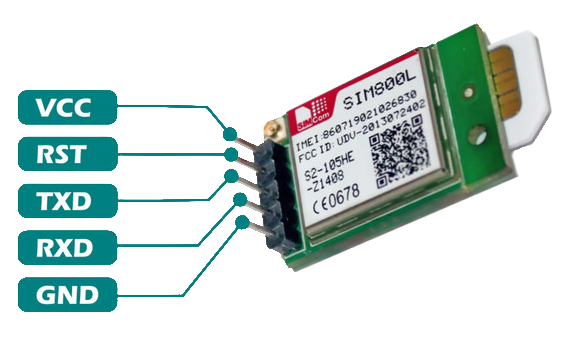
\includegraphics[width=\linewidth,height=2.08333in,keepaspectratio]{images/media/22_1_sim800L.png}

}

\subcaption{\textbf{Figure 22.1. }4V SIM800L green PCB.}

\end{figure}%

\end{minipage}%
%
\begin{minipage}{0.33\linewidth}

\begin{figure}[H]

{\centering 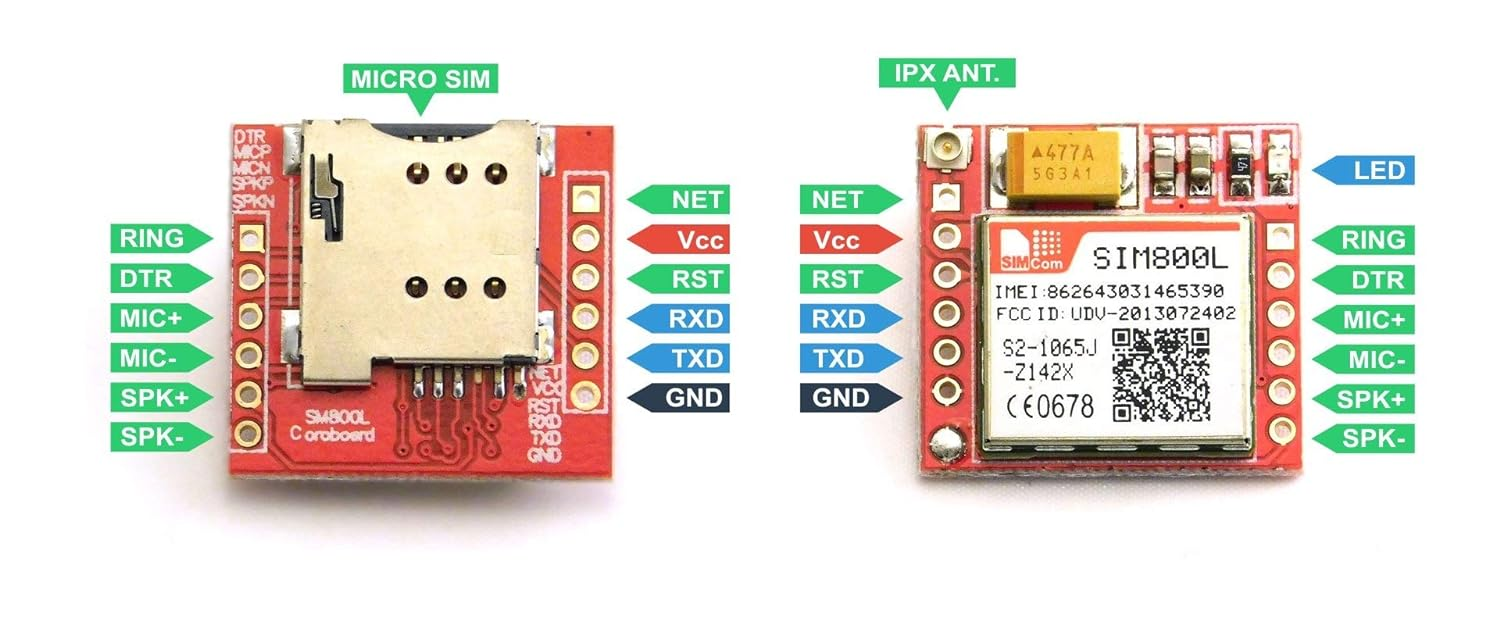
\includegraphics[width=5in,height=2.08333in]{images/media/22_2_sim800L.jpeg}

}

\subcaption{\textbf{Figure 22.2. }4V SIM800L red PCB.}

\end{figure}%

\end{minipage}%
%
\begin{minipage}{0.33\linewidth}

\begin{figure}[H]

{\centering 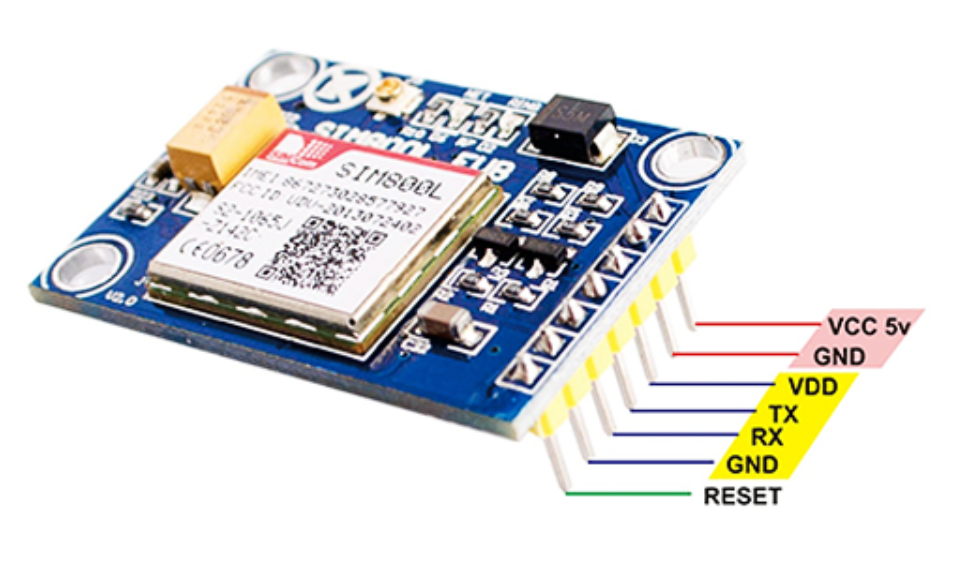
\includegraphics[width=\linewidth,height=2.08333in,keepaspectratio]{images/media/22_3_sim800L-v2.png}

}

\subcaption{\textbf{Figure 22.3. }5V SIM800L-v2.}

\end{figure}%

\end{minipage}%

\end{figure}%

An adapter board can be made, or the Monitor PCB modified, if a green
module at the first three sites ever needs to be replaced with a red
one.

Install the SIM800L Module header in the top left section of the board,
as the module needs to be located close to the antenna slot on the
mounting bracket (see fig.~23).

Use female header pins to create a socket for the module. This enables
the module to be easily removed for testing or to be replaced if faulty.

\begin{itemize}
\item
  Install capacitors C1 -- C4 and Zener diode D1.
\item
  With the SIM800L/SIM800L-v2 \textbf{NOT} inserted, confirm on the
  header that there is 4.0 V between VCC and GND, or 5.0 V if using the
  SIM800L-v2.
\end{itemize}

\begin{figure}[H]

{\centering 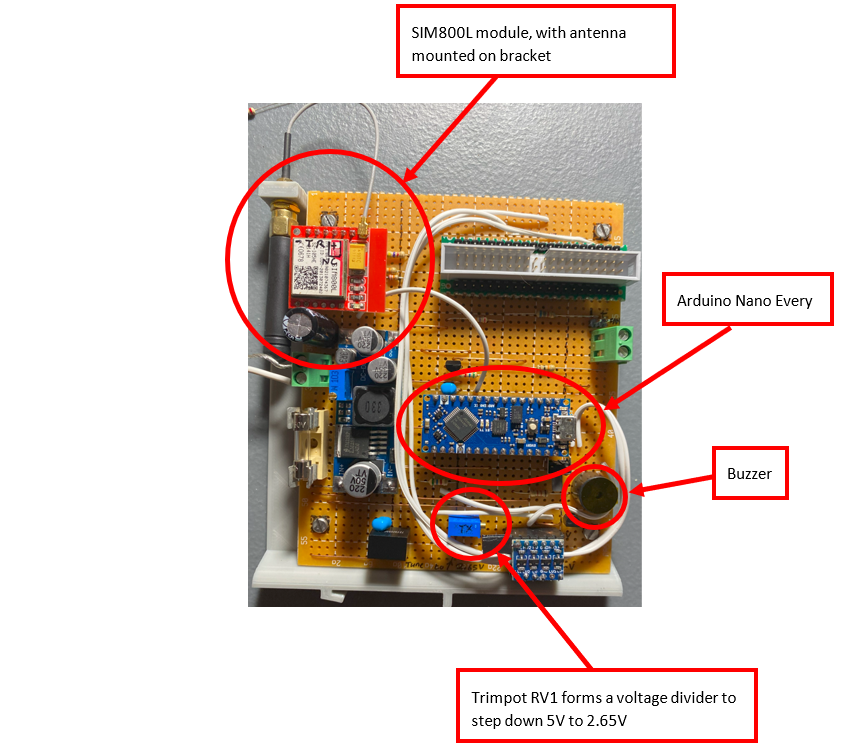
\includegraphics[width=4.16667in,height=\textheight,keepaspectratio]{images/media/23_monitor.png}

}

\caption{\textbf{Figure 23.} Robben Island APMS monitor board.}

\end{figure}%

\subsection{Communication Between SIM800L and
Arduino}\label{communication-between-sim800l-and-arduino}

\begin{itemize}
\tightlist
\item
  \ul{SIM800L RX and Arduino TX}
\end{itemize}

Since the TX of the Arduino is between 0V and 5V, a simple voltage
divider is used to step the voltage down to a level suitable for the
SIM800L. Install Trimpot RV1 as per the schematic.

With the SIM800L module and Arduino \ul{not} inserted, apply 5V to the
voltage divider (pin D3 -- See FIGURE 24 - ARDUINO NANO PINOUT). With 5V
applied to D3, a voltage divider is created by trimpot RV1. Adjust the
trimpot until the voltage on the centre pin, is 2.65 V. This pin will be
connected to the receive line of the SIM800L.

\begin{itemize}
\tightlist
\item
  \ul{SIM800L TX and Arduino RX}
\end{itemize}

The voltage level of the SIM800L needs to be stepped up for use with the
Arduino. To achieve this, a circuit consisting of three resistors (R8,
R9 and R10) and one NPN transistor (Q1) is used, as recommended by the
SIM800L manual. Install the above-mentioned resistors and transistors
and ensure the input of the circuit is connected to the transmit line of
the SIM800L.

\subsection{Communication Between SIM800L-V2 and
Arduino}\label{communication-between-sim800l-v2-and-arduino}

\begin{itemize}
\tightlist
\item
  \ul{SIM800L-V2 RX and Arduino TX}
\end{itemize}

To be completed.

\begin{itemize}
\tightlist
\item
  \ul{SIM800L-V2 TX and Arduino RX}
\end{itemize}

To be completed.

\begin{figure}[H]

{\centering 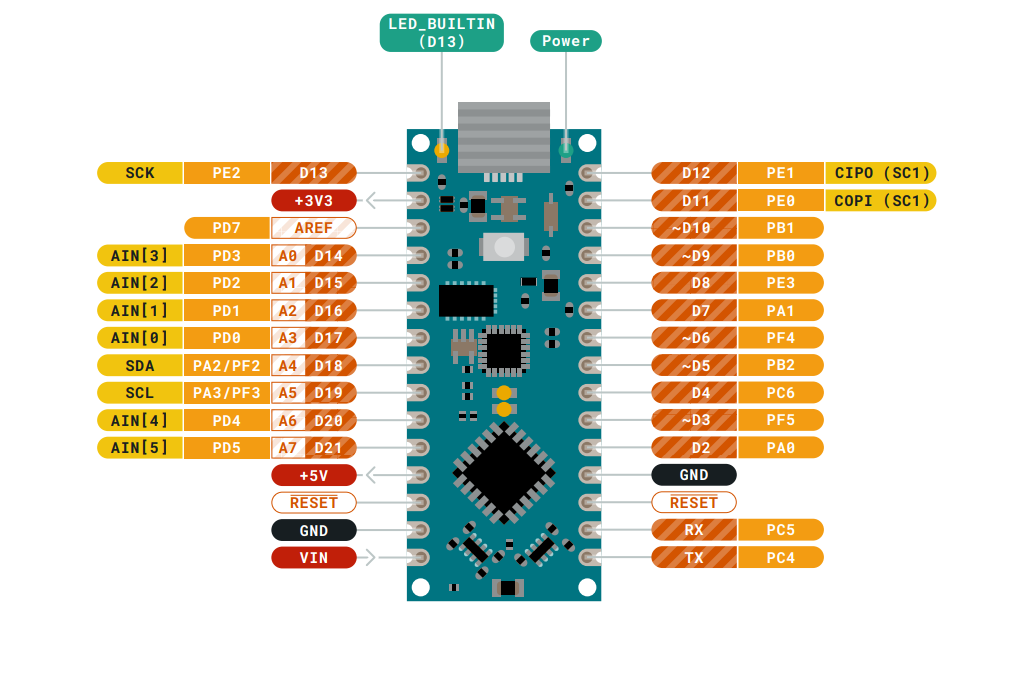
\includegraphics[width=6.25in,height=\textheight,keepaspectratio]{images/media/24_arduino_pinout.png}

}

\caption{\textbf{Figure 24.} Arduino Nano pinout.}

\end{figure}%

\subsection{Raspberry Pi Connection}\label{raspberry-pi-connection}

The connector used to connect the Monitor to the Raspberry Pi can be
seen in fig.~25. To use the connector with stripboard, the pins must
either be bent outwards, or a ``breakout'' board made from a piece of
scrap protoboard (fig.~26). Both methods have been used and are
effective. A pre-made break-out board can be purchased if available. If
a PCB is designed in future, it will be possible to solder the connector
directly on the board.

\begin{figure}

\begin{minipage}{0.50\linewidth}

\begin{figure}[H]

{\centering 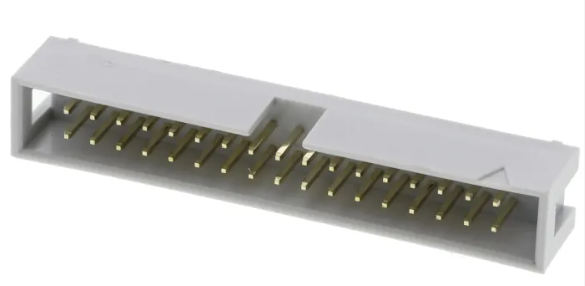
\includegraphics[width=4.16667in,height=\textheight,keepaspectratio]{images/media/25_connector.png}

}

\subcaption{\textbf{Figure 25.} Raspberry Pi connector.}

\end{figure}%

\end{minipage}%
%
\begin{minipage}{0.50\linewidth}

\begin{figure}[H]

{\centering 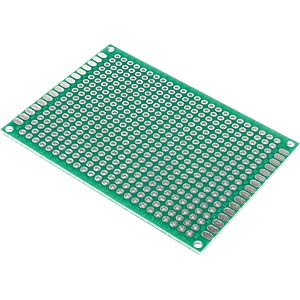
\includegraphics[width=4.16667in,height=\textheight,keepaspectratio]{images/media/26_protoboard.jpeg}

}

\subcaption{\textbf{Figure 26.} Proto board.}

\end{figure}%

\end{minipage}%

\end{figure}%

The Raspberry Pi 40-pin Connector pinout can be seen in fig.~27.

A simple voltage check of 3.3V on pin 1 and 5V pin 2 should confirm
orientation if unsure.

The Raspberry Pi GPIO pins and their functions can be seen in TABLE 3 -
RASPBERRY PI GPIO PINS AND FUNCTIONS

\begin{figure}[H]

{\centering 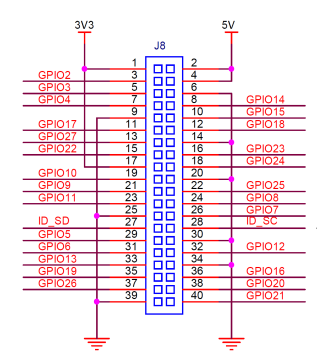
\includegraphics[width=4.16667in,height=\textheight,keepaspectratio]{images/media/27_pi_pinout.png}

}

\caption{\textbf{Figure 27.} Raspberry Pi GPIO pinout.}

\end{figure}%

\begin{longtable}[]{@{}
  >{\raggedright\arraybackslash}p{(\linewidth - 2\tabcolsep) * \real{0.3108}}
  >{\raggedright\arraybackslash}p{(\linewidth - 2\tabcolsep) * \real{0.6622}}@{}}
\caption{\textbf{Table 3} - Raspberry Pi GPIO pins and
functions}\tabularnewline
\toprule\noalign{}
\begin{minipage}[b]{\linewidth}\raggedright
Pin
\end{minipage} & \begin{minipage}[b]{\linewidth}\raggedright
Function
\end{minipage} \\
\midrule\noalign{}
\endfirsthead
\toprule\noalign{}
\begin{minipage}[b]{\linewidth}\raggedright
Pin
\end{minipage} & \begin{minipage}[b]{\linewidth}\raggedright
Function
\end{minipage} \\
\midrule\noalign{}
\endhead
\bottomrule\noalign{}
\endlastfoot
GPIO3 & Power ON/OFF \\
GPIO4 & Raspberry Pi UART3 TX \\
GPIO5 & Raspberry Pi UART3 RX \\
GPIO14 & Raspberry Pi TX \\
GPIO15 & Raspberry Pi RX \\
\end{longtable}

\begin{figure}[H]

{\centering 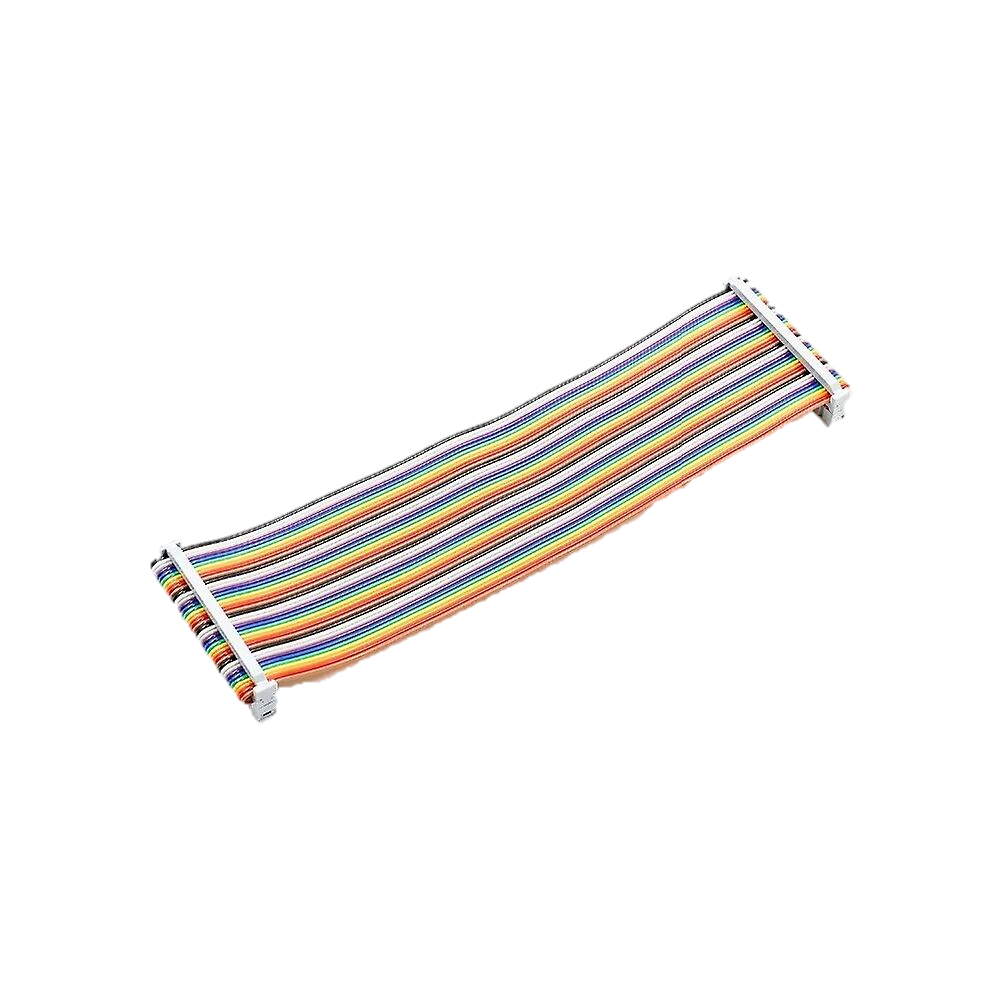
\includegraphics[width=4.16667in,height=\textheight,keepaspectratio]{images/media/28_ribbon.png}

}

\caption{\textbf{Figure 28.} 40 pin ribbon cable.}

\end{figure}%

A 40-pin ribbon cable is used to connect the Monitor to the Raspberry Pi
(fig.~28). After building the Monitor, \textbf{check the voltages on the
other end of the ribbon cable, to ensure it is not above 3.3V, before
plugging it into the Pi}.

\subsection{Logic Level Shifter}\label{logic-level-shifter}

\begin{itemize}
\item
  Since the Pi uses 3.3 V for communication, and the Arduino 5 V, a
  logic level shifter is needed. These modules are available cheaply and
  two 6-pin female headers should be used as a socket for easy
  install/removal (fig.~29).
\item
  The level shifter uses the 3.3V on pin 1 of the Raspberry Pi connector
  for the LV connection and the 5V Arduino supply voltage for the HV
  connection.
\end{itemize}

\begin{figure}[H]

{\centering 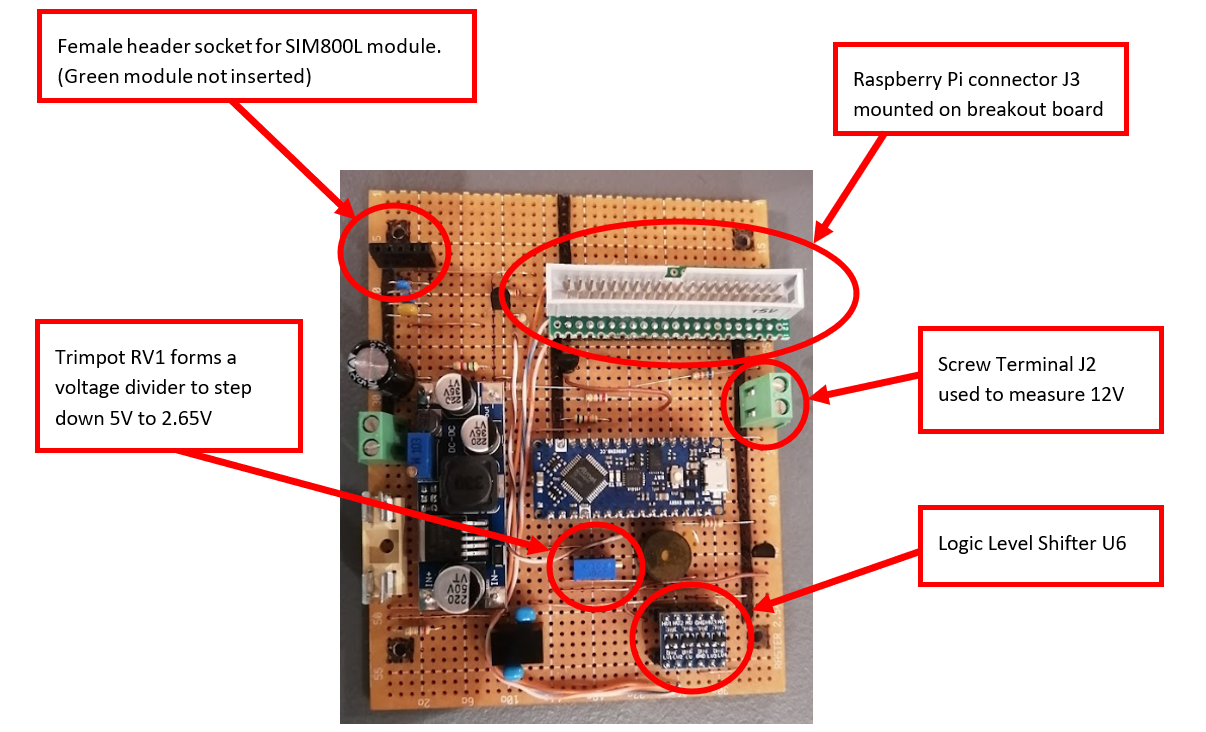
\includegraphics[width=6.25in,height=\textheight,keepaspectratio]{images/media/29_dyer_monitor.png}

}

\caption{\textbf{Figure 29.} Dyer Island monitor board.}

\end{figure}%

\subsection{UPDI Programming}\label{updi-programming}

The Arduino Nano Every uses UPDI (Unified Program and Debug Interface)
for programming. This uses only 1 wire for programming, but a more
complex communication protocol is needed. To use UPDI a wire needs to be
soldered to a pad located on the underside of the Arduino. A link must
also be soldered (Fig. 30).

\textbf{NOTE: After the link has been made, the board can no longer be
programmed via the Arduino software and USB cable. It will be programmed
via the Raspberry Pi using the UPDI wire. If the Arduino software needs
to be used during fault finding, unsolder the link. The pads can break
off with successive heating sessions, so be cautious.}

\begin{figure}[H]

{\centering 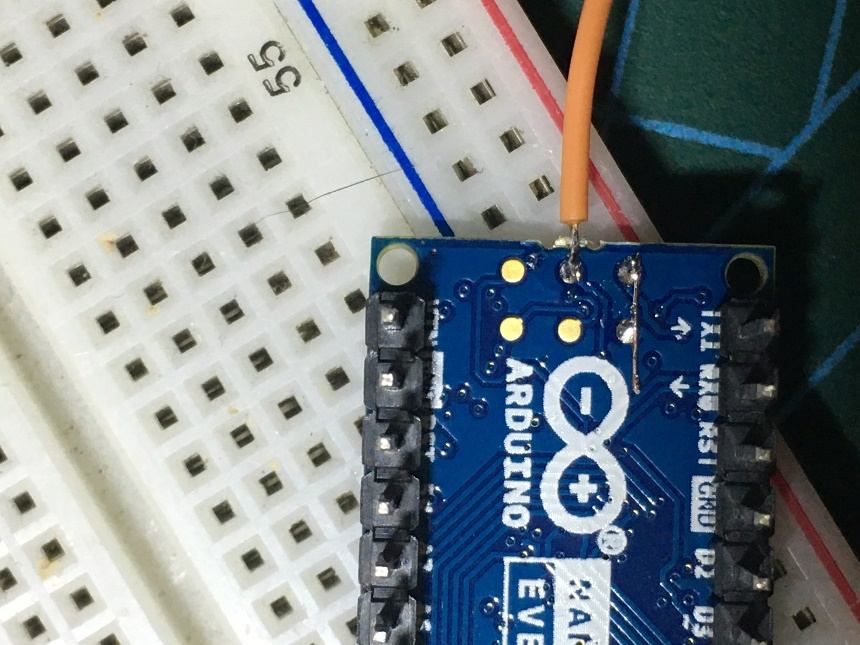
\includegraphics[width=4.16667in,height=\textheight,keepaspectratio]{images/media/30_updi_arduino.jpeg}

}

\caption{\textbf{Figure 30.} Wire and link soldered onto Arduino for
UPDI programming.}

\end{figure}%

\begin{itemize}
\item
  To program the Arduino remotely via the Raspberry Pi, a utility called
  ``pymcuprog'' is used. This utility allows the Raspberry Pi to program
  the Arduino via a serial connection. This serial connection is
  established using UART3 (RX3 and TX3) on the Raspberry Pi as a serial
  port (see Table 3 for GPIO pinout).
\item
  To program the Arduino via a serial port, a hardware modification is
  required. The pymcuprog documentation
  (\url{https://pypi.org/project/pymcuprog/}) describes various
  combinations of diodes and resistors to achieve this, for various
  setups. After experimentation, using only a Schottky diode (D2)
  delivered the best results. Note the cathode of D2 is connected to
  TX3.
\item
  The UPDI wire is connected to HV1 on the level shifter (Fig. 18).
\item
  A script has been written to compile and upload the firmware to the
  Arduino, from the Raspberry Pi, thus the user does not need to use
  pymcuprog directly. See the section: PROGRAMMING THE ARDUINO MONITOR
  VIA THE PI.
\end{itemize}

\subsection{Voltage Monitoring}\label{voltage-monitoring}

If any of the main supply voltages are outside allowable limits, an SMS
will be sent to the operator.

Currently, the following important voltages are monitored:

\begin{itemize}
\tightlist
\item
  4V: This is the SIM800L supply voltage. This voltage is generated by
  the LM2596 voltage regulator and is fed to analog input A6 of the
  Arduino, via resistor R1.
\end{itemize}

\begin{quote}
Note: In version 2 of the monitor board a different SIM module is used
which no longer needs a 4V supply voltage. As a result this is no longer
monitored.
\end{quote}

\begin{itemize}
\tightlist
\item
  5V: This is the 5V supply for the Raspberry Pi. The 5V is picked up
  from pin 2 or 4 on the Raspberry Pi connector (See Fig. 27 for the
  Raspberry Pi GPIO pinout).
\end{itemize}

\begin{quote}
Note: As this voltage is close to, and might exceed, the Arduino maximum
safe voltage, a voltage divider consisting of R2 and R3 is used to step
the voltage down. The Arduino uses A3 to measure this voltage. Note that
this 5V is separate and should be isolated from the Arduino 5V supply.
This is in essence measuring the output of the 5V Meanwell Power Supply.
\end{quote}

\begin{itemize}
\item
  12V: This is the 12V supply for the scales and the router (if an
  indoor router is used). This voltage is fed via a wire from the
  Meanwell 12V Power Supply to screw terminal J2. Install the screw
  terminal in the top right section of the board to allow for easy
  connecting when installing the board (Fig. 29). Resistor R4 and R5 is
  used to step the 12V before connecting it to A5 of the Arduino
\item
  24V: This is the main solar supply voltage. This supplies power to the
  BioMark reader, the APMS Main Unit and the Outdoor Router (if one is
  installed). The voltage is measured at the input of the Monitor and is
  stepped down via resistor divider R6 and R7 before being connected to
  A7 of the Arduino.
\end{itemize}

\subsection{Temperature Monitoring}\label{temperature-monitoring}

The ambient temperature inside the Main Unit is monitored using a LM35
temperature sensor (U5). The sensor operates on 5V and needs no other
components to operate. The output of the sensor is read directly by
analog pin A0 on the Arduino.

\subsection{Buzzer and Button}\label{buzzer-and-button}

A buzzer and button are included for debugging and future options.
Currently the Monitor will beep once initialisation is complete, and the
button will power the Raspberry Pi down/up.

\begin{itemize}
\item
  The buzzer is switched via transistor Q2 with base current being
  limited by resistor R11.
\item
  The button is connected directly to pin D12 on the Arduino and makes
  use of the built-in pull-up resistor, thus requiring no other
  components. Place the button on the board in a location where it will
  be easy to press once the board is installed.
\end{itemize}

\subsection{Testing the Monitor Circuit
Board}\label{testing-the-monitor-circuit-board}

Before testing communication between the Raspberry Pi and the Arduino
Monitor, some basic tests must be done to ensure no components will be
damaged. A dual variable power supply will be needed to test the various
voltages.

Ensure the firmware was uploaded successfully as explained in the
section PROGRAMMING VIA THE ARDUINO SOFTWARE

Plug the SIM800L into its socket and connect the antenna.

\begin{itemize}
\item
  Plug the Arduino into its socket.
\item
  Plug the Level Shifter into its socket.
\item
  Plug the 40-pin ribbon cable into the socket on the Monitor but do not
  plug the other end into the Pi.
\item
  Power the Monitor via the main 24V DC connector.
\item
  Observe lights flashing on the SIM800L.

  \begin{itemize}
  \tightlist
  \item
    The green light on the SIM800L should flash rapidly at first, and
    after about 20 seconds, it should start flashing slowly. This
    indicates that the module was able to connect to the cell network
    successfully. Try different antennas and orientations for best
    results.
  \end{itemize}
\item
  Check that there is 5.0V on the Arduino and Level Shifter supply pins.
\item
  Check that there is 4.0V on the SIM800L supply pin.

  \begin{itemize}
  \tightlist
  \item
    Check that the same 4.0V is measured on pin A6 of the Arduino.
  \end{itemize}
\item
  Check that none of the pins on the Raspberry Pi connector has 5V on
  it.

  \begin{itemize}
  \tightlist
  \item
    Note pin 2 and 4 will have 5V coming from the Pi when it is
    connected at a later stage.
  \end{itemize}
\item
  Supply 12V to connector J2 and ensure the voltage has dropped to below
  5V on pin A5 of the Arduino.
\item
  Measure the stepped-down solar supply voltage on pin A7 of the
  Arduino. The 24V should have been stepped down to a value less than
  5V.
\item
  Measure the output voltage of the temperature sensor on pin A0 of the
  Arduino. The sensor outputs 10mV per °C, so at 25°C, the voltage
  should be about 0.25V.
\end{itemize}

\chapter{APMS Main Unit}\label{apms-main-unit}

The APMS Main Unit consists of all the electronics needed for the
system.

For a complete parts list, see Table 4.

For a system diagram, see Fig. 31.

\begin{longtable}[]{@{}
  >{\raggedright\arraybackslash}p{(\linewidth - 6\tabcolsep) * \real{0.2561}}
  >{\raggedright\arraybackslash}p{(\linewidth - 6\tabcolsep) * \real{0.1829}}
  >{\raggedright\arraybackslash}p{(\linewidth - 6\tabcolsep) * \real{0.3780}}
  >{\raggedright\arraybackslash}p{(\linewidth - 6\tabcolsep) * \real{0.1585}}@{}}
\caption{Table 4 - APMS Main Unit Parts List}\tabularnewline
\toprule\noalign{}
\begin{minipage}[b]{\linewidth}\raggedright
\textbf{Name}
\end{minipage} & \begin{minipage}[b]{\linewidth}\raggedright
\textbf{Quantity}
\end{minipage} & \begin{minipage}[b]{\linewidth}\raggedright
\textbf{Description}
\end{minipage} & \begin{minipage}[b]{\linewidth}\raggedright
\textbf{RS Part Number}
\end{minipage} \\
\midrule\noalign{}
\endfirsthead
\toprule\noalign{}
\begin{minipage}[b]{\linewidth}\raggedright
\textbf{Name}
\end{minipage} & \begin{minipage}[b]{\linewidth}\raggedright
\textbf{Quantity}
\end{minipage} & \begin{minipage}[b]{\linewidth}\raggedright
\textbf{Description}
\end{minipage} & \begin{minipage}[b]{\linewidth}\raggedright
\textbf{RS Part Number}
\end{minipage} \\
\midrule\noalign{}
\endhead
\bottomrule\noalign{}
\endlastfoot
Enclosure & 1 & Housing for the APMS system & 508-2798 \\
DIN Rail & 1 & DIN rail for mounting electronics & 188-2538 \\
DC 30V 5A Socket & 1 & DC panel socket for main 24V solar input voltage
& 705-1525 \\
DC 30V 5A Plug & 1 & For cable coming from 24V Solar Supply &
705-1519 \\
USB panel mount socket & 1 & To connect to BioMark Reader & 111-6761 \\
DC panel socket (12V 1A) & 1 & 12V output for LTE Router & 111-3725 \\
DC 12V 1A Plug & 1 & Plug for Indoor Router & 138-9405 \\
6-pin socket & 2 & Sockets for scales & 111-5764 \\
6-pin Plug & 2 & Plugs for scales & 111-5758 \\
USB Cable & 1 & Mini USB cable to connect to BioMark Reader &
822-3226 \\
12V 30W PSU & 1 & 12V Power Supply for Router and scales & 175-7778 \\
5V 15W PSU & 1 & 5V Power Supply for Raspberry Pi & 175-7775 \\
Fuse Holder & 1 & Fuse holder & 501-871 \\
3A Fuse & 1 & Main Fuse & 668-5963 \\
USB-RS485 Converter & 2 & USB to RS485 converter & 687-7834 \\
64GB SD Card & 1 & Main storage for APMS operating system. & Takealot \\
64GB USB Flash drive & 1 & USB Flash drive for data backup & Takealot \\
Raspberry Pi 4 & 1 & Main computer for APMS system & 182-2096 \\
Heatsinks & 3 & For cooling Raspberry Pi processors & 201-2169 \\
Fan & 1 & For cooling Raspberry Pi processors & 789-7858 \\
2-pin Female Header for Fan & 1 & Same as used for APMS Monitor &
767-9842 \\
USB-C cable for power & 1 & Cabe for powering Raspberry Pi & 192-4730 \\
Mount for Raspberry Pi & 1 & 3D Printed DIN Rail Mount for Raspberry Pi
& Printed in-house \\
Mount for Arduino Monitor & 1 & 3D Printed DIN Rail Mount for APMS
Monitor & Printed in-house \\
3D Printed Fan Mount & 1 & To mount the cooling fan above the CPU &
Printed in-house \\
Monitor Board & 1 & Used to monitor health of main system & Built
in-house \\
SIM card & 2 & Sim card for main system and monitor board & Vodacom
shop \\
Internal wiring & & Used for various connections inside box & Hardware
store \\
Ferrules & & For better contact with screw terminals & Takealot \\
Heat-shrink & & Insulate connections & Takealot \\
M2.5x8 machine screws & 4 & Screws to secure the Raspberry Pi &
914-1567 \\
M3x16 machine screws & 4 & Screws to secure the fan & 190-462 \\
\end{longtable}

\begin{figure}[H]

{\centering 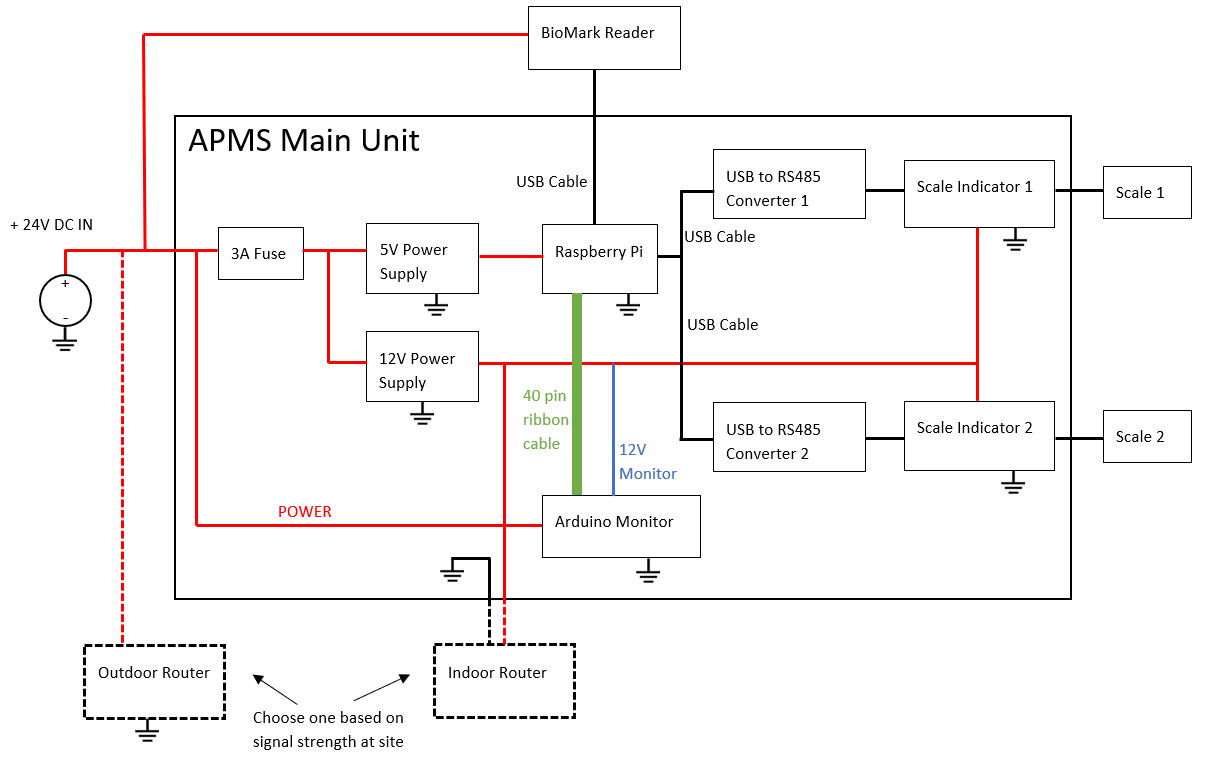
\includegraphics[width=6.25in,height=\textheight,keepaspectratio]{images/media/31_apms_diagram.png}

}

\caption{\textbf{Figure 31.} APMS system diagram.}

\end{figure}%

\section{Preparing the USB Panel Mount
Socket}\label{preparing-the-usb-panel-mount-socket}

The USB Panel Mount Socket does not have adequate strain relief. Use
Pratley Putty to reinforce the cables. Take note to avoid getting the
putty on the threads (Fig. 32).

\begin{figure}[H]

{\centering 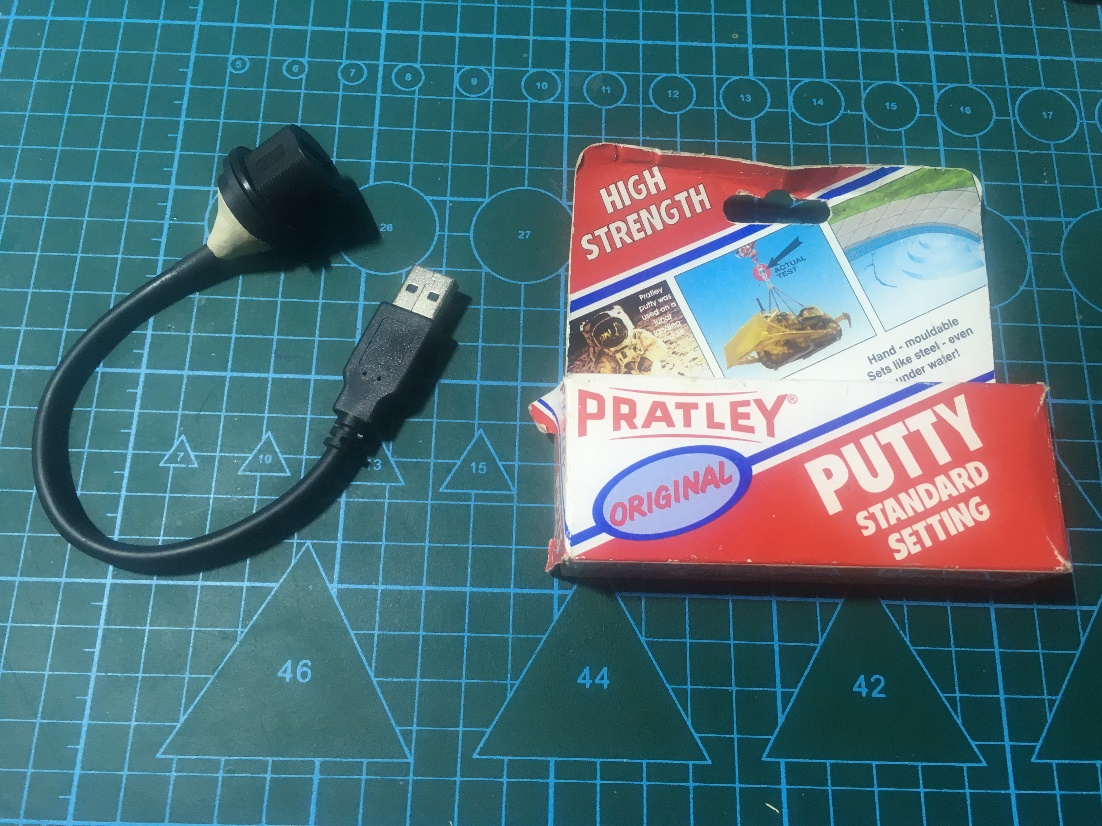
\includegraphics[width=6.25in,height=\textheight,keepaspectratio]{images/media/32_1_pratley_socket.jpeg}

}

\caption{\textbf{Figure 32.1.} Pratley putty strain relief for USB
socket.}

\end{figure}%

\begin{figure}[H]

{\centering 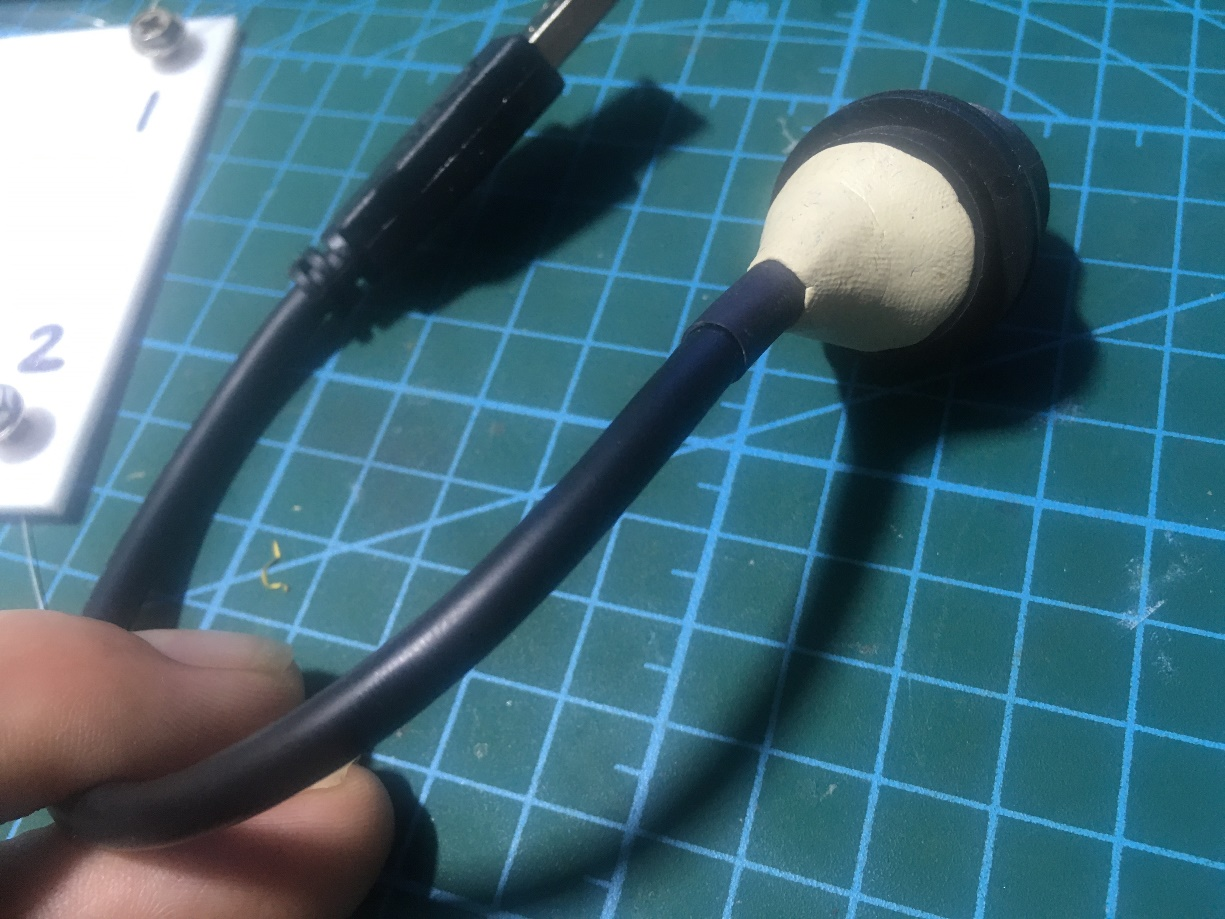
\includegraphics[width=4.16667in,height=\textheight,keepaspectratio]{images/media/32_2_pratley_socket.jpeg}

}

\caption{\textbf{Figure 32.2. }Pratley putty strain relief for USB
socket.}

\end{figure}%

\section{Preparing the Main Unit
Enclosure}\label{preparing-the-main-unit-enclosure}

Prepare the enclosure before starting the build. RS Part numbers
included in brackets.

\begin{itemize}
\item
  Open the enclosure (508-2798) and screw down the DIN rail (188-2538)
  using the screws provided. Note, it takes a fair bit of force.
\item
  Download and print the template here:
  \href{images/media/apms_template_v1.2.pdf}{Download APMS template}.
  Check the dimensions with a ruler after printing.
\item
  Glue/stick the template on to the front of the enclosure and drill the
  holes as indicated on the template.

  \begin{itemize}
  \tightlist
  \item
    The 11mm and 21mm diameter holes are an odd size. Either go one size
    smaller and enlarge, or use one size larger, with it being a
    slightly loose fit.
  \end{itemize}
\item
  Do a test fit of all the sockets:

  \begin{itemize}
  \tightlist
  \item
    Main DC socket (705-1525),
  \item
    USB Panel Mount Socket (111-6761),
  \item
    12V DC socket (111-3725), and
  \item
    two scale sockets (111-5764)
  \end{itemize}
\item
  The sockets can be removed to ease in the rest of the build.
\item
  Use a label maker, or a permanent marker, and label each socket (Fig.
  33).
\end{itemize}

\begin{figure}[H]

{\centering 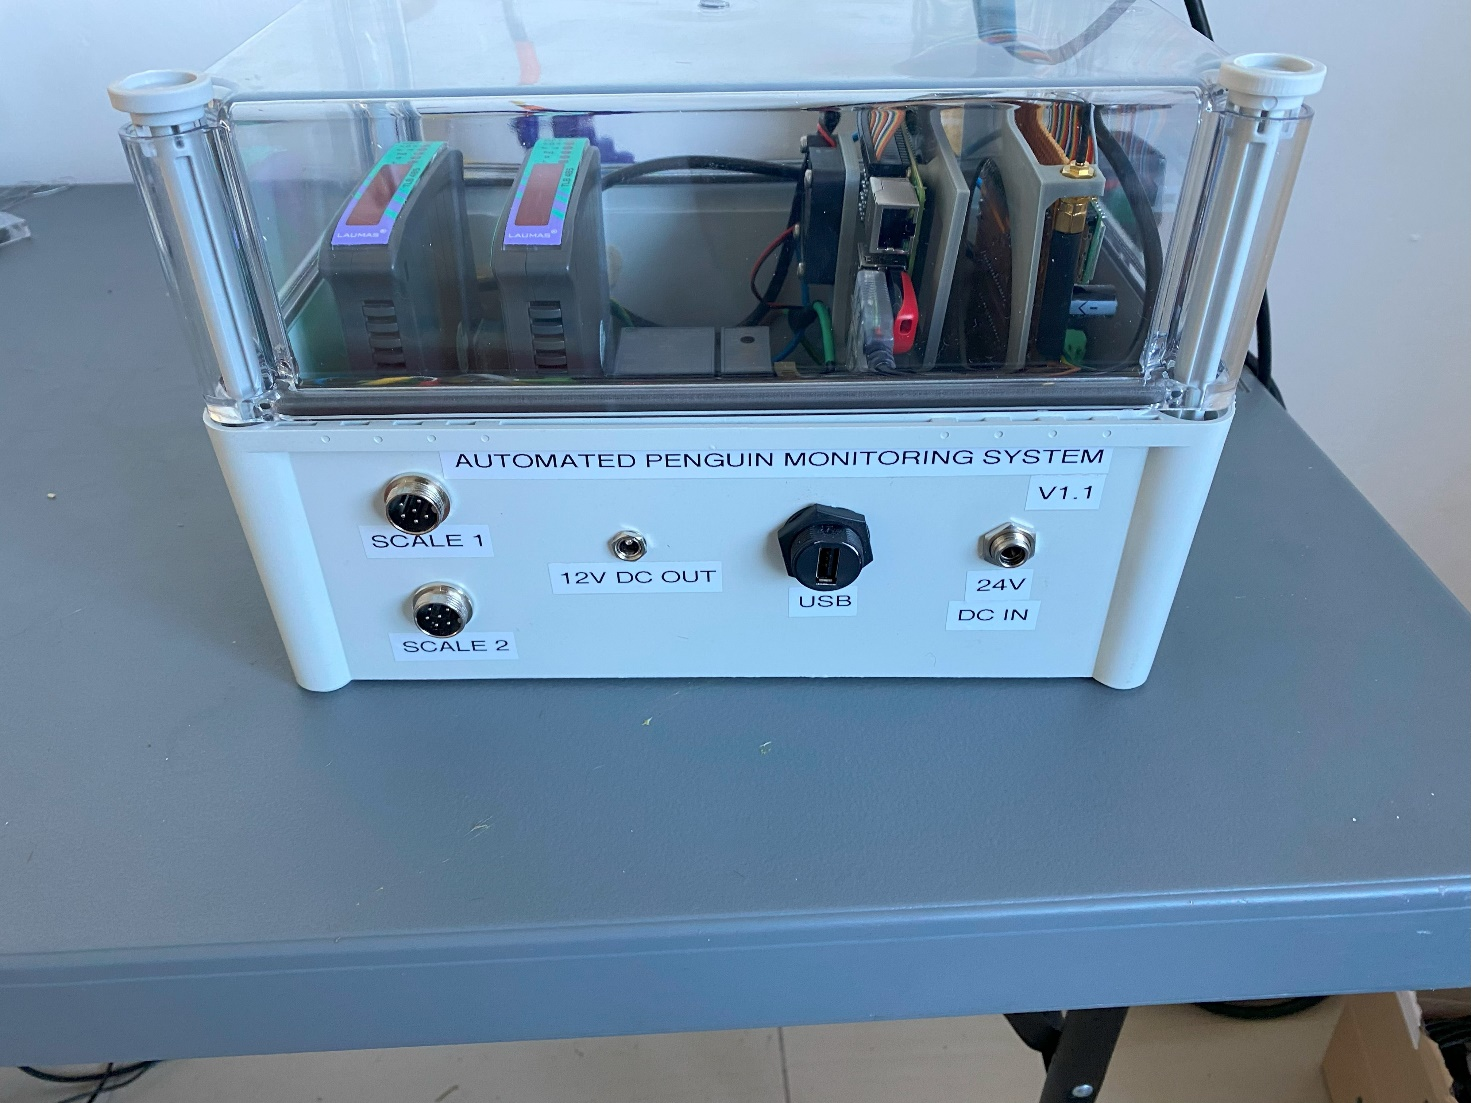
\includegraphics[width=4.16667in,height=\textheight,keepaspectratio]{images/media/33_apms_front.jpeg}

}

\caption{\textbf{Figure 33.} APMS Main Unit frontside.}

\end{figure}%

\begin{tcolorbox}[enhanced jigsaw, left=2mm, toptitle=1mm, breakable, opacitybacktitle=0.6, title=\textcolor{quarto-callout-note-color}{\faInfo}\hspace{0.5em}{Note}, colback=white, opacityback=0, rightrule=.15mm, leftrule=.75mm, colbacktitle=quarto-callout-note-color!10!white, bottomtitle=1mm, titlerule=0mm, coltitle=black, colframe=quarto-callout-note-color-frame, arc=.35mm, bottomrule=.15mm, toprule=.15mm]

There are now two versions of the APMS.

In \textbf{version 1.1} the following improvements were made:

\begin{itemize}
\tightlist
\item
  More robust fan with newly designed fan bracket
\item
  Use of RS485 converters, instead of RS232
\item
  Scales are mounted on marine ply, instead of inside boxes
\end{itemize}

In \textbf{version 1.2} the following improvements were made:

\begin{itemize}
\tightlist
\item
  New APMS Main Unit enclosure that is easier to open
\item
  New SIM800L-V2 module that has an integrated power supply unit and
  doesn't need the power to be converted to 4V anymore.
\item
  New Teltonika RUT906/RUT956 routers which allow remote calibration and
  taring of scales and extendable SMA cable ports for better cellphone
  reception.
\item
  New scale indicators (General Measure GMT-X1) which allow RS485
  connection and management capabilities.
\item
  Tailor-made, custom BioMark RFID antennas to fit perfectly between the
  two scales. This design makes the antenna much easier to tune and
  protects the cable from being accidentally kicked out of place (which
  previously caused a loss of resonance). Additionally, these commercial
  antennas offer a significantly stronger detection range than the
  legacy homemade versions.
\end{itemize}

\end{tcolorbox}

\section{Mounting The Raspberry Pi}\label{mounting-the-raspberry-pi}

Use four 2.5mm machine screws to mount the Raspberry Pi on the mounting
plate (Figs. 34 and 35).

Add heatsinks (RS: 201-2169) (Fig. 35)

\begin{figure}[H]

{\centering 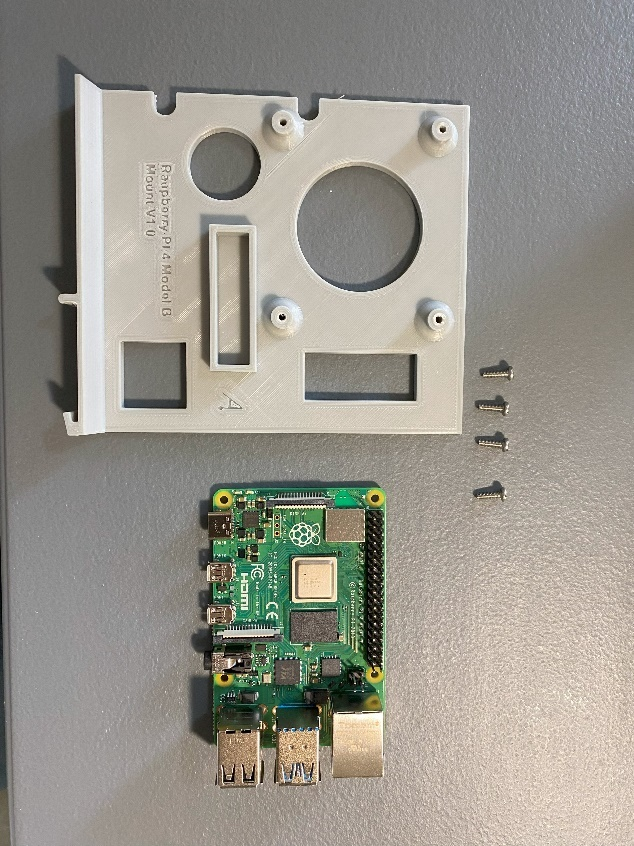
\includegraphics[width=4.16667in,height=\textheight,keepaspectratio]{images/media/34_pi_mounting.jpeg}

}

\caption{\textbf{Figure 34.} Raspberry Pi 4 with mounting plate.}

\end{figure}%

\begin{figure}[H]

{\centering 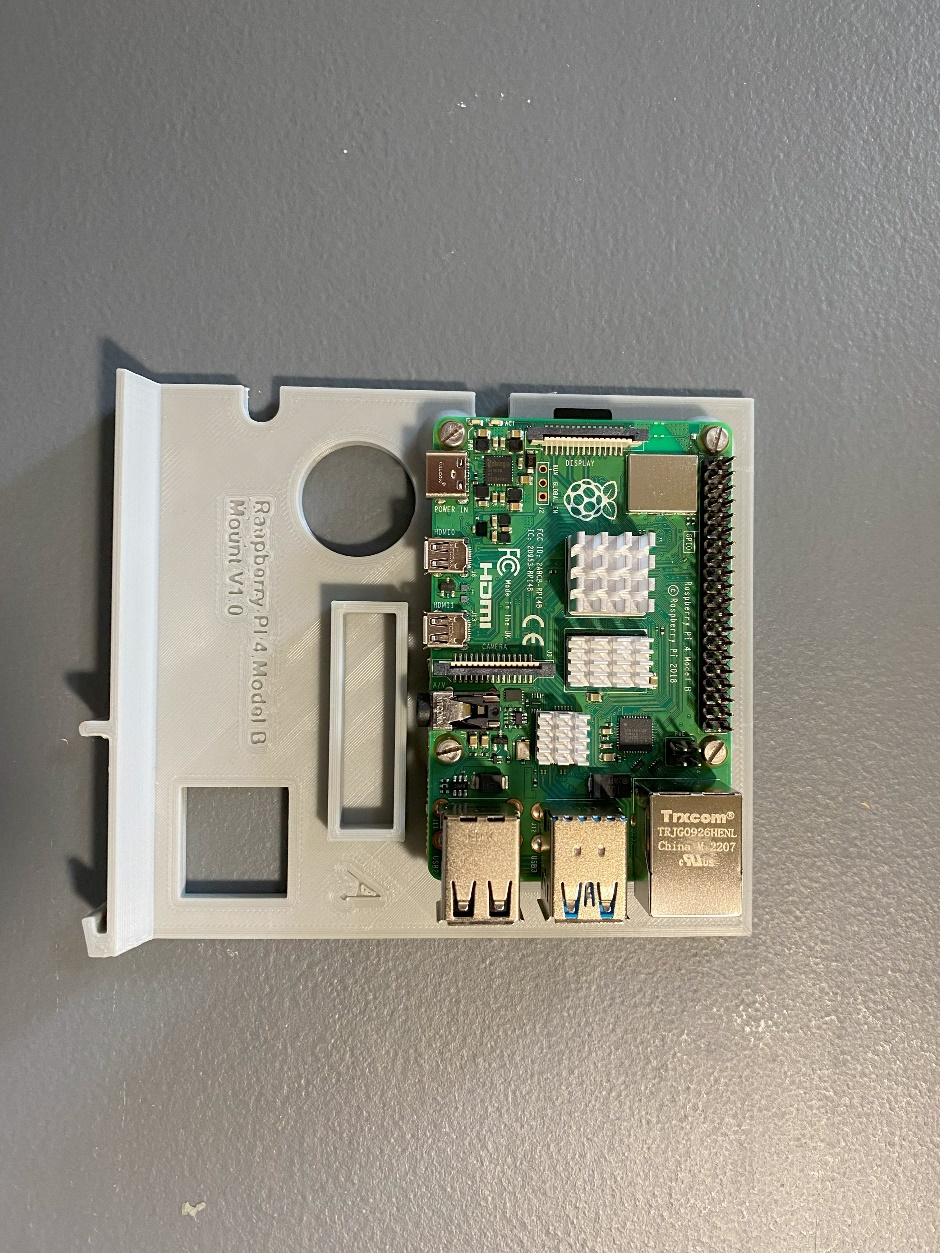
\includegraphics[width=4.16667in,height=\textheight,keepaspectratio]{images/media/35_pi_mounting.jpeg}

}

\caption{\textbf{Figure 35.} Raspberry Pi mounted with heatsinks.}

\end{figure}%

\section{Preparing the Fan}\label{preparing-the-fan}

Solder a 2-pin female header connector to the ends of fan cable. Use the
four M3 screws and mount the fan to the fan bracket (Fig. 36).

\begin{figure}[H]

{\centering 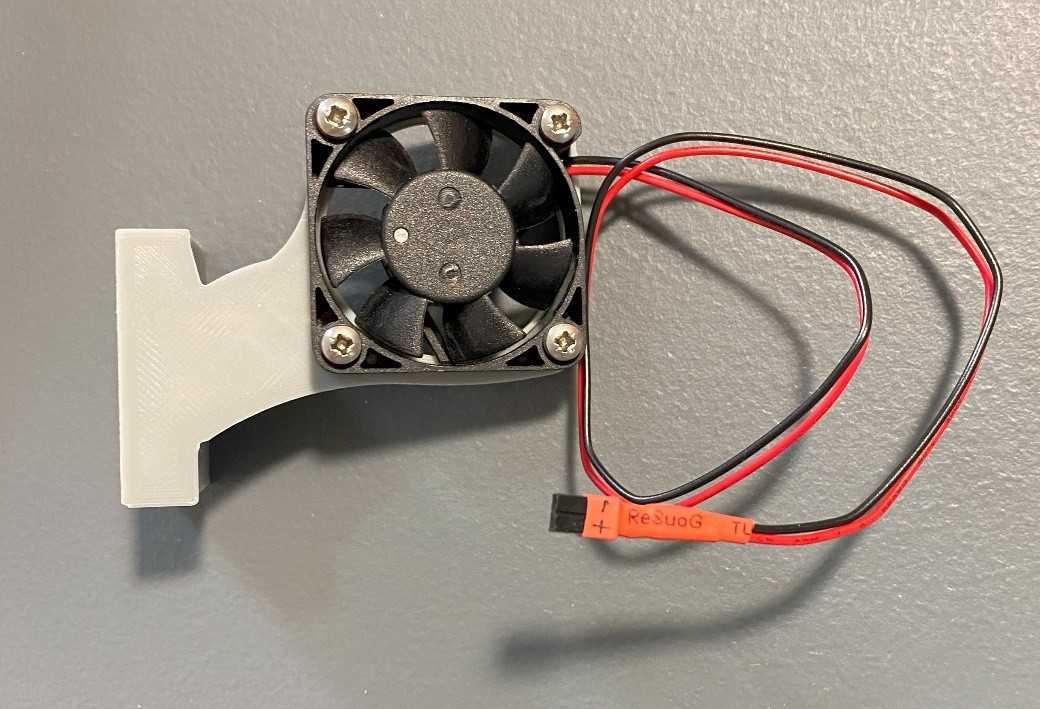
\includegraphics[width=4.16667in,height=\textheight,keepaspectratio]{images/media/36_fan.jpeg}

}

\caption{\textbf{Figure 36} CPU fan mounted on bracket.}

\end{figure}%

The fan and bracket fits into the slot provided on the Raspberry Pi
mounting plate. The fan bracket slides in with a friction fit to allow
easy installation/removal.

\begin{quote}
NOTE: Even though 5V power is provided to the fan from the Monitor, the
5V is retrieved from the Raspberry Pi connector, and not from the 5V
supply on the Monitor itself. This is done to prevent the fan stopping
should the Monitor fail. The fan is connected to pin 4 and 6 on the
Raspberry Pi.
\end{quote}

\section{Wiring the APMS Main Unit}\label{wiring-the-apms-main-unit}

\begin{itemize}
\item
  The location of the DIN mounted components, as well as the power
  wires, can be seen in Fig. 38.
\item
  The main power wires consist of a ground wire, a 5V and a 12V wire.
\item
  The APMS uses a DIN mounted Fuse Holder (501-871) with a 3A Fuse
  (668-5963) to provide protection.
\item
  Two Meanwell Power Supplies are used to step the 24V DC down to the
  required voltages:

  \begin{itemize}
  \item
    5V 15W Power Supply (175-7775) for the Raspberry Pi
  \item
    12V 30W Power Supply (175-7778) for the scales (and indoor router if
    used).
  \end{itemize}
\end{itemize}

\begin{quote}
NOTE the polarity of the two Meanwell power supplies, as they are
opposite to each other.
\end{quote}

\begin{itemize}
\item
  Install the 24V DC and 12V DC connectors.
\item
  Mount the Arduino Monitor, Raspberry Pi, Fuse Holder, 5V Power Supply,
  12V Power Supply and the two Scale Indicators on the DIN Rail.

  \begin{itemize}
  \tightlist
  \item
    If the Arduino Monitor has not been built yet, use the 3D printed
    mounting plate is this step.
  \end{itemize}
\item
  Run a ground wire from the Main 24V DC Connector to the following
  components:

  \begin{itemize}
  \item
    Arduino Monitor
  \item
    Input and Output of 5V Power Supply
  \item
    Input and Output of 12V Power Supply
  \item
    Raspberry Pi
  \item
    Two Scale Indicators
  \item
    12V DC connector
  \end{itemize}
\end{itemize}

\begin{figure}[H]

{\centering 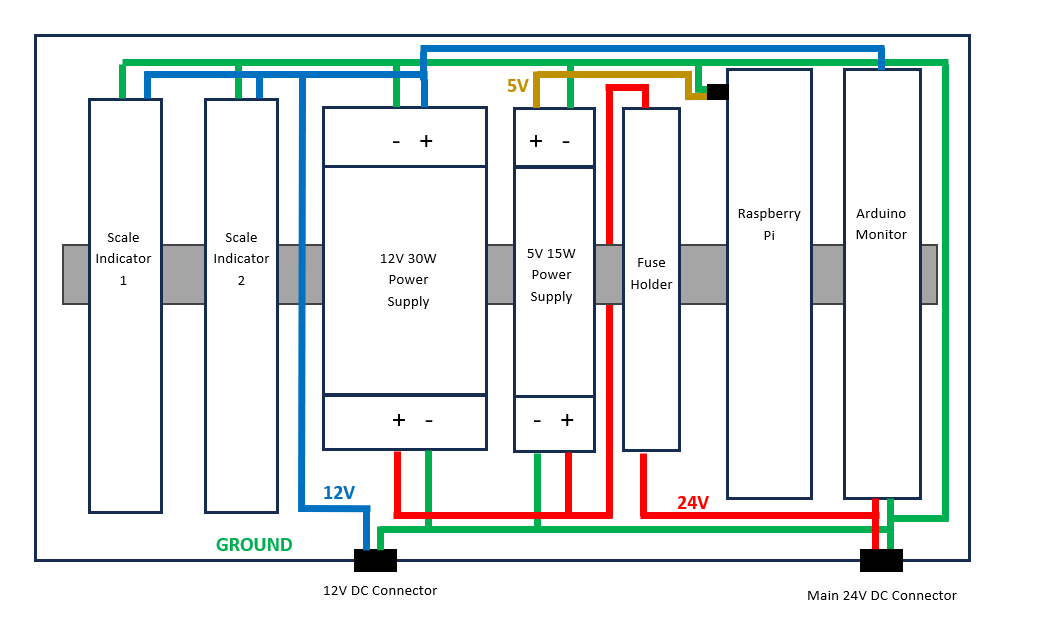
\includegraphics[width=7.29167in,height=\textheight,keepaspectratio]{images/media/39_power_cables.png}

}

\caption{\textbf{Figure 38.} Location of DIN mounted components and
power wires.}

\end{figure}%

\begin{itemize}
\item
  With the ground wire laid out, the locations of the different
  components are established. The Arduino Monitor, Raspberry Pi and the
  two Scale Indicators can now be removed to ease the rest of the
  wiring.
\item
  Run two positive wires from the Main 24 DC Connector:

  \begin{itemize}
  \item
    One through the fuse holder and to the input of the 5V and 12V Power
    Supplies,
  \item
    One to the power connector on the Arduino Monitor.

    \begin{itemize}
    \tightlist
    \item
      The Arduino Monitor has its own 3A fuse. This allows the Monitor
      to continue operating even if a fault caused the main fuse to
      blow.
    \end{itemize}
  \end{itemize}
\item
  On the output of the 5V power supply, run a wire for the Raspberry Pi.
  This positive 5V wire, together with the ground wire created earlier,
  will be connected to a USB-C cable, to power the PI. Currently, the
  most cost-effective method to obtain a quality cable with a USB-C
  connector, is to use a USB-B to USB-C cable from RS Components
  (192-4730) and to cut off the USB-B connector. Please update this
  manual when a better alternative is sourced. Keep the cable running to
  the Pi short to avoid extra cabling in the Main Unit.
\item
  Run a positive 12V wire from the output of the 12V Power supply to the
  following locations:

  \begin{itemize}
  \item
    Arduino Monitor 12V monitoring screw terminal
  \item
    Both Scale Indicators
  \item
    12V DC Socket
  \end{itemize}
\item
  Crimp ferrules to the ends of all the power wires.
\end{itemize}

\begin{figure}[H]

{\centering 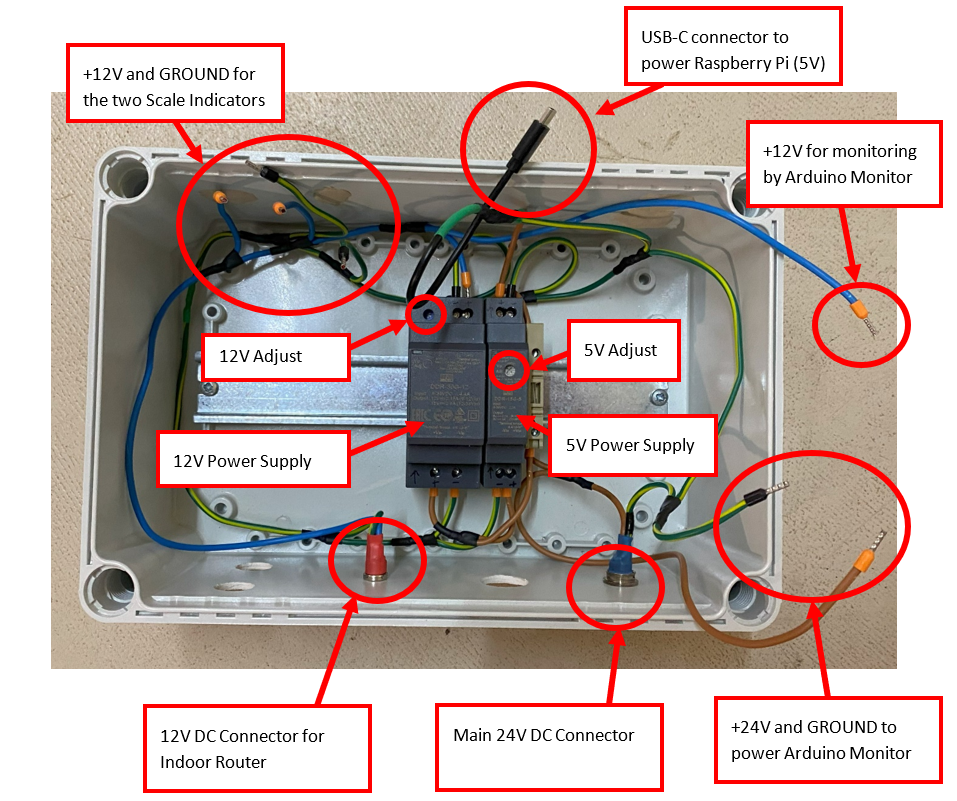
\includegraphics[width=7.29167in,height=\textheight,keepaspectratio]{images/media/40_power_cables_2.png}

}

\caption{\textbf{Figure 40.} Power supplies and wiring.}

\end{figure}%

\section{Testing the Power Supplies}\label{testing-the-power-supplies}

Before connecting any of the components, it is important to check the
output of the power supplies.

\begin{itemize}
\item
  Insert a 3A fuse into the fuse holder. The APMS Main Unit uses a 3A
  fuse (668-5963).
\item
  Connect 24V DC to the main DC connector.

  \begin{itemize}
  \tightlist
  \item
    To do this, use the DC plug (RS: 705-1519) and make a temporary
    power cable for testing.
  \end{itemize}
\item
  There should be a red light on the fuse holder and a blue light on
  each power supply.
\item
  Measure the output of the 5V power supply and set it to 5.1V. The
  supply can be adjusted by turning the ``5V Adjust'' potentiometer (see
  Fig. 40).
\item
  Measure the output of the 12V power supply and set it to 12.1V. The
  supply can be adjusted by turning the 12V Adjust potentiometer.
\end{itemize}

\begin{quote}
Please take note of the polarities, as the two Meanwell power supplies
are not the same.
\end{quote}

\section{Installing the Scale
Indicators}\label{installing-the-scale-indicators}

Initially, the scale indicators used in the APMS are made by Laumas,
model TLB485. However, we have since switched over to using indicators
made by General Measure, model GMT-X1 indicators. The Laumas TLB485
indicators run on 12V, whereas the GMT-X1 indicators run on 24V. Both
communicate with the Raspberry Pi via RS485. RS485 USB-to-Serial
Converters are used. (RS: 687-7834).

The data is sent as

\subsection{Indicator Power and Data}\label{indicator-power-and-data}

\begin{itemize}
\tightlist
\item
  Laumas TLB485

  \begin{itemize}
  \tightlist
  \item
    The Laumas TLB485 scale indicator uses an 8-pin screw connector for
    power and serial communication. The connector, as well as the layout
    of the two RS485 Serial Converters can be seen in FIGURE 41 - SCALE
    INDICATOR CONNECTIONS
  \end{itemize}
\item
  General Measure GMT-X1

  \begin{itemize}
  \tightlist
  \item
    \textbf{TO BE COMPLETED}
  \end{itemize}
\item
  Shorten the cables of the RS485 converters to fit the layout shown.
\end{itemize}

\begin{figure}[H]

{\centering 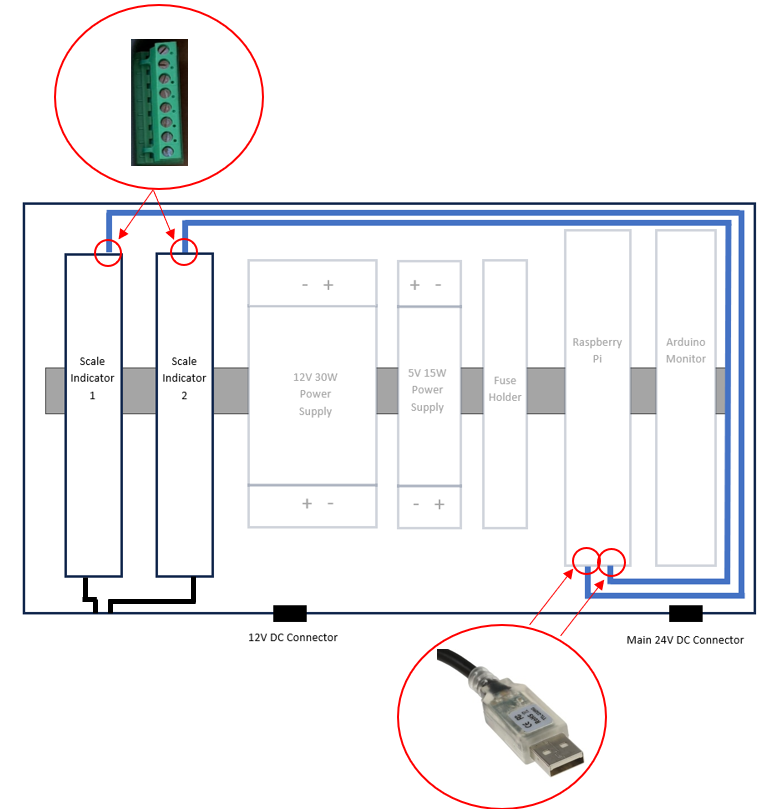
\includegraphics[width=7.29167in,height=\textheight,keepaspectratio]{images/media/41_connectors.png}

}

\caption{\textbf{Figure 41.1.} Laumas TLB485 scale indicator
connectors.}

\end{figure}%

\begin{itemize}
\item
  Only the orange and yellow wires of the RS485 converter is used. Strip
  and crimp ferrules on the end of the wires and connect as in Fig. 42.
\item
  Connect the GROUND and +12V power wires.
\end{itemize}

\begin{figure}[H]

{\centering 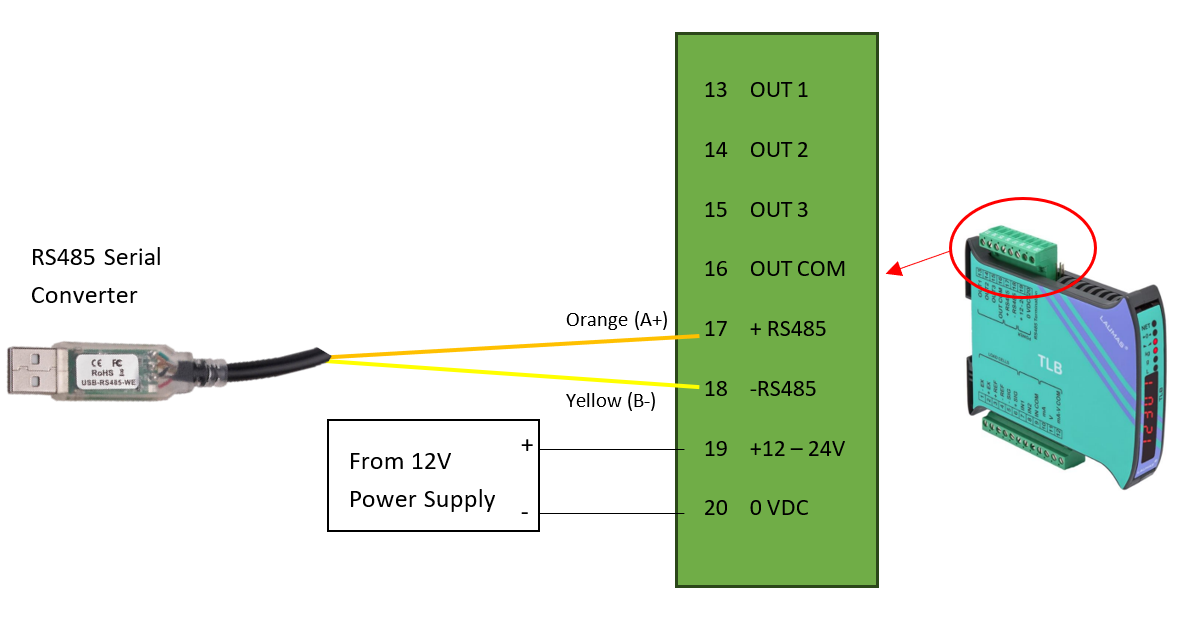
\includegraphics[width=4.16667in,height=\textheight,keepaspectratio]{images/media/42_usb_rs485.png}

}

\caption{\textbf{Figure 42.2.} Laumas TLB485 USB to RS485 wiring.}

\end{figure}%

\subsection{Indicator Scale
Connection}\label{indicator-scale-connection}

\begin{itemize}
\item
  Each scale connects to the APMS Main Unit via a 6-pin socket
  (111-5764), mounted on the front of the enclosure.
\item
  A short cable runs from the 6-pin socket to the x-pin connector for
  the GMT-X1 indicator, or if using a Laumas TLB485 the cable will run
  from the 6-pin socket connector to the 9-pin connector on the
  indicator (Fig. 43.2).
\end{itemize}

\begin{figure}[H]

{\centering 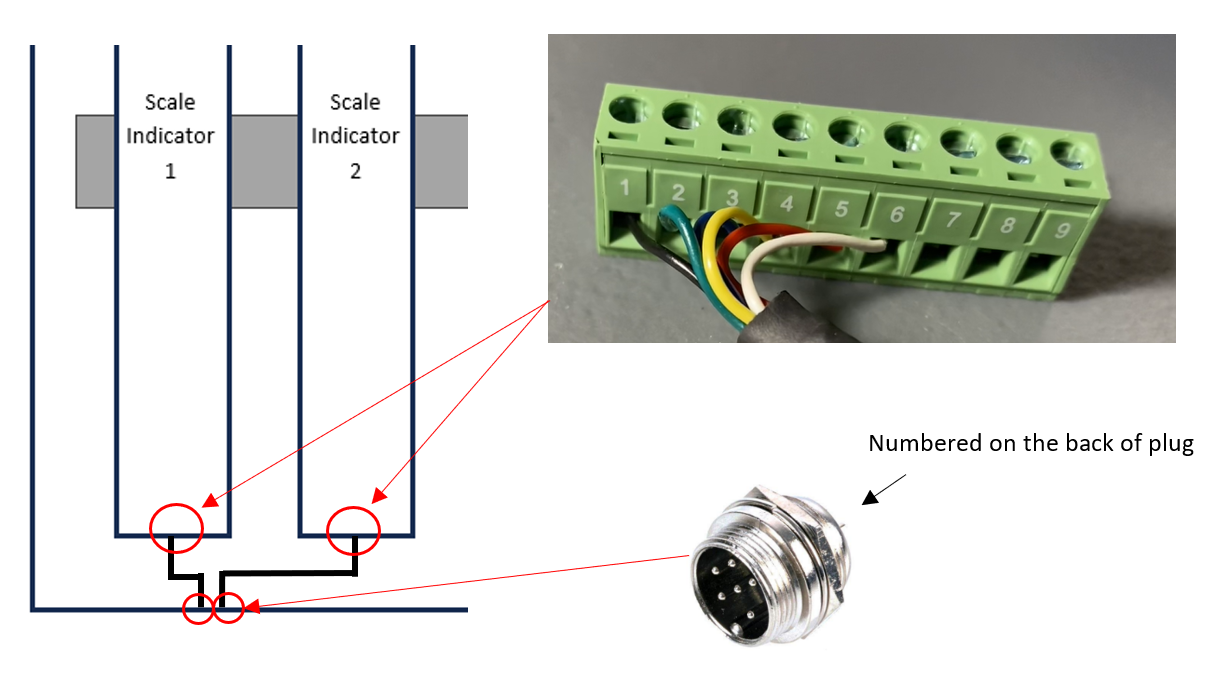
\includegraphics[width=4.16667in,height=\textheight,keepaspectratio]{images/media/43_loadcell_wiring.png}

}

\caption{\textbf{Figure 43.2.} Laumas TLB485 load cell wiring.}

\end{figure}%

\begin{itemize}
\item
  Each pin on the socket (111-5764) is numbered. Match the numbering on
  the 9-pin connector with that of the socket (only 1 - 6 is used). See
  Figs. 43 \& 44.
\item
  Solder the wires to the sockets and add ferrules before inserting it
  into the scale connector screw terminals.
\end{itemize}

\begin{figure}[H]

{\centering 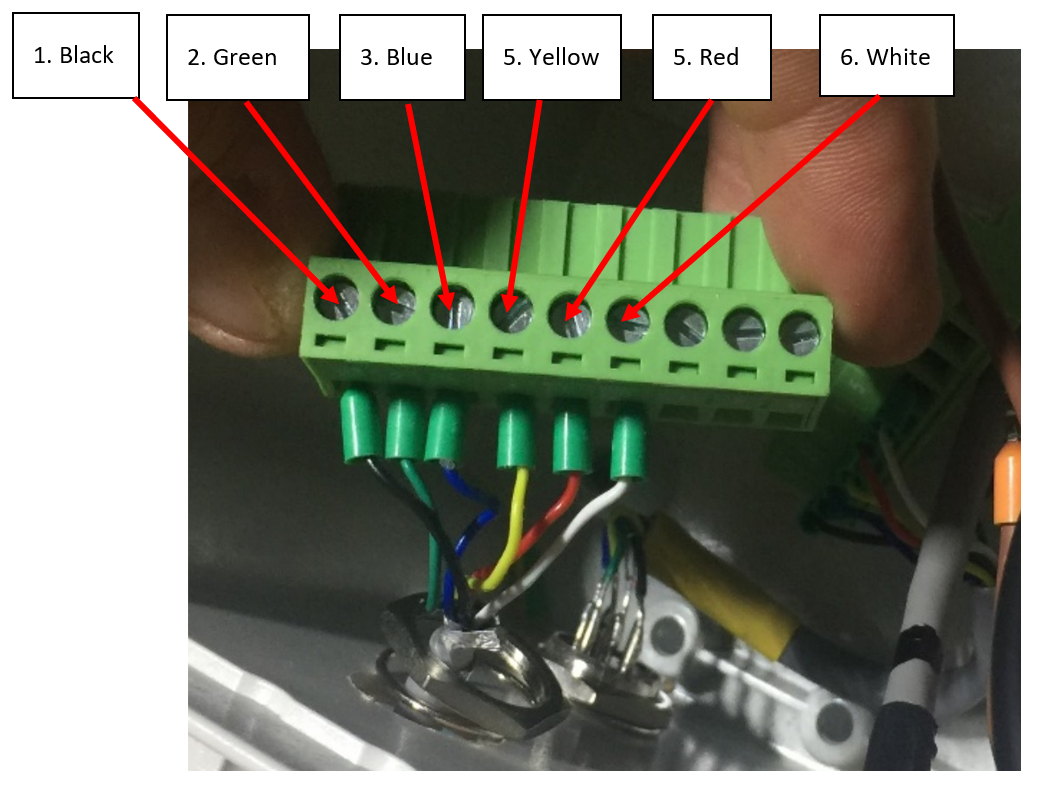
\includegraphics[width=4.16667in,height=\textheight,keepaspectratio]{images/media/44_6-pin_connector.png}

}

\caption{\textbf{Figure 44.} Installing 6-pin scale connector.}

\end{figure}%

\subsection{Jumper Install (Laumas TLB485
only)}\label{jumper-install-laumas-tlb485-only}

If using the Laumas TLB485 indicators, a jumper needs to be installed if
the baud-rate exceeds 9600. As we are communicating with the indicators
at a speed greater than 9600 BAUD, two jumpers need to be installed.
This is only applicable to TLB45 indicators and not the GMT-X1
indicators. Please see the excerpt from the manual below.

\begin{center}
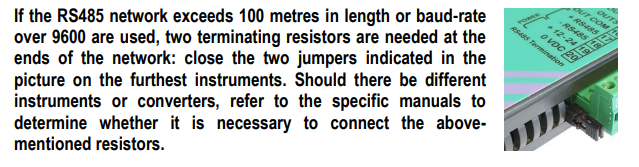
\includegraphics[width=6.25in,height=\textheight,keepaspectratio]{images/media/44_tlb_manual.png}
\end{center}

\subsection{Configuring The Scale
Indicators}\label{configuring-the-scale-indicators}

\begin{itemize}
\item
  Before configuring the scale indicators, check that it has been wired
  correctly and working properly:

  \begin{itemize}
  \item
    Plug in both the 6- and 9-pin scale connectors.
  \item
    Plug the scales into their respective scale sockets
  \item
    Apply power to the Main Unit -- the indicators should light up and
    show a weight after start-up.
  \item
    Apply light pressure on Scale 1 and Scale 2 and confirm the correct
    indicator changes its weight reading.
  \end{itemize}
\end{itemize}

To configure the scale indicators, the front cover is flipped open and
the buttons on the device are used. There are four buttons on each
indicator as in Fig. 46.

\begin{figure}[H]

{\centering 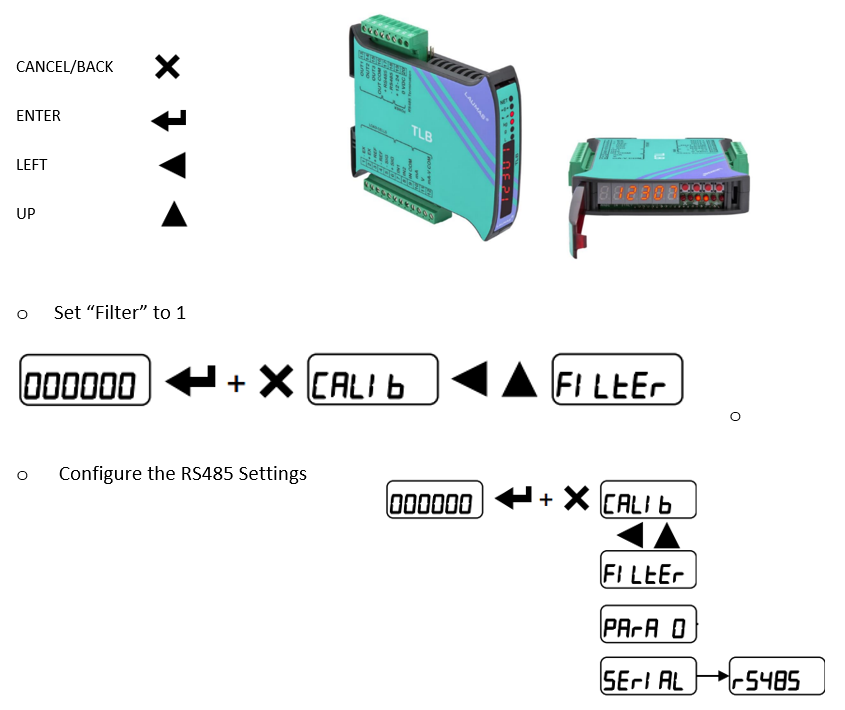
\includegraphics[width=6.25in,height=\textheight,keepaspectratio]{images/media/45_rs485.png}

}

\caption{\textbf{Figure 46.}}

\end{figure}%

\begin{longtable}[]{@{}
  >{\raggedright\arraybackslash}p{(\linewidth - 2\tabcolsep) * \real{0.3229}}
  >{\raggedright\arraybackslash}p{(\linewidth - 2\tabcolsep) * \real{0.6562}}@{}}
\toprule\noalign{}
\begin{minipage}[b]{\linewidth}\raggedright
\textbf{Name}
\end{minipage} & \begin{minipage}[b]{\linewidth}\raggedright
\textbf{Value}
\end{minipage} \\
\midrule\noalign{}
\endhead
\bottomrule\noalign{}
\endlastfoot
Mode & Continuous \\
BAUD rate & 115200 \\
Hertz & 100 \\
Parity & None \\
Stop Bit & 1 \\
Mode & \emph{nodt} \\
\end{longtable}

The settings above will be checked when testing the scales script (See:
\hyperref[Testingux5cux2520theux5cux2520scales.pyux5cux2520script]{Testing
the scales.py Script})

\section{Installing the APMS Monitor}\label{installing-the-apms-monitor}

If the APMS Monitor has been tested as explained in
\hyperref[Testingux5cux2520theux5cux2520Monitorux5cux2520Circuitux5cux2520Board]{Testing
the Monitor Circuit Board}, it can be installed in the APMS Main Unit.
The Monitor is mounted on a 3D printed mounting plate, as discussed
earlier.

\begin{itemize}
\item
  The Monitor mounting plate clips on to the DIN rail, with the power
  connector facing the front of the Main Unit, and the 12V monitoring
  connector facing towards the back (Fig. 47).
\item
  Connect the power and 12V monitoring wires.
\item
  Connect the 40-pin Raspberry Pi ribbon cable.
\end{itemize}

\begin{figure}[H]

{\centering 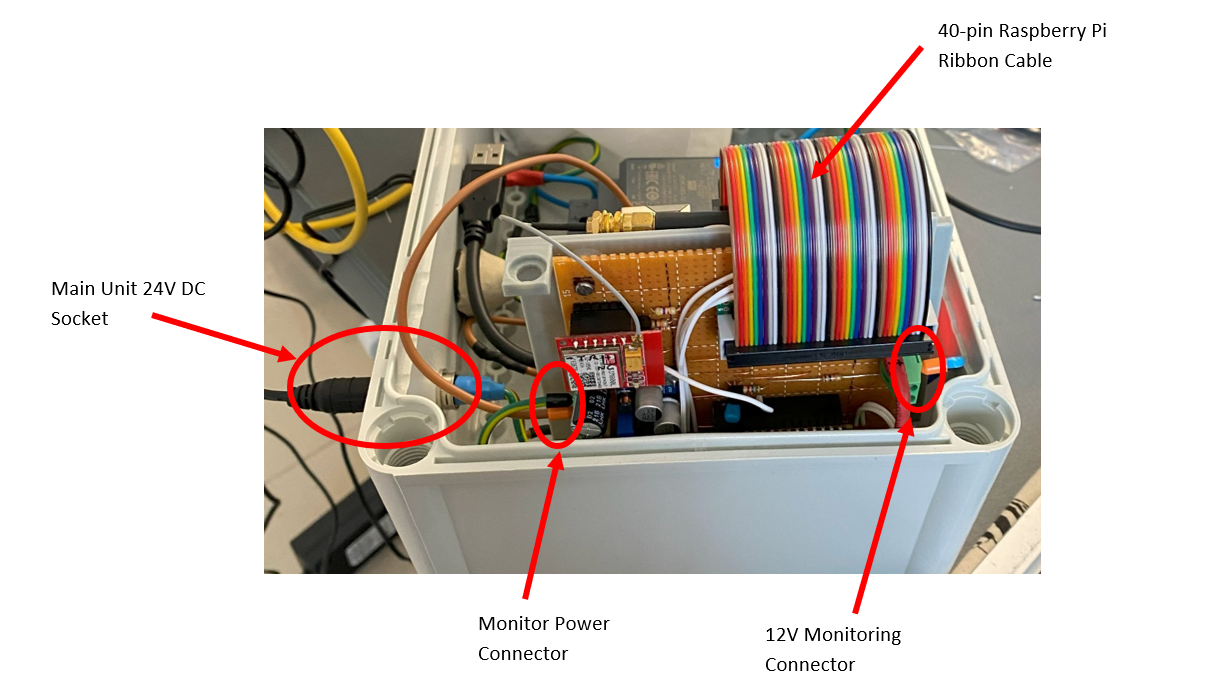
\includegraphics[width=4.16667in,height=\textheight,keepaspectratio]{images/media/46_monitor.png}

}

\caption{\textbf{Figure 47.} Monitor board mounted inside the APMS Main
Unit.}

\end{figure}%

\part{Software \& Configuration}

\chapter{AWS S3 Cloud Storage}\label{aws-s3-cloud-storage}

The software and data are stored on the AWS S3 Server.

\section{Administrator Details}\label{administrator-details}

To access the software, download a S3 Client, such as S3 Browser.
(\url{https://s3browser.com/}).

The usernames, passwords and other confidential information is stored in
a separate document.

There are currently five main objects:

\begin{longtable}[]{@{}
  >{\centering\arraybackslash}p{(\linewidth - 2\tabcolsep) * \real{0.4316}}
  >{\raggedright\arraybackslash}p{(\linewidth - 2\tabcolsep) * \real{0.5579}}@{}}
\toprule\noalign{}
\begin{minipage}[b]{\linewidth}\centering
\textbf{Directory}
\end{minipage} & \begin{minipage}[b]{\linewidth}\raggedright
\textbf{Description of contents}
\end{minipage} \\
\midrule\noalign{}
\endhead
\bottomrule\noalign{}
\endlastfoot
3://apmsbirdlife/APMS/data/ & This holds all the scale, rfid and system
status data. \\
3://apmsbirdlife/APMS/software/ & This holds all the necessary software
to set up a new system. \\
3://apmsbirdlife/APMS/documents/ & This holds documentation such as the
manual, parts lists etc. \\
3://apmsbirdlife/APMS/3D\_prints/ & This holds the design files for the
various 3D printed parts \\
3://apmsbirdlife/APMS/website/ & This holds the daily plots for the
website run by Ninepoint \\
\end{longtable}

\begin{tcolorbox}[enhanced jigsaw, left=2mm, toptitle=1mm, breakable, opacitybacktitle=0.6, title=\textcolor{quarto-callout-note-color}{\faInfo}\hspace{0.5em}{Note}, colback=white, opacityback=0, rightrule=.15mm, leftrule=.75mm, colbacktitle=quarto-callout-note-color!10!white, bottomtitle=1mm, titlerule=0mm, coltitle=black, colframe=quarto-callout-note-color-frame, arc=.35mm, bottomrule=.15mm, toprule=.15mm]

The firmware running on the Raspberry Pi and the code for the Dashboard
can all be found on the \href{https://www.github.com/apmsbirdlife}{APMS
BirdLife GithUB} repository.

\end{tcolorbox}

\section{Creating a User on AWS S3}\label{creating-a-user-on-aws-s3}

Each Raspberry Pi has an AWS S3 Username, Access Key and Secret Access
Key assigned to it. This enables the data and log files to be uploaded
to the cloud every day. When installing an APMS at a new site, a new
user for the site must be created. This manual is accurate as of writing
in December 2023, but as websites and services change, slight variations
might appear in future. Please update this manual when deemed necessary
and update the revision number. Further improvement regarding security,
such as using IAM Identity Center instead of IAM, using Multi Factor
Authentication or using AWS CLI2, are left up to the discretion of the
administrator

\begin{itemize}
\item
  Go to \url{https://aws.amazon.com/s3/}
\item
  Click on ``\emph{Sign in to console}'' in the top right.
\end{itemize}

\begin{center}
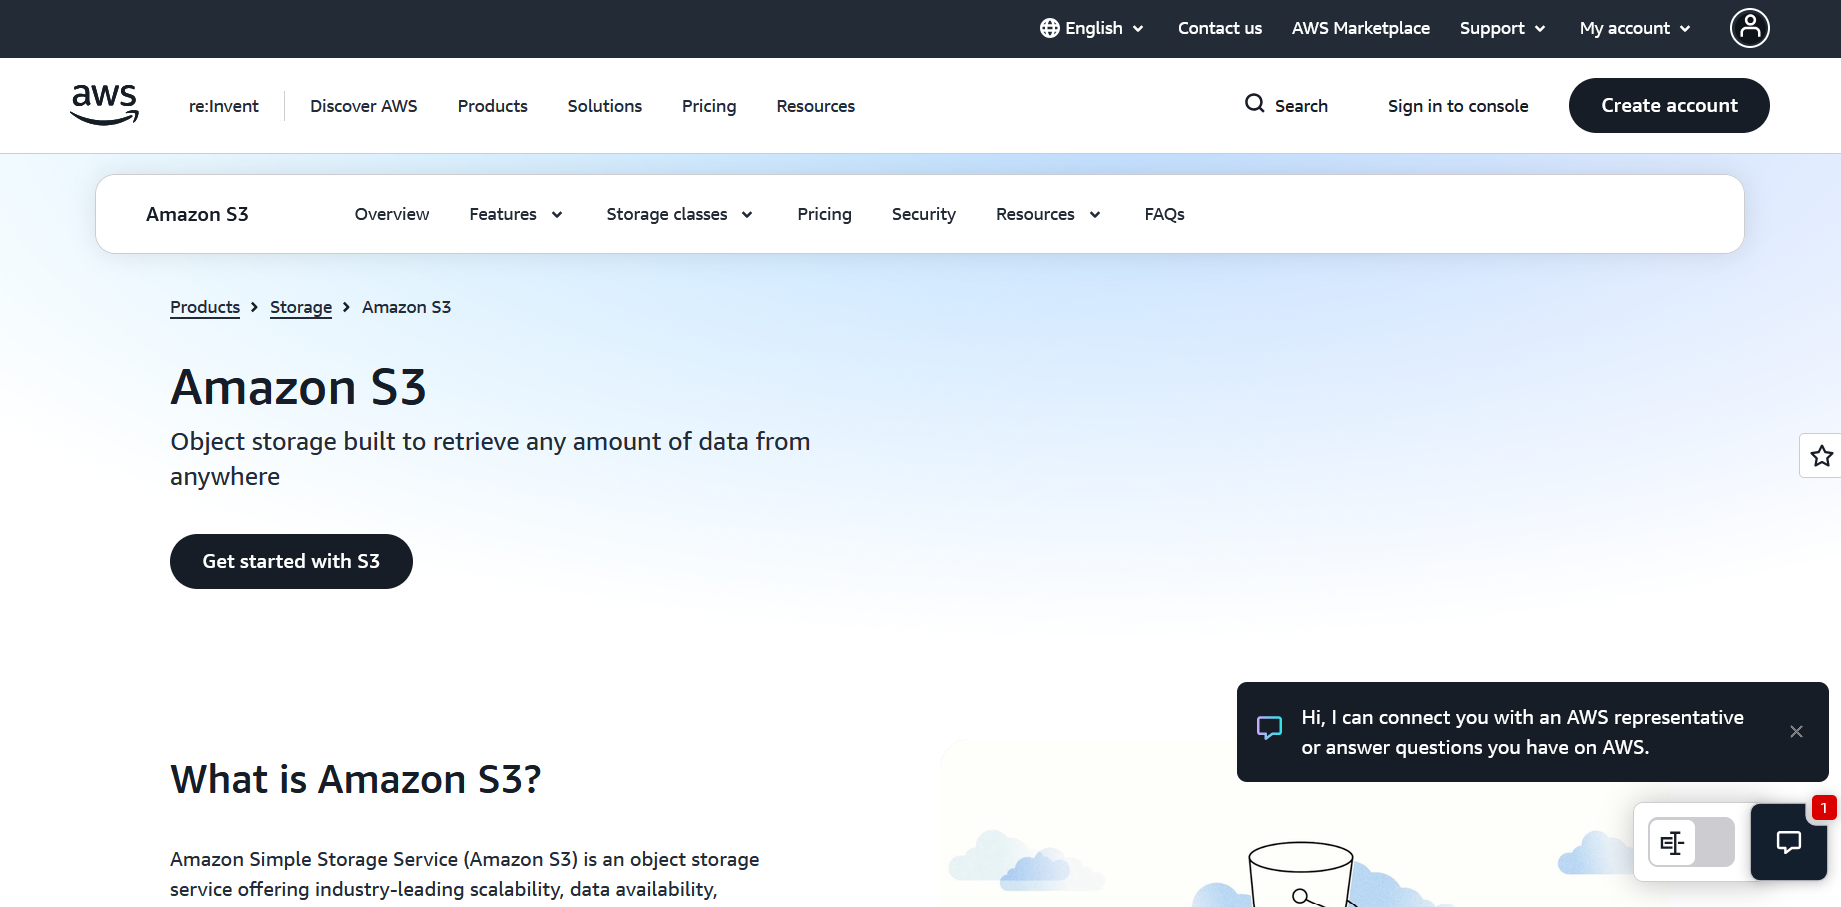
\includegraphics[width=6.25in,height=\textheight,keepaspectratio]{images/media/48_1_aws.png}
\end{center}

\begin{itemize}
\tightlist
\item
  Click ``\emph{Sign in using root user's email}''.
\end{itemize}

\begin{center}
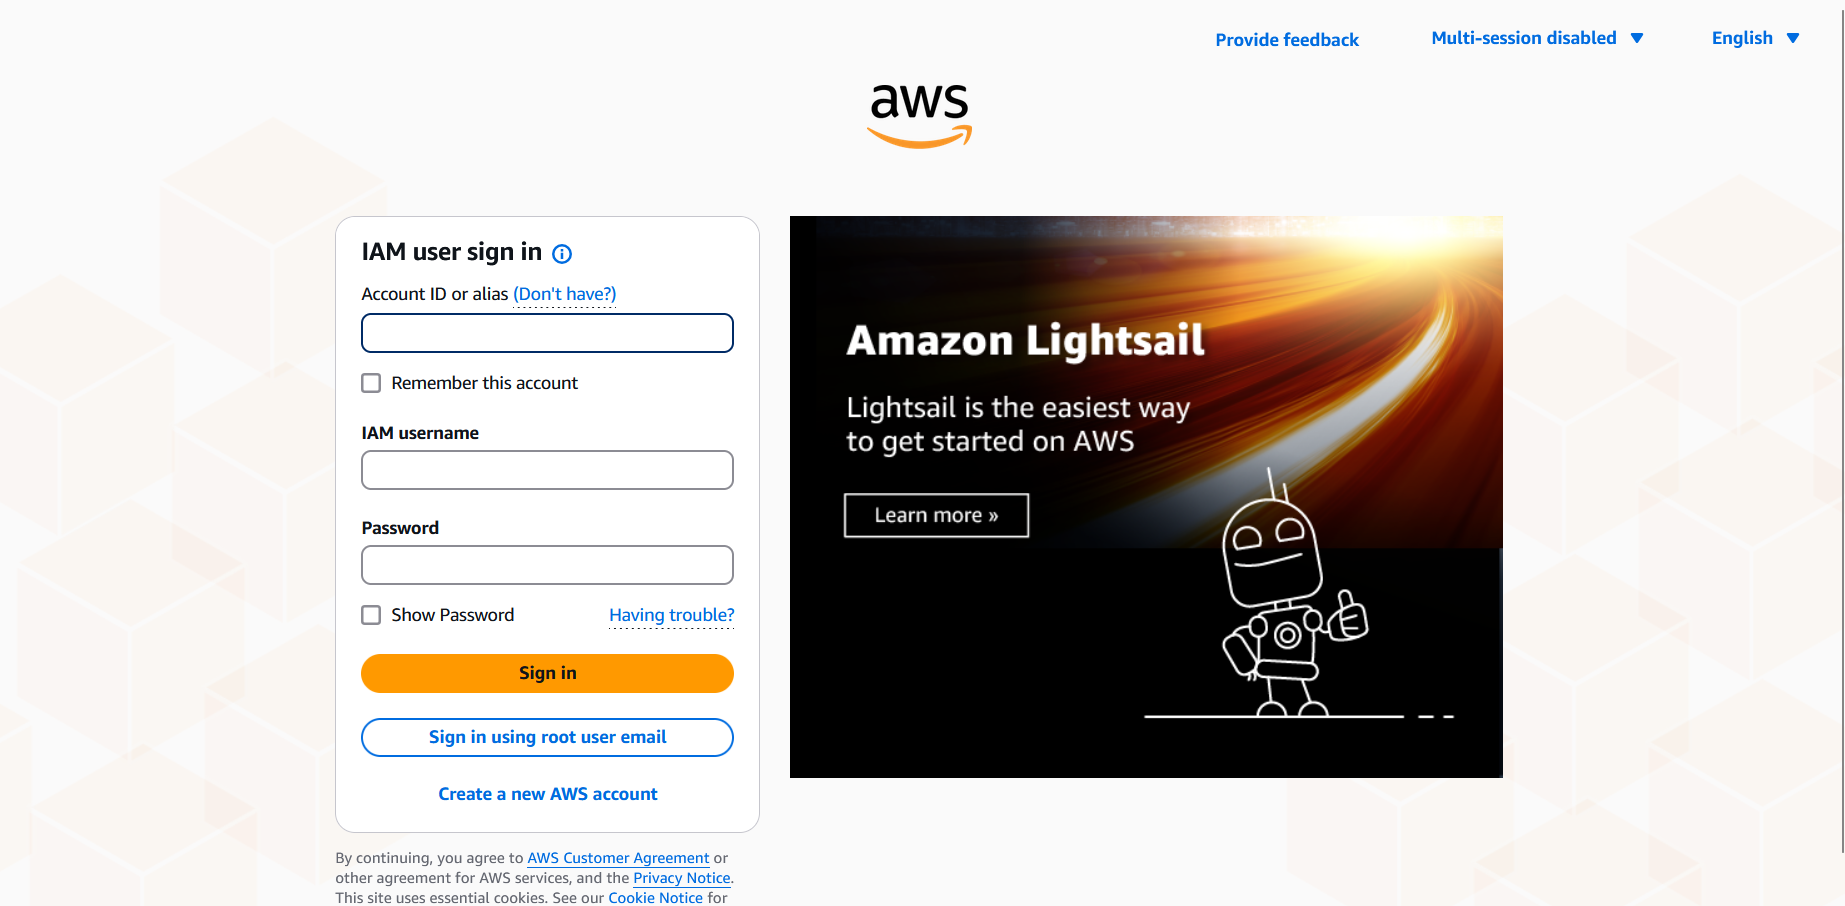
\includegraphics[width=6.25in,height=\textheight,keepaspectratio]{images/media/48_2_aws.png}
\end{center}

\begin{itemize}
\tightlist
\item
  Log using the relevant account details.
\end{itemize}

\begin{center}

\includegraphics[width=6.25in,height=\textheight,keepaspectratio]{images/media/48_3_aws.png}
\end{center}

\begin{itemize}
\tightlist
\item
  Click on ``\emph{IAM}'' (NOT ``IAM Identity Center'').
\end{itemize}

\begin{center}
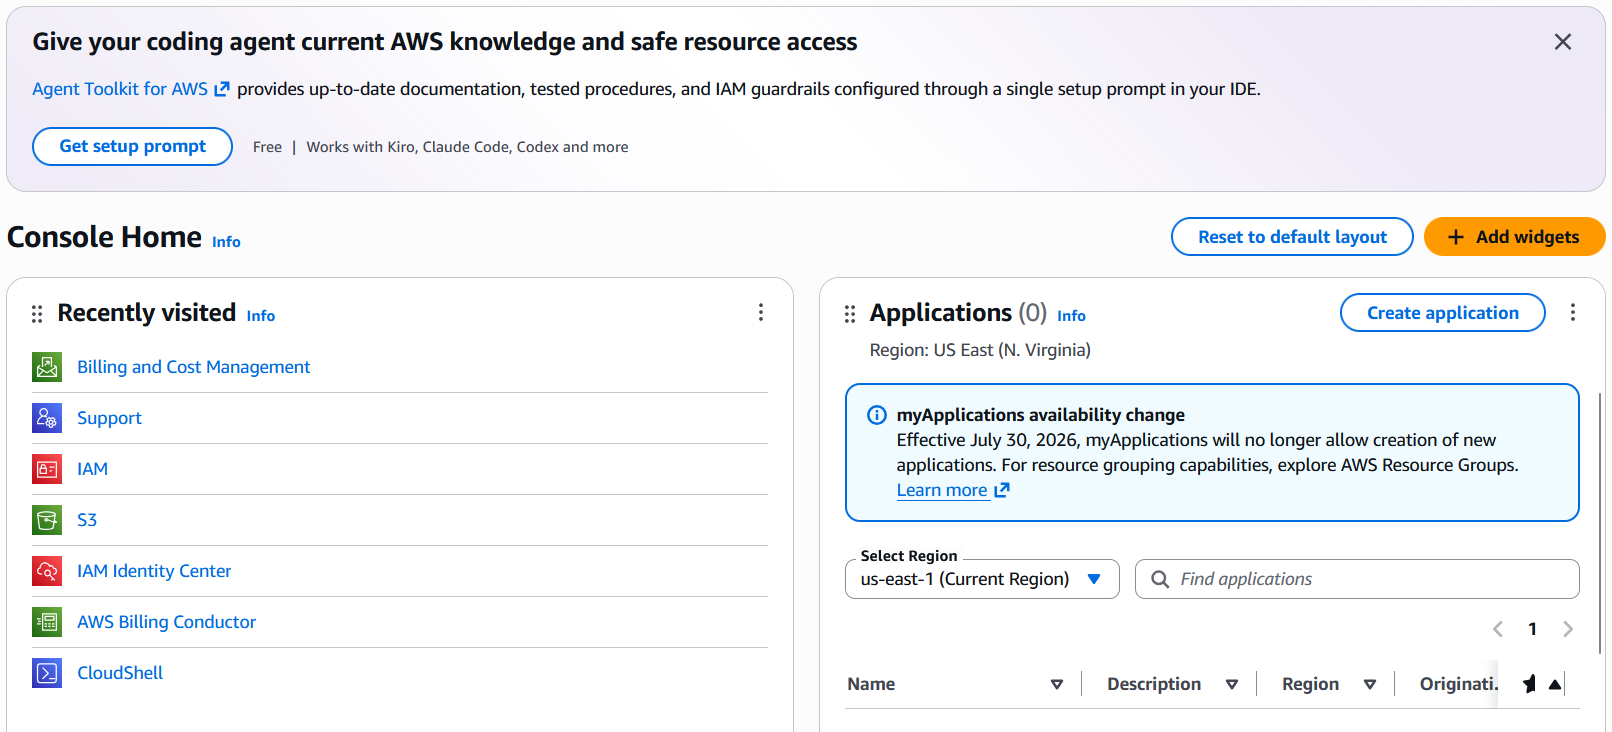
\includegraphics[width=6.25in,height=\textheight,keepaspectratio]{images/media/48_4_aws.png}
\end{center}

\begin{itemize}
\tightlist
\item
  Click on ``\emph{IAM Users}'' and then in the top right,
  ``\emph{Create User}''.
\end{itemize}

\begin{center}
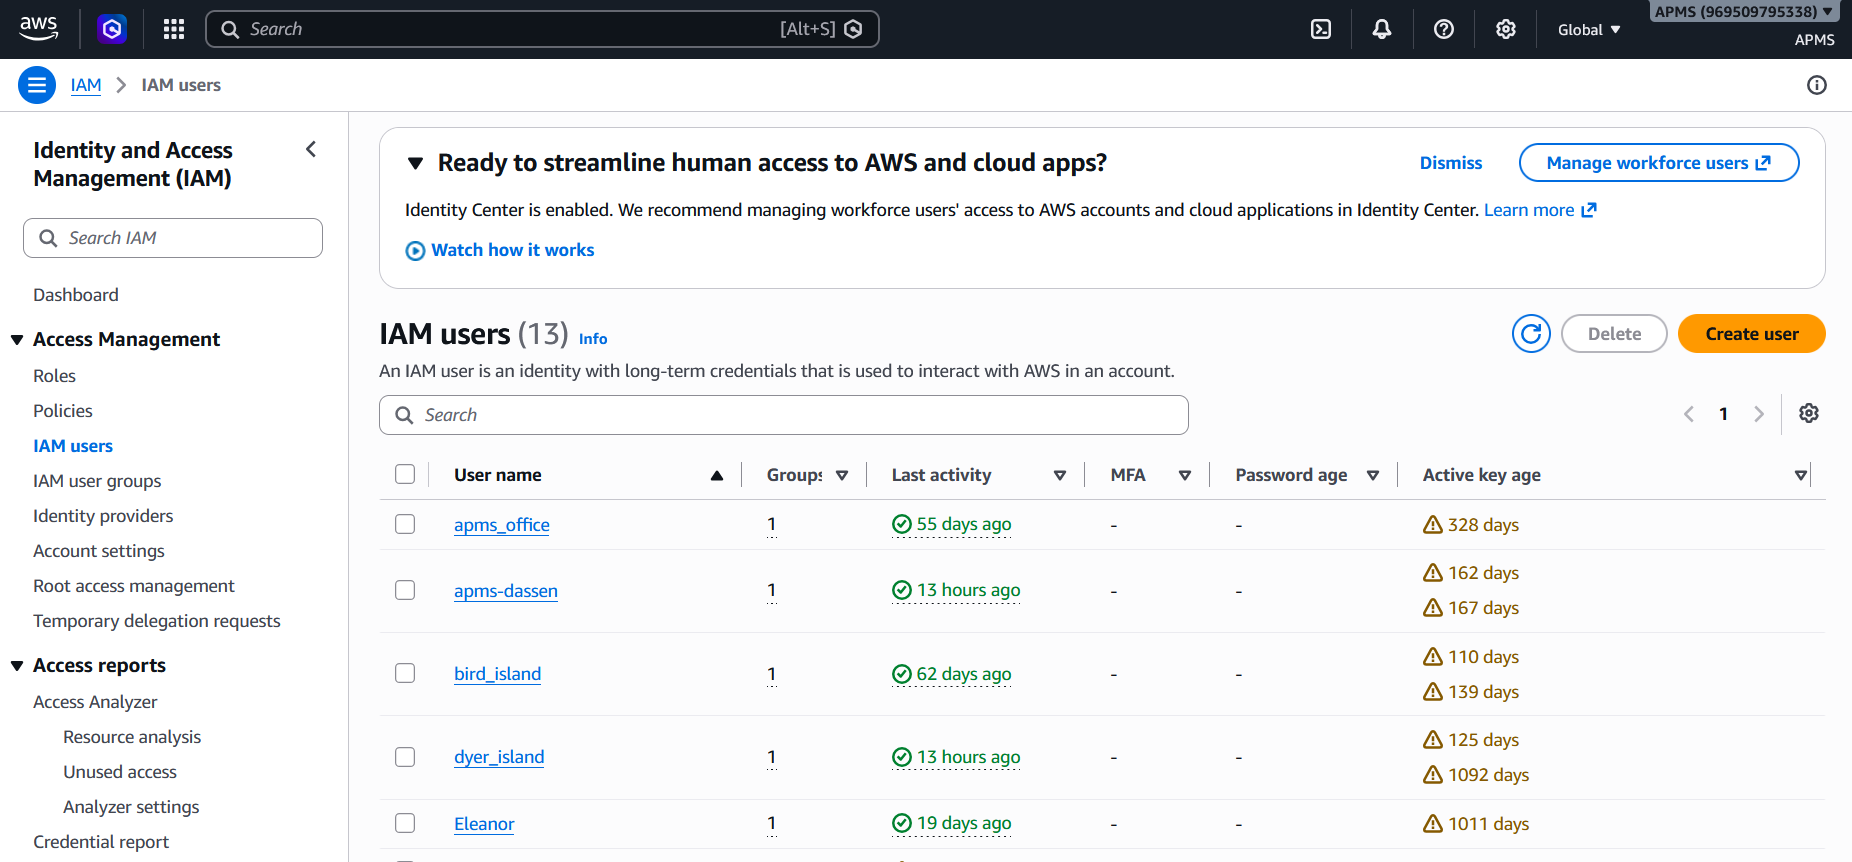
\includegraphics[width=6.25in,height=\textheight,keepaspectratio]{images/media/48_5_aws.png}
\end{center}

\begin{itemize}
\tightlist
\item
  Under ``\emph{User name}'', enter the site name, all lower case
  letters. Example: ``apms\_boulders''. Keep all the defaults as is.
  Click Next to continue.
\end{itemize}

\begin{center}
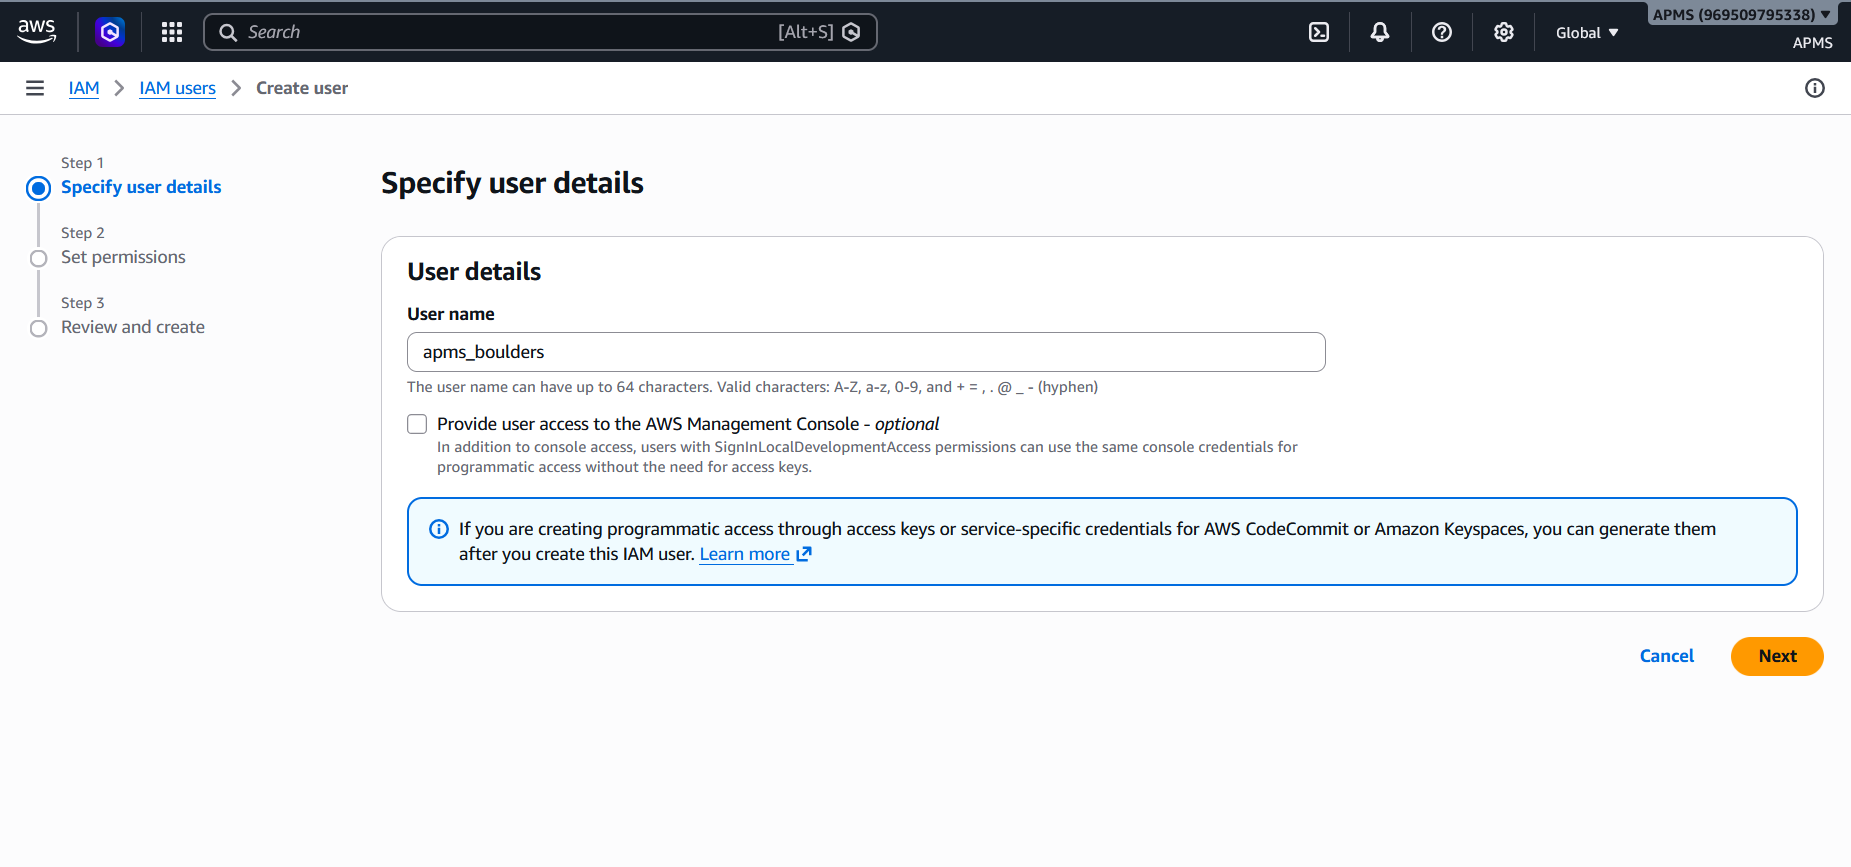
\includegraphics[width=6.25in,height=\textheight,keepaspectratio]{images/media/48_6_aws.png}
\end{center}

\begin{itemize}
\tightlist
\item
  On the ``\emph{Set permissions}'' page, select the S3\_Full\_Access
  option under user groups and click ``\emph{Next}''.
\end{itemize}

\begin{center}
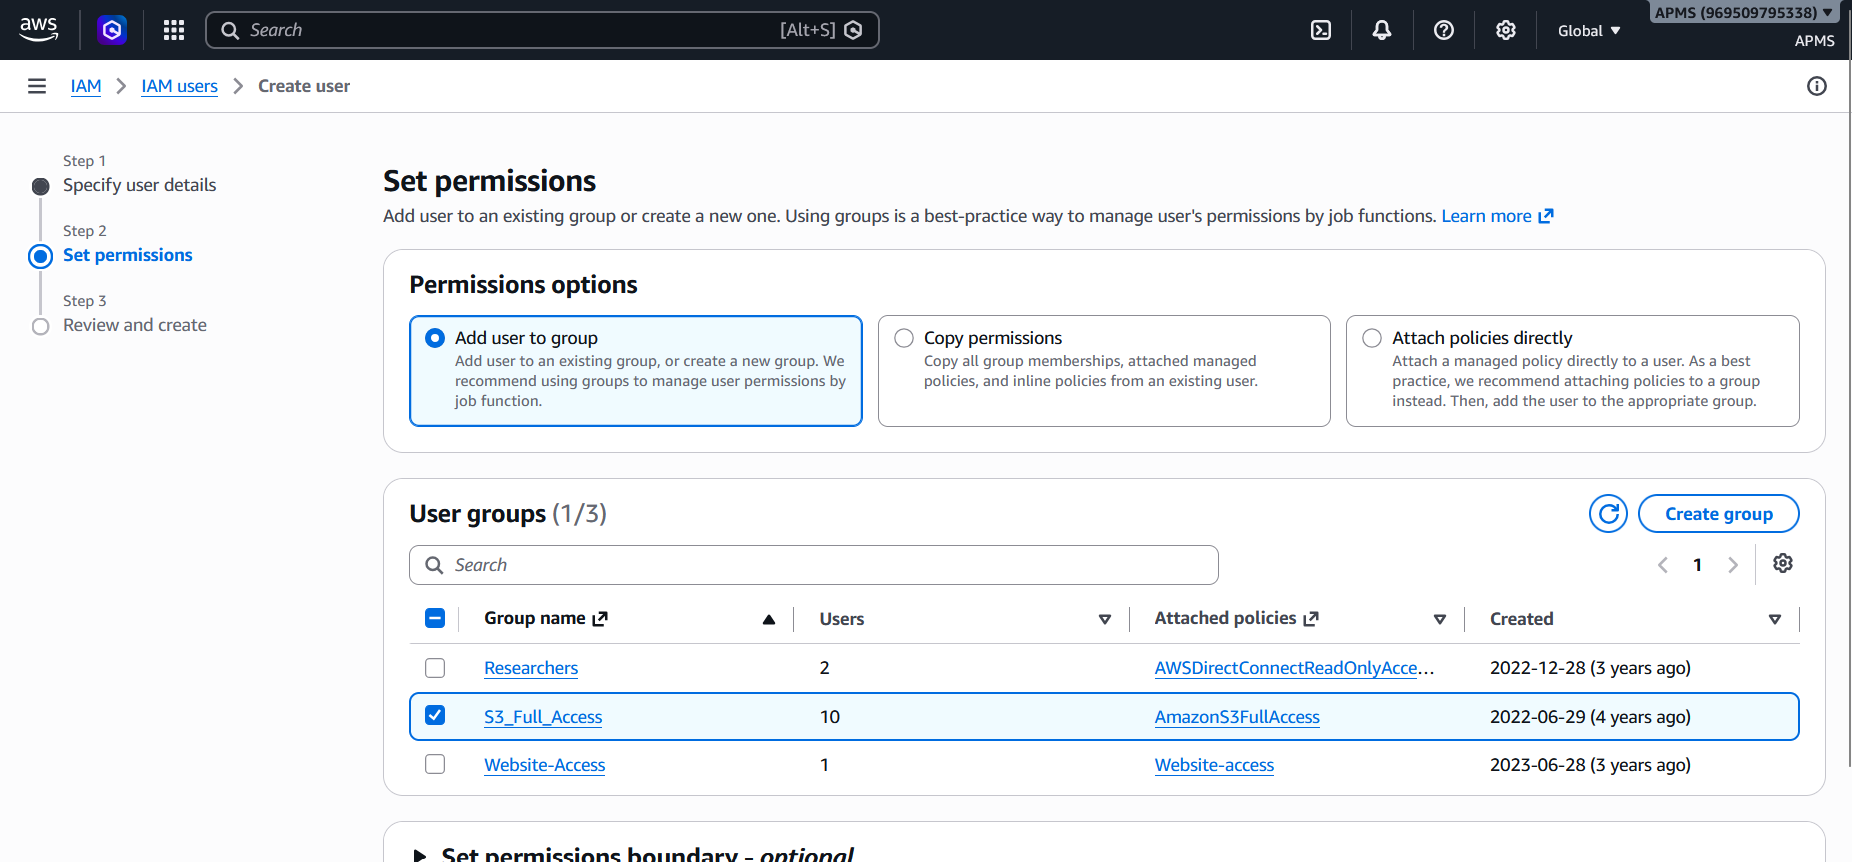
\includegraphics[width=6.25in,height=\textheight,keepaspectratio]{images/media/48_7_aws.png}
\end{center}

\begin{itemize}
\item
  On the ``\emph{Review and create}'' page, click on ``\emph{Create
  user}''.
\item
  Now view the new user that you created and navigate to
  ``\emph{Security credentials}'' and then scroll down to ``\emph{Access
  keys}''
\end{itemize}

\begin{center}
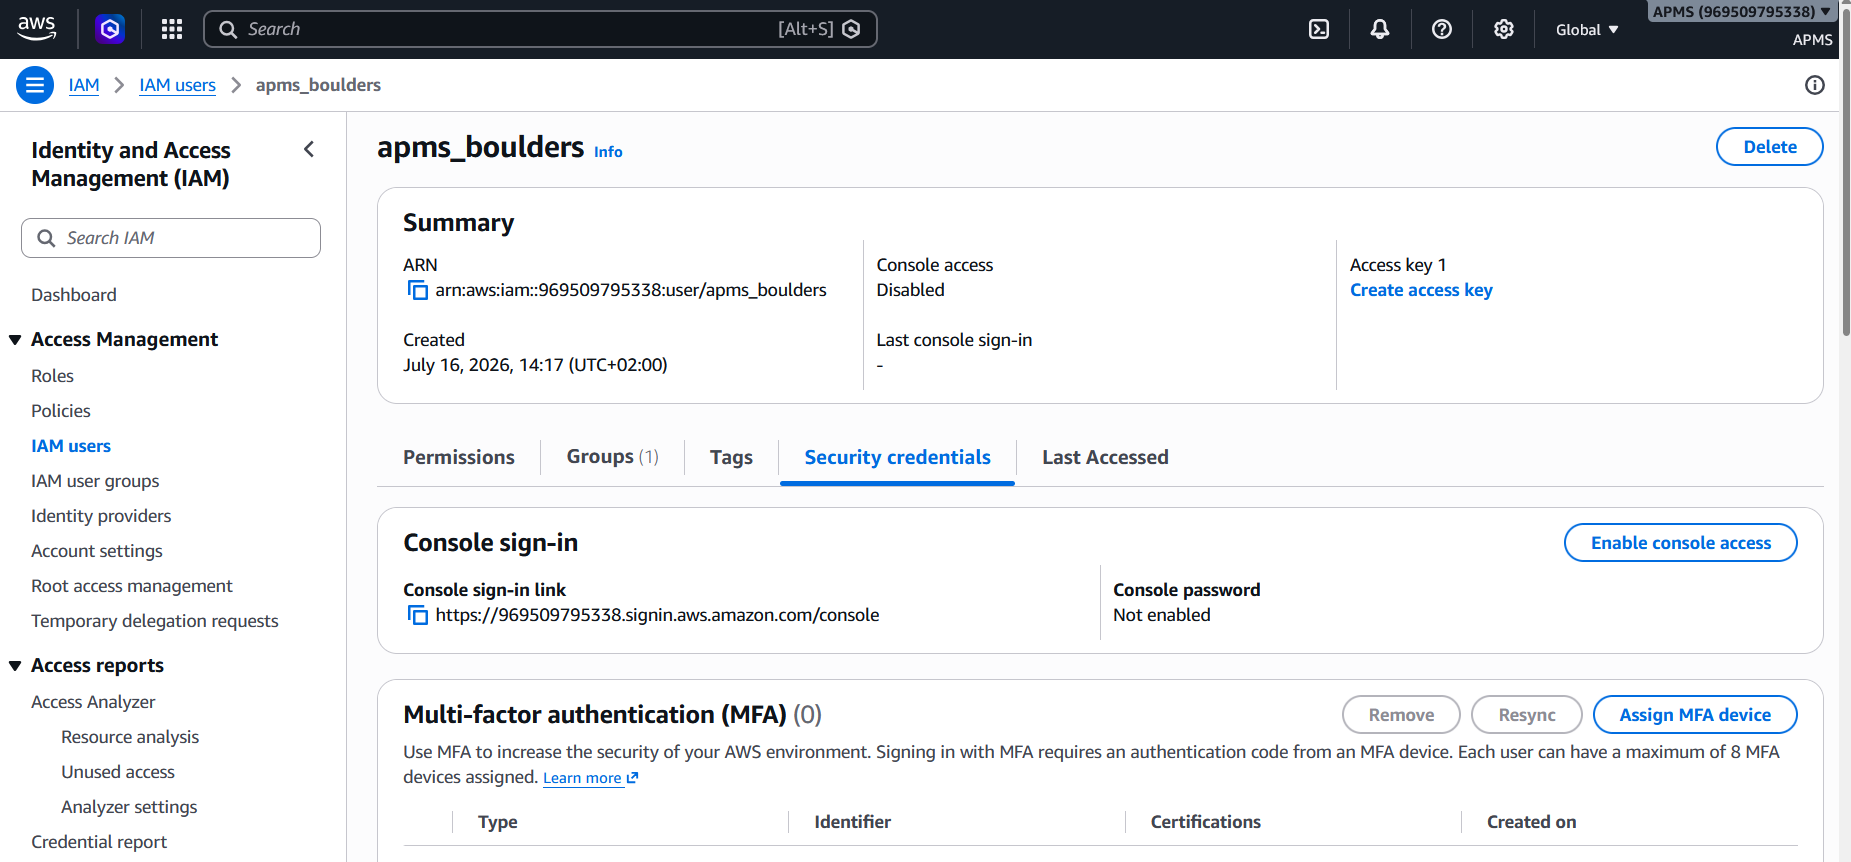
\includegraphics[width=6.25in,height=\textheight,keepaspectratio]{images/media/48_8_aws.png}
\end{center}

\begin{itemize}
\item
  Click on ``\emph{Create access key}''
\item
  Click on ``\emph{Command Line Interface (CLI)}'', click the
  ``\emph{Confirmation}'' and click ``\emph{Next}''
\end{itemize}

\begin{center}
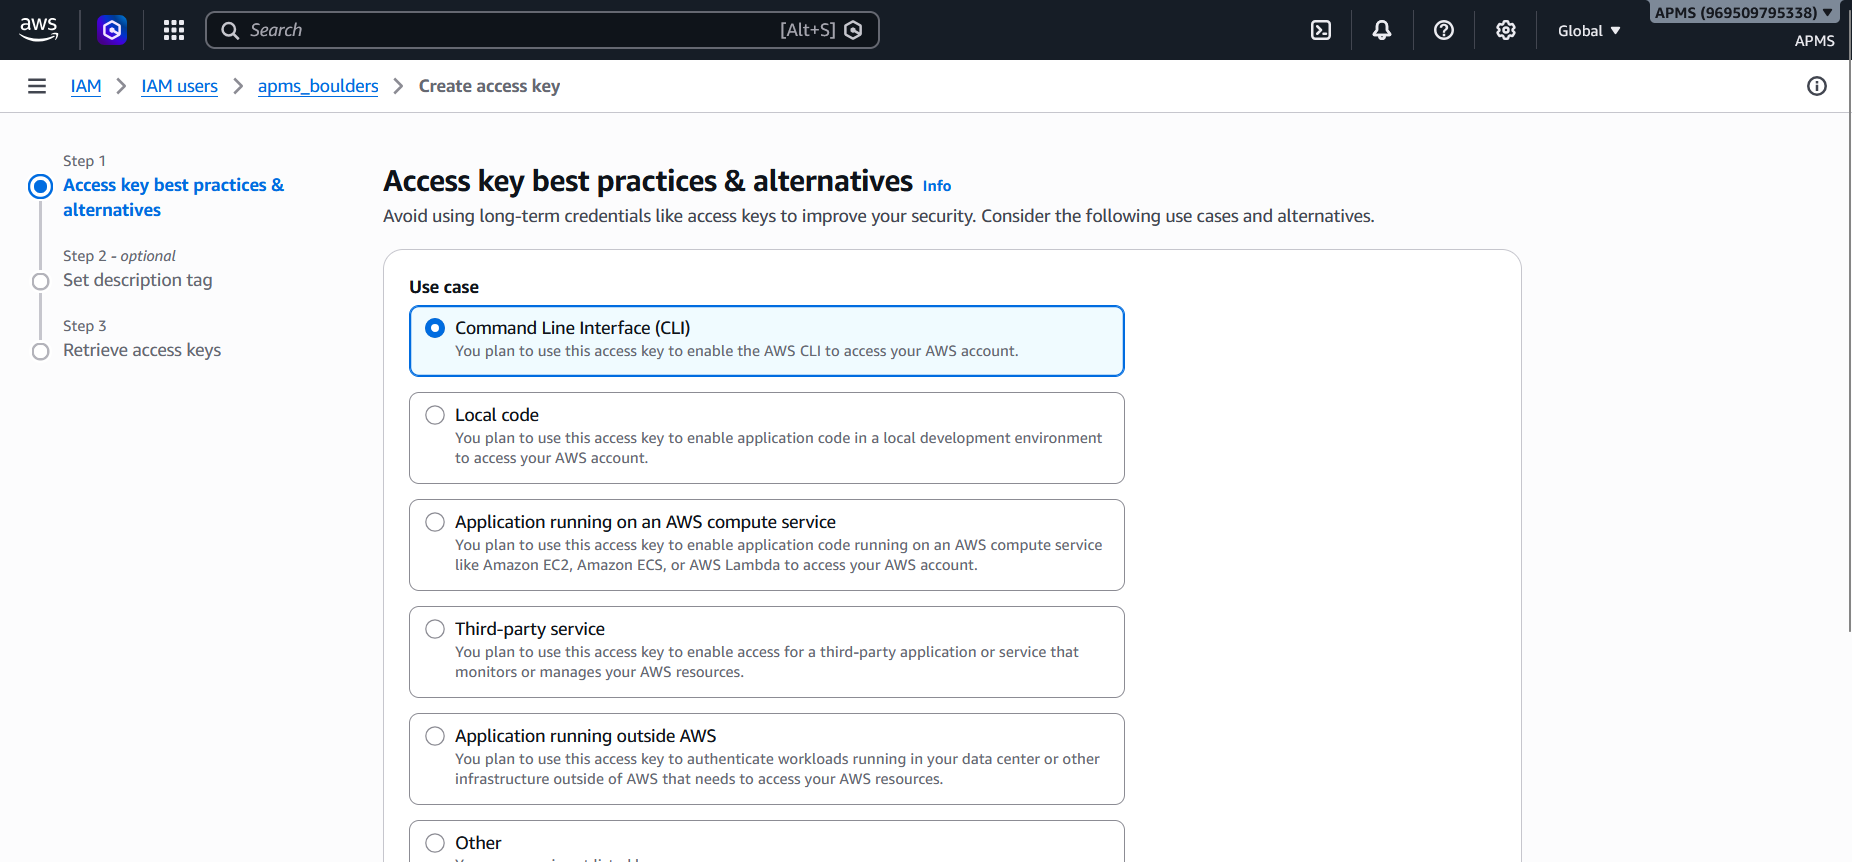
\includegraphics[width=6.25in,height=\textheight,keepaspectratio]{images/media/48_9_aws.png}
\end{center}

\begin{itemize}
\tightlist
\item
  On the ``\emph{Set description tag}'' page, enter ``\emph{APMS
  upload}'' and click on ``\emph{Create access key}''
\end{itemize}

\begin{center}
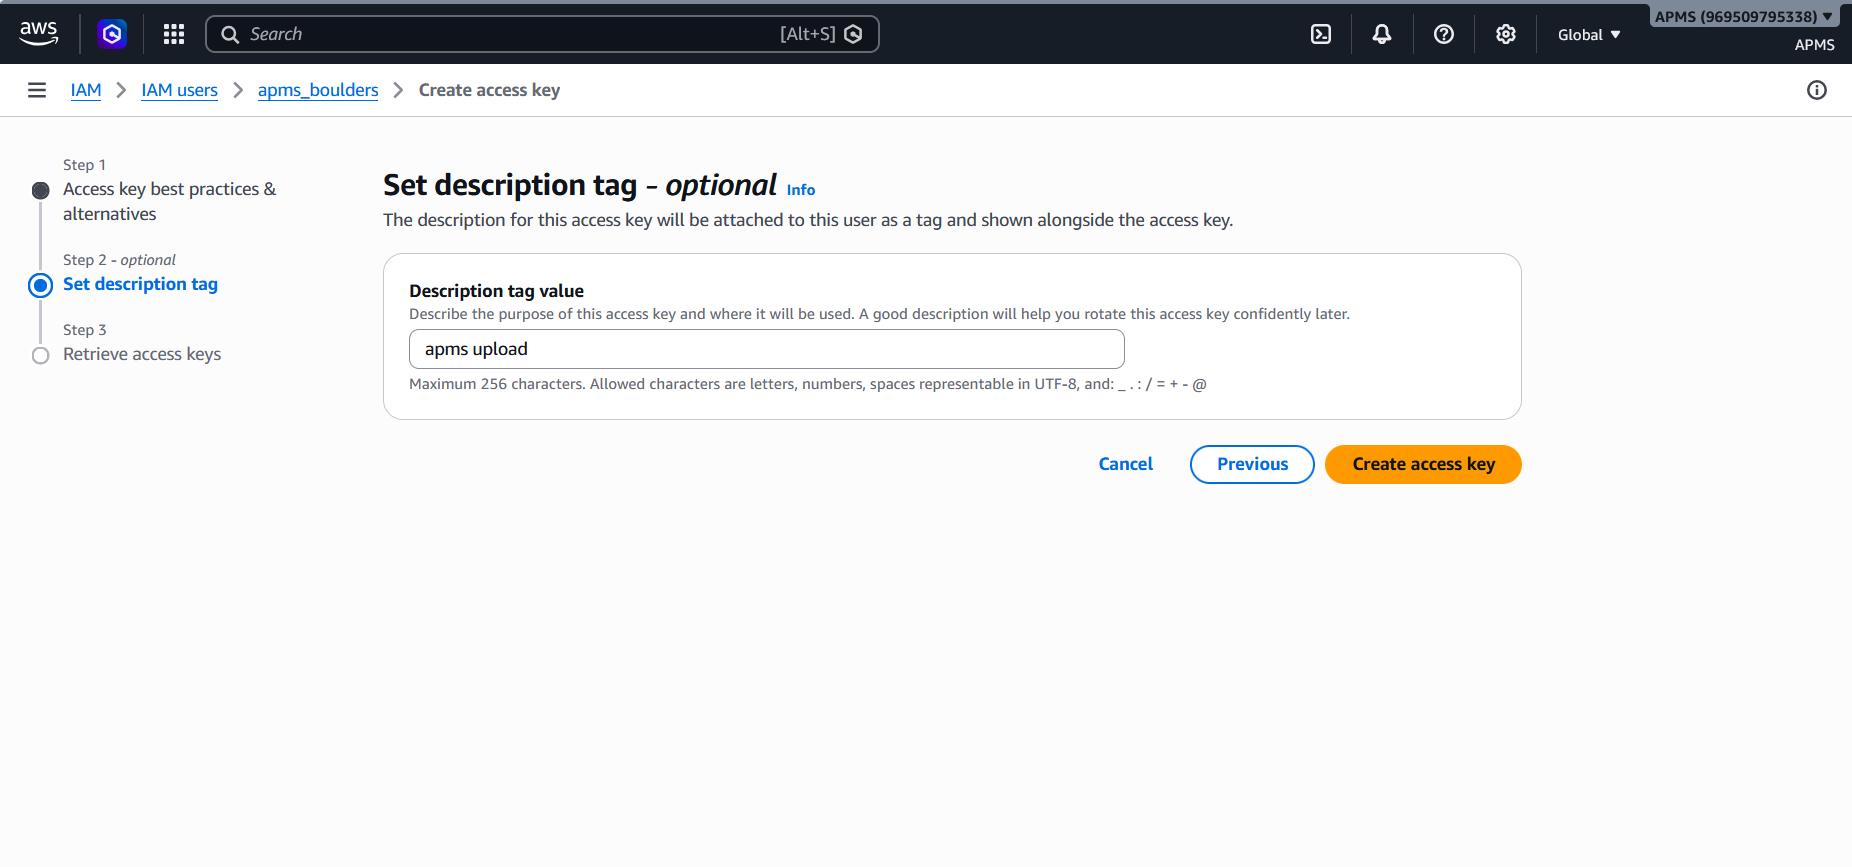
\includegraphics[width=6.25in,height=\textheight,keepaspectratio]{images/media/48_10_aws.png}
\end{center}

\begin{itemize}
\tightlist
\item
  You have now successfully created a user for the new site and created
  an access key. Copy down the Access key and Secret access key (Click
  ``\emph{Show}''). You can also download the .csv file containing this
  information. Please keep this information very secure as it has full
  read/write access to the cloud. Also, please note that you will not be
  able to view this information at a later stage, so make sure it is
  stored safely. If this information is lost, and is needed in future,
  create a new user as described in this section.
\end{itemize}

\begin{center}
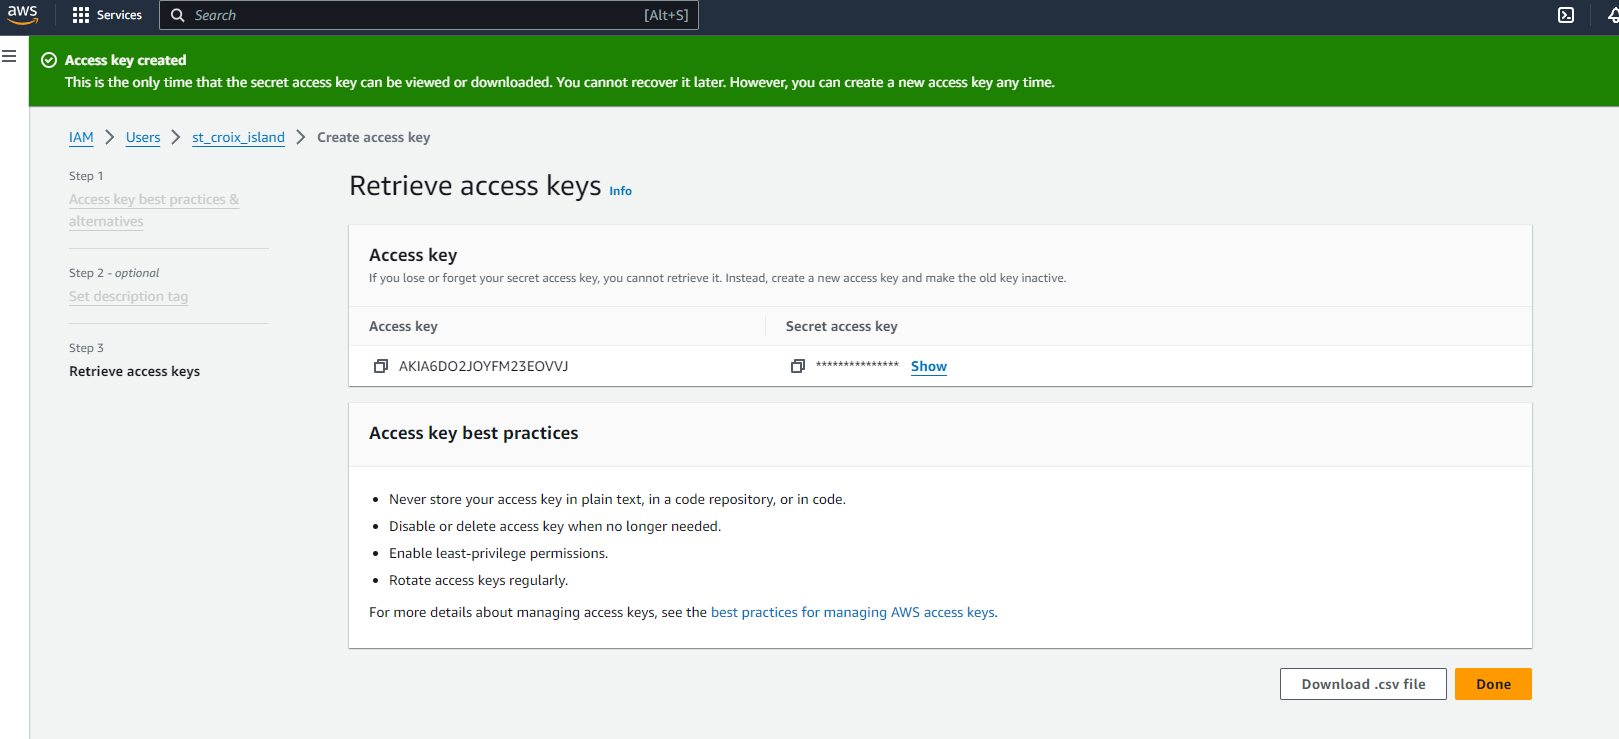
\includegraphics[width=6.25in,height=\textheight,keepaspectratio]{images/media/image103.png}
\end{center}

This access key and secret access key will be needed when the APMS is
configured. See
\hyperref[Configuringux5cux2520theux5cux2520APMS]{Configuring the APMS}.

\chapter{Raspberry Pi Operating
System}\label{raspberry-pi-operating-system}

The Raspberry Pi operating system must be installed first, together with
all required libraries and applications. A microSD card, SD card reader
and a computer running Windows is needed for this step. If the operating
system is being installed on a spare Raspberry Pi, a USB-C cable and 5V
3A power supply will be needed to power the device.

\section{Prepare the micro SD card}\label{prepare-the-micro-sd-card}

\begin{itemize}
\item
  Get a new SD card (currently using a 64GB SanDisk) and insert it into
  the MicroSD card reader.
\item
  Download the Rpi Imager and Rpi OS from the cloud
  (APMS/software/RaspberryPi)

  \begin{itemize}
  \tightlist
  \item
    The Imager can also be downloaded online here:
    \href{https://github.com/raspberrypi/rpi-imager/releases?page=3\#release-v1.7.4}{Download
    RPi Imager v1.7.4}.
  \item
    One way to do this is to download S3 Browser and navigate to the
    relevant software folder
    (\href{https://s3browser.com/}{\ul{https://s3browser.com/}} )
  \item
    If you don't have access to the AWS S3 cloud, you can also download
    it from here:
    \href{https://os.watch/raspberrypios/2023-02-21}{Download Pi OS
    bullseye}. Make sure it's the
    ``2023-02-21-raspios-bullseye-arm64-lite.img'' version.
  \end{itemize}
\item
  Install and run Raspberry Pi Imager (Version 1.7.4 for Windows used
  for this manual)

  \begin{itemize}
  \tightlist
  \item
    Choose OS\\
  \item
    Select ``Use custom''
  \item
    Select the raspberry pi image you downloaded
  \item
    All our APMSs are running on \emph{Raspi OS Bullseye 2023-02-21}
    ``2023-02-21-raspios-bullseye-arm64-lite.img''
  \end{itemize}
\item
  CHOOSE STORAGE and select the SD card.
\item
  Click on the settings cog.

  \begin{itemize}
  \item
    Choose a hostname. Example: ``apms-dyer'' or ``apms-boulders''
  \item
    Select ``Enable SSH''

    \begin{itemize}
    \tightlist
    \item
      ``Use password authentication''
    \end{itemize}
  \item
    Select ``Set username and password''

    \begin{itemize}
    \tightlist
    \item
      username: apms
    \item
      password: \textless ENTER YOUR PASSWORD\textgreater{}
    \end{itemize}
  \item
    Select ``Configure wireless LAN''

    \begin{itemize}
    \tightlist
    \item
      \textbf{SSID}: apms
    \item
      \textbf{Password}: \textless ENTER YOUR PASSWORD\textgreater{}
    \item
      \textbf{Wireless LAN country}: ZA
    \end{itemize}
  \item
    Select ``Set locale settings''

    \begin{itemize}
    \tightlist
    \item
      \textbf{Time zone}: ZA
    \end{itemize}
  \item
    Leave all other settings unchanged and click on \textbf{SAVE}
  \end{itemize}
\item
  Click on \textbf{WRITE}
\item
  Click \textbf{YES} after confirming you selected the correct storage
  device

  \begin{itemize}
  \tightlist
  \item
    Wait for RaspiOS to finish installing and click \textbf{CONTINUE}
    after installation.
  \end{itemize}
\item
  Eject the USB card and insert it into the Raspberry Pi. The MicroSD
  card slot is located on the underside of the Pi.
\end{itemize}

\section{SSH into the pi (locally)}\label{ssh-into-the-pi-locally}

\begin{itemize}
\item
  Ensure the WiFi router has been set up and has the correct SSID name
  for the Pi to connect to. See
  \hyperref[Internetux5cux2520andux5cux2520WiFi]{Internet and WiFi}
\item
  Power the Raspberry Pi via the USB-C connector. Use a suitable power
  supply that is capable of deliver 3A of current.

  \begin{itemize}
  \item
    The Raspberry Pi will power up when the APMS main unit is powered.
  \item
    If not using an APMS main unit, power the Pi with a 5V 3A power
    supply and USB-C cable. There will be a solid red light on the Pi
    when booting is complete.
  \end{itemize}
\item
  On a PC, connect to the WiFi router. This can be done via WiFi or a
  LAN cable.
\item
  Connect to the router's admin page in a browser to find the IP of the
  new Raspberry pi.

  \begin{itemize}
  \item
    The IP address of the router can usually be found on the back of the
    router or in the router's manual.
  \item
    Alternatively, after connecting to the Wi-Fi, open Powershell and
    run:
  \end{itemize}

\begin{Shaded}
\begin{Highlighting}[]
\ExtensionTok{ipconfig}
\end{Highlighting}
\end{Shaded}

  \begin{itemize}
  \item
    Under ``Wireless LAN Adapter Wifi'', find the IP address under
    ``Default Gateway''.
  \item
    To connect to the router, In an internet browser, type the IP
    address, found in the previous step, into the address bar.
  \item
    The default username and password can usually be found on the back
    of the router or in the router's manual. Commonly, the username is
    ``admin'' and the password is either ``admin'' or left blank.
  \item
    After connecting to the router's admin page, look for the IP address
    of the Raspberry Pi. You would typically find this information in a
    section called ``Connected Devices'' or something similar. The
    Raspberry Pi should appear under the name ``apms'' or something like
    ``apms-boulders''.
  \end{itemize}
\item
  After obtaining the IP of the Raspberry Pi, SSH into the pi:

  \begin{itemize}
  \item
    The username will be ``apms''
  \item
    The password is the same password you set when you flashed the
    Raspberry Pi SD card with the Raspberry Pi Imager (see:
    \hyperref[Prepareux5cux2520theux5cux2520microux5cux2520SDux5cux2520card]{Prepare
    the micro SD card}).
  \end{itemize}
\end{itemize}

\begin{Shaded}
\begin{Highlighting}[]
\CommentTok{\# ssh [username]@[IP address]}
\CommentTok{\# example:}
\FunctionTok{ssh}\NormalTok{ apms@192.168.0.111}
\end{Highlighting}
\end{Shaded}

\begin{itemize}
\tightlist
\item
  A message similar to the following might appear
\end{itemize}

\begin{Shaded}
\begin{Highlighting}[]
\ExtensionTok{PS}\NormalTok{ C:}\DataTypeTok{\textbackslash{}\textbackslash{}}\NormalTok{Users}\DataTypeTok{\textbackslash{}\textbackslash{}}\NormalTok{phil}\DataTypeTok{\textbackslash{}\textgreater{}}\NormalTok{ ssh }\OperatorTok{\textless{}}\NormalTok{apms@192.168.0.103}\OperatorTok{\textgreater{}}
\ExtensionTok{The}\NormalTok{ authenticity of host }\DataTypeTok{\textbackslash{}\textquotesingle{}}\NormalTok{192.168.0.103 }\ErrorTok{(}\ExtensionTok{192.168.0.103}\KeywordTok{)}\ExtensionTok{\textbackslash{}\textquotesingle{}}\NormalTok{ can}\DataTypeTok{\textbackslash{}\textquotesingle{}}\NormalTok{t be established.}
\ExtensionTok{ED25519}\NormalTok{ key fingerprint is SHA256:/kWcHC3/ADaEtjABjP8hUbrXdEmp09IIDBDLm6Pg8CY.}
\ExtensionTok{This}\NormalTok{ key is not known by any other names}
\ExtensionTok{Are}\NormalTok{ you sure you want to continue connecting }\ErrorTok{(}\ExtensionTok{yes/no/fingerprint}\KeywordTok{)}\ExtensionTok{?}
\end{Highlighting}
\end{Shaded}

\begin{itemize}
\item
  Type yes and if asked for a password, enter the password for the
  raspberry pi.
\item
  While trying to SSH into the PI from another PC, especially after
  changes were made, you might encounter the following message:
\end{itemize}

\begin{center}
\includegraphics[width=7.29167in,height=\textheight,keepaspectratio]{images/media/19_fingerprint.jpeg}
\end{center}

\begin{itemize}
\tightlist
\item
  Edit the ``known\_hosts'' file:
\end{itemize}

\begin{Shaded}
\begin{Highlighting}[]
\FunctionTok{sudo}\NormalTok{ nano \textasciitilde{}/.ssh/known\_hosts}
\end{Highlighting}
\end{Shaded}

\begin{itemize}
\item
  Remove the line containing the IP of the Raspberry Pi:
\item
  Save the file and exit. (Hold \textbf{CTRL} and press \textbf{x}. Type
  press \textbf{y} to save, then press \textbf{Enter} to exit)
\end{itemize}

\section{Update the Raspberry Pi Operating
System}\label{update-the-raspberry-pi-operating-system}

\begin{itemize}
\tightlist
\item
  Check the time is correct by running:
\end{itemize}

\begin{Shaded}
\begin{Highlighting}[]
\FunctionTok{date}
\end{Highlighting}
\end{Shaded}

\begin{itemize}
\tightlist
\item
  If incorrect, run:
\end{itemize}

\begin{Shaded}
\begin{Highlighting}[]
\FunctionTok{sudo}\NormalTok{ raspi{-}config}
\end{Highlighting}
\end{Shaded}

\begin{verbatim}
-   Select: Localisation options > Timezone > Africa > Johannesburg
-   Use the right arrow key to move to **FINISHED** and press **Enter**
\end{verbatim}

\begin{itemize}
\tightlist
\item
  Update package list:
\end{itemize}

\begin{Shaded}
\begin{Highlighting}[]
\FunctionTok{sudo}\NormalTok{ apt{-}get update}
\end{Highlighting}
\end{Shaded}

\begin{verbatim}
-   Say "yes" to any messages that appear
\end{verbatim}

\begin{itemize}
\tightlist
\item
  Install latest packages:
\end{itemize}

\begin{Shaded}
\begin{Highlighting}[]
\FunctionTok{sudo}\NormalTok{ apt{-}get upgrade}
\end{Highlighting}
\end{Shaded}

\begin{verbatim}
-   Say "yes" to any messages that appear
\end{verbatim}

\begin{tcolorbox}[enhanced jigsaw, left=2mm, toptitle=1mm, breakable, opacitybacktitle=0.6, title=\textcolor{quarto-callout-note-color}{\faInfo}\hspace{0.5em}{Note}, colback=white, opacityback=0, rightrule=.15mm, leftrule=.75mm, colbacktitle=quarto-callout-note-color!10!white, bottomtitle=1mm, titlerule=0mm, coltitle=black, colframe=quarto-callout-note-color-frame, arc=.35mm, bottomrule=.15mm, toprule=.15mm]

Downloading software via the 4G router could be costly and unnecessary
if a local WiFi hotspot is available. To use local Wifi for initial
setting up, the following changes to the above steps must be made:

\begin{itemize}
\item
  When setting up the Raspberry Pi in Rpi Imager, use the WiFi settings
  of the local WiFi network.
\item
  To find the IP address of the Raspberry Pi, the easiest option is to
  plug a monitor and keyboard into the Pi. Power up the Pi and log in
  using the username and password set up during the installation. In the
  terminal of the Pi, run:
\end{itemize}

\begin{Shaded}
\begin{Highlighting}[]
\ExtensionTok{ifconfig} 
\end{Highlighting}
\end{Shaded}

\begin{itemize}
\item
  The IP address can be found under ``wlan0'' -\textgreater{} ``inet''
\item
  To change the WiFi setting on the Raspberry Pi back to the 4G router
  run:
\end{itemize}

\begin{Shaded}
\begin{Highlighting}[]
\FunctionTok{sudo}\NormalTok{ raspi{-}config}
\end{Highlighting}
\end{Shaded}

\begin{itemize}
\tightlist
\item
  Then select ``System Options'' -\textgreater{} ``Wireless LAN``
\end{itemize}

\end{tcolorbox}

\section{Install applications and
libraries}\label{install-applications-and-libraries}

\begin{itemize}
\tightlist
\item
  The following Linux applications are needed for the APMS. The
  currently used version is listed next to each application. If a future
  version becomes incompatible, try the listed version instead.
\end{itemize}

\begin{longtable}[]{@{}
  >{\raggedright\arraybackslash}p{(\linewidth - 4\tabcolsep) * \real{0.3333}}
  >{\raggedright\arraybackslash}p{(\linewidth - 4\tabcolsep) * \real{0.3333}}
  >{\raggedright\arraybackslash}p{(\linewidth - 4\tabcolsep) * \real{0.3333}}@{}}
\toprule\noalign{}
\begin{minipage}[b]{\linewidth}\raggedright
Library
\end{minipage} & \begin{minipage}[b]{\linewidth}\raggedright
Version
\end{minipage} & \begin{minipage}[b]{\linewidth}\raggedright
Description
\end{minipage} \\
\midrule\noalign{}
\endhead
\bottomrule\noalign{}
\endlastfoot
\textbf{git} & \texttt{2.34.1} & Used to download and update the
firmware \\
\textbf{ntpdate} & \texttt{4.2.8} & To update the system time via NTP \\
\textbf{tmate} & \texttt{2.4.0} & Used to SSH into the Pi, via the
internet \\
\textbf{python3} & \texttt{3.9.2} & Programming language used to run
most of the firmware \\
\textbf{minicom} & \texttt{2.8} & Useful program for monitoring the
serial port \\
\textbf{pip} & \texttt{20.3.4} & Program used to install python
packages \\
\textbf{vnstat} & \texttt{2.6} & Program to monitor internet usage \\
\end{longtable}

\begin{itemize}
\item
  To install the latest versions of all the applications above:

  \begin{itemize}
  \tightlist
  \item
    Update the package list: \textbf{\emph{\$ sudo apt-get update}}
  \end{itemize}

\begin{Shaded}
\begin{Highlighting}[]
\FunctionTok{sudo}\NormalTok{ apt{-}get update}
\end{Highlighting}
\end{Shaded}
\item
  Install the packages:
\end{itemize}

\begin{Shaded}
\begin{Highlighting}[]
\FunctionTok{sudo}\NormalTok{ apt{-}get install git ntpdate tmate python3 minicom pip vnstat}
\end{Highlighting}
\end{Shaded}

\begin{itemize}
\item
  Answer \textbf{Yes} to any questions that may appear.
\item
  If installing an older version, add ={[}version{]} for example:
  \textbf{\emph{\$ sudo apt-get install ntpdate=4.2.8}}
\item
  The following python packages are also needed.
\end{itemize}

\begin{longtable}[]{@{}
  >{\raggedright\arraybackslash}p{(\linewidth - 4\tabcolsep) * \real{0.3333}}
  >{\raggedright\arraybackslash}p{(\linewidth - 4\tabcolsep) * \real{0.3333}}
  >{\raggedright\arraybackslash}p{(\linewidth - 4\tabcolsep) * \real{0.3333}}@{}}
\toprule\noalign{}
\begin{minipage}[b]{\linewidth}\raggedright
Library
\end{minipage} & \begin{minipage}[b]{\linewidth}\raggedright
Version
\end{minipage} & \begin{minipage}[b]{\linewidth}\raggedright
Description
\end{minipage} \\
\midrule\noalign{}
\endhead
\bottomrule\noalign{}
\endlastfoot
\textbf{pyserial} & \texttt{3.5} & Used for serial communication \\
\textbf{vcgencmd} & \texttt{0.1.1} & Used to monitor CPU temperature \\
\textbf{psutil} & \texttt{5.9.5} & Used to monitor disk space and CPU
usage \\
\textbf{pmcuprog} & \texttt{3.19.4.61} & Microchip PIC microcontroller
programmer utility \\
\end{longtable}

\begin{itemize}
\tightlist
\item
  To install the python packages, use pip: \textbf{\emph{\$ pip install
  pyserial vcgencmd psutil pmcuprog}} and answer Yes to any questions
  that may appear:
\end{itemize}

\begin{Shaded}
\begin{Highlighting}[]
\ExtensionTok{pip}\NormalTok{ install pyserial vcgencmd psutil pmcuprog}
\end{Highlighting}
\end{Shaded}

\begin{itemize}
\tightlist
\item
  If installing an older version, add ``={[}version{]}'' for example:
  \textbf{\emph{\$ pip install psutil=5.9.5}}
\end{itemize}

\section{SSH into the Pi (via
Tailscale)}\label{ssh-into-the-pi-via-tailscale}

\href{https://tailscale.com/}{Tailscale} is a tool that lets you
securely connect computers, servers, and devices over the internet as if
they were on the same local network, using a peer-to-peer encrypted VPN
built on \href{https://www.wireguard.com/}{WireGuard}.

To install Tailscale on your laptop or work computer, go to the
\href{https://tailscale.com/download}{Tailscale Download} page, select
your operating system, and follow the on-screen installation prompts.
Once installed, log in with your identity provider (like Google,
Microsoft, or GitHub) to connect your device to your private mesh
network.

Next, you will install it on the the Raspberry Pi.

\begin{itemize}
\tightlist
\item
  First ensure that you have enabled SSH on Raspberry Pi. To check, run:
\end{itemize}

\begin{Shaded}
\begin{Highlighting}[]
\FunctionTok{sudo}\NormalTok{ raspi{-}config}
\end{Highlighting}
\end{Shaded}

\begin{itemize}
\item
  Navigate to \emph{Interface Options} \textgreater{} \emph{SSH} and
  enable it.
\item
  On the Pi, run the following commands:
\end{itemize}

\begin{Shaded}
\begin{Highlighting}[]
\FunctionTok{cat}\NormalTok{ /etc/resolv.conf}
\ExtensionTok{curl} \AttributeTok{{-}fsSL}\NormalTok{ https://tailscale.com/install.sh }\KeywordTok{|} \FunctionTok{sh}
\FunctionTok{sudo}\NormalTok{ tailscale up}
\end{Highlighting}
\end{Shaded}

\begin{itemize}
\item
  You should see a link in the terminal after running
  \texttt{sudo\ tailscale\ up} which will allow you to authenticate in
  your browser.
\item
  If you get the error message below after running
  \texttt{sudo\ tailscale\ up}, then \texttt{sudo\ reboot} and try the
  steps above again:
  \texttt{failed\ to\ connect\ to\ local\ tailscaled\ (which\ appears\ to\ be\ running\ as\ tailscaled,\ pid\ 24600).\ Got\ error:\ 503\ Service\ Unavailable:\ no\ backend}
\item
  Install Tailscale on your laptop and log in with same account that you
  created or are using. For the weighbridge systems, we are using the
  apmsbirdlife@gmail.com account.
\item
  In order to remote into the pi, you need to have tailscale running
  (connected) on and signed in on the computer from which you want to
  connect to the raspberry pi. Once your device(s) is connected to your
  private tailscale network (called a tailnet), you should see it when
  you click on `Machines' in the `\emph{Admin Console}' (see Fig. 49).
  You can view your machines/devices at any time on the
  \href{https://login.tailscale.com/admin/machines}{Admin Console}. You
  will also find the IP address for each device and some other
  information here.
\end{itemize}

\begin{figure}[H]

{\centering 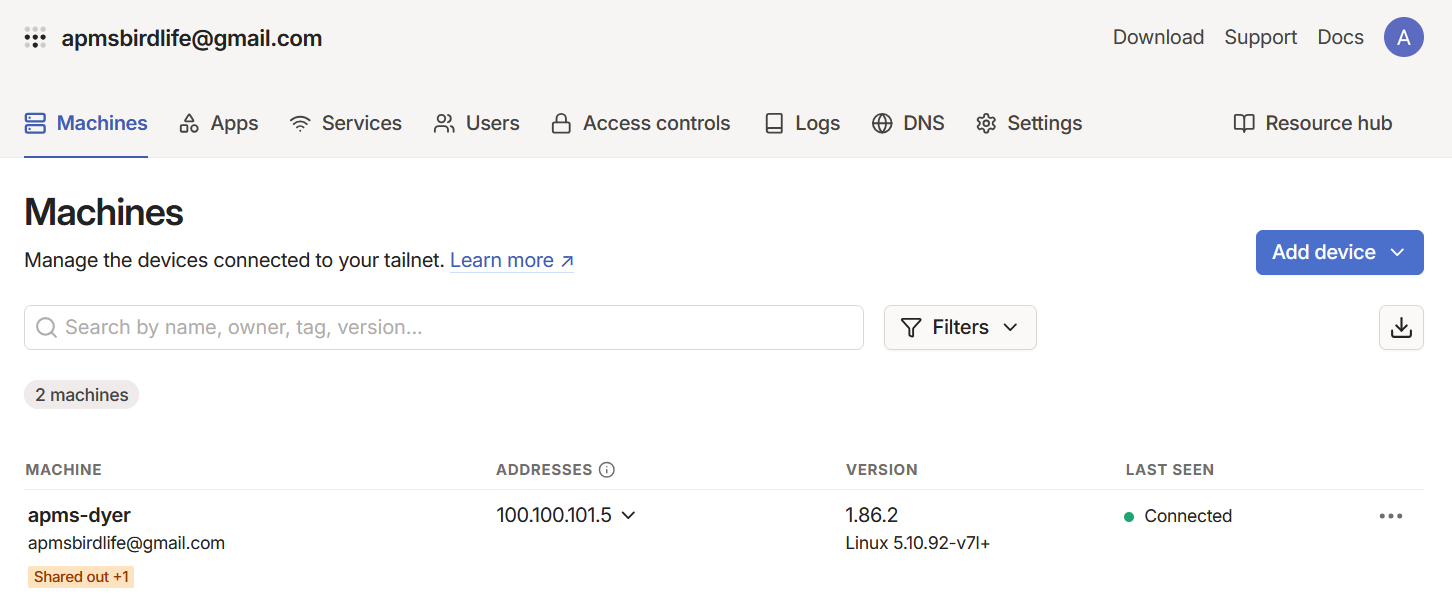
\includegraphics[width=6.25in,height=\textheight,keepaspectratio]{images/media/49_tailscale_admin.png}

}

\caption{\textbf{Figure 49.} Tailscale Admin Console.}

\end{figure}%

\begin{itemize}
\tightlist
\item
  Sharing a device with co-workers can be done by hovering your mouse
  over the machine you wish to share and then clicking on `Share' (Fig.
  50). Type in the email address you want to share it with and then
  send. Your co-worker should have tailscale installed on their laptop
  and then once they're ready, open the email that you sent to them and
  follow the instructions to add the device to their tailnet.
\end{itemize}

\begin{figure}[H]

{\centering \pandocbounded{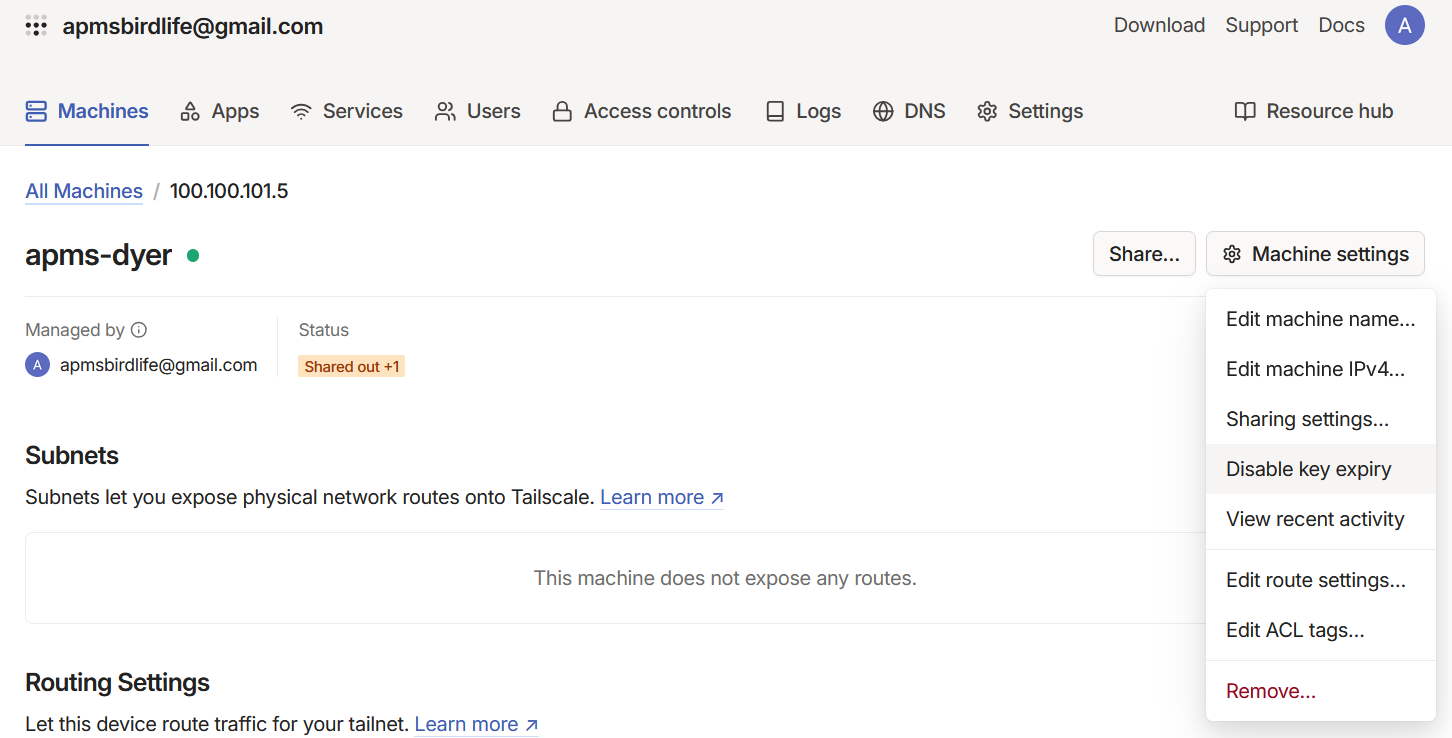
\includegraphics[keepaspectratio]{images/media/49_tailscale_sharing.png}}

}

\caption{\textbf{Figure 50.} Sharing access to a APMS with colleagues.}

\end{figure}%

\begin{itemize}
\item
  In the `Admin Console' click on the device you added to your tailnet
  and then on the right, click `\emph{Machine Settings}' and navigate
  down to `\emph{Disable key expiry}' and select it. This will allow
  your key to remain active indefinitely (as opposed to expiring after 6
  months).
\item
  You should now be ready to SSH into the raspberry pi from your laptop.
  Open the terminal and run: ssh apms@. For example: ssh
  apms@100.100.101.5
\end{itemize}

\section{Managing Background Services with
tmux}\label{managing-background-services-with-tmux}

When managing Raspberry Pi devices remotely, closing your terminal
window will normally terminate any active commands. To keep your
monitoring sessions open in the background, use \texttt{tmux} (Terminal
Multiplexer). This is especially useful for tracking system logs without
losing your place.

For instance, you can use \texttt{journalctl} to monitor your scales and
RFID services simultaneously and continuously:

\begin{Shaded}
\begin{Highlighting}[]
\CommentTok{\# Monitor scales and RFID services in real{-}time}
\FunctionTok{sudo}\NormalTok{ journalctl }\AttributeTok{{-}u}\NormalTok{ scales.service }\AttributeTok{{-}u}\NormalTok{ rfid.service }\AttributeTok{{-}f}
\end{Highlighting}
\end{Shaded}

If you want to only view one of the services, e.g.~just the scales
script, run the following:

\begin{Shaded}
\begin{Highlighting}[]
\FunctionTok{sudo}\NormalTok{ journalctl }\AttributeTok{{-}fu}\NormalTok{ scales}
\end{Highlighting}
\end{Shaded}

\begin{center}\rule{0.5\linewidth}{0.5pt}\end{center}

\subsection{Managing tmux Sessions}\label{managing-tmux-sessions}

Use the following commands to create, view, and manage your background
sessions.

\subsubsection{Start a New Session}\label{start-a-new-session}

To start a new session, it is best to give it a descriptive name
(e.g.~stony-monitor):

\begin{Shaded}
\begin{Highlighting}[]
\ExtensionTok{tmux}\NormalTok{ new }\AttributeTok{{-}s}\NormalTok{ stony{-}monitor}
\end{Highlighting}
\end{Shaded}

\subsubsection{List Available Sessions}\label{list-available-sessions}

To see all \texttt{tmux} sessions currently running on the Raspberry Pi:

\begin{Shaded}
\begin{Highlighting}[]
\ExtensionTok{tmux}\NormalTok{ ls}
\end{Highlighting}
\end{Shaded}

\subsubsection{Attach to an Existing
Session}\label{attach-to-an-existing-session}

If you get disconnected, reconnect to the Pi via SSH and resume your
session:

\begin{Shaded}
\begin{Highlighting}[]
\ExtensionTok{tmux}\NormalTok{ a }\AttributeTok{{-}t}\NormalTok{ stony{-}monitor}
\CommentTok{\# OR}
\ExtensionTok{tmux}\NormalTok{ attach }\CommentTok{\#if only one session is running}
\end{Highlighting}
\end{Shaded}

\subsubsection{Kill a Session}\label{kill-a-session}

When you are completely finished and want to close the session entirely:

\begin{Shaded}
\begin{Highlighting}[]
\ExtensionTok{tmux}\NormalTok{ kill{-}session }\AttributeTok{{-}t}\NormalTok{ stony{-}monitor}
\end{Highlighting}
\end{Shaded}

\begin{center}\rule{0.5\linewidth}{0.5pt}\end{center}

\begin{tcolorbox}[enhanced jigsaw, left=2mm, toptitle=1mm, breakable, opacitybacktitle=0.6, title=\textcolor{quarto-callout-tip-color}{\faLightbulb}\hspace{0.5em}{Essential tmux Shortcuts}, colback=white, opacityback=0, rightrule=.15mm, leftrule=.75mm, colbacktitle=quarto-callout-tip-color!10!white, bottomtitle=1mm, titlerule=0mm, coltitle=black, colframe=quarto-callout-tip-color-frame, arc=.35mm, bottomrule=.15mm, toprule=.15mm]

All \texttt{tmux} commands start with a prefix key combination:
\texttt{CTRL\ +\ b}. Press and release the prefix keys first, then press
the shortcut key.

\begin{itemize}
\tightlist
\item
  \textbf{Detach from Session}\\
  Hold \texttt{CTRL} and press \texttt{b} \(\rightarrow\) Release keys
  \(\rightarrow\) Press \texttt{d}
\item
  \textbf{Split Screen Vertically}\\
  Hold \texttt{CTRL} and press \texttt{b} \(\rightarrow\) Release keys
  \(\rightarrow\) Press \texttt{\%}
\item
  \textbf{Split Screen Horizontally}\\
  Hold \texttt{CTRL} and press \texttt{b} \(\rightarrow\) Release keys
  \(\rightarrow\) Press \texttt{"}
\item
  \textbf{Create New Window}\\
  Hold \texttt{CTRL} and press \texttt{b} \(\rightarrow\) Release keys
  \(\rightarrow\) Press \texttt{c}
\item
  \textbf{Close Window Pane}\\
  Hold \texttt{CTRL} and press \texttt{b} \(\rightarrow\) Release keys
  \(\rightarrow\) Press \texttt{x}
\item
  \textbf{Switch to Next Window}\\
  Hold \texttt{CTRL} and press \texttt{b} \(\rightarrow\) Release keys
  \(\rightarrow\) Press \texttt{n}
\item
  \textbf{Enter ``Scrolling'' Mode}\\
  Hold \texttt{CTRL} and press \texttt{b} \(\rightarrow\) Release keys
  \(\rightarrow\) Press \texttt{{[}}\\
  \emph{(Press \texttt{q} to exit scrolling mode and return to the live
  prompt)}
\end{itemize}

\end{tcolorbox}

\section{Set up the USB Flash Drive}\label{set-up-the-usb-flash-drive}

A 64GB USB Flash drive is used as a backup for the APMS data. Every
morning, the data gets backed up to the flash drive, before being
transferred to the cloud. To configure Flash drive, a NTFS partition
must be created.

\begin{itemize}
\item
  SSH into the Pi as described earlier in this manual.
\item
  Insert the USB Flash drive into any of the available USB ports on the
  Pi.
\item
  Unmount the flash drive (if mounted):
\end{itemize}

\begin{Shaded}
\begin{Highlighting}[]
\FunctionTok{umount}\NormalTok{ /dev/sda1}
\end{Highlighting}
\end{Shaded}

\begin{itemize}
\item
  Run fdisk on the drive:

  \begin{itemize}
  \item
    Create a new empty DOS partition: press `o' and enter
  \item
    Create a new partition: press `n' and enter -- use all the default
    options
  \item
    Change partition type: press `t' and enter -- choose 7 -
    `HPFS/NTFS/exFAT'
  \item
    Save and exit: press `w' and enter
  \end{itemize}

\begin{Shaded}
\begin{Highlighting}[]
\FunctionTok{sudo}\NormalTok{ fdisk /dev/sda}
\end{Highlighting}
\end{Shaded}
\item
  Format disk:
\end{itemize}

\begin{Shaded}
\begin{Highlighting}[]
\FunctionTok{sudo}\NormalTok{ mkntfs }\AttributeTok{{-}f} \AttributeTok{{-}L} \StringTok{"apms\_backup"}\NormalTok{ /dev/sda1}
\end{Highlighting}
\end{Shaded}

\begin{itemize}
\tightlist
\item
  Create mounting point
\end{itemize}

\begin{Shaded}
\begin{Highlighting}[]
\FunctionTok{mkdir}\NormalTok{ /home/apms/flash}
\end{Highlighting}
\end{Shaded}

\begin{itemize}
\tightlist
\item
  Mount:
\end{itemize}

\begin{Shaded}
\begin{Highlighting}[]
\FunctionTok{sudo}\NormalTok{ mount /dev/sda1 /home/apms/flash}
\end{Highlighting}
\end{Shaded}

\begin{itemize}
\tightlist
\item
  To check the USB Flash drive has been properly mounted, run:
\end{itemize}

\begin{Shaded}
\begin{Highlighting}[]
\FunctionTok{df} \AttributeTok{{-}h}
\end{Highlighting}
\end{Shaded}

\begin{itemize}
\tightlist
\item
  Partition sda1 should be mounted at /home/apms/flash and should show
  the size of the drive (Fig. 51).
\end{itemize}

\begin{figure}[H]

{\centering 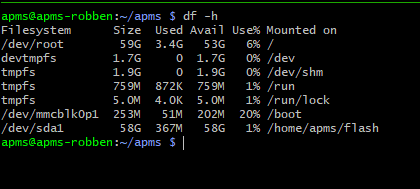
\includegraphics[width=6.25in,height=\textheight,keepaspectratio]{images/media/51_df_h.png}

}

\caption{\textbf{Figure 51.} Check if USB flash drive is mounted.}

\end{figure}%

\section{Turn off automatic time
updating}\label{turn-off-automatic-time-updating}

To prevent the Raspberry Pi from updating its system clock at an
inopportune time, automatic time updating must be disabled. A script
called \texttt{update\_system\_time.py} will handle the updating of the
system time. (See the section:
\hyperref[Setux5cux2520upux5cux2520theux5cux2520Crontab]{Set up the
Crontab} for more details).

\begin{itemize}
\item
  SSH into the Pi as described earlier in this manual.
\item
  To stop time-sync process, run:
\end{itemize}

\begin{Shaded}
\begin{Highlighting}[]
\FunctionTok{sudo}\NormalTok{ systemctl stop systemd{-}timesyncd}
\end{Highlighting}
\end{Shaded}

\begin{itemize}
\tightlist
\item
  To prevent the process from starting at boot, run:
\end{itemize}

\begin{Shaded}
\begin{Highlighting}[]
\FunctionTok{sudo}\NormalTok{ systemctl disable systemd{-}timesyncd}
\end{Highlighting}
\end{Shaded}

\begin{itemize}
\tightlist
\item
  To check it is indeed off, run:
\end{itemize}

\begin{Shaded}
\begin{Highlighting}[]
\FunctionTok{sudo}\NormalTok{ systemctl status systemd{-}timesyncd}
\end{Highlighting}
\end{Shaded}

\begin{itemize}
\tightlist
\item
  It is important to ensure that \emph{``update\_system\_time.py''} is
  set up to configure the time
\end{itemize}

\begin{figure}[H]

{\centering 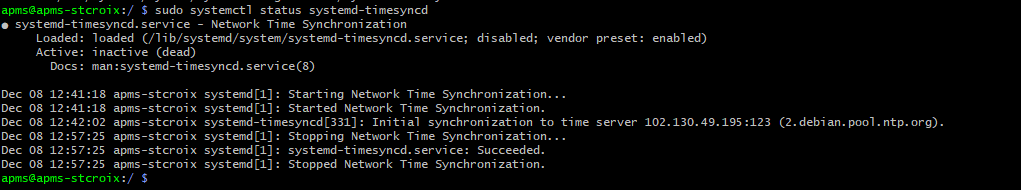
\includegraphics[width=7.29167in,height=\textheight,keepaspectratio]{images/media/52_systemd_timesyncd.png}

}

\caption{\textbf{Figure 52.} Confirm that the systemd-timesyncd is
inactive.}

\end{figure}%

\section{Disable Serial Console}\label{disable-serial-console}

The Raspberry Pi communicates with the Monitor via serial, using GPIO14
and GPIO15. The Raspberry Pi Serial Console must be disabled to allow
this serial port to be used:

\begin{itemize}
\tightlist
\item
  Run the following:
\end{itemize}

\begin{Shaded}
\begin{Highlighting}[]
\FunctionTok{sudo}\NormalTok{ raspi{-}config}
\end{Highlighting}
\end{Shaded}

\begin{itemize}
\item
  Select ``\textbf{Interfaces}''
\item
  Select ``\textbf{Serial Port}''
\item
  Select ``\textbf{NO}'' to login shell
\item
  Select ``\textbf{YES}'' to enable serial support
\item
  Save and exit
\end{itemize}

\section{Configure UART3}\label{configure-uart3}

UART3 is used to program the Arduino Monitor.

Enable serial port for programming by adding the following:

\begin{itemize}
\tightlist
\item
  Edit /boot/config.txt:
\end{itemize}

\begin{Shaded}
\begin{Highlighting}[]
\FunctionTok{sudo}\NormalTok{ nano /boot/config.txt}
\end{Highlighting}
\end{Shaded}

\begin{itemize}
\item
  Add ``\textbf{dtoverlay=uart3}'' after ``\textbf{enable\_uart=1}''
\item
  Save the file and exit. (Hold CTRL and press x - Then press `y' to
  save - then press Enter to exit)
\item
  Reboot:
\end{itemize}

\begin{Shaded}
\begin{Highlighting}[]
\FunctionTok{sudo}\NormalTok{ reboot}
\end{Highlighting}
\end{Shaded}

\section{Configure GPIO3 for Power
ON/OFF}\label{configure-gpio3-for-power-onoff}

To enable GPIO3 to be used to power the Raspberry Pi on/off, the config
file must be edited:

\begin{itemize}
\tightlist
\item
  Edit the config file. Run:
\end{itemize}

\begin{Shaded}
\begin{Highlighting}[]
\FunctionTok{sudo}\NormalTok{ nano /boot/config.txt}
\end{Highlighting}
\end{Shaded}

\begin{itemize}
\item
  Add ``\textbf{dtoverlay=gpio-shutdown}'' to the bottom of the file.
\item
  Save the file and exit. (Hold CTRL and press x - Then press `y' to
  save - then press Enter to exit)
\item
  Reboot:
\end{itemize}

\begin{Shaded}
\begin{Highlighting}[]
\FunctionTok{sudo}\NormalTok{ reboot}
\end{Highlighting}
\end{Shaded}

\section{Configure Git and Download
Firmware}\label{configure-git-and-download-firmware}

\begin{itemize}
\item
  SSH into the Pi as described earlier in this manual.
\item
  Install git (If you have not installed it already):
\end{itemize}

\begin{Shaded}
\begin{Highlighting}[]
\FunctionTok{sudo}\NormalTok{ apt{-}get install git}
\end{Highlighting}
\end{Shaded}

\begin{itemize}
\tightlist
\item
  Configure git:
\end{itemize}

\begin{Shaded}
\begin{Highlighting}[]
\FunctionTok{git}\NormalTok{ config }\AttributeTok{{-}{-}global}\NormalTok{ user.name }\StringTok{"apms"}
\FunctionTok{git}\NormalTok{ config }\AttributeTok{{-}{-}global}\NormalTok{ user.email }\OperatorTok{\textless{}}\NormalTok{apmsbirdlife@gmail.com}\OperatorTok{\textgreater{}}
\end{Highlighting}
\end{Shaded}

\begin{tcolorbox}[enhanced jigsaw, left=2mm, toptitle=1mm, breakable, opacitybacktitle=0.6, title=\textcolor{quarto-callout-tip-color}{\faLightbulb}\hspace{0.5em}{Tip}, colback=white, opacityback=0, rightrule=.15mm, leftrule=.75mm, colbacktitle=quarto-callout-tip-color!10!white, bottomtitle=1mm, titlerule=0mm, coltitle=black, colframe=quarto-callout-tip-color-frame, arc=.35mm, bottomrule=.15mm, toprule=.15mm]

All the firmware is stored on the
\href{https://www.github.com/apmsbirdlife/apms}{APMS BirdLife Github}
page.

\end{tcolorbox}

\begin{itemize}
\tightlist
\item
  Generate an SSH key pair:
\end{itemize}

\begin{Shaded}
\begin{Highlighting}[]
\FunctionTok{ssh{-}keygen} \AttributeTok{{-}t}\NormalTok{ rsa }\AttributeTok{{-}b}\NormalTok{ 4096 }\AttributeTok{{-}C}\NormalTok{ apmsbirdlife@gmail.com}
\end{Highlighting}
\end{Shaded}

\begin{itemize}
\item
  Press Enter for any questions that appear.
\item
  Start SSH agent:
\end{itemize}

\begin{Shaded}
\begin{Highlighting}[]
\BuiltInTok{eval} \VariableTok{$(}\FunctionTok{ssh{-}agent} \AttributeTok{{-}s}\VariableTok{)}
\end{Highlighting}
\end{Shaded}

\begin{itemize}
\tightlist
\item
  Add the private key to the agent to manage keys:
\end{itemize}

\begin{Shaded}
\begin{Highlighting}[]
\FunctionTok{ssh{-}add}\NormalTok{ \textasciitilde{}/.ssh/id\_rsa}
\end{Highlighting}
\end{Shaded}

\begin{itemize}
\item
  If you are one of the admins for the APMS BirdLife GitHub page, then
  go to \href{http://www.github.com}{GitHub} and log in using the
  details provided above.

  \begin{itemize}
  \item
    Click on the user image (top right of the page) and choose
    ``\textbf{Settings}''.

    \begin{itemize}
    \item
      ``\textbf{Settings}'' → ``\textbf{SSH and GPG keys}'' → Click on
      ``\textbf{New SSH key}''
    \item
      Under ``\textbf{Title}'', put ``APMS {[}site\_name{]}'' Example:
      ``APMS St Croix''. If replacing a pi, delete the previous one
      first.
    \end{itemize}
  \end{itemize}
\item
  In the ``\textbf{Key}'' field, copy the contents of the following
  file: \texttt{\textasciitilde{}/.ssh/id\_rsa.pub}. To do this, run the
  command:
\end{itemize}

\begin{Shaded}
\begin{Highlighting}[]
\FunctionTok{cat}\NormalTok{ \textasciitilde{}/.ssh/id\_rsa.pub}
\end{Highlighting}
\end{Shaded}

\begin{itemize}
\item
  Click ``\textbf{Add SSH Key}'' .
\item
  Go back to the Raspberry Pi terminal and authenticate:
\end{itemize}

\begin{Shaded}
\begin{Highlighting}[]
\FunctionTok{ssh} \AttributeTok{{-}T}\NormalTok{ git@github.com}
\end{Highlighting}
\end{Shaded}

\begin{verbatim}
- Type "yes" if asked to continue.
\end{verbatim}

\begin{itemize}
\tightlist
\item
  Go to the home folder and clone the repository:
\end{itemize}

\begin{Shaded}
\begin{Highlighting}[]
\BuiltInTok{cd}\NormalTok{ \textasciitilde{}}
\FunctionTok{git}\NormalTok{ clone git@github.com:apmsbirdlife/apms.git}


\ExtensionTok{{-}}\NormalTok{   All the APMS firmware should now be downloaded to }\KeywordTok{\textasciigrave{}}\ExtensionTok{\textasciitilde{}/apms/.}\KeywordTok{\textasciigrave{}}\NormalTok{ Go to the directory, then make sure you are on the correct branch: }
\KeywordTok{\textasciigrave{}\textasciigrave{}\textasciigrave{}}\FunctionTok{bash}
\BuiltInTok{cd}\NormalTok{ \textasciitilde{}/apms}
\FunctionTok{git}\NormalTok{ checkout main}
\end{Highlighting}
\end{Shaded}

\begin{itemize}
\tightlist
\item
  To update to the latest firmware, go to
  \texttt{\textasciitilde{}/apms/} and run:
\end{itemize}

\begin{Shaded}
\begin{Highlighting}[]
\FunctionTok{git}\NormalTok{ pull}
\end{Highlighting}
\end{Shaded}

\section{Finding the RS485 Serial
Numbers}\label{finding-the-rs485-serial-numbers}

Each scale is connected to the Raspberry Pi via a RS485 converter. Each
converter has a unique serial number and that is how the Pi can
determine which scale is which. This is why it is important to label the
indicator, scale and RS485 converter as ``scale 1'' or ``scale 2''.
These should not be mixed and matched once the system has been set up.

\begin{itemize}
\tightlist
\item
  To identify the serial number of each converter, a simple script was
  created. The script will be run twice, once for each converter. Run
  the script and follow the on-screen instructions:
\end{itemize}

\begin{Shaded}
\begin{Highlighting}[]
\NormalTok{python3 }\OperatorTok{\textasciitilde{}/}\NormalTok{apms}\OperatorTok{/}\NormalTok{tools}\OperatorTok{/}\NormalTok{find\_rs485\_serial\_number.py}
\end{Highlighting}
\end{Shaded}

\begin{itemize}
\tightlist
\item
  Note down the serial number for each converter as it will be used when
  configuring the APMS. See
  \hyperref[Configuringux5cux2520theux5cux2520APMS]{Configuring the
  APMS}.
\end{itemize}

\section{Configuring the APMS}\label{configuring-the-apms}

\begin{itemize}
\item
  All the parameters that can and must be set for the system to work
  properly can be found in the config file:
  \texttt{\textasciitilde{}/apms/config.json}
\item
  A new system needs a config file to be created, an existing system
  will already have the file.
\item
  To check if the config file already exists, list the contents of the
  apms directory and see if the file is present:
\end{itemize}

\begin{Shaded}
\begin{Highlighting}[]
\FunctionTok{ls}\NormalTok{ \textasciitilde{}/apms/}
\end{Highlighting}
\end{Shaded}

\begin{itemize}
\tightlist
\item
  If a config file already exists, it can be edited with:
\end{itemize}

\begin{Shaded}
\begin{Highlighting}[]
\FunctionTok{sudo}\NormalTok{ nano \textasciitilde{}/apms/config.json}
\end{Highlighting}
\end{Shaded}

Save the file and exit. (Hold \textbf{CTRL} and press \textbf{x} -- Then
press `\textbf{y}' to save -- then press Enter to exit)

\begin{itemize}
\item
  For a new system, the file \texttt{config\_template.json} can be used.

  \begin{itemize}
  \tightlist
  \item
    Make a copy of the template:
  \end{itemize}

\begin{Shaded}
\begin{Highlighting}[]
\FunctionTok{cp}\NormalTok{ \textasciitilde{}/apms/config\_template.json \textasciitilde{}/apms/config.json}
\end{Highlighting}
\end{Shaded}

  \begin{itemize}
  \tightlist
  \item
    To edit the config file, run:
  \end{itemize}

\begin{Shaded}
\begin{Highlighting}[]
\FunctionTok{sudo}\NormalTok{ nano \textasciitilde{}/apms/config.json}
\end{Highlighting}
\end{Shaded}

  \begin{itemize}
  \tightlist
  \item
    Refer to the table below when editing the config file. \ul{The
    values given in bold are defaults and do not need to be changed.}
  \end{itemize}
\end{itemize}

The table below shows the parameters and their descriptions.

\begin{longtable}[]{@{}
  >{\raggedright\arraybackslash}p{(\linewidth - 2\tabcolsep) * \real{0.5000}}
  >{\raggedright\arraybackslash}p{(\linewidth - 2\tabcolsep) * \real{0.5000}}@{}}
\toprule\noalign{}
\begin{minipage}[b]{\linewidth}\raggedright
Parameter
\end{minipage} & \begin{minipage}[b]{\linewidth}\raggedright
Description
\end{minipage} \\
\midrule\noalign{}
\endhead
\bottomrule\noalign{}
\endlastfoot
\textbf{SITE\_NAME} & Unique site name. All lowercase, no spaces.
Example: \texttt{"stony\_point"} \\
\textbf{SITE\_CODE} & Unique 3-letter site code. All capital letters.
Example: \texttt{"STO"} for Stony. \\
\textbf{SCALE\_1\_SERIAL\_NUMBER} & Unique serial number for the first
RS485 converter. See:
\hyperref[Findingux5cux2520theux5cux2520RS485ux5cux2520Serialux5cux2520Numbers]{Finding
the RS485 Serial Numbers} \\
\textbf{SCALE\_2\_SERIAL\_NUMBER} & Unique serial number for the second
RS485 converter. See:
\hyperref[Findingux5cux2520theux5cux2520RS485ux5cux2520Serialux5cux2520Numbers]{Finding
the RS485 Serial Numbers} \\
\textbf{AWS\_S3\_DATA\_PATH} & This should be
\texttt{"s3://apmsbirdlife/APMS/data/{[}site\ name{]}/"}. Example:
\texttt{*"s3://apmsbirdlife/APMS/data/stony\_point/"*} \\
\textbf{AWS\_ACCESS\_KEY} & The access key you obtained when the user
was created. See
\hyperref[Creatingux5cux2520aux5cux2520Userux5cux2520onux5cux2520AWSux5cux2520S3]{Creating
a User on AWS S3} \\
\textbf{AWS\_SECRET\_ACCESS\_KEY} & The secret access key you obtained
when the user was created. See
\hyperref[Creatingux5cux2520aux5cux2520Userux5cux2520onux5cux2520AWSux5cux2520S3]{Creating
a User on AWS S3} \\
\textbf{AWS\_BUCKET} & Name of AWS S3 Bucket:
\textbf{``apmsbirdlife''} \\
\textbf{APMS\_ABS\_PATH} & Absolute path where APMS is installed:
\textbf{``/home/apms/''} \\
\textbf{DATA\_PATH} & Path where raw data is stored:
\textbf{``/home/apms/data/''} \\
\textbf{LOGS\_PATH} & Path where log files are stored:
\textbf{``/home/apms/logs/''} \\
\textbf{ERROR\_PATH} & Path where error files are stored:
\textbf{``/home/apms/error/''} \\
\textbf{USB\_PATH} & Path when USB Flash drive is mounted:
\textbf{``/home/apms/flash/''} \\
\textbf{USB\_PARTITION} & USB Flash drive partition:
\textbf{``/dev/sda1''} \\
\textbf{EMAIL\_ADDRESS} & APMS main email address:
\textbf{``apmsbirdlife@gmail.com''} \\
\textbf{EMAIL\_PASSWORD} & This is the password to the main email
address: \textbf{``dayammxlcvvwmdza''} \\
\textbf{EMAIL\_ADDRESS\_ADMIN} & Email address of APMS administrator:
\textbf{``philip.faure@birdlife.org.za''} \\
\textbf{SCALE\_SAMPLING\_FREQ} & Sampling frequency of scales (samples
per second): \textbf{100} \\
\textbf{SCALE\_BAUD\_RATE} & RS485 Serial Converter BAUD rate:
\textbf{115200} \\
\textbf{MIN\_PENGUIN\_WEIGHT} & This is the minimum penguin weight (in
kg) expected to be encountered in the field: \textbf{1.9} \\
\textbf{MAX\_PENGUIN\_WEIGHT} & This is the maximum penguin weight (in
kg) expected to be encountered in the field: \textbf{4.3} \\
\textbf{MAX\_DEAD\_WEIGHT} & Maximum weight allowed (in kg) for
sand/debris on the scales before warning: \textbf{0.5} \\
\textbf{SCALE\_EMPTY\_TIME} & Duration (in seconds) the scales must be
empty before the event stops: \textbf{3} \\
\textbf{RFID\_SERIAL\_NUMBER} & This is the serial number of the serial
converter inside the BioMark RFID reader: \textbf{``0001''} \\
\textbf{RFID\_BAUD\_RATE} & This is the BAUD rate of the BioMark serial
converter: \textbf{115200} \\
\textbf{SERIAL\_PORT\_INTERNAL} & This is the name of the serial port
used for communication with the Monitor: \textbf{``/dev/ttyS0''} \\
\textbf{INTERNAL\_BAUD\_RATE} & This is the BAUD rate for communication
between the Pi and the Monitor: \textbf{115200} \\
\textbf{MAX\_SCALE\_ERROR\_COUNT} & This is the number of times a scale
can fail before it gets disabled: \textbf{3} \\
\textbf{CPU\_TEMP\_WARNING} & CPU temperature (in °C) at which to send
out warning message: \textbf{60} \\
\textbf{CPU\_TEMP\_DANGER} & CPU temperature (in °C) at which Raspberry
Pi will start throttling the CPU: \textbf{70} \\
\textbf{UPLOAD\_HOUR} & Hour of day to do the data transfer to the
cloud. 1 = 1:00, 19 = 7pm etc: \textbf{1} \\
\textbf{UPLOAD} & This variable is set to \textbf{1} to allow daily data
uploads to the cloud (0 to disable): \textbf{1} \\
\end{longtable}

\begin{itemize}
\item
  After editing, Save the file and exit.

  \begin{itemize}
  \tightlist
  \item
    Hold \textbf{CTRL} and press \textbf{x}. Then press `\textbf{y}' to
    save, then press Enter to exit
  \end{itemize}
\item
  The configuration file has now been created.
\end{itemize}

\pandocbounded{\includegraphics[keepaspectratio]{images/media/.pdf}}

\chapter{Programming the Arduino Monitor via the
Pi}\label{programming-the-arduino-monitor-via-the-pi}

As discussed in \hyperref[UPDIux5cux2520Programming]{UPDI Programming},
the Arduino is programmed via UPDI.

\section{Initial Setup}\label{initial-setup}

\begin{itemize}
\item
  Before soldering the link and connecting the UPDI wire, compile and
  upload the test sketch as discussed in
  \hyperref[Programmingux5cux2520viaux5cux2520theux5cux2520Arduinoux5cux2520Software]{Programming
  via the Arduino Software}.
\item
  Ensure the Monitor Circuit Board has been fully tested before plugging
  it into the Pi. See
  \hyperref[Testingux5cux2520theux5cux2520Monitorux5cux2520Circuitux5cux2520Board]{Testing
  the Monitor Circuit Board}.
\item
  Ensure the Serial Console has been disabled as discussed in
  \hyperref[Disableux5cux2520Serialux5cux2520Console]{Disable Serial
  Console}.
\item
  Ensure UART3 has been configured as discussed in
  \hyperref[Configureux5cux2520UART3]{Configure UART3}.
\item
  Ensure GPIO3 has been configured to power the Raspberry Pi on/off as
  discussed in
  \hyperref[Configureux5cux2520GPIO3ux5cux2520forux5cux2520Powerux5cux2520ONux2fOFF]{Configure
  GPIO3 for Power ON/OFF}.
\item
  Provide 24V DC to the Main Unit, providing power for the Raspberry Pi
  and Arduino to boot up.
\item
  SSH into the Pi.
\item
  Ensure the latest firmware has been downloaded:
\end{itemize}

\begin{Shaded}
\begin{Highlighting}[]
\BuiltInTok{cd}\NormalTok{ \textasciitilde{}/apms}
\FunctionTok{git}\NormalTok{ clone}
\end{Highlighting}
\end{Shaded}

\begin{itemize}
\tightlist
\item
  To compile the firmware, arduino-cli must be installed. Run:
\end{itemize}

\begin{Shaded}
\begin{Highlighting}[]
\BuiltInTok{cd}\NormalTok{ \textasciitilde{}}
\ExtensionTok{curl} \AttributeTok{{-}fsSL}\NormalTok{ https://raw.githubusercontent.com/arduino/arduino{-}cli/master/install.sh }\KeywordTok{|} \FunctionTok{sh}
\end{Highlighting}
\end{Shaded}

Add to path:

\begin{itemize}
\tightlist
\item
  Edit bashrc:
\end{itemize}

\begin{Shaded}
\begin{Highlighting}[]
\FunctionTok{nano}\NormalTok{ \textasciitilde{}/.bashrc}
\end{Highlighting}
\end{Shaded}

\begin{itemize}
\item
  Add the following to the bottom:
  \texttt{export\ PATH=\textbackslash{}\$PATH:/home/apms/bin}
\item
  Save the file and exit. (Hold \textbf{CTRL} and press \textbf{x} --
  Then press `\textbf{y}' to save -- then press Enter to exit)
\item
  Type:
\end{itemize}

\begin{Shaded}
\begin{Highlighting}[]
\BuiltInTok{source}\NormalTok{ \textasciitilde{}/.bashrc}
\end{Highlighting}
\end{Shaded}

To install the AVR core, run:

\begin{Shaded}
\begin{Highlighting}[]
\ExtensionTok{arduino{-}cli}\NormalTok{ core install arduino:megaavr}
\end{Highlighting}
\end{Shaded}

To set up the config file, run:

\begin{Shaded}
\begin{Highlighting}[]
\ExtensionTok{arduino{-}cli}\NormalTok{ config init}
\end{Highlighting}
\end{Shaded}

The Software Serial port buffer must be increased:

\begin{itemize}
\tightlist
\item
  Determine the version number. Run:
\end{itemize}

\begin{Shaded}
\begin{Highlighting}[]
\FunctionTok{ls}\NormalTok{ \textasciitilde{}/.arduino15/packages/arduino/hardware/megaavr/}
\end{Highlighting}
\end{Shaded}

\begin{itemize}
\tightlist
\item
  The run the following:
\end{itemize}

\begin{Shaded}
\begin{Highlighting}[]
\FunctionTok{sudo}\NormalTok{ nano \textasciitilde{}/.arduino15/packages/arduino/hardware/megaavr/[VERSION NUMBER]/libraries/SoftwareSerial/src/SoftwareSerial.h}
\end{Highlighting}
\end{Shaded}

\begin{itemize}
\item
  Look for the line
  \texttt{\#define\ \_SS\_MAX\_RX\_BUFF\ 64\ //\ RX\ buffer\ size} and
  change 64 to 100
\item
  Save the file and exit. (Hold \textbf{CTRL} and press \textbf{x} --
  Then press \textbf{y} to save -- then press Enter to exit)
\end{itemize}

\section{Compiling and Uploading}\label{compiling-and-uploading}

\begin{itemize}
\item
  SSH into the Pi
\item
  Go to the Monitor firmware directory:
\end{itemize}

\begin{Shaded}
\begin{Highlighting}[]
\BuiltInTok{cd}\NormalTok{ \textasciitilde{}/apms/system\_monitor}
\end{Highlighting}
\end{Shaded}

\begin{itemize}
\tightlist
\item
  Compile the firmware:
\end{itemize}

\begin{Shaded}
\begin{Highlighting}[]
\FunctionTok{chmod}\NormalTok{ +x .compile.sh}
\FunctionTok{chmod}\NormalTok{ +x .upload.sh}
\ExtensionTok{./compile.sh}
\end{Highlighting}
\end{Shaded}

\begin{figure}[H]

{\centering 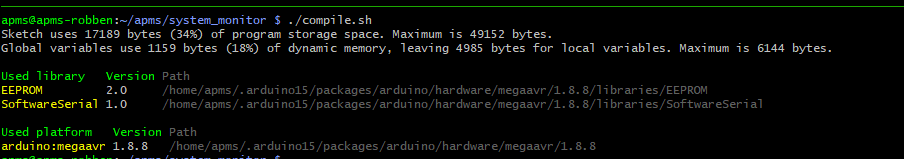
\includegraphics[width=7.29167in,height=\textheight,keepaspectratio]{images/media/53_compile_sh.png}

}

\caption{\textbf{Figure 53.} Compiling the firmware.}

\end{figure}%

\begin{itemize}
\tightlist
\item
  Upload the firmware to the monitor:
\end{itemize}

\begin{Shaded}
\begin{Highlighting}[]
\ExtensionTok{./upload.sh}
\end{Highlighting}
\end{Shaded}

\begin{itemize}
\item
  The output can be seen in the below screenshot.
\item
  If the upload fails, check the UPDI wire and link, Schottky diode and
  the wiring of the level shifter.
\item
  The Monitor should reboot and send an SMS to the operator.
\end{itemize}

\begin{figure}[H]

{\centering 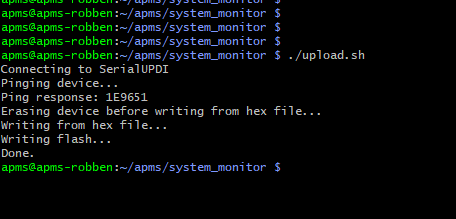
\includegraphics[width=6.25in,height=\textheight,keepaspectratio]{images/media/54_upload_sh.png}

}

\caption{\textbf{Figure 54.} Uploading the firmware.}

\end{figure}%

\chapter{BioMark Reader}\label{biomark-reader}

The BioMark RFID Reader is a device used to record penguins that have
been PIT-tagged. The device outputs the tag number via a serial-to-USB
converter, accessible via a mini-USB port on the device.

The reader has many different configurations and the latest BioMark
manual should always be followed.

\section{Overview}\label{overview-4}

Below is some information of the currently used model, for reference.
The Raspberry Pi reads the tags via a USB cable, plugged into the front
of the APMS Main Unit.

For the reader to operate, it needs 24V power and an RFID antenna
connected. For the pinout, see Fig. 55.

To make an antenna, see
\hyperref[Makingux5cux2520aux5cux2520BioMarkux5cux2520Antenna]{Making a
BioMark Antenna}. As of 2026, we have been using antenna's custom made
by BioMark to fit perfectly in between our scales.

\begin{figure}[H]

{\centering 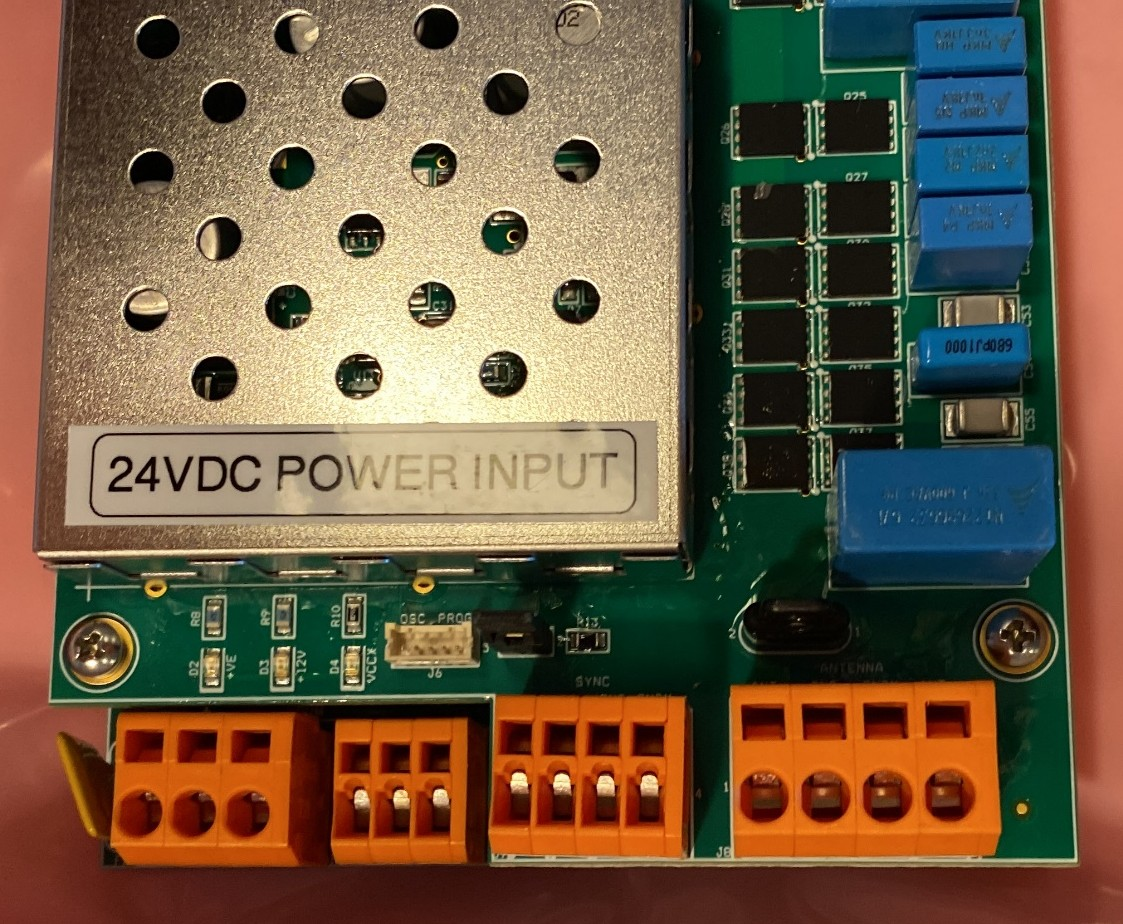
\includegraphics[width=6.25in,height=\textheight,keepaspectratio]{images/media/55_biomark.jpeg}

}

\caption{\textbf{Figure 55.} BioMark pinout.}

\end{figure}%

The BioMark reader can be configured either via the BioMark Software
(Device Manager) or via the Raspberry Pi terminal. Both methods
described here use a USB-A to mini-USB cable to connect to the Reader.

It is also possible to connect to reader via a RS232 or Bluetooth
connection. Refer to the BioMark documentation for more information if
this is required.

Application Firmware Version v 1.7.1

\section{Connect to BioMark via Device
Manager}\label{connect-to-biomark-via-device-manager}

\begin{itemize}
\item
  BioMark Device Manager, can be installed on a Windows PC to configure
  the system. Currently version 1.2.15.1 is being used and can be found
  on the S3 account or downloaded here:

  \begin{itemize}
  \tightlist
  \item
    \href{_book/files/DeviceManagerStandalone_1.2.15.1.zip}{Download
    Device Manager 1.2.15.1.zip}
  \end{itemize}
\item
  The Windows 10 and Windows 11 driver for the serial converter
  (\emph{CP210x\_Universal\_Windows\_Driver\_11.3.0}), used by the
  BioMark Reader, can be found on the S3 account or downloaded here:

  \begin{itemize}
  \tightlist
  \item
    \href{_book/files/CP210x_Universal_Windows_Driver_11.3.0.zip}{Download
    Windows Driver}
  \end{itemize}
\item
  Please refer to the IS1001 Reader User Manual and the Device Manager
  Software Manual for instructions on how to connect and configure the
  reader. Both can be found at:

  \begin{itemize}
  \item
    \href{_book/files/IS1001_Reader_User_Manual_Rev_11.pdf}{Download
    IS1001 Reader User Manual}
  \item
    \href{_book/files/Device-Manager-Software-Manual-v1.1.pdf}{Download
    Device Software Manual}
  \end{itemize}
\item
  Refer to the section
  \hyperref[Configuringux5cux2520theux5cux2520BioMarkux5cux2520Reader]{Configuring
  the BioMark Reader} for the required settings.
\end{itemize}

\section{Connect to BioMark via Raspberry Pi
Terminal}\label{connect-to-biomark-via-raspberry-pi-terminal}

\begin{itemize}
\item
  To connect to the BioMark Reader from the Raspberry Pi terminal,
  ensure that both the BioMark Reader and Raspberry Pi are powered up.
\item
  SSH into the Pi
\item
  Check that the RFID service is not running in the background and stop
  the service if it is:

  \begin{itemize}
  \tightlist
  \item
    Check with:
  \end{itemize}

\begin{Shaded}
\begin{Highlighting}[]
\ExtensionTok{systemctl}\NormalTok{ status rfid}
\end{Highlighting}
\end{Shaded}

  \begin{itemize}
  \tightlist
  \item
    If active, stop the service:
  \end{itemize}

\begin{Shaded}
\begin{Highlighting}[]
\FunctionTok{sudo}\NormalTok{ systemctl stop rfid}
\end{Highlighting}
\end{Shaded}
\item
  Connect the USB cable to the mini-USB port on the BioMark reader and
  to any of the USB ports of the Raspberry Pi. If an APMS Main Unit has
  been built, the front USB port can be used.
\item
  After the USB cable is plugged into the Pi, the BioMark serial
  converter will be assigned to a device file. This will either be
  ``ttyUSB0'', ``ttyUSB1'' or ``ttyUSB2'', depending on what other USB
  devices are plugged in. To determine which device file to use, run the
  rfid script:

\begin{Shaded}
\begin{Highlighting}[]
\ExtensionTok{python3}\NormalTok{ \textasciitilde{}/apms/rfid.py}
\end{Highlighting}
\end{Shaded}

  \begin{itemize}
  \tightlist
  \item
    Find the device file name as indicated in Fig. 56 below.
  \end{itemize}
\end{itemize}

\begin{figure}[H]

{\centering 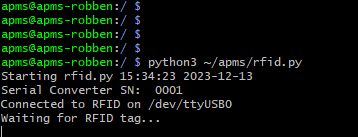
\includegraphics[width=6.25in,height=\textheight,keepaspectratio]{images/media/56_rfid_py.png}

}

\caption{\textbf{Figure 56.} Finding the device name using the Python
RFID script.}

\end{figure}%

\begin{itemize}
\item
  Close the script: Hold \textbf{CTRL} and press \textbf{c}
\item
  To connect to the BioMark reader from the Pi, a program called Minicom
  will be used. This was installed when the Raspberry Pi was set up. See
  \hyperref[Installux5cux2520applicationsux5cux2520andux5cux2520libraries]{Install
  applications and libraries}.

  \begin{itemize}
  \tightlist
  \item
    Run:
  \end{itemize}

\begin{Shaded}
\begin{Highlighting}[]
\ExtensionTok{minicom} \AttributeTok{{-}D}\NormalTok{ /dev/[device file]}
\end{Highlighting}
\end{Shaded}

\begin{verbatim}
-   Example: `minicom -D /dev/ttyUSB0`
\end{verbatim}

  \begin{itemize}
  \item
    Once inside minicom, disable ``Hardware Flow Control'':
  \item
    Hold \textbf{CTRL} and press \textbf{a} - Then press \textbf{o} to
    bring up the options menu, go to ``\textbf{Serial port setup}'' and
    press Enter. See screenshot below
  \end{itemize}
\end{itemize}

\begin{figure}[H]

{\centering 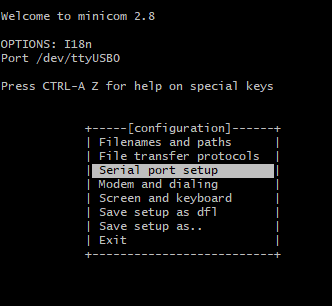
\includegraphics[width=6.25in,height=\textheight,keepaspectratio]{images/media/57_hardwareflowcontrol.png}

}

\caption{\textbf{Figure 57.} Turning off `Hardware Flow Control'.}

\end{figure}%

\begin{itemize}
\item
  Ensure ``Hardware Flow Control'' is off (It must have ``no'' next to
  it) - see Fig. 58.

  \begin{itemize}
  \tightlist
  \item
    If ``Hardware Flow Control'' is on, turn it off by pressing
    ``\textbf{f}''.
  \end{itemize}
\end{itemize}

\begin{figure}[H]

{\centering 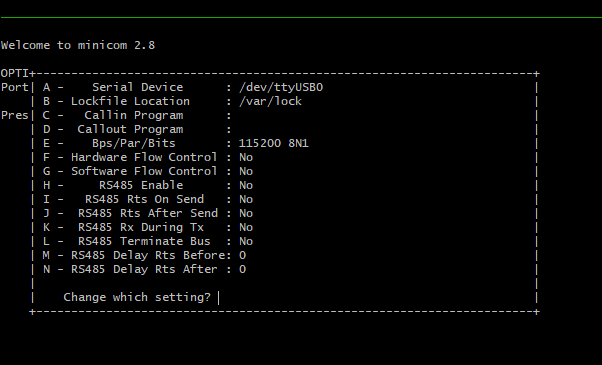
\includegraphics[width=6.25in,height=\textheight,keepaspectratio]{images/media/58_hardwareflowcontrol.png}

}

\caption{\textbf{Figure 58.} Hardware Flow Control disabled.}

\end{figure}%

\begin{itemize}
\item
  Press \textbf{Enter} to save and return to the Options menu.
\item
  Press \textbf{Esc} to exit the Options menu
\item
  Type ``\textbf{rfs}'' and press \textbf{Enter}. The current
  configuration should be printed to the screen.
\item
  You will not see the letters ``\textbf{rfs}'' until you press
  \textbf{Enter}.
\item
  An Example for Robben Island can be seen in Fig. 59.
\end{itemize}

\begin{figure}[H]

{\centering 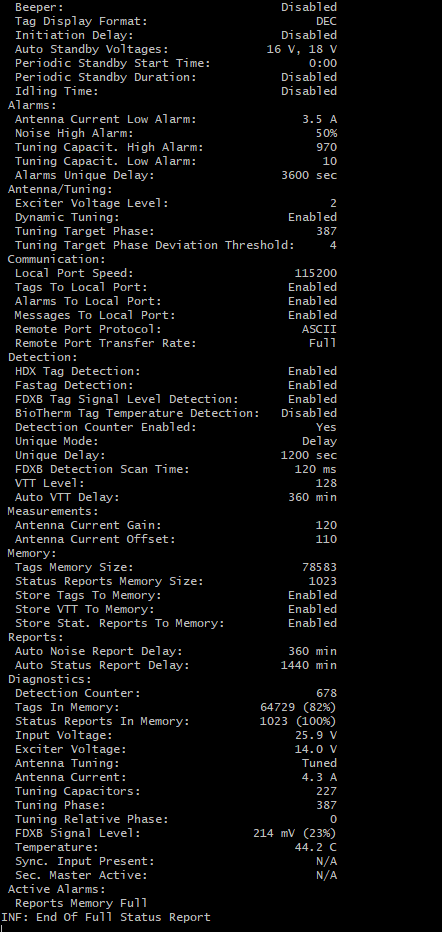
\includegraphics[width=6.25in,height=\textheight,keepaspectratio]{images/media/59_rfs.png}

}

\caption{\textbf{Figure 59.} RFS system configuration for Robben
Island.}

\end{figure}%

\begin{itemize}
\tightlist
\item
  If you see the configuration page as above, it means you have
  successfully connected to the BioMark Reader and can now send/receive
  commands in the console.
\end{itemize}

\section{Configuring the BioMark
Reader}\label{configuring-the-biomark-reader}

After successfully connecting to the BioMark Reader as discussed above,
the system can be configured.

\begin{itemize}
\item
  If using the ``Device Manager'' software, please refer the BioMark
  documentation and use the settings provided below.
\item
  If connecting via a Raspberry Pi terminal, use the commands below to
  set the BioMark parameters.
\item
  \textbf{Before executing any commands, it is always a good idea to run
  ``rfs'' and check that a status report is received. This confirms the
  reader is working properly and clears the serial buffer of any garbage
  characters that may be present.}
\end{itemize}

The settings given below are used for a BioMark Reader connected to an
APMS.

\begin{itemize}
\tightlist
\item
  If connecting to the BioMark Reader via the Raspberry Pi terminal
  (minicom), the commands given in the table below can be used to
  configure the system. Keep the default for all other settings. Compare
  the values in the table with the values obtained from executing
  ``rfs'', and change the settings as needed.
\end{itemize}

\begin{longtable}[]{@{}
  >{\raggedright\arraybackslash}p{(\linewidth - 4\tabcolsep) * \real{0.4400}}
  >{\raggedright\arraybackslash}p{(\linewidth - 4\tabcolsep) * \real{0.3333}}
  >{\raggedright\arraybackslash}p{(\linewidth - 4\tabcolsep) * \real{0.2000}}@{}}
\toprule\noalign{}
\begin{minipage}[b]{\linewidth}\raggedright
Setting
\end{minipage} & \begin{minipage}[b]{\linewidth}\raggedright
Value
\end{minipage} & \begin{minipage}[b]{\linewidth}\raggedright
Command
\end{minipage} \\
\midrule\noalign{}
\endhead
\bottomrule\noalign{}
\endlastfoot
Operation Mode & ``Scan'' & \textbf{ROM1} \\
Network Mode & IS1001 Standalone & \textbf{RNMS} \\
Exciter Sync. Mode & Standalone & \textbf{RSM0} \\
Beeper & Disabled & \textbf{RBS0} \\
Tag Display Format & DEC & \textbf{RDFD} \\
Exciter Voltage Level & 3 & \textbf{AVE3} \\
Dynamic Tuning & Enabled & \textbf{ADT1} \\
Tags To Local Port & Enabled & \textbf{CTL1} \\
Remote Port Protocol & ASCII & \textbf{CPRA} \\
Fastag Detection & Enabled & \textbf{DFH1} \\
Detection Counter Enabled & Yes & \textbf{DCS1} \\
Unique Mode & Delay & \textbf{DUMD} \\
Unique Delay & 1200 sec & \textbf{DUD1200} \\
Auto VTT Delay & 360 min & \textbf{DTD360} \\
\end{longtable}

\begin{itemize}
\item
  After changing all the necessary parameters, run ``rfs'' again to
  confirm all the settings are correct.
\item
  Take a test tag and move it close to the antenna. The tag should be
  picked up and displayed in minicom. If so, you have successfully
  configured the BioMark reader.
\item
  Exit minicom

  \begin{itemize}
  \tightlist
  \item
    Hold \textbf{CTRL} and press \textbf{a} - Then release keys - Then
    press `\textbf{q}' and then \textbf{Enter} to exit.
  \end{itemize}
\end{itemize}

\section{Making a BioMark Antenna}\label{making-a-biomark-antenna}

An experimental antenna has been made with some success. We no longer
use these antennas and all systems have been upgraded with a tailormade
antenna custom made for our system by BioMark. These custom made
antennas have a better detection range, are easier to tune, and won't
lose resonance if the cables are moved. To test a new antenna, first
ensure a connection to the BioMark Reader has been made, as discussed
previously.

As the wire being used might be slightly different, the basic method
will be described below. The antennas at Dyer Island and Robben Island
were made using the same 3-core wire as used to run power from the solar
supply to the APMS. The main idea behind making an antenna is to make
multiple loops and cutting it down to the correct length to achieve
resonance.

\begin{itemize}
\tightlist
\item
  Start with a length of wire, L, strip both ends and connect the wires
  as shown in Fig. 60.
\end{itemize}

\begin{figure}[H]

{\centering 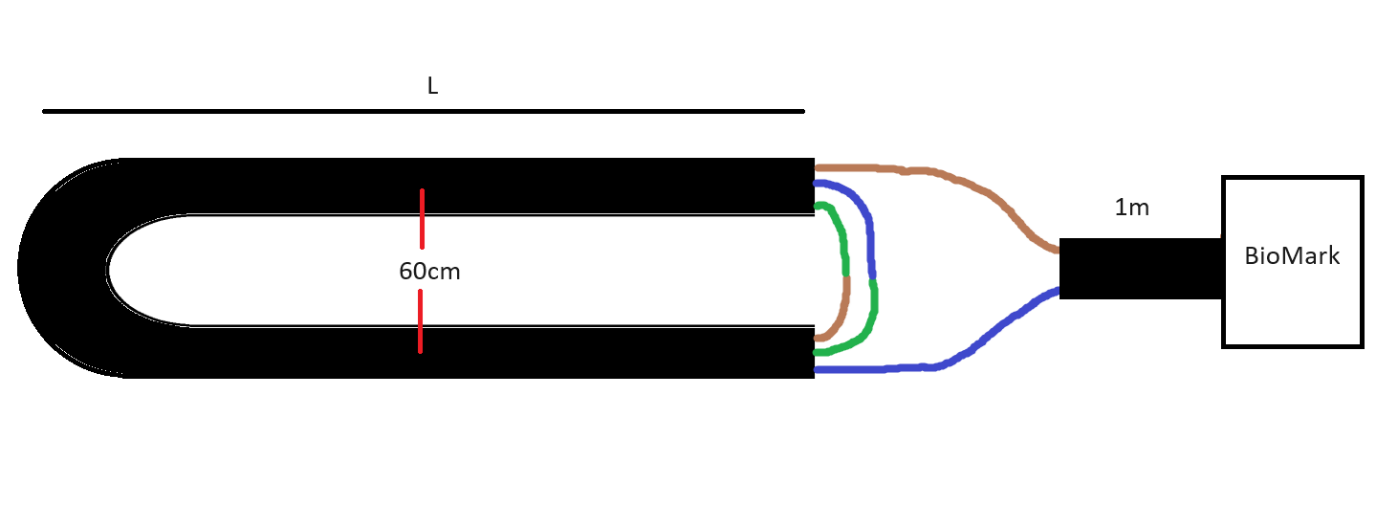
\includegraphics[width=7.29167in,height=\textheight,keepaspectratio]{images/media/60_antenna.png}

}

\caption{\textbf{Figure 60.} Cable layout when making an antenna.}

\end{figure}%

\begin{itemize}
\item
  The length to start at is a bit of a guess. The three core wire used
  for the latest antennas ended up being approximately 15-16 m. Thicker
  wires or more loops will result in a shorter length.
\item
  Add a ``fly-lead'' of approximately 1m to join the antenna and the
  BioMark reader.
\item
  During the test, lay the wires parallel, 40-60 cm apart, and connect
  the antenna to the BioMark reader. See Fig. 61 as an example.
\end{itemize}

\begin{figure}[H]

{\centering 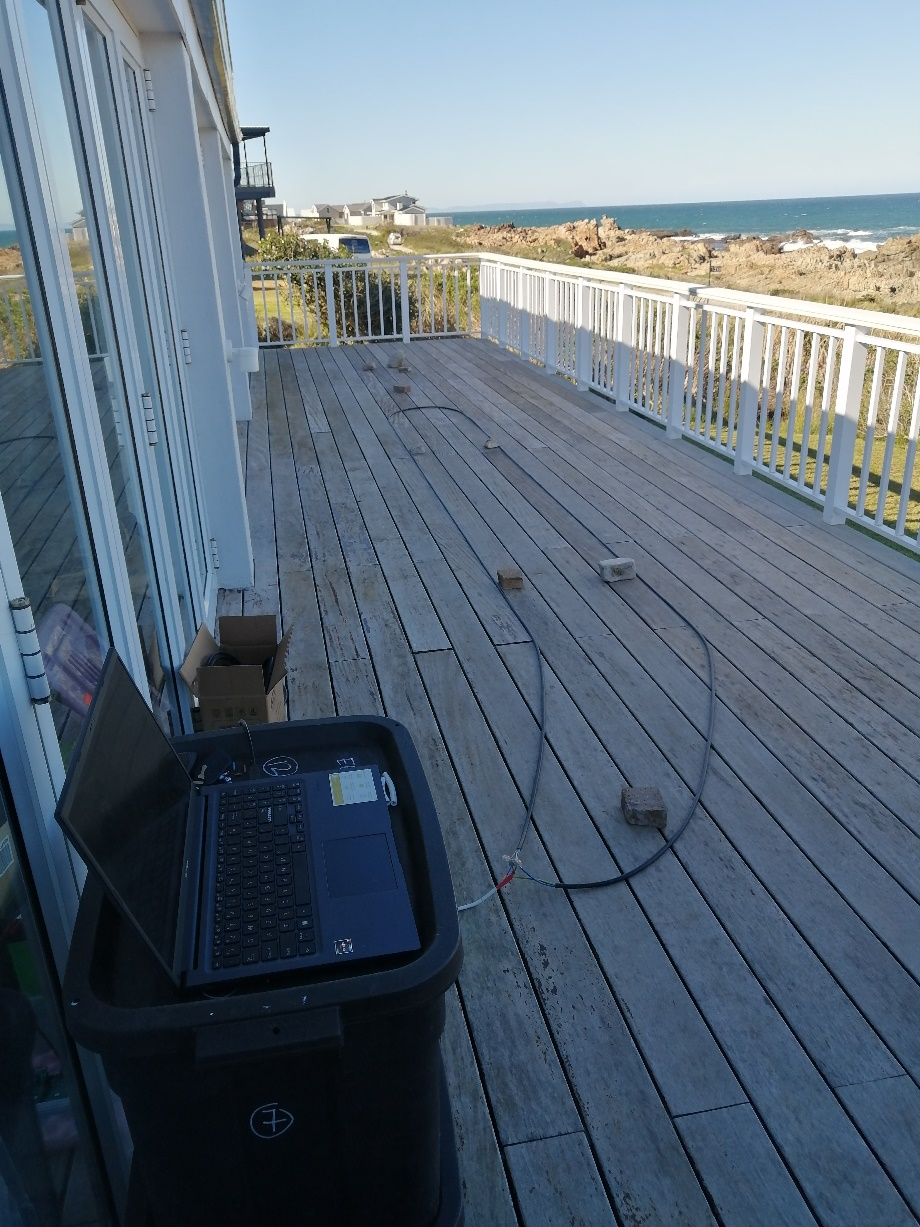
\includegraphics[width=6.25in,height=\textheight,keepaspectratio]{images/media/61_antenna.jpeg}

}

\caption{\textbf{Figure 61.} Laying out the 3-core cable to build a RFID
antenna.}

\end{figure}%

\begin{itemize}
\item
  Once the antenna is connected and you have logged into the BioMark via
  minicom (or the Device Manager software), the antenna can be tested.
  In the BioMark console, send the command ``aft''. This is ``Antenna
  Full Tune''. The reader will try to tune the antenna by adding
  capacitance and give a final ``caps'' value between 0 and 1023. As the
  antenna cable is too long at the start, the number should be low.
\item
  Cut a piece of the cable off, connect in the same fashion and test
  again. The number might remain the same until the antenna starts
  getting close to resonance.
\item
  Repeat this process until a caps value of approximately 512 is
  reached.
\item
  Be careful not to cut too much off, as the number starts growing
  rapidly once it gets close to resonance.
\item
  At this stage, the antenna current should also have increase. (above 3
  A)
\item
  Test the range of the new antenna with a test tag. Use the same test
  procedure when placing an antenna in the field.
\item
  Solder the wires and insulate using heat shrink to prevent moisture
  from corroding the joints
\end{itemize}

Note, when testing in the field, the caps number will vary wildly as the
antenna shape is changed. The important thing is that the antenna tunes,
and a tag is picked up from a decent distance. A screenshot of an
antenna tested in the field (caps = 688) can be seen in Fig. 62.

\begin{figure}[H]

{\centering 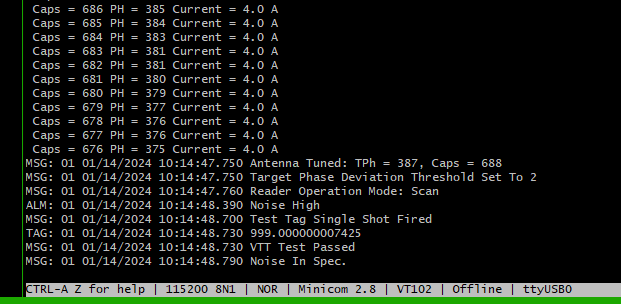
\includegraphics[width=6.25in,height=\textheight,keepaspectratio]{images/media/62_antenna.png}

}

\caption{\textbf{Figure 62.} Antenna tuning example.}

\end{figure}%

\chapter{Testing Each Script}\label{testing-each-script}

Each part of the system can now be tested individually.

\begin{itemize}
\item
  The main scripts are:

  \begin{itemize}
  \item
    scale.py
  \item
    rfid.py
  \item
    system\_status\_check.py
  \item
    transfer\_data.py
  \item
    apms\_email.py
  \item
    log.py
  \end{itemize}
\end{itemize}

\section{Testing the scales.py
script}\label{testing-the-scales.py-script}

Before testing, ensure the APMS is configured - See
\hyperref[Configuringux5cux2520theux5cux2520APMS]{Configuring the APMS}.

\begin{itemize}
\item
  Plug both scales into their respective sockets.
\item
  Power up the APMS Main Unit
\item
  SSH into the Pi.
\item
  Check if the scales service is running in the background and stop the
  service if it is:

  \begin{itemize}
  \tightlist
  \item
    Check with:
  \end{itemize}

\begin{Shaded}
\begin{Highlighting}[]
\ExtensionTok{systemctl}\NormalTok{ status scales}
\end{Highlighting}
\end{Shaded}

  \begin{itemize}
  \tightlist
  \item
    If active, stop the service:
  \end{itemize}

\begin{Shaded}
\begin{Highlighting}[]
\FunctionTok{sudo}\NormalTok{ systemctl stop scales}
\end{Highlighting}
\end{Shaded}
\item
  Ensure the indicators show weight readings of close to 0.000 kg (It
  should be within 1g after calibration)
\item
  Check the scale frequencies:
\end{itemize}

\begin{Shaded}
\begin{Highlighting}[]
\ExtensionTok{python3}\NormalTok{ \textasciitilde{}/apms/test\_scale\_frequency.py}
\end{Highlighting}
\end{Shaded}

\begin{itemize}
\item
  Currently the scales are set to 100 Hz.
\item
  Check that the scale frequencies are within 1\% (between 99 Hz and 101
  Hz)
\item
  Run the scales script:
\end{itemize}

\begin{Shaded}
\begin{Highlighting}[]
\ExtensionTok{python3}\NormalTok{ \textasciitilde{}/apms/scales.py}
\end{Highlighting}
\end{Shaded}

\begin{itemize}
\tightlist
\item
  You should see the following on the screen:
\end{itemize}

\begin{figure}[H]

{\centering 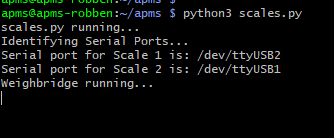
\includegraphics[width=6.25in,height=\textheight,keepaspectratio]{images/media/63_scsales_py.png}

}

\caption{\textbf{Figure 63.} A screen shot of the scale.py script
running.}

\end{figure}%

\begin{itemize}
\item
  Put a \ul{1kg} weight on \ul{scale 1}.
\item
  As it is less than the weight of a penguin, and less than the weight
  specified in the config.json file, it should detect a high dead
  weight.
\item
  Check that it is indeed \ul{scale 1} showing the high dead weight
  (Fig. 64).
\item
  Remove the \ul{1kg} weight. A message should state the dead weight has
  reduced (Fig. 64).
\item
  Repeat for scale 2
\end{itemize}

\begin{figure}[H]

{\centering 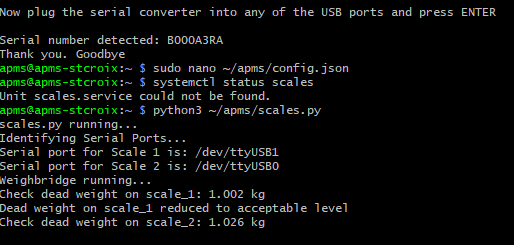
\includegraphics[width=6.25in,height=\textheight,keepaspectratio]{images/media/64_deadweight.png}

}

\caption{\textbf{Figure 64.} Dead weight message printed in the
terminal.}

\end{figure}%

\begin{itemize}
\item
  Place a \ul{5kg} weight on \ul{scale 1}.

  \begin{itemize}
  \item
    As this weight is greater than the minimum penguin weight, an event
    should be started. As scale 1 was triggered first, it should
    indicate a penguin heading out to the ocean.
  \item
    Wait a few seconds and remove the 5kg weight. After removing the
    weight, there will be a slight pause and then the event should
    finish, and the data stored to a file. This pause is the time period
    set in the config file for ``SCALE\_EMPTY\_TIME''.
  \item
    A screenshot is shown below:
  \end{itemize}
\end{itemize}

\begin{figure}[H]

{\centering 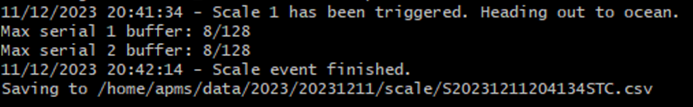
\includegraphics[width=6.25in,height=\textheight,keepaspectratio]{images/media/65_scale_event.png}

}

\caption{\textbf{Figure 65.} Example of a scale file written to file.}

\end{figure}%

\begin{itemize}
\tightlist
\item
  Repeat for \ul{scale 2}. This time, the system should detect \ul{scale
  2} being triggered first, displaying a message that a penguin is
  coming back from the ocean. Remove the weight and wait for the event
  to finish.
\end{itemize}

The testing of the scales is now complete. The files generated in the
above tests can be checked for accuracy after uploading them to the
cloud using the \texttt{transfer\_data.py} script (see section below).

\section{Testing the rfid.py script}\label{testing-the-rfid.py-script}

The APMS picks up RFID tags via an external RFID reader made by BioMark
(Model IS1001).

\begin{itemize}
\item
  Before testing the rfid script, please ensure the BioMark Reader has
  been fully configured and the BioMark antenna installed. See
  \hyperref[Configuringux5cux2520theux5cux2520BioMarkux5cux2520Reader]{Configuring
  the BioMark Reader}.
\item
  Connect a cable between the mini-USB port on the BioMark Reader and
  the front USB port of the APMS main unit.

  \begin{itemize}
  \tightlist
  \item
    If an APMS main unit is not being used, the Raspberry Pi will have
    to be powered by a 5V power supply and any USB port on the Pi can be
    used to connect to the BioMark Reader.
  \end{itemize}
\item
  Power up the BioMark Reader and APMS main unit.
\item
  SSH into the Pi.
\item
  Check that the rfid service is not running in the background and stop
  the service if it is. Check with:
\end{itemize}

\begin{Shaded}
\begin{Highlighting}[]
\ExtensionTok{systemctl}\NormalTok{ status rfid}
\end{Highlighting}
\end{Shaded}

\begin{itemize}
\tightlist
\item
  If active, stop the service:
\end{itemize}

\begin{Shaded}
\begin{Highlighting}[]
\FunctionTok{sudo}\NormalTok{ systemctl stop rfid}
\end{Highlighting}
\end{Shaded}

\begin{itemize}
\tightlist
\item
  Run the rfid script:
\end{itemize}

\begin{Shaded}
\begin{Highlighting}[]
\ExtensionTok{python3}\NormalTok{ \textasciitilde{}/apms/rfid.py}
\end{Highlighting}
\end{Shaded}

\begin{itemize}
\tightlist
\item
  You should see the following on the screen (Fig. 66). Note that the
  RFID reader could be assigned to ``\emph{ttyUSB0''},''\emph{ttyUSB1''}
  or ``\emph{ttyUSB2''}.
\end{itemize}

\begin{figure}[H]

{\centering 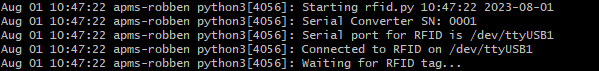
\includegraphics[width=6.25in,height=\textheight,keepaspectratio]{images/media/66_rfid_py.png}

}

\caption{\textbf{Figure 66.} Running the rfid.py script.}

\end{figure}%

\begin{itemize}
\tightlist
\item
  Take a test tag and move it close to the antenna. The tag should be
  registered and saved to a file. This file can also be checked after
  uploading to the cloud. The tag should be read and printed out (Fig.
  67).
\end{itemize}

\begin{figure}[H]

{\centering 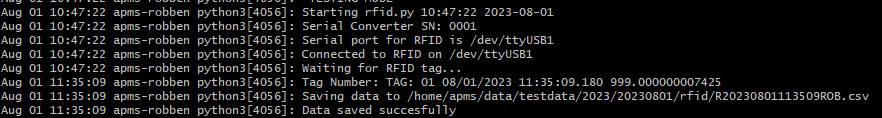
\includegraphics[width=7.29167in,height=\textheight,keepaspectratio]{images/media/67_rfid_py.png}

}

\caption{\textbf{Figure 67.} RFID tag being read by the Biomark.}

\end{figure}%

\section{Testing the system\_status\_check.py
script}\label{testing-the-system_status_check.py-script}

The \texttt{system\_status\_check.py} script automatically runs every
hour, at 10 past the hour. The script is used to monitor the health of
the entire APMS. See Fig. 68 for a screenshot after running the script
manually. The main features of the script are:

\begin{itemize}
\item
  Send an SMS to the operator if the Raspberry Pi has rebooted.
\item
  Check Last time data was uploaded and backfill data if needed.
\item
  The script will check when last the data was uploaded to the cloud and
  if more than a day, the data transfer script will be executed to
  upload all outstanding data.
\item
  Check CPU temperature
\item
  If the CPU temperature exceeds the WARNING or DANGER thresholds, an
  email will be sent to the operator. Thresholds are set in the
  configuration file. See
  \hyperref[Configuringux5cux2520theux5cux2520APMS]{Configuring the
  APMS} and adjust \texttt{CPU\_TEMP\_WARNING} and
  \texttt{CPU\_TEMP\_DANGER} variables.
\item
  Checks CPU load and memory usage
\item
  Checks USB Flash drive is mounted and storage available
\item
  Tests the internet connection
\item
  Check if a BASH command has been received from Monitor and executes it
  (still in development)
\item
  Receives status report from Arduino Monitor (Used for Dashboard)
\item
  Sends a report to the Arduino Monitor

  \begin{itemize}
  \tightlist
  \item
    Used when requesting a status report from the Monitor, via SMS.
  \end{itemize}
\end{itemize}

All the information is logged to a daily system status file. This file
will normally have 24 entries, one for every hour. On occasion, the
request for a status report from the Monitor might fail. The operator
should receive an email alert. If this happens, wait one hour and check
if the next status report is received (at 10 past the hour). If not
investigate.

The daily status file can be viewed with the \texttt{cat} function and
files are located at:

\textasciitilde/data/{[}YEAR{]}/{[}YYYYMMDD{]}/{[}YYYYMMDD{]}*\_STATUS.txt

For example:
\texttt{cat\ \textasciitilde{}/data/2023/20231230/20231230\_STATUS.txt}

This file is uploaded to the cloud daily and most of the info on the
Dashboard is obtained from this file.

To test the system\_status\_check.py script, do the following:

\begin{itemize}
\tightlist
\item
  Run the script:
\end{itemize}

\begin{Shaded}
\begin{Highlighting}[]
\ExtensionTok{python3}\NormalTok{ \textasciitilde{}/apms/system\_status\_check.py}
\end{Highlighting}
\end{Shaded}

A typical output is shown in Fig. 68.

\begin{figure}[H]

{\centering 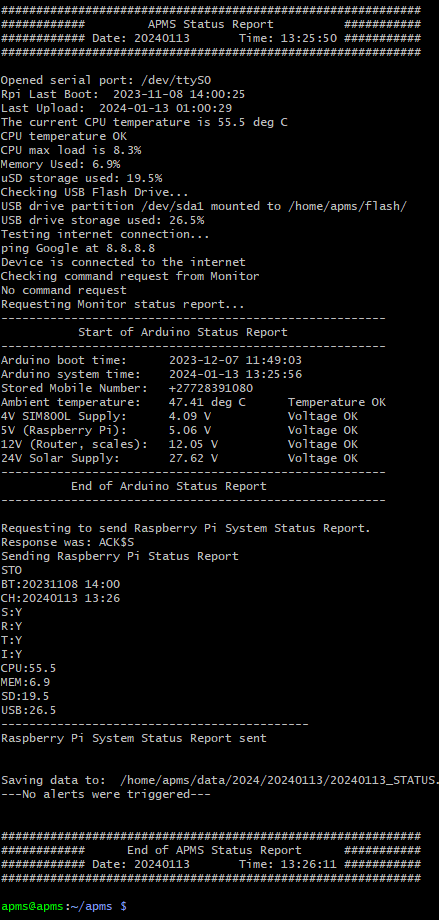
\includegraphics[width=6.25in,height=\textheight,keepaspectratio]{images/media/68_system_status.png}

}

\caption{\textbf{Figure 68.} Example of a system status report.}

\end{figure}%

\section{Testing the transfer\_data.py
script}\label{testing-the-transfer_data.py-script}

The APMS system stores data in three places. Initially, the raw files
are saved to the internal micro-SD card of the Raspberry Pi. Every
morning at 1AM the new data is transferred to the USB Flash drive and to
the cloud. This upload time can be changed in the config file
(\texttt{UPLOAD\_HOUR}) If there is no internet connection or if the
connection fails during data transfer, the \emph{last\_upload.txt} file
will not be updated. The \emph{last\_upload.txt} file (located at
\emph{\textasciitilde/logs/last\_upload.txt)} is checked by the
\texttt{system\_status\_check.py} script that runs every hour.

The APMS uses AWS S3 for cloud storage. It is the responsibility of the
administrator to manage the storage space available on the USB Flash
drive and the internal micro-SD card. Both these parameters can be
viewed on the dashboard and an alert is set for when either one reaches
75\% capacity.

\begin{itemize}
\item
  Ensure there are some data files to transfer and that the APMS has
  been configured. If you have already completed the testing of the
  \hyperref[Testingux5cux2520theux5cux2520scales.pyux5cux2520script]{scales}
  and
  \hyperref[Testingux5cux2520theux5cux2520rfid.pyux5cux2520script]{rfid}
  scripts, there should be some test files to transfer.
\item
  Run the data transfer script:
\end{itemize}

\begin{Shaded}
\begin{Highlighting}[]
\ExtensionTok{python3}\NormalTok{ \textasciitilde{}/apms/transfer\_data.py}
\end{Highlighting}
\end{Shaded}

\begin{itemize}
\tightlist
\item
  You should see something similar to the screenshot in Fig. 69.
\end{itemize}

\begin{figure}[H]

{\centering 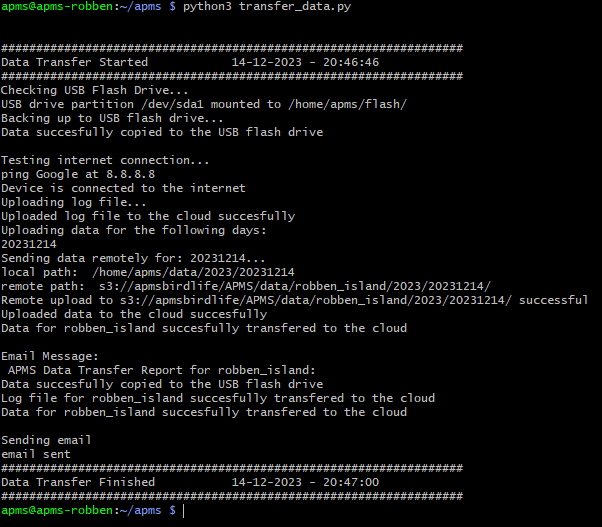
\includegraphics[width=6.25in,height=\textheight,keepaspectratio]{images/media/69_transfer_data.png}

}

\caption{\textbf{Figure 69.} Example of running the transfer\_data.py
script.}

\end{figure}%

\begin{itemize}
\item
  Every time data is successfully uploaded, the file
  \emph{\textasciitilde/logs/last\_upload.txt} is updated.
\item
  To verify today's date and time was added to the bottom of the file
  after the transfer, run:
\end{itemize}

\begin{Shaded}
\begin{Highlighting}[]
\FunctionTok{cat}\NormalTok{ \textasciitilde{}/logs/last\_upload.txt}
\end{Highlighting}
\end{Shaded}

\begin{itemize}
\item
  To check if the data transferred to the USB Flash drive:

  \begin{itemize}
  \item
    Ensure it is mounted. See
    \hyperref[Setux5cux2520upux5cux2520theux5cux2520USBux5cux2520Flashux5cux2520Drive]{Set
    up the USB Flash Drive}.
  \item
    List the files in the scale and rfid data directory. For example, to
    list the files for today, the 15\textsuperscript{th} of December
    2023. Adapt the lines below for the day the test was conducted.
  \end{itemize}
\end{itemize}

\begin{Shaded}
\begin{Highlighting}[]
\FunctionTok{ls}\NormalTok{ \textasciitilde{}/flash/2023/20231215/scale/}
\FunctionTok{ls}\NormalTok{ \textasciitilde{}/flash/2023/20231215/rfid/}
\end{Highlighting}
\end{Shaded}

\begin{itemize}
\item
  To check if the data transferred to the cloud:

  \begin{itemize}
  \item
    Open an S3 Client, such as S3 Browser.
  \item
    Check the scale and rfid data directory. For example, the scale and
    rfid directories for Stony Point, for the 15\textsuperscript{th} of
    December 2023, can be found at:

    \begin{itemize}
    \item
      \emph{s3://apmsbirdlife/APMS/data/stony\_point/2023/20231215/scale/}
    \item
      \emph{s3://apmsbirdlife/APMS/data/stony\_point/2023/20231215/rfid/}
    \end{itemize}
  \end{itemize}
\end{itemize}

\section{Testing the apms\_email.py
script}\label{testing-the-apms_email.py-script}

The apms\_email.py script is a useful script that can be run from the
command line to send an email. The script is also capable of sending a
file as an attachment. It is important to check this script is working,
as it will be used to email the operator in case of a fault.

The syntax is as follows:
\texttt{python3\ apms\_email.py\ "body\ of\ email"\ \textbackslash{}{[}path\ to\ attachment\ file\textbackslash{}{]}}

example:

\begin{Shaded}
\begin{Highlighting}[]
\ExtensionTok{python3}\NormalTok{ \textasciitilde{}/apms/apms\_email.py }\StringTok{"this is the body of the email"}\NormalTok{ \textasciitilde{}/attachment.zip}
\end{Highlighting}
\end{Shaded}

If the script was not successful, examine the email information in the
APMS configuration file. See
\hyperref[Configuringux5cux2520theux5cux2520APMS]{Configuring the APMS}

\section{Testing the log.py script}\label{testing-the-log.py-script}

The \texttt{log.py} script is crucial and should be used whenever a
calibration is done, something unusual is detected with the system, when
any structural/firmware/hardware changes are made, or when any general
work is carried out. The log script will make a backup of the existing
log file whenever a log entry is added. The backed-up log files can be
found at: \textbf{\textasciitilde/logs/backup}

To use the log script:

\begin{itemize}
\item
  SSH into the Pi.
\item
  Run the log script:
\end{itemize}

\begin{Shaded}
\begin{Highlighting}[]
\ExtensionTok{python3}\NormalTok{ \textasciitilde{}/apms/log.py}
\end{Highlighting}
\end{Shaded}

\begin{itemize}
\tightlist
\item
  Follow the onscreen commands to log an entry
\end{itemize}

If this is the first log entry, a new log file will be created
(\textasciitilde/logs/log.txt)

\begin{itemize}
\tightlist
\item
  View the log file to check the entry was added
\end{itemize}

\begin{Shaded}
\begin{Highlighting}[]
\FunctionTok{cat}\NormalTok{ \textasciitilde{}/logs/log.txt}
\end{Highlighting}
\end{Shaded}

\begin{itemize}
\tightlist
\item
  Edit the log file if a change needs to be made:
\end{itemize}

\begin{Shaded}
\begin{Highlighting}[]
\FunctionTok{sudo}\NormalTok{ nano \textasciitilde{}/logs/log.txt}
\end{Highlighting}
\end{Shaded}

The log entries are displayed on the Dashboard.

\section{Assigning an RFID Tag to a
Penguin}\label{assigning-an-rfid-tag-to-a-penguin}

After the scale file is analysed and a list of penguins is generated,
RFID tags can be assigned. For each penguin, a ``crossing time'' is
calculated. A penguin crossing is defined as the period between first
stepping on the scales until stepping off the scales. A single
``crossing time'' is calculated as halfway through the penguin crossing.

For each penguin, the crossing time is compared to the RFID timestamps
to check if an RFID tag was picked up close to when the penguin crossed
the scales (\texttt{RFID\_TO\_PENGUIN\_INTERVAL} in the config file). By
default, \texttt{RFID\_TO\_PENGUIN\_INTERVAL} is set to 60 seconds.

The location of the RFID antenna is set in the config file for each
site. Look for
\texttt{\textquotesingle{}RFID\_LOCATION\textquotesingle{}:\ \textquotesingle{}MIDDLE\_ONLY\textquotesingle{}}
near the bottom of \texttt{config.py}. The default is
\texttt{\textquotesingle{}MIDDLE\_ONLY\textquotesingle{}}, as this is
the configuration for all new sites. This is not the case for older
sites (see later in this chapter).

When \texttt{\textquotesingle{}MIDDLE\_ONLY\textquotesingle{}} is given
as the RFID antenna location, and no other RFID tags were recorded
during the penguin's crossing, the algorithm can assign an RFID tag
number to the penguin based on the following two scenarios:

\begin{enumerate}
\def\labelenumi{\arabic{enumi}.}
\tightlist
\item
  \textbf{The tag is picked up during the jump from one scale to the
  other:} If a tag is picked up within the time period when the penguin
  is jumping from one scale to the other, the tag number is assigned to
  that penguin. This is also valid for a group of penguins, as we assume
  they move in single file over the scales. This is why it is important
  to ensure they move in single file when setting up the site: to avoid
  a penguin overtaking another and causing the event to be discarded or,
  worse, an incorrect RFID tag assigned to a penguin.
\item
  \textbf{The tag was picked up somewhere during the penguin's crossing
  (no other penguins crossing):} Sometimes, due to various
  circumstances, the antenna will pick up the tag too early, or even
  after the jump. If, however, we know the antenna is placed in between
  the scales, and no other penguins were crossing at the same time, we
  assume the tag belongs to that penguin.
\end{enumerate}

Below is an example of two penguins heading out to the ocean. They each
trigger the BioMark RFID reader as they jump from Scale 1 (colony side)
to Scale 2 (ocean side), and thus both have RFID tag numbers assigned to
them.

As a final ``basic check'', the algorithm checks for the following
parameters set in the config file:

\begin{itemize}
\tightlist
\item
  The tag was picked up close to when a penguin was crossing
  (\texttt{RFID\_TO\_PENGUIN\_INTERVAL}, default: 60 sec)\\
\item
  \textbf{AND} the tag was the only one for a certain period of time
  (\texttt{RFID\_ISOLATION\_INTERVAL}, default: 5 minutes)\\
\item
  \textbf{AND} it was the only scale file generated for a certain period
  of time (\texttt{SCALE\_FILE\_ISOLATION\_INTERVAL}, default: 60
  seconds)\\
\item
  \textbf{AND} there was only one penguin in the above-mentioned scale
  file.
\end{itemize}

\section{Error Handling}\label{error-handling}

Penguins are wild animals and do not always walk nicely over the scales.
Numerous situations can give rise to a scale file not being processed. A
fault with the scale could also lead to data files that cannot be
processed by the algorithm.

When the algorithm discards a file, it moves it to an ``error''
directory with the name of the error. These files can then be viewed
separately to learn more. The error directories are located in the
``processed'' folder at:

\texttt{\textasciitilde{}\textbackslash{}APMS\_DATA\_PROCESSING\textbackslash{}DATA\textbackslash{}PROCESSED\textbackslash{}{[}SITE\ NAME{]}\textbackslash{}{[}YEAR{]}\textbackslash{}{[}YYYYMMDD{]}\textbackslash{}{[}ERROR\ DIRECTORY{]}}

Note that even though these are called ``error'' directories, it does
not mean there is a hardware fault. For instance, if another animal
triggers the scale, the algorithm detects that and moves it to the
\texttt{NO\_PENGUINS} error directory. Many of these errors are
triggered based on parameters set in the config file.

When a site is not performing as expected, viewing these directories can
often give clues as to what is wrong.

This system can be expanded, with different error states added as
required. (Adding a visualization of this to the APMS Dashboard is a
recommended future addition.)

\subsection{Error Directory Reference}\label{error-directory-reference}

\begin{longtable}[]{@{}
  >{\raggedright\arraybackslash}p{(\linewidth - 2\tabcolsep) * \real{0.5000}}
  >{\raggedright\arraybackslash}p{(\linewidth - 2\tabcolsep) * \real{0.5000}}@{}}
\toprule\noalign{}
\begin{minipage}[b]{\linewidth}\raggedright
Error Directory
\end{minipage} & \begin{minipage}[b]{\linewidth}\raggedright
Reason
\end{minipage} \\
\midrule\noalign{}
\endhead
\bottomrule\noalign{}
\endlastfoot
\texttt{TIMING\_JUMP} & Large time difference between samples in scale
file (\textgreater{} 1 second). \\
\texttt{FREQUENCY\_ERROR} & Scale sampling period is not correct.
Configured via \texttt{MAX\_AVG\_SAMPLING\_PERIOD} and
\texttt{MIN\_AVG\_SAMPLING\_PERIOD}. \\
\texttt{NO\_SUB\_EVENTS} & No sub-events found in scale file. \\
\texttt{UNEQUAL\_NUM\_PENGUINS} & Number of penguins determined for
Scale 1 differs from Scale 2. \\
\texttt{NO\_PENGUINS} & List of penguins for Scale 1 and Scale 2 are
both empty. \\
\texttt{DIRECTION\_ERROR} & Different number of penguins going out to
the ocean than coming back. \\
\texttt{PENGUIN\_WEIGHT\_ERROR} & Algorithm could not determine a weight
from the provided data. \\
\texttt{WEIGHT\_TOO\_HIGH} & Weight was recorded as \textgreater{} 3x
max penguin weight. Configured via \texttt{MAX\_PENGUIN\_WEIGHT}. \\
\texttt{OVERLOAD} & Weight exceeded scale maximum. Configured via
\texttt{SCALE\_OVERLOAD}. \\
\texttt{DUPLICATE\_TIMESTAMPS} & Weights with the exact same timestamp
found in scale file. \\
\texttt{LARGE\_PENGUIN\_WEIGHT\_DIFFERENCE} & Large difference in weight
between Scale 1 and Scale 2. Configured via
\texttt{MAX\_SCALES\_DIFFERENCE\_ALLOWED}. \\
\texttt{NO\_DEAD\_WEIGHT\_EVENTS} & No periods found where the scale was
reading a stationary dead weight. \\
\texttt{LARGE\_DEAD\_WEIGHT} & Weight on empty scale before/after event
is higher than allowed. Configured via \texttt{MAX\_DEAD\_WEIGHT}. \\
\texttt{LARGE\_DEAD\_WEIGHT\_DIFFERENCE} & Difference between dead
weight before hopping on vs.~after hopping off is too large. Configured
via \texttt{MAX\_DEADWEIGHT\_DIFF}. \\
\texttt{NEGATIVE\_JUMP\_TIME} & Calculation of time taken to jump
between scales returned a negative result. \\
\texttt{NEGATIVE\_TIME\_ON\_SCALE} & Calculated time of jumping onto
scale occurs \emph{after} jumping off scale. \\
\end{longtable}

\section{Testing the ON/OFF Button}\label{testing-the-onoff-button}

Ensure the system is ready to be powered down before starting this test.
Stop the rfid and scale services.

To test the ON/OFF button, simply press it. The Raspberry Pi should
start shutting down if it was on. The lights will flash and eventually a
solid red light will be seen. If the Raspberry Pi was off, it should
boot up.

If it does not work, check the wiring of the button on the Monitor, as
well as the configuration of GPIO on the Pi. See
\hyperref[Configureux5cux2520GPIO3ux5cux2520forux5cux2520Powerux5cux2520ONux2fOFF]{Configure
GPIO3 for Power ON/OFF} for more info. Another way to isolate the fault
is to power down the Pi via the Monitor command: \texttt{CMD:P}. If this
works, the Pi has been configured properly and the problem lies
elsewhere.

\section{Testing the update\_system\_time.py
script}\label{testing-the-update_system_time.py-script}

To prevent the system clock updating at random times, the updating of
the system clock is handled by the update\_system\_time.py script. This
is to prevent the clock updating while penguins are crossing. Causing
timing errors. Files with timing errors will be rejected by the data
processing algorithm, so to reduce the chance of this happening, a
better time for updating the clock is chosen

This script runs every Monday, at 12:00. This is set in the crontab
(see: \hyperref[Configureux5cux2520theux5cux2520Crontab]{Configure the
Crontab}). The script checks that no penguins cross the scales for 10
minutes and then updates the time. Even though this is not foolproof, it
provides a safer moment in time to update the clock.

To test, run the \texttt{update\_system\_time.py} script:

\begin{Shaded}
\begin{Highlighting}[]
\FunctionTok{sudo}\NormalTok{ python3 \textasciitilde{}/apms/update\_system\_time.py}
\end{Highlighting}
\end{Shaded}

The script will run, wait for 10 minutes, and update the system time.

To view previous times when the clock was updated, view the log file at:
\texttt{\textasciitilde{}/logs/update\_time.log}

\section{Configure Scripts as
Services}\label{configure-scripts-as-services}

For a new system, the rfid and scales scripts need to be configured to
run in the background, as processes.

There are 2 main service files: scales.service and rfid.service. The
service files are located at \texttt{\textasciitilde{}/apms/services/}.
To perform these operations, ensure you SSH in locally, not via
Tailscale.

Copy the 2 service files to the appropriate directory:

\begin{Shaded}
\begin{Highlighting}[]
\FunctionTok{sudo}\NormalTok{ cp \textasciitilde{}/apms/services/}\PreprocessorTok{*}\NormalTok{.service /etc/systemd/system/}
\end{Highlighting}
\end{Shaded}

Start and enable each service:

\begin{Shaded}
\begin{Highlighting}[]
\ExtensionTok{systemctl}\NormalTok{ start scales}
\ExtensionTok{systemctl}\NormalTok{ enable scales}
\ExtensionTok{systemctl}\NormalTok{ start rfid}
\ExtensionTok{systemctl}\NormalTok{ enable rfid}
\end{Highlighting}
\end{Shaded}

Check that the services are active by running:

\begin{Shaded}
\begin{Highlighting}[]
\ExtensionTok{systemctl}\NormalTok{ status scales}
\ExtensionTok{systemctl}\NormalTok{ status rfid}
\end{Highlighting}
\end{Shaded}

Reboot the Pi:

\begin{Shaded}
\begin{Highlighting}[]
\FunctionTok{sudo}\NormalTok{ reboot}
\end{Highlighting}
\end{Shaded}

Wait a minute and try to SSH in remotely (via the internet). If this
works, you have successfully configured tmate as a service. SSH into the
Pi, either locally or via tmate and check that the scales and rfid
services are running.

\begin{Shaded}
\begin{Highlighting}[]
\ExtensionTok{systemctl}\NormalTok{ status scales}
\ExtensionTok{systemctl}\NormalTok{ status rfid}
\end{Highlighting}
\end{Shaded}

\chapter{Configure the Crontab}\label{configure-the-crontab}

The crontab is a task scheduler and is responsible for the following:

\begin{itemize}
\item
  Check the system every hour.
\item
  Transfer APMS data to the cloud every day.
\item
  Update the system clock once a week, and at boot.
\end{itemize}

The crontab sends the output of each script to a log file. See
\texttt{\textasciitilde{}/logs/}

\section{Setting up the Crontab}\label{setting-up-the-crontab}

To configure the crontab:

\begin{itemize}
\tightlist
\item
  Run:
\end{itemize}

\begin{Shaded}
\begin{Highlighting}[]
\FunctionTok{crontab} \AttributeTok{{-}e}
\end{Highlighting}
\end{Shaded}

\begin{itemize}
\item
  If a message comes up asking to choose a text editor, choose
  \texttt{nano}.
\item
  Copy and paste the following into the text editor, at the bottom of
  the file. See Fig. 70 as an example.
\end{itemize}

\begin{Shaded}
\begin{Highlighting}[]
\ExtensionTok{10} \PreprocessorTok{*} \PreprocessorTok{*} \PreprocessorTok{*} \PreprocessorTok{*}\NormalTok{ /usr/bin/python3 /home/apms/apms/system\_status\_check.py }\OperatorTok{\textgreater{}\textgreater{}}\NormalTok{ /home/apms/logs/system\_status\_check.log }\DecValTok{2}\OperatorTok{\textgreater{}\&}\DecValTok{1}
\ExtensionTok{0}\NormalTok{ 1 }\PreprocessorTok{*} \PreprocessorTok{*} \PreprocessorTok{*}\NormalTok{ /usr/bin/python3 /home/apms/apms/transfer\_data.py }\OperatorTok{\textgreater{}\textgreater{}}\NormalTok{ /home/apms/logs/transfer\_data.log }\DecValTok{2}\OperatorTok{\textgreater{}\&}\DecValTok{1}
\ExtensionTok{0}\NormalTok{ 12 }\PreprocessorTok{*} \PreprocessorTok{*}\NormalTok{ 1 /usr/bin/python3 /home/apms/apms/update\_system\_time.py }\OperatorTok{\textgreater{}\textgreater{}}\NormalTok{ /home/apms/logs/update\_time.log }\DecValTok{2}\OperatorTok{\textgreater{}\&}\DecValTok{1}
\ExtensionTok{@reboot}\NormalTok{ /usr/bin/python3 /home/apms/apms/system\_status\_check.py boot }\OperatorTok{\textgreater{}\textgreater{}}\NormalTok{ /home/apms/logs/system\_status\_check.log }\DecValTok{2}\OperatorTok{\textgreater{}\&}\DecValTok{1}
\end{Highlighting}
\end{Shaded}

\begin{figure}[H]

{\centering 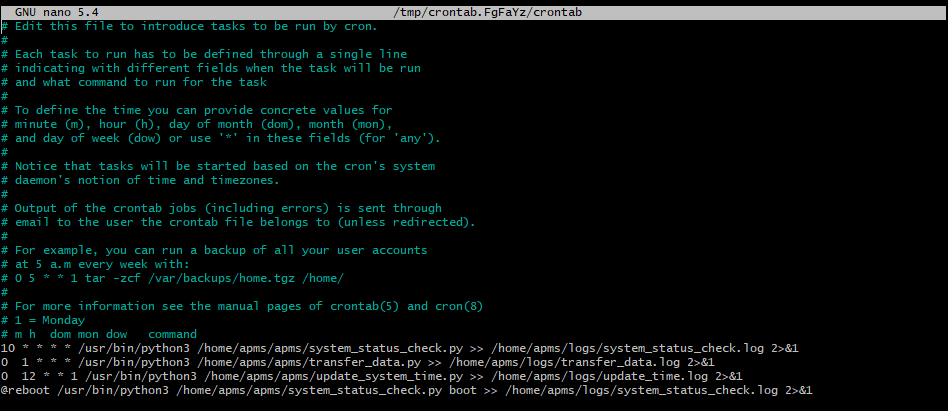
\includegraphics[width=6.25in,height=\textheight,keepaspectratio]{images/media/70_crontab.png}

}

\caption{\textbf{Figure 70.} Configuring the crontab.}

\end{figure}%

\begin{itemize}
\item
  Save and exit. (Hold \textbf{CTRL} and press \textbf{x} - Then press
  \textbf{y} to save - then press \textbf{Enter} to exit)
\item
  A message should state that the crontab has been successfully updated
  (Fig. 71).
\end{itemize}

\begin{figure}[H]

{\centering 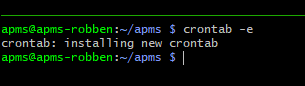
\includegraphics[width=6.25in,height=\textheight,keepaspectratio]{images/media/71_crontab.png}

}

\caption{\textbf{Figure 71} Successfully updating the crontab.}

\end{figure}%

\section{Testing the Crontab}\label{testing-the-crontab}

To test whether the crontab is working correctly, view the log files of
the scripts:

\begin{Shaded}
\begin{Highlighting}[]
\FunctionTok{cat}\NormalTok{ \textasciitilde{}/logs/system\_status\_check.log}
\FunctionTok{cat}\NormalTok{ \textasciitilde{}/logs/transfer\_data.log}
\FunctionTok{cat}\NormalTok{ \textasciitilde{}/logs/update\_time.log}
\end{Highlighting}
\end{Shaded}

\part{Deployment \& Operation}

\chapter{Commissioning a New System in the
Field}\label{commissioning-a-new-system-in-the-field}

At this stage, it is assumed that a 24V solar power supply is available
and that the entire system (Main Unit, Monitor, Scales, and BioMark RFID
reader) has been assembled and bench-tested. This section describes what
to evaluate when choosing a new field site and how to house all the
electronics.

\section{APMS Location}\label{apms-location}

When selecting an installation site for the APMS, ensure the following:

\begin{itemize}
\tightlist
\item
  \textbf{High Traffic:} Choose a path with a high rate of penguins
  crossing both to and from the ocean.
\item
  \textbf{Cable Length (Scales to Main Unit):} Keep distance manageable.
  A 10m extension cable has been field-tested and works reliably.
\item
  \textbf{Power Distance:} Account for the cable run between the 24V
  solar power supply and the Main Unit.
\item
  \textbf{Cellular Signal:} Verify strong 4G/LTE coverage at the exact
  location where the 4G router and APMS Monitor will operate (test via
  \href{https://www.speedtest.net}{Speedtest.net}).
\item
  \textbf{Camouflage \& Low Disturbance:} Minimize disturbance to the
  surrounding area. Penguins are sensitive to environmental changes and
  may bypass the weighbridge if a path looks unfamiliar. Ensure every
  inch of the scales platform is covered in dark green canvas to blend
  into the habitat.
\end{itemize}

\section{APMS Enclosure}\label{apms-enclosure}

Different site conditions require different housing strategies:

\begin{itemize}
\tightlist
\item
  \textbf{Stony Point:} Housed in a large steel box alongside the
  BioMark RFID reader.
\item
  \textbf{Dassen Island, Dyer Island \& Robben Island:} Uses a rugged
  125L Skitch box. This provides enough interior volume for the APMS
  Main Unit, BioMark circuit board, and 4G indoor router.

  \begin{itemize}
  \tightlist
  \item
    Drill entry holes for scale cables, the RFID antenna cable, and
    power lines.
  \item
    Pass cables through grommets or feed irrigation piping directly into
    the box.
  \item
    Seal cable entry points with silicone to prevent water ingress.
  \item
    Where possible, angle entry pipes slightly \textbf{upward} into the
    box so water cannot run down the exterior pipe into the enclosure.
  \end{itemize}
\item
  \textbf{Bird Island:} Uses a smaller Skitch box with the BioMark
  reader housed in a separate enclosure.
\end{itemize}

\begin{tcolorbox}[enhanced jigsaw, left=2mm, toptitle=1mm, breakable, opacitybacktitle=0.6, title=\textcolor{quarto-callout-tip-color}{\faLightbulb}\hspace{0.5em}{Enclosure Heat \& Mounting}, colback=white, opacityback=0, rightrule=.15mm, leftrule=.75mm, colbacktitle=quarto-callout-tip-color!10!white, bottomtitle=1mm, titlerule=0mm, coltitle=black, colframe=quarto-callout-tip-color-frame, arc=.35mm, bottomrule=.15mm, toprule=.15mm]

Paint the exterior of plastic enclosures white to reflect solar
radiation and lower internal temperatures. In high-wind locations (such
as Bird Island), bolt the enclosure down securely to a solid base.

\end{tcolorbox}

\begin{figure}[H]

{\centering 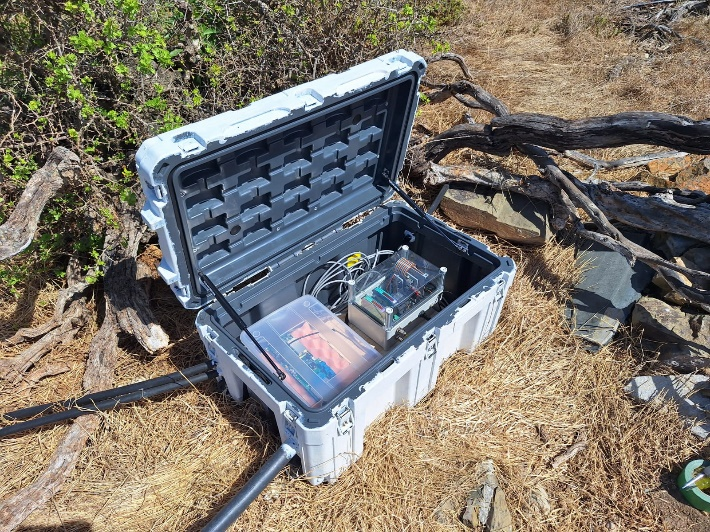
\includegraphics[width=6.25in,height=\textheight,keepaspectratio]{images/media/72_skitch.jpeg}

}

\caption{\textbf{Figure 72.} Skitch Box Enclosure Setup}

\end{figure}%

\begin{figure}[H]

{\centering 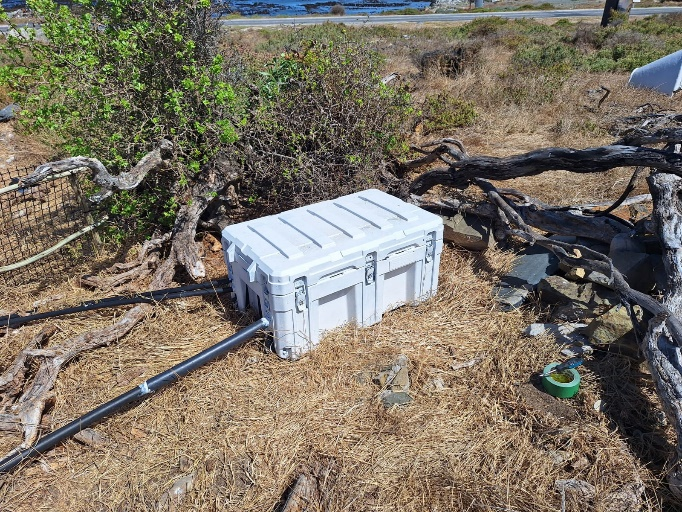
\includegraphics[width=6.25in,height=\textheight,keepaspectratio]{images/media/73_skitch.jpeg}

}

\caption{\textbf{Figure 73.} Closed Skitch Box with Irrigation Pipe
Entries}

\end{figure}%

\section{Wiring the Skitch Box}\label{wiring-the-skitch-box}

Once the box is positioned and irrigation entry pipes/grommets are
installed, begin internal wiring:

\begin{enumerate}
\def\labelenumi{\arabic{enumi}.}
\tightlist
\item
  \textbf{Power Feed:} Pass the 24V DC power wires from the solar supply
  through the irrigation pipe into the box. Split this feed to power
  both the APMS Main Unit and the BioMark Reader.
\item
  \textbf{Main Unit Power:} Solder a DC plug (\texttt{RS:\ 705-1519})
  onto the incoming 24V power line and plug it into the Main Unit.
\item
  \textbf{BioMark Power:} Wire the BioMark reader through an inline
  circuit breaker, which also serves as a manual power switch.
\item
  \textbf{Router Power:} If using an indoor router, plug it into the 12V
  DC OUT socket. If using the Teltonika router, wire it to the 24V
  supply. Always check the power requirements of any device you install.
\item
  \textbf{RFID Antenna:} Feed the BioMark antenna cable into the box and
  connect it to the terminal block on the BioMark board.
\item
  \textbf{Data Link:} Connect a mini-USB cable (\texttt{RS:\ 822-3226})
  from the mini-USB port on the BioMark reader to a USB-A port on the
  front of the Main Unit.
\end{enumerate}

\section{Installing the Scales
Platform}\label{installing-the-scales-platform}

\begin{enumerate}
\def\labelenumi{\arabic{enumi}.}
\tightlist
\item
  \textbf{Leveling:} The scales platform must be level. Use a spirit
  level across both dimensions of the frame. Use surrounding sand and
  rocks to create a flat, stable foundation.
\item
  \textbf{Cable Protection:} Run all scale cables inside irrigation
  piping back to the enclosure to protect them from weather and animal
  damage (especially where cable splices exist).
\item
  \textbf{Free Pan Movement:} Ensure the canvas-covered scale pans rest
  cleanly on their load cells without touching surrounding rocks, twigs,
  or vegetation. Contact with external objects will distort weight
  measurements.
\end{enumerate}

\begin{figure}[H]

{\centering 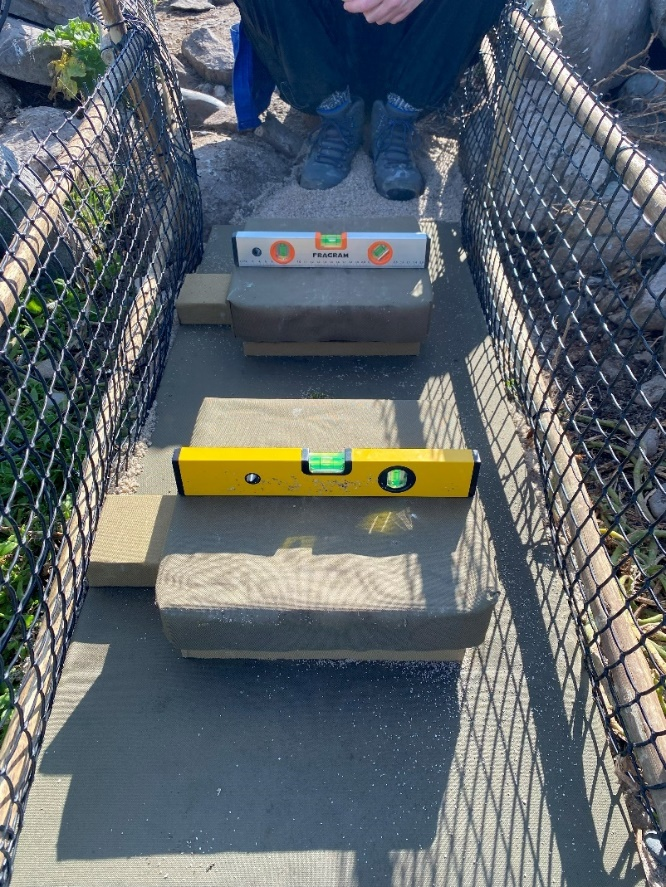
\includegraphics[width=6.25in,height=\textheight,keepaspectratio]{images/media/74_level_scales.jpeg}

}

\caption{\textbf{Figure 74.} Leveling the Scales Platform}

\end{figure}%

\begin{enumerate}
\def\labelenumi{\arabic{enumi}.}
\setcounter{enumi}{3}
\tightlist
\item
  \textbf{Antenna Placement \& Tuning:} Lay out the BioMark RFID antenna
  loop. Avoid running the antenna wire parallel to power cables, and
  never let the antenna wire overlap itself. Perform a full frequency
  tune on the BioMark reader and verify detection distance using a test
  PIT tag.
\end{enumerate}

\begin{figure}[H]

{\centering 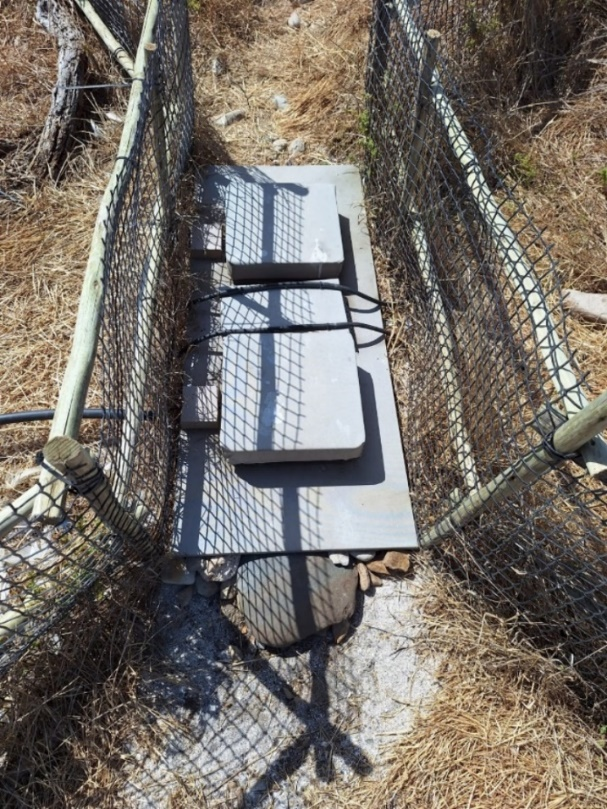
\includegraphics[width=6.25in,height=\textheight,keepaspectratio]{images/media/75_scales_antenna.jpeg}

}

\caption{\textbf{Figure 75.} RFID Antenna Layout and Tuning}

\end{figure}%

\begin{enumerate}
\def\labelenumi{\arabic{enumi}.}
\setcounter{enumi}{4}
\tightlist
\item
  \textbf{Calibration:} Once the platform is level and the RFID antenna
  is verified, calibrate the scales following the instructions in the
  section:
  \hyperref[Routineux5cux2520Calibrationux5cux2520ofux5cux2520Scales]{Routine
  Calibration of Scales}.
\end{enumerate}

\section{Warning Sign Installation}\label{warning-sign-installation}

A warning sign alerts visitors and field staff to keep clear of the
sensitive monitoring equipment.

\begin{tcolorbox}[enhanced jigsaw, left=2mm, toptitle=1mm, breakable, opacitybacktitle=0.6, title=\textcolor{quarto-callout-warning-color}{\faExclamationTriangle}\hspace{0.5em}{Security Consideration}, colback=white, opacityback=0, rightrule=.15mm, leftrule=.75mm, colbacktitle=quarto-callout-warning-color!10!white, bottomtitle=1mm, titlerule=0mm, coltitle=black, colframe=quarto-callout-warning-color-frame, arc=.35mm, bottomrule=.15mm, toprule=.15mm]

While a sign deters accidental disruption, it can also draw unwanted
attention to equipment in publicly accessible areas. The decision to
erect a sign depends on local site security.

\end{tcolorbox}

\begin{itemize}
\tightlist
\item
  \textbf{Sign Graphics File Location:}
  \texttt{{[}TODO:\ Insert\ file\ path{]}}
\item
  \textbf{Supplier Information:}
  \texttt{{[}TODO:\ Insert\ supplier\ info{]}}
\end{itemize}

\begin{figure}[H]

{\centering 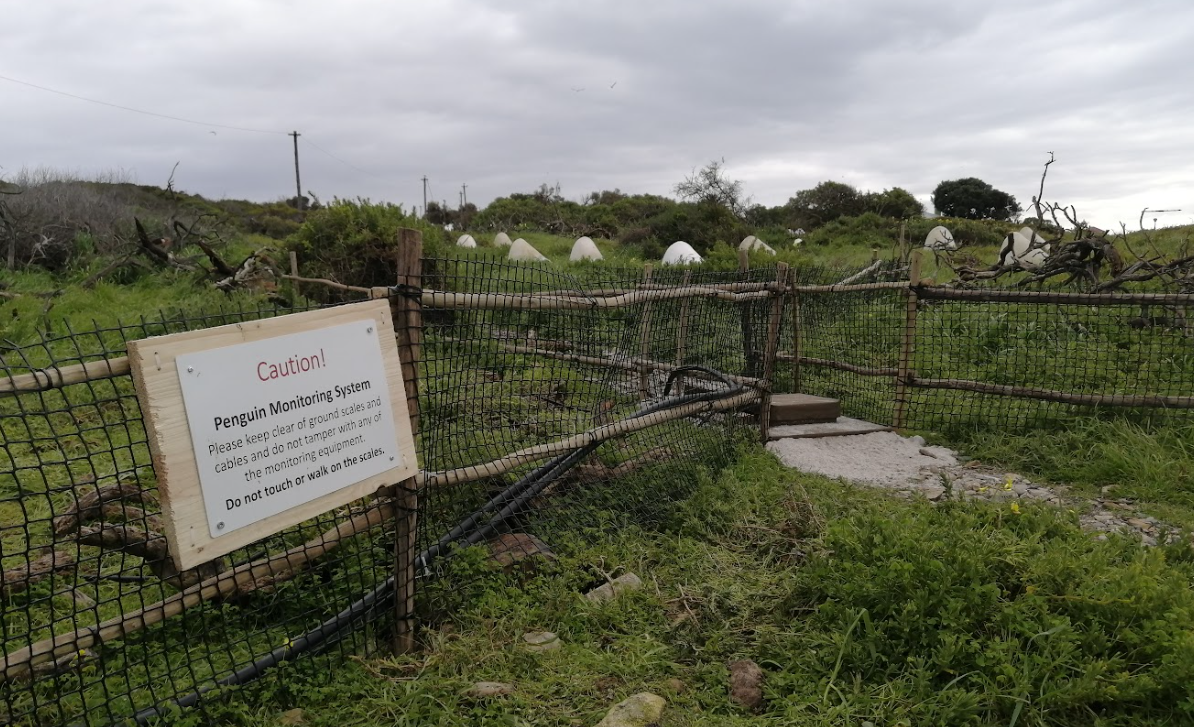
\includegraphics[width=6.25in,height=\textheight,keepaspectratio]{images/media/76_sign.png}

}

\caption{\textbf{Figure 76.} Site Warning Sign Installation}

\end{figure}%

\section{Final Checks and System
Startup}\label{final-checks-and-system-startup}

Before powering on, verify the following pre-flight checklist:

\begin{itemize}
\tightlist
\item[$\square$]
  Solar power supply outputting stable 24V DC.
\item[$\square$]
  All enclosures securely closed and latched (BioMark, APMS Main Unit,
  Router, Skitch Box).
\item[$\square$]
  BioMark reader fully wired, configured, and seated in its final
  position.
\item[$\square$]
  BioMark antenna zip-tied to mount, tuned, and field-tested with a PIT
  tag.
\item[$\square$]
  Arduino Monitor active and SIM800L antenna oriented in final position.
\item[$\square$]
  Router online with active cellular connection.
\item[$\square$]
  Field site cleared of all metal tools, loose wire, and debris.
\item[$\square$]
  Warning sign secured (if applicable).
\end{itemize}

\subsection{System Startup Sequence}\label{system-startup-sequence}

To start the system cleanly, perform a full reboot to ensure all
background scripts launch via \texttt{crontab} and \texttt{systemd}:

\begin{enumerate}
\def\labelenumi{\arabic{enumi}.}
\tightlist
\item
  Establish an SSH connection to the Main Unit (locally via LAN or
  remotely via \texttt{Tailscale}).
\item
  Issue a system reboot:
\end{enumerate}

\begin{Shaded}
\begin{Highlighting}[]
\FunctionTok{sudo}\NormalTok{ reboot}
\end{Highlighting}
\end{Shaded}

\begin{enumerate}
\def\labelenumi{\arabic{enumi}.}
\setcounter{enumi}{2}
\tightlist
\item
  Wait a few minutes and ssh into the system via \texttt{Tailscale}.
\item
  Use the tmux commands to create windows to monitor the rfid and scales
  script
\end{enumerate}

Example:

\begin{itemize}
\item
  Hold \textbf{CTRL} and press \textbf{b} - Then release keys - Then
  press \textbf{\%} to split screen vertically
\item
  Hold \textbf{CTRL} and press \textbf{b} - Then release keys - Then
  press \textbf{``} to split screen horizontally
\item
  Write the first entry into the log to state system is live:
\end{itemize}

\begin{Shaded}
\begin{Highlighting}[]
\ExtensionTok{python3}\NormalTok{ \textasciitilde{}/apms/log.py}
\end{Highlighting}
\end{Shaded}

\chapter{APMS Data Processing}\label{apms-data-processing}

The data processing section consists of the data processing script, the
code necessary to display the data on the Dashboard and a script to
generate graphs for a website. Instructions below are given for Linux,
but the data\_processing.py script can also be run on Windows.

\section{Overview}\label{overview-5}

The data processing script has the task of taking in raw scale and RFID
data and producing a csv file containing a list of penguins. The script
can be used to process multiple days over any given date range. For the
example below, only one day's data from one site is discussed. This
process is repeated for all the days of all the sites requested.

\section{Install Python Packages}\label{install-python-packages}

Install the latest version of Python if it is not installed already

\begin{Shaded}
\begin{Highlighting}[]
\ExtensionTok{pip}\NormalTok{ install matplotlib}
\ExtensionTok{pip}\NormalTok{ install pandas}
\ExtensionTok{pip}\NormalTok{ install boto3}
\ExtensionTok{pip}\NormalTok{ install scipy}
\end{Highlighting}
\end{Shaded}

\section{Download the Software from
GitHub}\label{download-the-software-from-github}

To process and display the penguin data, download the code from
\href{https://www.github.com/apmsbirdlife}{GitHub}.

\begin{itemize}
\tightlist
\item
  See the section
  \hyperref[Configureux5cux2520Gitux5cux2520andux5cux2520Downloadux5cux2520Firmware]{Configure
  Git and Download Firmware} to authenticate. Clone the directory from
  GitHub into the \texttt{home} folder. This will automatically create a
  directory called \texttt{apms\_data\_processing}.
\end{itemize}

Run the following code to clone and download the software:

\begin{Shaded}
\begin{Highlighting}[]
\BuiltInTok{cd}\NormalTok{ \textasciitilde{}}
\FunctionTok{git}\NormalTok{ clone git@github.com:apmsbirdlife/apms\_data\_processing.git}
\end{Highlighting}
\end{Shaded}

\section{Editing the config file}\label{editing-the-config-file}

All the main parameters for data processing and the Dashboard must be
set in the config file. An example file is included, called
``config\_example.py''. Edit this file and change the parameters as
required. Many of the settings can be left with their default values.
Rename the newly edited ``config\_example.py'' file to
\texttt{config.py} when you are done. Ensure this file is stored in
\textasciitilde/apms\_data\_processing, together with all the rest of
the code.

\section{Data Processing Script
Usage}\label{data-processing-script-usage}

To use the script, it is assumed that you have:

\begin{itemize}
\item
  Set up access to the cloud, as described in
  \hyperref[AWSux5cux2520S3ux5cux2520Cloudux5cux2520Storage]{AWS S3
  Cloud Storage}
\item
  Configured the config.py file as described in
  \hyperref[Editingux5cux2520theux5cux2520configux5cux2520file]{Editing
  the config file}
\end{itemize}

To process data using the script, use the following syntax:

\begin{Shaded}
\begin{Highlighting}[]
\ExtensionTok{python3}\NormalTok{ process\_data.py SITE DATE RANGE}
\end{Highlighting}
\end{Shaded}

where:

\begin{itemize}
\item
  {[}SITE{]} can be left blank to process data for all sites, or a site
  name can be given.

  \begin{itemize}
  \item
    The following site names can currently be used:

    \begin{itemize}
    \item
      ``stony\_point''
    \item
      ``bird\_island''
    \item
      ``dyer\_island''
    \item
      ``robben\_island''
    \item
      ``dassen\_island''
    \end{itemize}
  \end{itemize}
\item
  {[}DATE RANGE{]} can either be left blank, or a date range such as
  ``20230601-20231101'' can be given, or the number of days back,
  e.g.~``5''. If left blank, it will process only the previous day's
  data.
\end{itemize}

Some examples

\emph{Process the last 7 days' worth of data for Stony Point:}

\begin{Shaded}
\begin{Highlighting}[]
\ExtensionTok{python3}\NormalTok{ process\_data.py stony\_point 7}
\end{Highlighting}
\end{Shaded}

\emph{Process yesterday's data for Bird Island:}

\begin{Shaded}
\begin{Highlighting}[]
\ExtensionTok{python3}\NormalTok{ process\_data.py bird\_island}
\end{Highlighting}
\end{Shaded}

\emph{Process yesterday's data for all the sites:}

\begin{Shaded}
\begin{Highlighting}[]
\ExtensionTok{python3}\NormalTok{ process\_data.py}
\end{Highlighting}
\end{Shaded}

\emph{Process data from the first of September 2023 till the first of
November 2023, for Dyer Island:}

\begin{Shaded}
\begin{Highlighting}[]
\ExtensionTok{python3}\NormalTok{ process\_data.py dyer\_island 20230901{-}20231101}
\end{Highlighting}
\end{Shaded}

This will create a CSV file for each day. The CSV file will be stored in
the ``processed'' directory. An example of a CSV file and where it is
stored, is shown below in the following directory path:

\textasciitilde/apms\_data\_processing/data/processed/stony\_point/2023/20231227/stony\_point\_20231227\_processed\_data.csv

\section{How the Script Works}\label{how-the-script-works}

Below are the basic steps for the script to process penguin data for the
previous day.

\begin{enumerate}
\def\labelenumi{\arabic{enumi}.}
\item
  Download the previous day's scale and RFID data from the cloud (Amazon
  S3).

  \begin{enumerate}
  \def\labelenumii{\alph{enumii}.}
  \tightlist
  \item
    This gets stored in
    \textasciitilde/apms\_data\_processing/data\textbf{/downloaded\_raw/}.
  \end{enumerate}
\item
  Copy the raw files to
  \textasciitilde/apms\_data\_processing/data\textbf{/processing/}
  directory for further processing.
\item
  Each CSV scale file contains data for both scales and can be seen as
  one event.
\item
  For each scale, the event is broken up into sub events.
\item
  The penguins in each sub event are added to the list of penguins for
  that scale.
\item
  The lists from both scales are compared and the direction and weight
  of each penguin are determined.
\item
  The penguins for each event are added to the list of penguins for the
  day.
\item
  The list of penguins for the day is compared to a list of RFID tags
  for the day.
\item
  Penguin weights are linked to RFID tags where appropriate.
\item
  A CSV file is generated with a list of penguins and their weights. The
  list contains the following:

  \begin{enumerate}
  \def\labelenumii{\alph{enumii}.}
  \item
    Time of crossing
  \item
    RFID tag (if assigned)
  \item
    Penguin weight
  \item
    Weight difference between scale 1 and scale 2
  \item
    Direction (``out to ocean'' or ``back from ocean'')
  \end{enumerate}
\end{enumerate}

\section{Downloading the Raw Data}\label{downloading-the-raw-data}

The data of the requested days are automatically downloaded when
executing the \texttt{process\_data.py} script.

While testing, if data has already been downloaded, set the
\texttt{DOWNLOAD\_ALL} variable to \texttt{False} in the
\texttt{config.py} file. Both Scale and RFID data is downloaded.

The data is downloaded to:
\textasciitilde/apms\_data\_processing/data\textbf{/download\_raw/}

\section{Scale Files}\label{scale-files}

The Scale Files are CSV files, containing the raw data sampled by the
scales. The weights are sampled at 100 times per second. It consists of
3 columns, a timestamp and the weights of the two scales. The timestamp
is in seconds (seconds since 1 Jan 1970). The weights are in kg, to the
third decimal (1 gram accuracy). The weights are sampled at 100 Hz (the
scales are capable of up to 300 Hz and this could be used if higher
resolution is required). An example can be seen below. Note that when
hovering around 0.000 kg, negative values are possible. Also note the
timestamp between samples is not exactly 10 ms (100Hz). The samples are
spaced out evenly by using the first and last time stamp, before
processing starts. The frequency is checked and should be above 99\% (ie
99Hz) to be processed.

\begin{center}
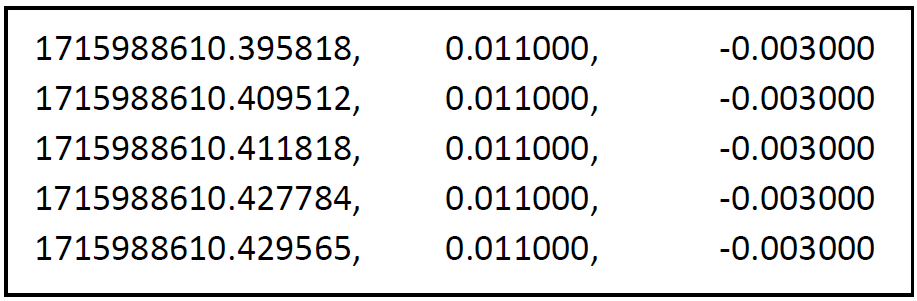
\includegraphics[width=4.16667in,height=\textheight,keepaspectratio]{images/media/77_1_scale_file.png}
\end{center}

A Scale File is created when a weight, greater than the minimum penguin
weight, is applied to one of the scales. This minimum weight
(\texttt{MIN\_PENGUIN\_WEIGHT}) is set in the APMS config file. See:
\hyperref[Configuringux5cux2520theux5cux2520APMS]{Configuring the APMS}.
The Scale File ends when the scale is empty for longer than a preset
time (\texttt{SCALE\_EMPTY\_TIME} in the APMS config file). The same
amount of time before the scale was triggered is also added to the end
of the file.

The scale files are unique in that their filenames contain a wealth of
information. A typical scale file filename looks like this:

\textbf{S20231206033841ROB.csv}

\begin{itemize}
\item
  Where:

  \begin{itemize}
  \item
    The ``S'' signifies it's a scale file (RIFD files start with ``R'')
  \item
    The date the follows in the format ``YYYYMMDDHHMMSS''
  \item
    In our example 03:38:41 on the 6\textsuperscript{th} of December
    2023
  \item
    Followed by the site code.

    \begin{itemize}
    \item
      STO = Stony Point
    \item
      BIR = Bird Island
    \item
      DYE = Dyer Island
    \item
      ROB = Robben Island
    \item
      DAS = Dassen Island
    \end{itemize}
  \end{itemize}
\end{itemize}

\section{Determining the Direction of a
penguin}\label{determining-the-direction-of-a-penguin}

An example of a Scale File is shown below. The top picture is Scale 1
(Colony Side) and the bottom picture is Scale 2 (Ocean Side). This shows
two penguins, jumping on Scale 1 first, then Scale 2. They are thus
heading out to the ocean. This is how the penguin direction is
determined.

\begin{figure}[H]

{\centering 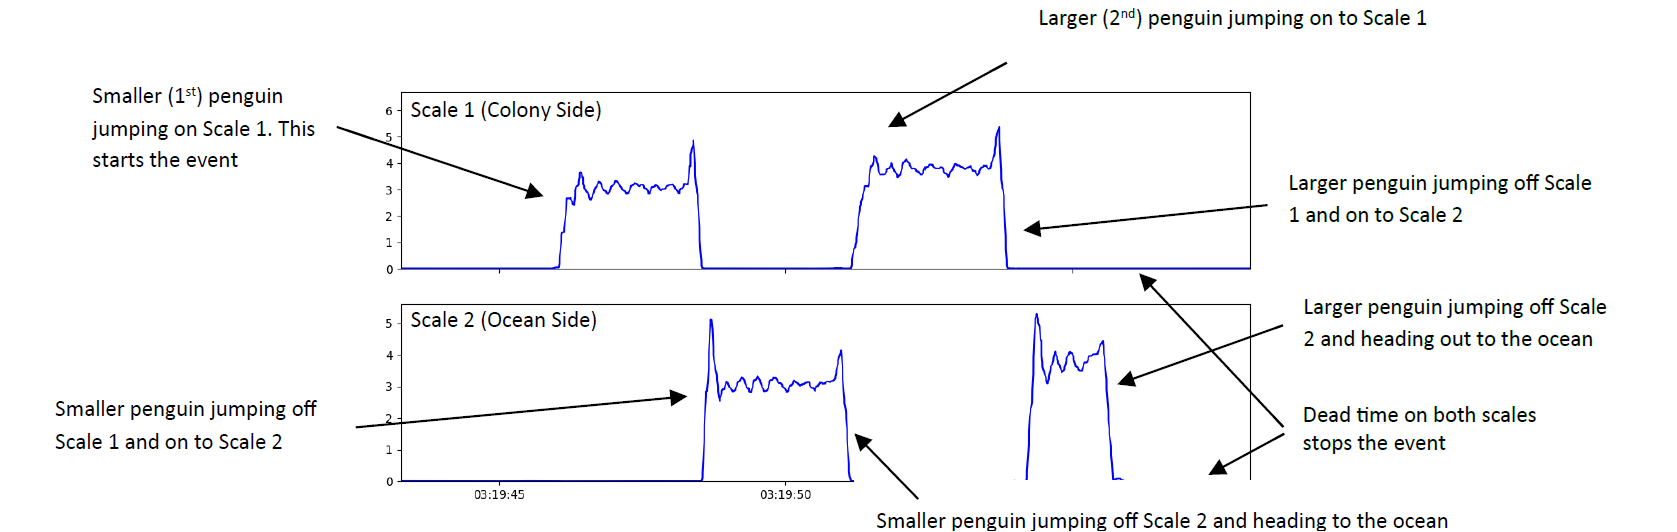
\includegraphics[width=7.29167in,height=\textheight,keepaspectratio]{images/media/77_0_scale_file.png}

}

\caption{\textbf{Figure 77.} Scale file plotted with weight on the
Y-axis and time on the X-axis. The top graph is colony side, and bottom
ocean side, indicating two penguins going out to sea.}

\end{figure}%

\section{Determining the Weight of a
penguin}\label{determining-the-weight-of-a-penguin}

Each Scale File consists of two events, one for each scale. The data is
analysed and a separate penguin list is generated for each scale. The
two lists are then compared and if certain checks are passed, they are
combined to form a penguin list for the entire Scale File.

\textbf{This hinges on the fact that we assume penguins will cross the
scales in single file and not go past each other. This is why it is
important to ensure the weighbridge and path is narrow enough to funnel
them one by one.}

Each scale event is broken up into sub events which are then analysed.
Below is a simple case with two sub events per scale. In this case, each
sub event contains only one weight. Every sub event has deadweight
before and after it. There will thus be one more deadweight than sub
events, in the event.

The example above is shown again, indicating the different weights
identified

\begin{figure}[H]

{\centering 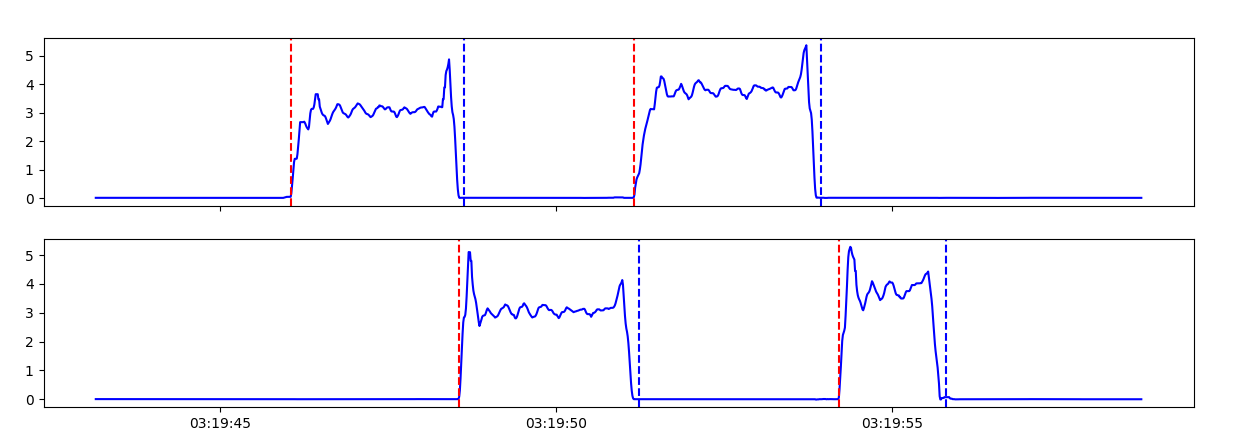
\includegraphics[width=6.25in,height=\textheight,keepaspectratio]{images/media/78_scale_file.png}

}

\caption{\textbf{Figure 78.} Scale file partitioned into sub events.}

\end{figure}%

\begin{itemize}
\tightlist
\item
  The weight inside each sub event is then identified and analysed.
\end{itemize}

The weight is categorised as one of the following:

\begin{itemize}
\item
  \textbf{Too Short:} Too little time spent on scale. This weight is not
  used.
\item
  \textbf{Static Weight:} Deadweight or animal stationary. Average
  taken.
\item
  \textbf{Dynamic Weight:} Not Static. Oscillatory. Explained below.
\end{itemize}

The first weight of the example above has been extracted from the sub
event and can be seen below. It is a \emph{Dynamic Oscillatory weight}
and the peaks are identified and used to determine the weight.

\begin{figure}[H]

{\centering 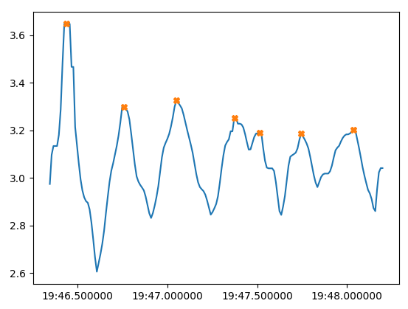
\includegraphics[width=4.16667in,height=\textheight,keepaspectratio]{images/media/79_scale_file.png}

}

\caption{\textbf{Figure 79.} Example of a dynamic oscillatory weight
reading.}

\end{figure}%

As noted in {[}REFERENCE{]}, as the penguin is walking, one can assume
the penguin's vertical velocity will be the same between two points one
period apart. We will choose the peaks as they are easy to identify. The
mass of the penguin during the event is constant and as the momentum is
given by mass times velocity, and the velocity is the same at the peaks,
we can say the momentum of the penguin in the vertical direction is the
same at the peaks. There is thus no change in momentum between the
peaks, i.e, the \ul{impulse is zero}. The impulse is given as the
integral of the force on the penguin, with respect to time.

\[J = \ \int_{}^{}{F_{net}(t)\ dt}\]

The net force on the penguin, at any point in time, is the force of the
scale on the penguin, minus the force of gravity on the penguin. (As
these are the only two forces acting on the penguin, ignoring air
resistance).

Also, the force of gravity on the penguin does not change as

\[F_{g} = m_{penguin}*g\]

both of which we assume are constant during the event.

If we take the impulse as zero between the peak at \(t_{1}\) and
\(t_{2}\), as discussed above, we get:

\[0 = \ \int_{t1}^{t2}{{(F}_{scale}(t) - F_{g})}dt\]

Where \(F_{scale\ }(t)\ \)is the force of the scale on the penguin.

We know the force of the penguin on the scale is opposite in sign but
equal in magnitude to the force of the scale on the penguin.

\[{\ \ F}_{penguin - on - scale} = - {\ \ F}_{scale}\]

Our scales provide \(m(t)\), the mass on the scale, recorded every 10ms.

We know

\[F_{penguin - on - scale}(t) = m(t)*g\]

We thus get:

\[{\ \ F}_{scale} = \  - m(t)*g\]

Substitution then gives \emph{\hfill\break
}\[0 = \ \int_{t1}^{t2}{\left( - m(t)*g - m_{penguin}*g \right)dt}\]

Solving for the mass of the penguin, \(m_{penguin}\) , we get:

\[m_{penguin} = \frac{\int_{t1}^{t2}{m(t)\ dt}}{t_{2} - t_{1}}\]

This integral is computed numerically and this is how the mass of the
penguin is determined using two peaks.

The penguin gives many steps and thus the mass is recalculated between
the peaks and an average is taken. More sophisticated techniques can be
used but this first approach gave adequate results (See: Weideman
\emph{et al.} in prep).

After all the sub events have been analysed for Scale 1 a penguin list
is created. The same process is then repeated for Scale 2. The two
penguin lists are then compared. If they contain the same number
penguins and if the difference in weight readings for the penguins are
low enough (\texttt{MAX\_SCALES\_DIFFERENCE\_ALLOWED} setting in the
config file), they will be added to the total penguin list for the Scale
File. The output of the algorithm for the two penguins above, can be
seen below (Fig. 80).

The time given is when the penguin first steps on the scale (Scale 1 if
going out to the ocean and Scale 2 if coming back from the ocean) As
there were no RFID tags picked up, the penguin ID 's are given as 0 and
1. This will be replaced by an RFID tag number if applicable. See
\hyperref[Assigningux5cux2520anux5cux2520RFIDux5cux2520Tagux5cux2520toux5cux2520aux5cux2520penguin]{Assigning
an RFID Tag to a penguin}.

Another example can be seen below, of three penguins walking over the
scales. The top graph is Scale 1 (Colony Side) and the bottom graph is
Scale 2 (Ocean Side). Note the peak on Scale 1 when both penguins were
on the scale. On Scale 2, one can see that one penguin was busy jumping
off as another was jumping on.

\begin{figure}[H]

{\centering 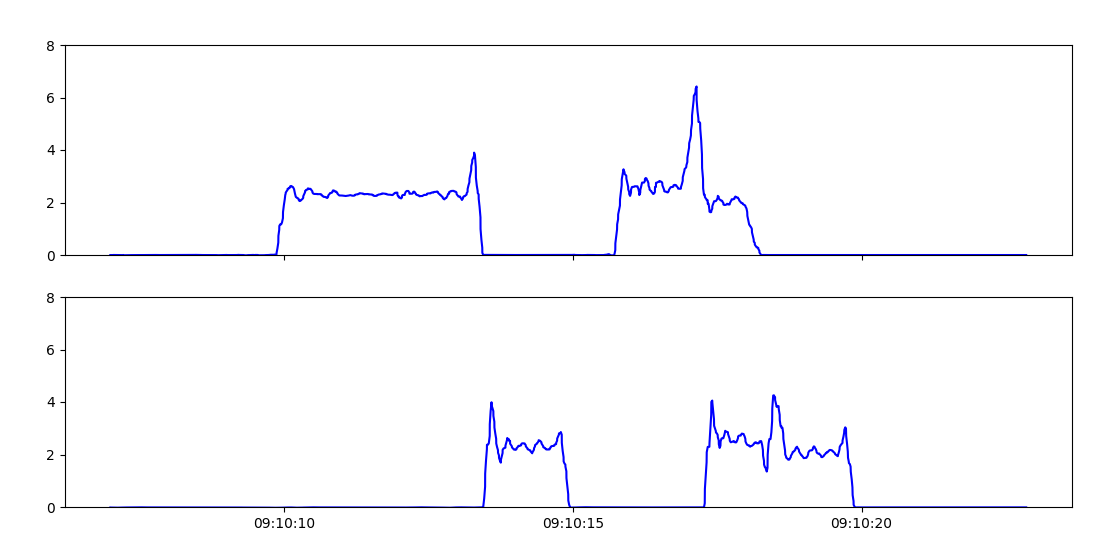
\includegraphics[width=7.29167in,height=\textheight,keepaspectratio]{images/media/80_scale_file.png}

}

\caption{\textbf{Figure 80.} Output of the weight algorithm for two
penguins crossing the weighbridge and heading out to sea.}

\end{figure}%

\begin{figure}[H]

{\centering 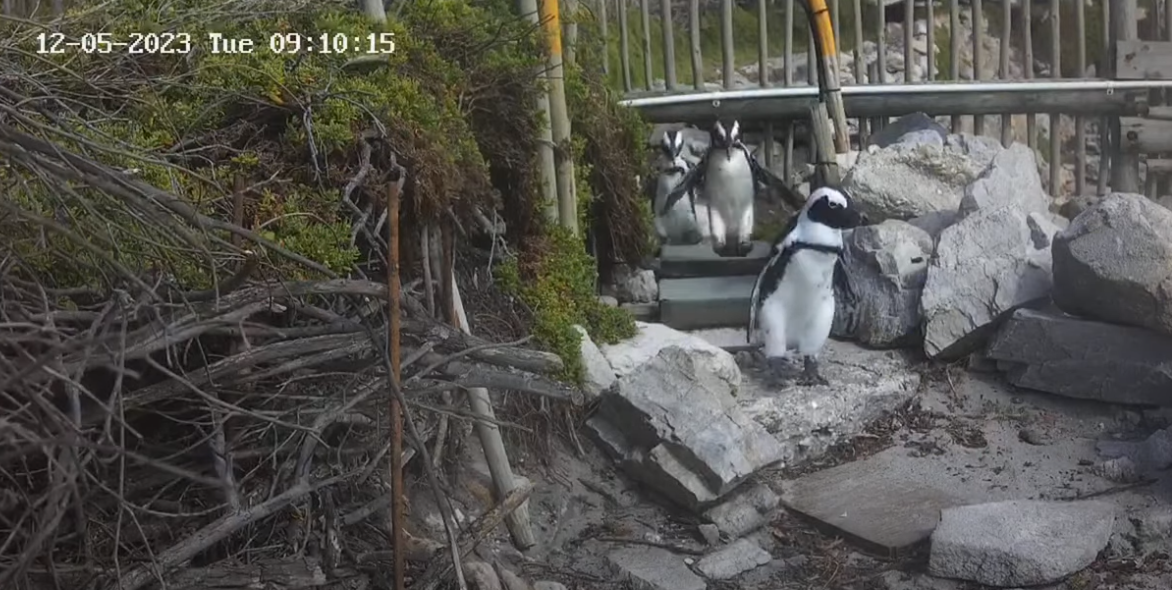
\includegraphics[width=7.29167in,height=\textheight,keepaspectratio]{images/media/image150.png}

}

\caption{\textbf{Figure 81.} Three penguins crossing the old weighbridge
at Stony Point.}

\end{figure}%

\begin{longtable}[]{@{}
  >{\centering\arraybackslash}p{(\linewidth - 10\tabcolsep) * \real{0.1667}}
  >{\centering\arraybackslash}p{(\linewidth - 10\tabcolsep) * \real{0.1667}}
  >{\centering\arraybackslash}p{(\linewidth - 10\tabcolsep) * \real{0.1667}}
  >{\centering\arraybackslash}p{(\linewidth - 10\tabcolsep) * \real{0.1667}}
  >{\centering\arraybackslash}p{(\linewidth - 10\tabcolsep) * \real{0.1667}}
  >{\centering\arraybackslash}p{(\linewidth - 10\tabcolsep) * \real{0.1667}}@{}}
\caption{Automated weighbridge measurements for penguins featured in
Fig. 81.}\label{tbl-penguin-weights}\tabularnewline
\toprule\noalign{}
\begin{minipage}[b]{\linewidth}\centering
Penguin ID
\end{minipage} & \begin{minipage}[b]{\linewidth}\centering
Weight (kg)
\end{minipage} & \begin{minipage}[b]{\linewidth}\centering
Weight Type
\end{minipage} & \begin{minipage}[b]{\linewidth}\centering
Date Time (UTC+2)
\end{minipage} & \begin{minipage}[b]{\linewidth}\centering
Direction
\end{minipage} & \begin{minipage}[b]{\linewidth}\centering
Scale Diff (kg)
\end{minipage} \\
\midrule\noalign{}
\endfirsthead
\toprule\noalign{}
\begin{minipage}[b]{\linewidth}\centering
Penguin ID
\end{minipage} & \begin{minipage}[b]{\linewidth}\centering
Weight (kg)
\end{minipage} & \begin{minipage}[b]{\linewidth}\centering
Weight Type
\end{minipage} & \begin{minipage}[b]{\linewidth}\centering
Date Time (UTC+2)
\end{minipage} & \begin{minipage}[b]{\linewidth}\centering
Direction
\end{minipage} & \begin{minipage}[b]{\linewidth}\centering
Scale Diff (kg)
\end{minipage} \\
\midrule\noalign{}
\endhead
\bottomrule\noalign{}
\endlastfoot
0 & 2.322 & avg\_dynamic & 2023-12-05 09:10:12 & Out to ocean &
-0.0071 \\
1 & 2.624 & avg\_dynamic & 2023-12-05 09:10:17 & Out to ocean &
-0.0373 \\
2 & 2.053 & avg\_dynamic & 2023-12-05 09:10:18 & Out to ocean &
-0.0318 \\
\end{longtable}

\section{Assigning an RFID Tag to a
penguin}\label{assigning-an-rfid-tag-to-a-penguin-1}

After the scale file is analysed and a list of penguins is generated,
RFID tags can be assigned. For each penguin a ``crossing time'' is
calculated. A penguin crossing is defined as the period between first
stepping on the scales until stepping off the scales. A single
``crossing \emph{time}'' is calculated as halfway through the penguin
crossing.

For each penguin, the crossing time is compared to the RFID timestamps
to check if an RFID tag was picked up close to when the penguin crossed
the scales. (\texttt{RFID\_TO\_PENGUIN\_INTERVAL} in the config file).
By default, \texttt{RFID\_TO\_PENGUIN\_INTERVAL} is set to 60 seconds.

The location of the RFID antenna is set in the config file for each
site. Look for \texttt{rfid\_location\ :\ middle\_only} near the bottom
of \texttt{config.py}. The default is \texttt{middle\_only}, as this is
the configuration for all new sites. This is not the case for older
sites, see later in this chapter.

When \texttt{middle\_only} is given as the RFID antenna location, and no
other RFID tags were recorded during the penguin's crossing, the
algorithm can assign a RFID tag number to the penguin based on the
following two scenarios

\begin{enumerate}
\def\labelenumi{\arabic{enumi}.}
\tightlist
\item
  The tag is picked up during the jump from one scale to the other.
\end{enumerate}

If a tag is picked up within the time period when the penguin is jumping
from one scale to the other, the tag number is assigned to that penguin.
This is also valid for a group of penguins, as we assume they move in
single file over the scales. This is why it is important to ensure they
move in single file when setting up the site, to avoid a penguin
overtaking another and causing the event to be discarded or worse, an
incorrect RFID tag assigned to a penguin. See example below (Fig. 82).

\begin{enumerate}
\def\labelenumi{\arabic{enumi}.}
\setcounter{enumi}{1}
\tightlist
\item
  The tag was picked up somewhere during the penguin's crossing. No
  other penguins crossing.
\end{enumerate}

Sometimes, due to various circumstances, the antenna will pick up the
tag too early, or even after the jump. If, however, we know the antenna
is placed in between the scales, and no other penguins were crossing at
the same time, we assume the tag belongs to that penguin.

Below is an example of two penguins heading out to the ocean. They each
trigger the BioMark RFID reader (red line in Fig. 82) as they jump from
Scale 1 (colony side) to Scale 2 (ocean side) and thus both have RFID
tag numbers assigned to them.

\begin{figure}[H]

{\centering 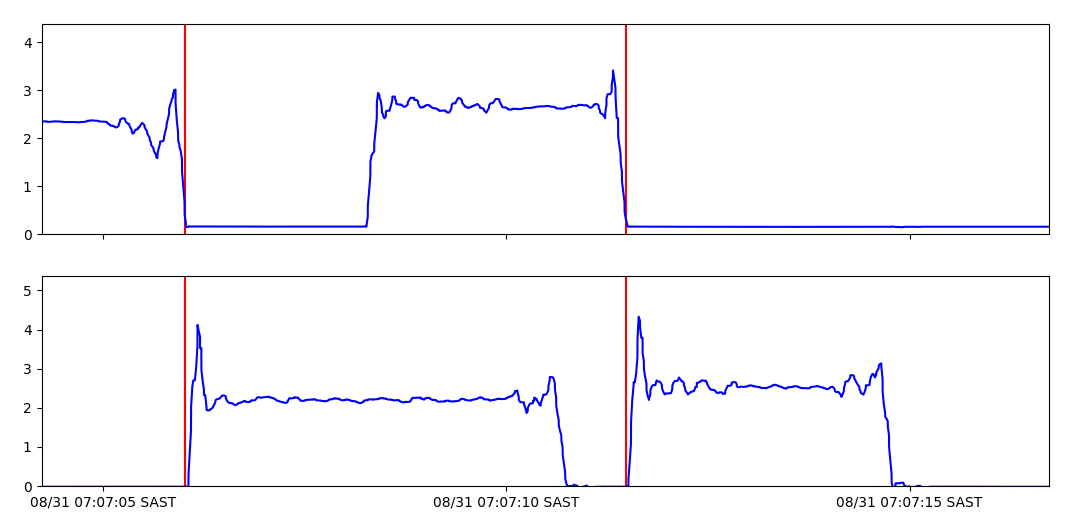
\includegraphics[width=7.29167in,height=\textheight,keepaspectratio]{images/media/82_scale_event.png}

}

\caption{\textbf{Figure 82.} Another example of two penguins going out
to see. Red line is when an RFID PIT-tag was recorded.}

\end{figure}%

\begin{tcolorbox}[enhanced jigsaw, left=2mm, toptitle=1mm, breakable, opacitybacktitle=0.6, title={Basic Validation Configuration Checks}, colback=white, opacityback=0, rightrule=.15mm, leftrule=.75mm, colbacktitle=quarto-callout-note-color!10!white, bottomtitle=1mm, titlerule=0mm, coltitle=black, colframe=quarto-callout-note-color-frame, arc=.35mm, bottomrule=.15mm, toprule=.15mm]

The algorithm verifies all of the following conditions before accepting
a reading. These parameters can all be configured in the config file:

\begin{itemize}
\tightlist
\item
  \textbf{\texttt{RFID\_TO\_PENGUIN\_INTERVAL}} \emph{(Default:
  \texttt{60\ sec})}\\
  Tag detected close to the penguin crossing time.
\item
  \textbf{\texttt{RFID\_ISOLATION\_INTERVAL}} \emph{(Default:
  \texttt{5\ minutes})}\\
  Tag was the only one detected within this window.
\item
  \textbf{\texttt{SCALE\_FILE\_ISOLATION\_INTERVAL}} \emph{(Default:
  \texttt{60\ seconds})}\\
  Only one scale file generated within this window.
\item
  \textbf{Single Penguin Rule} \emph{(Enforced by algorithm)}\\
  There must be only one penguin recorded in the generated scale file.
\end{itemize}

\end{tcolorbox}

\section{Error Handling}\label{error-handling-1}

Penguins are wild animals and they do not always walk nicely over the
scales. Numerous situations can give rise to a scale file not being
processed. A fault with the scale could also lead to data files that can
not be processed by the algorithm. When the algorithm discards the file,
it moves it to an ``error'' directory with the name of the error. These
files can then be viewed separately to learn more. The error directories
are in the ``processed'' folder. See below for the path.

\textbf{\emph{\textasciitilde\textbackslash apms\_data\_processing\textbackslash data\textbackslash processed\textbackslash{}
{[}site name{]} \textbackslash{} {[}YEAR{]} \textbackslash{}
{[}YYYYMMDD{]} \textbackslash{} {[}ERROR DIRECTORY{]}}}

Note that even though these are called ``error'' directories, it does
not mean there is a fault. For instance, if another animal triggers the
scale, the algorithm should detect that and move it to the
``no\_penguins'' error directory. Many of these errors are based on
parameters in the config file. See
\hyperref[Configuringux5cux2520theux5cux2520APMS]{Configuring the APMS}.

When a site is not performing as expected, viewing these directories can
often give clues as to what is wrong.

This can be added to, with different error states added as required. The
current error directories are as follows:

\begin{longtable}[]{@{}
  >{\raggedright\arraybackslash}p{(\linewidth - 2\tabcolsep) * \real{0.5000}}
  >{\raggedright\arraybackslash}p{(\linewidth - 2\tabcolsep) * \real{0.5000}}@{}}
\caption{Summary of scale error directories and their
definitions.}\label{tbl-error-directories}\tabularnewline
\toprule\noalign{}
\begin{minipage}[b]{\linewidth}\raggedright
Error Directory
\end{minipage} & \begin{minipage}[b]{\linewidth}\raggedright
Reason
\end{minipage} \\
\midrule\noalign{}
\endfirsthead
\toprule\noalign{}
\begin{minipage}[b]{\linewidth}\raggedright
Error Directory
\end{minipage} & \begin{minipage}[b]{\linewidth}\raggedright
Reason
\end{minipage} \\
\midrule\noalign{}
\endhead
\bottomrule\noalign{}
\endlastfoot
timing\_jump & Large time difference between samples in scale file
(greater than 1 second). \\
frequency\_error & Scale sampling period is not correct. Set in config
file: \texttt{MAX\_AVG\_SAMPLING\_PERIOD} and
\texttt{MIN\_AVG\_SAMPLING\_PERIOD}. \\
no\_sub\_events & No sub events found in scale file. \\
unequal\_num\_penguins & Number of penguins determined for Scale 1
differs from the number determined for Scale 2. \\
no\_penguins & List of penguins for scale 1 and scale 2 are both
empty. \\
direction\_error & Different number of penguins going out to the ocean
than coming back. \\
penguin\_weight\_error & Algorithm could not determine a weight from the
provided data. \\
weight\_too\_high & Weight was recorded as more than 3x max penguin
weight. Set in config file: \texttt{MAX\_PENGUIN\_WEIGHT}. \\
overload & Weight exceeding scale maximum. Set in config file:
\texttt{SCALE\_OVERLOAD}. \\
duplicate\_timestamps & Weights with the same timestamp found in scale
file. \\
large\_penguin\_weight\_difference & Large difference in weight between
scale 1 and scale 2. Set in config file:
\texttt{MAX\_SCALES\_DIFFERENCE\_ALLOWED}. \\
no\_dead\_weight\_events & No periods found where the scale was reading
a stationary dead weight. \\
large\_dead\_weight & Weight on empty scale before or after event is
higher than the allowed ``dead weight''. Set in config file:
\texttt{MAX\_DEAD\_WEIGHT}. \\
large\_dead\_weight\_difference & Difference between the dead weight on
the scale before the penguin jumps on and after it jumps off is too
large. Set in config file: \texttt{MAX\_DEADWEIGHT\_DIFF}. \\
negative\_jump\_time & Time calculation of time taken to jump from one
scale to the other gave a negative result. \\
negative\_time\_on\_scale & Time of penguin jumping on to the scale is
\ul{after} time of penguin jumping off scale. \\
\end{longtable}

\section{APMS Dashboard}\label{apms-dashboard}

The APMS Dashboard allows the operator to view the health of the system
at each site. The Dashboard uses the processed data files to display
penguin data. The data processing script must thus be fully functioning
before setting up the Dashboard. See
\hyperref[Dataux5cux2520Processingux5cux2520Scriptux5cux2520Usage]{Data
Processing Script Usage}. The instructions that follow explains how to
install the dashboard on a machine running Ubuntu.

\begin{figure}[H]

{\centering 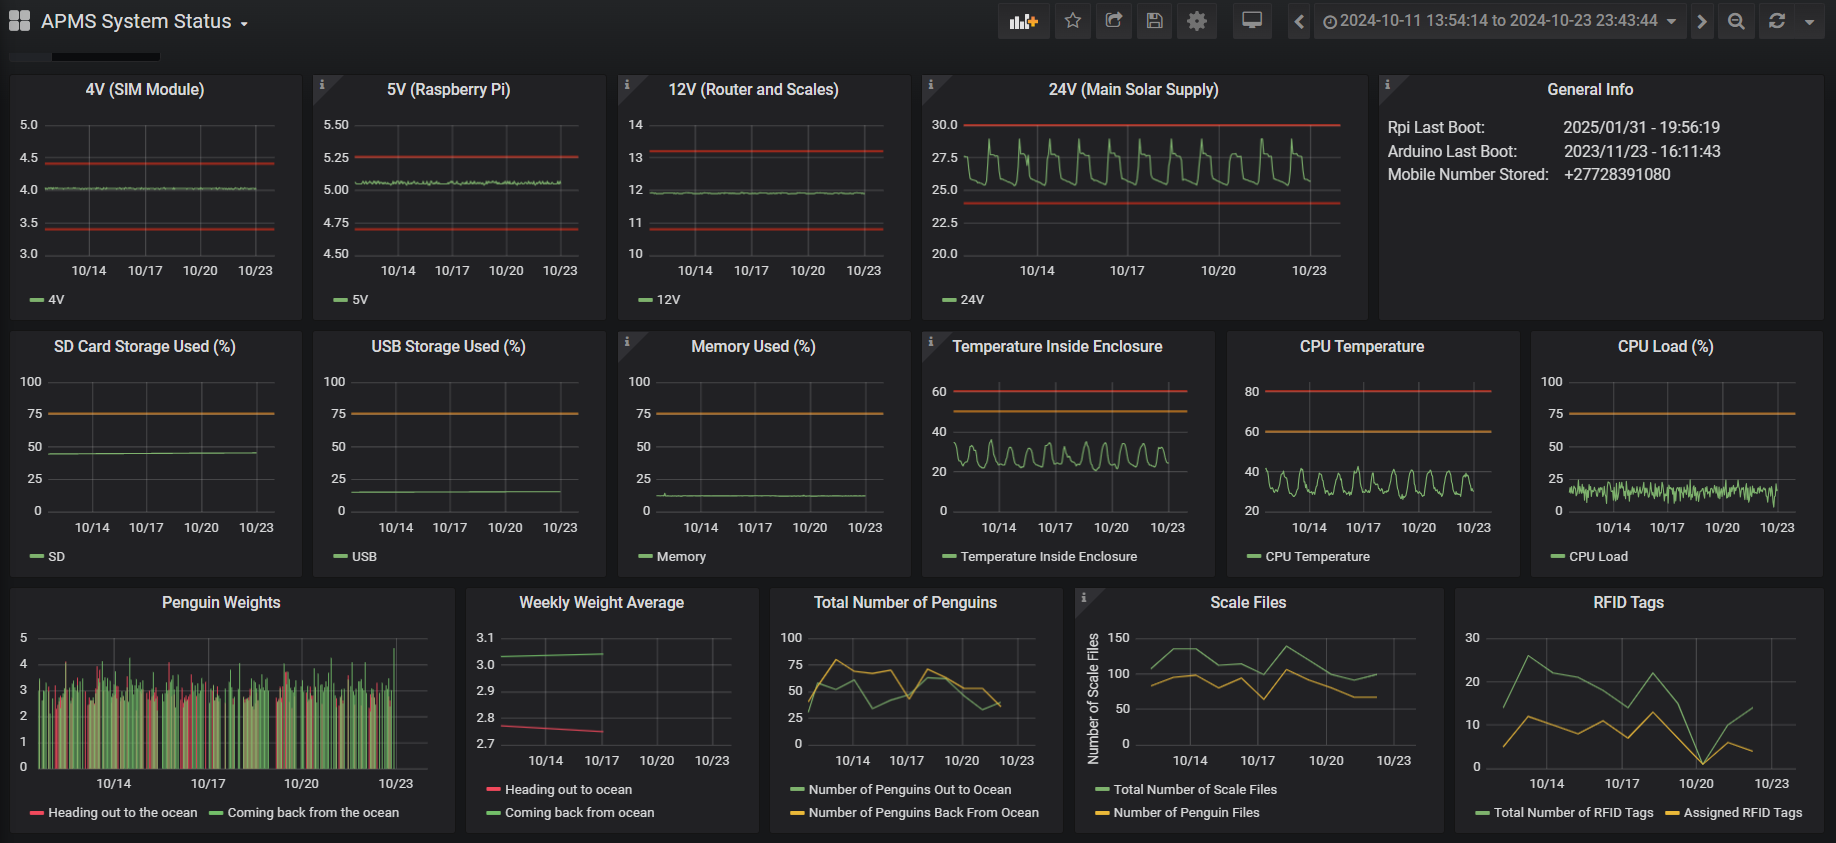
\includegraphics[width=7.29167in,height=\textheight,keepaspectratio]{images/media/83_dash.png}

}

\caption{\textbf{Figure 83.} Screenshot of the APMS Dashboard.}

\end{figure}%

\subsection{Install Ubuntu}\label{install-ubuntu}

To install Ubuntu, use the Rufus application and write an Ubuntu image
to it. The current versions are stored on the cloud, replace in future
with newer versions if needed.

\begin{itemize}
\item
  Rufus can be downloaded here: \href{https://rufus.ie/en/}{Rufus
  download}

  \begin{itemize}
  \tightlist
  \item
    The software is also saved here on the server:
    \emph{s3://apmsbirdlife/APMS/software/Rufus\_and\_Ubuntu/rufus-4.1.exe}
  \end{itemize}
\item
  Ubuntu can be found at
  \href{https://ubuntu.com/download/desktop}{Download Ubuntu}
\item
  Download both rufus and the Ubuntu image to a local directory on your
  machine.
\item
  Get a Flash Drive. \textbf{Note all data will be deleted on this Flash
  Drive.}
\item
  Run Rufus and select the Flash Drive under ``\emph{device''}.
\item
  Under ``\emph{boot selection''} click''\emph{SELECT}'' and select the
  Ubuntu image you downloaded.
\item
  Leave all the other settings as they are and click ``\emph{START''}.
  This will create the Ubuntu Flash Drive.
\end{itemize}

Insert the Flash Drive into the machine where Ubuntu will be installed,
reboot and follow the onscreen instructions to install Ubuntu. After
successfully installing Ubuntu, you will restart and go into the
Desktop. For more information on installing Ubuntu, see this online
\href{https://ubuntu.com/tutorials/install-ubuntu-desktop\#1-overview}{tutorial}.

\subsection{Install Influx DB}\label{install-influx-db}

InfluxDB is the database that will hold all the processed data, for
displaying on the Dashboard.

The instructions below will be executed from a terminal.

\begin{itemize}
\tightlist
\item
  To open a terminal from anywhere on Ubuntu, press \textbf{CTRL + ALT +
  t}
\end{itemize}

Run the following commands to install and configure InfluxDB:

\begin{Shaded}
\begin{Highlighting}[]
\CommentTok{\# Update local package index}
\FunctionTok{sudo}\NormalTok{ apt{-}get update}

\CommentTok{\# Install the InfluxDB database service}
\FunctionTok{sudo}\NormalTok{ apt install }\AttributeTok{{-}y}\NormalTok{ influxdb}

\CommentTok{\# Start the InfluxDB service immediately}
\FunctionTok{sudo}\NormalTok{ systemctl start influxdb}

\CommentTok{\# Enable InfluxDB to launch automatically on system boot}
\FunctionTok{sudo}\NormalTok{ systemctl enable influxdb}

\CommentTok{\# Install the InfluxDB command{-}line client CLI tool}
\FunctionTok{sudo}\NormalTok{ apt install }\AttributeTok{{-}y}\NormalTok{ influxdb{-}client}
\end{Highlighting}
\end{Shaded}

\subsection{Install Grafana Server}\label{install-grafana-server}

Grafana is the graphical interface to display the data in the database,
what the user see's and interacts with. To run the Grafana Dashboard, a
Grafana server should be installed and configured.

\begin{Shaded}
\begin{Highlighting}[]
\CommentTok{\# Update local package index}
\FunctionTok{sudo}\NormalTok{ apt{-}get update}

\CommentTok{\# Install the Grafana server package}
\FunctionTok{sudo}\NormalTok{ apt{-}get install }\AttributeTok{{-}y}\NormalTok{ grafana}

\CommentTok{\# Start the Grafana server service immediately}
\FunctionTok{sudo}\NormalTok{ systemctl start grafana{-}server}

\CommentTok{\# Enable Grafana server to launch automatically on system boot}
\FunctionTok{sudo}\NormalTok{ systemctl enable grafana{-}server.service}
\end{Highlighting}
\end{Shaded}

\subsection{Set up the Dashboard}\label{set-up-the-dashboard}

To display anything on the Dashboard, the data must first be processed.
This is explained in Data Processing Script Usage.

The script \texttt{dashboard.py} is then used to read the processed data
into InfluxDB, with it eventually being displayed on Grafana. The IP
address is needed to configure the Grafana dashboard. To find the IP
address of the machine where Grafana is running, go into a terminal and
type:

\begin{Shaded}
\begin{Highlighting}[]
\ExtensionTok{ifconfig}
\end{Highlighting}
\end{Shaded}

Below is an example showing the output of \texttt{ifconfig} and where to
find the IP address.

\begin{figure}[H]

{\centering 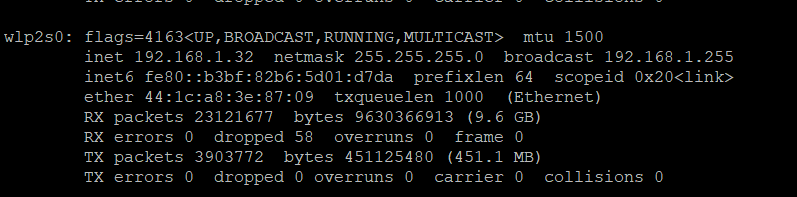
\includegraphics[width=6.25in,height=\textheight,keepaspectratio]{images/media/84_dash.png}

}

\caption{\textbf{Figure 84.} Finding the IP address when setting up a
new APMS Dashboard.}

\end{figure}%

Add this IP address to the \texttt{HOST\_IP} parameter in the
configuration file.

The usage of the dashboard script is the same as
\texttt{process\_data.py}. That is:
\texttt{python3\ dashboard.py\ SITE\ DATE\_RANGE}. See*
\hyperref[Dataux5cux2520Processingux5cux2520Scriptux5cux2520Usage]{Data
Processing Script Usage} for examples.

In a browser of any computer on the network, including the one where
Grafana has been installed type the IP address, followed by `:3000'. For
example: \url{http://192.168.1.32:3000}.

This will open the Grafana page. If prompted for a password, enter
``admin'' for username and ``admin'' for password. This password can be
changed if required.

Grafana must now be configured to display data from InfluxDB. Click on
settings, then ``Add data sources''. Select InfluxDB and under ``URL''
enter the IP address of the server, or just \url{http://localhost} if it
is the same machine as where InfluxDB is installed.

\begin{figure}[H]

{\centering 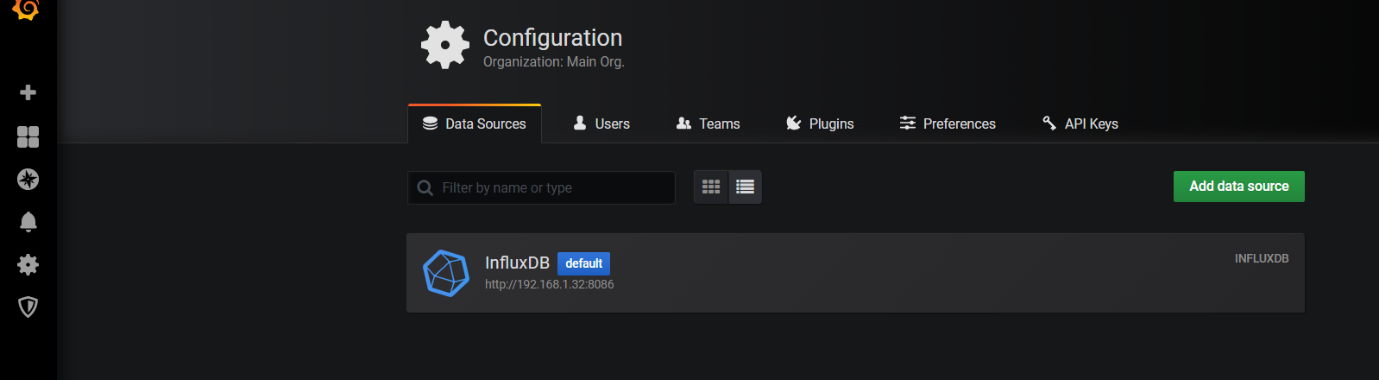
\includegraphics[width=6.25in,height=\textheight,keepaspectratio]{images/media/85_grafana.png}

}

\caption{\textbf{Figure 85.} Configuring InfluxDB on Grafana.}

\end{figure}%

\begin{figure}[H]

{\centering 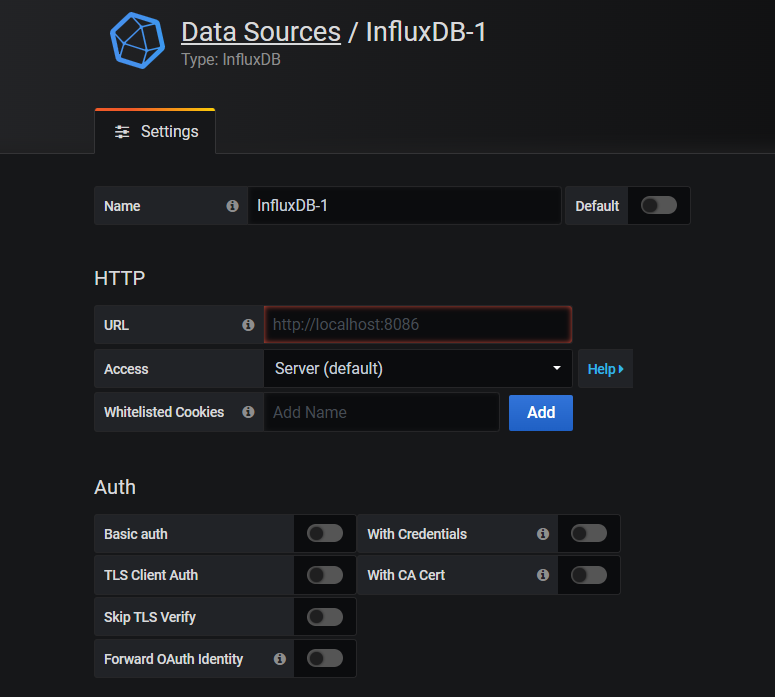
\includegraphics[width=4.16667in,height=\textheight,keepaspectratio]{images/media/86_grafana.png}

}

\caption{\textbf{Figure 86.} Configuring InfluxDB on Grafana.}

\end{figure}%

The final step is to load the APMS Dashboard. Click on the PLUS found in
the top left area and click ``Import''. In the text box provided, copy
and paste the JSON code from the APMS\_Dashboard.JSON file located at:
\textasciitilde/apms\_data\_processing/APMS\_Dashboard.JSON.

\begin{figure}[H]

{\centering 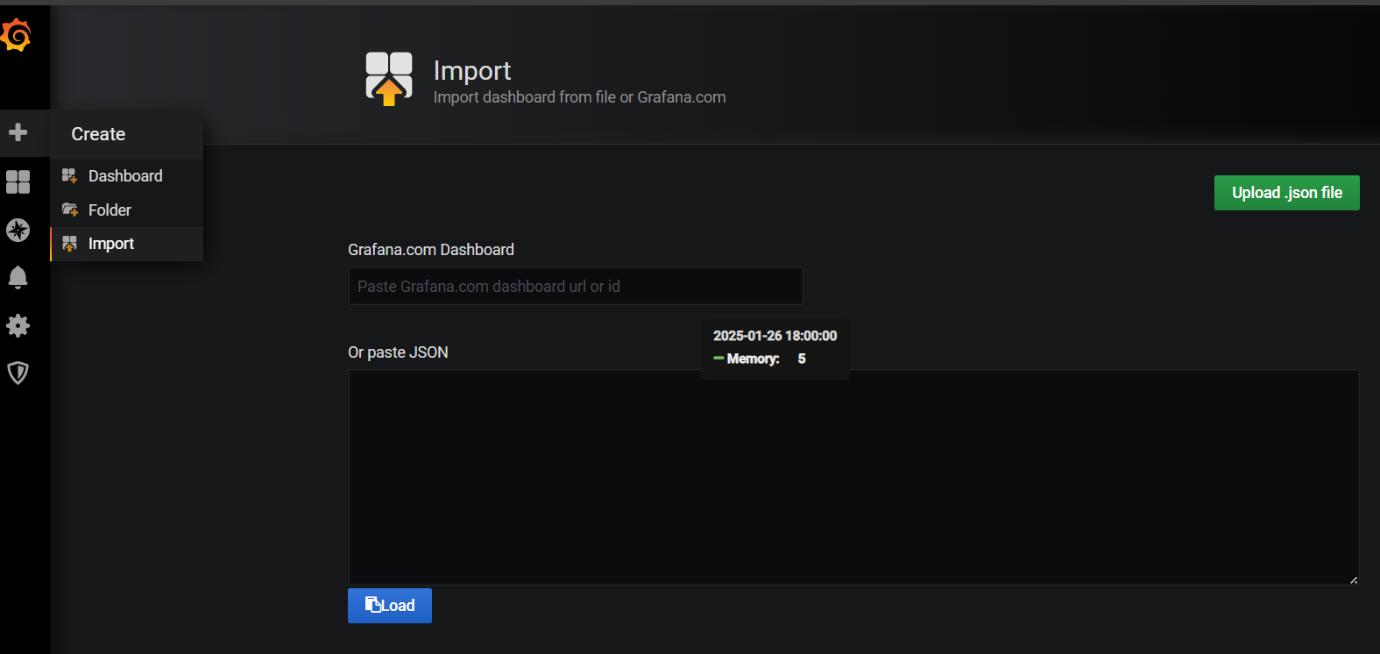
\includegraphics[width=6.25in,height=\textheight,keepaspectratio]{images/media/87_grafana.png}

}

\caption{\textbf{Figure 87.} Configuring InfluxDB on Grafana.}

\end{figure}%

Click Load. If data has been loaded into the database as described
earlier, using the \texttt{dashboard.py} script, it should be displayed
on the Dashboard.

\subsection{Automatic Dashboard
Update}\label{automatic-dashboard-update}

The script \texttt{process\_and\_display.sh} can be added to the crontab
to enable the system to process the data from all the sites and load it
to influx. For more information regarding the crontab, see
\hyperref[Configureux5cux2520theux5cux2520Crontab]{Configure the
Crontab}. Note that whenever new sites are added or removed that this
file has to be edited to reflect those changes.

Edit the Crontab:

\begin{Shaded}
\begin{Highlighting}[]
\FunctionTok{crontab} \AttributeTok{{-}e}
\end{Highlighting}
\end{Shaded}

Add this line to the bottom:

\begin{Shaded}
\begin{Highlighting}[]
\ExtensionTok{0}\NormalTok{ 6 }\PreprocessorTok{*} \PreprocessorTok{*} \PreprocessorTok{*}\NormalTok{ /usr/bin/bash \textasciitilde{}/apms\_data\_processing/process\_and\_display.sh}
\end{Highlighting}
\end{Shaded}

This will run the script at 6 AM every morning and update the dash.

\chapter{Maintenance}\label{maintenance}

When visiting a site always remember to log everything you do, even
though it might seem insignificant.

Check the following an:

\begin{itemize}
\item
  Tighten stay ropes (where applicable)
\item
  Check outdoor router antennas and masts are secure (where applicable)
\item
  Check for water ingress into the Skitch Box
\item
  Check RFID antenna is still in good condition
\item
  Check the height at which an RFID test tag is picked up.
\end{itemize}

\section{Cleaning and Checking the
scales}\label{cleaning-and-checking-the-scales}

\begin{itemize}
\item
  Clean the scales whenever visiting the site. As long as very little
  pressure is applied to the scales themselves, the system does not need
  to be turned off and no penguins will be registered
\item
  Check around the scales and ensure no branches or debris are touching
  the scale pans. Anything touching the pans on the sides will alter the
  weight reading. Sand on top of the scales (if not too excessive) is
  not a problem.
\item
  Check that the canvas is still in good condition and not torn/peeling
  off. Replace as necessary.
\end{itemize}

\section{Routine Calibration of
Scales}\label{routine-calibration-of-scales}

R\&D Weighing recommends the scales be calibrated every 3 to 4 months to
ensure accuracy. However, some sites may require you to calibrate it
more often, and when the equipment starts getting older it's recommended
to calibrate more frequently. Version 1 of the APMS used the Laumas
TLB485 scale indicators whereas as of 2026 BirdLife has moved on to
using the General Measure GMT-X1 indicators which has more
functionalities. Below are the calibration instructions for both of
these. Always stop the \texttt{scales.py} script before starting with
calibrations.

\begin{Shaded}
\begin{Highlighting}[]
\FunctionTok{sudo}\NormalTok{ systemctl stop scales}
\end{Highlighting}
\end{Shaded}

\subsection{Calibration Data Sheet}\label{calibration-data-sheet}

A data sheet for field use can be downloaded from here:

\begin{itemize}
\item
  \href{_book/files/APMS_Calibration_datasheet.pdf}{APMS Calibration
  Datasheet (PDF)}
\item
  \href{_book/files/APMS_Calibration_datasheet.docx}{APMS Calibration
  Datasheet (Word)}
\end{itemize}

\subsection{General Measure GMT-X1
Indicators}\label{general-measure-gmt-x1-indicators}

To check if the system needs to be calibrated, place a 1kg and 5kg (6kg
combined) weight on each scale and observe the readings on the scale
indicators. If the reading is out by more than 5g, recalibrate. The wind
can have a huge influence on the scales and thus \ul{only calibrate on
good weather days}.

There are two scales at every site: Scale 1 (colony side) and Scale 2
(ocean side). Both are zeroed (tared) and calibrated in exactly the same
way, one after the other. Follow the steps below in order and record
every reading on the data sheet as you go, do not rely on memory.

\subsubsection{Record BEFORE readings (no calibration
yet)}\label{record-before-readings-no-calibration-yet}

First ensure the \texttt{scales.py} script has been stopped before
recording weight readings. With the scale in its current, uncalibrated
state, record the reading shown for each of the following, in this
order:

\begin{itemize}
\item
  No weight on scale 1 --- record the reading.
\item
  No weight on scale 2 --- record the reading.
\item
  Place the 1 kg weight on scale 1 --- record the reading.
\item
  Place the 1 kg weight on scale 2 --- record the reading.
\item
  Remove the 1 kg weight. Place the 5 kg weight on scale 1 --- record
  the reading.
\item
  Place the 5 kg weight on scale 2 --- record the reading.
\item
  Place the 1 kg and 5 kg weights together on scale 1 (i.e., 6 kg) ---
  record the reading.
\item
  Place the 1 kg and 5 kg weights together on scale 2 (i.e., 6 kg) ---
  record the reading.
\item
  Remove all weights from the scale.
\end{itemize}

\subsubsection{Clean the scales}\label{clean-the-scales}

Remove any sand build up, sticks or debris that are on or around the
scales. To do this, remove the scale pans and sweep out the sand that's
accumulated with your fingers or with a paint brush. Take care when you
work around the cables as strong pressure on the cables can break or
damage them and then the entire scale/loadcell would need to be
replaced.

\subsubsection{Zero (tare) the scales}\label{zero-tare-the-scales}

We will first zero scale 1 (colony side) and then the exact same steps
will be done for scale 2 (ocean side).

\begin{enumerate}
\def\labelenumi{\arabic{enumi}.}
\item
  Press the Enter button (\textbf{ENT}) to open the menu.
\item
  Press the right arrow to go to \textbf{2xx Weight\&CAL} and press
  Enter (\textbf{ENT}).

  \begin{figure}[H]

  {\centering 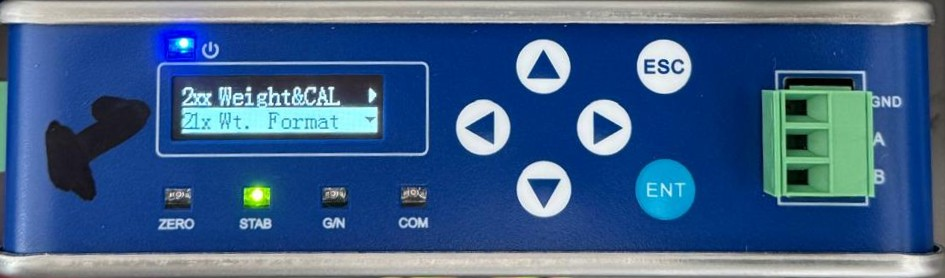
\includegraphics[width=5.72917in,height=\textheight,keepaspectratio]{images/media/89_weight_cal_menu.jpeg}

  }

  \caption{\textbf{Figure 89.} Selecting 2xx Weight\&CAL from the main
  menu.}

  \end{figure}%
\item
  Press the down arrow to go to \textbf{22x CAL Zero} and press Enter
  (\textbf{ENT}).

  \begin{figure}[H]

  {\centering 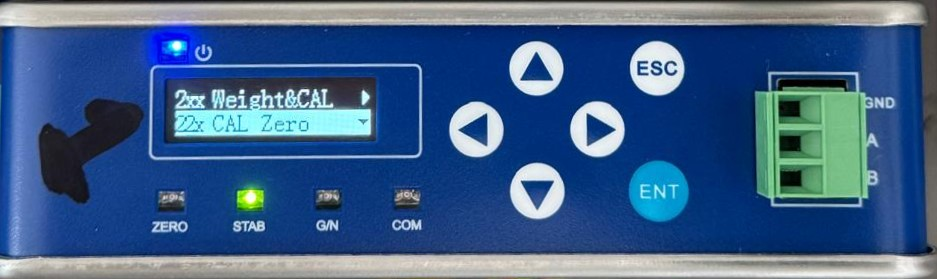
\includegraphics[width=5.72917in,height=\textheight,keepaspectratio]{images/media/90_cal_zero_menu.jpeg}

  }

  \caption{\textbf{Figure 90.} Selecting 22x CAL Zero from the
  Weight\&CAL menu.}

  \end{figure}%
\item
  It should now display \textbf{221 Auto Capture} --- press Enter
  (\textbf{ENT}).

  \begin{figure}[H]

  {\centering 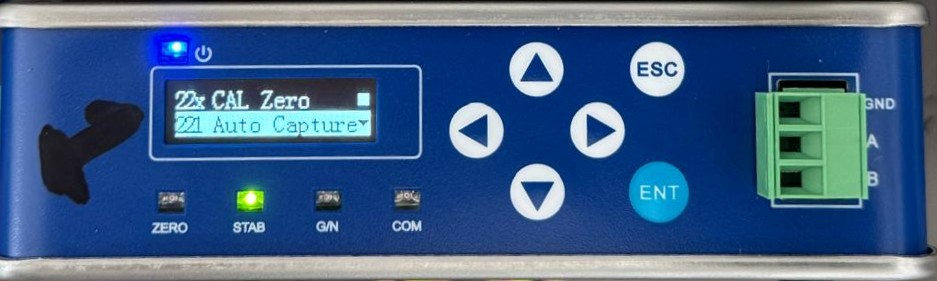
\includegraphics[width=5.72917in,height=\textheight,keepaspectratio]{images/media/91_auto_capture.jpeg}

  }

  \caption{\textbf{Figure 91.} Selecting 211 Auto Capture.}

  \end{figure}%
\item
  It should now display the weight reading in millivolts. Wait for a
  drop in the wind, or for the green stable weight reading light
  (\textbf{STAB}) to come on, then press Enter (\textbf{ENT})
  immediately to set the new zero point.

  \begin{figure}[H]

  {\centering 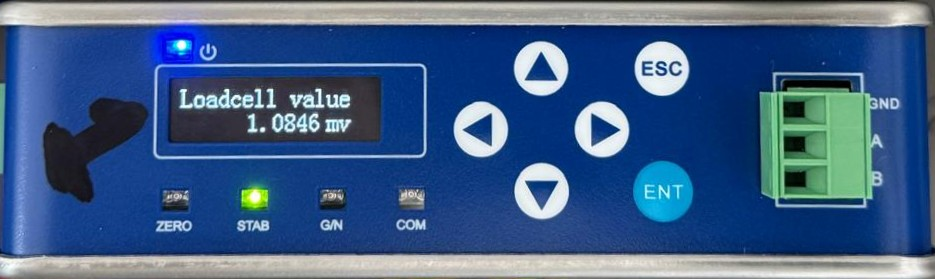
\includegraphics[width=5.72917in,height=\textheight,keepaspectratio]{images/media/92_zero_millivolts.jpeg}

  }

  \caption{\textbf{Figure 92.} Millivolt reading displayed while zeroing
  the scale.}

  \end{figure}%
\item
  You should see \textbf{Set Successfully} displayed on the screen and
  it should then return to the \textbf{22x CAL Zero} menu. Press Escape
  (\textbf{ESC}) to go back to the previous menu (\textbf{2xx
  Weight\&CAL}) for calibration (Step 5 below).

  \begin{figure}[H]

  {\centering 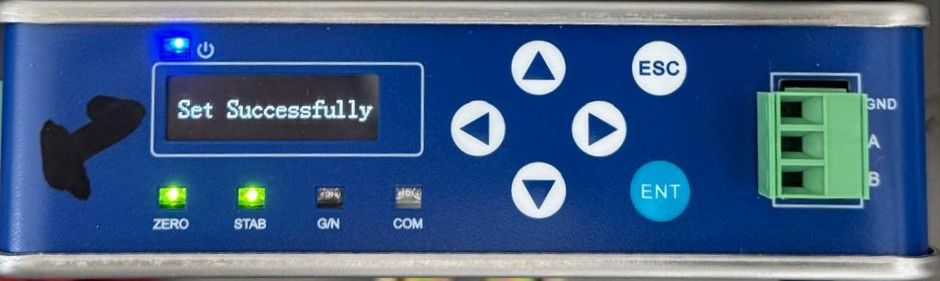
\includegraphics[width=5.72917in,height=\textheight,keepaspectratio]{images/media/93_set_successfully.jpeg}

  }

  \caption{\textbf{Figure 93.} Set Successfully confirmation screen.}

  \end{figure}%
\item
  Once you have zeroed (tared) scale 1, \textbf{repeat the exact same
  steps for scale 2.}
\end{enumerate}

\subsubsection{Calibrate the scales}\label{calibrate-the-scales}

We will first calibrate scale 1 (colony side) and then the exact same
steps will be done for scale 2 (ocean side).

\begin{enumerate}
\def\labelenumi{\arabic{enumi}.}
\item
  In the \textbf{2xx Weight\&CAL} menu, go down to \textbf{23x CAL
  Weight} and press Enter (\textbf{ENT}).

  \begin{figure}[H]

  {\centering 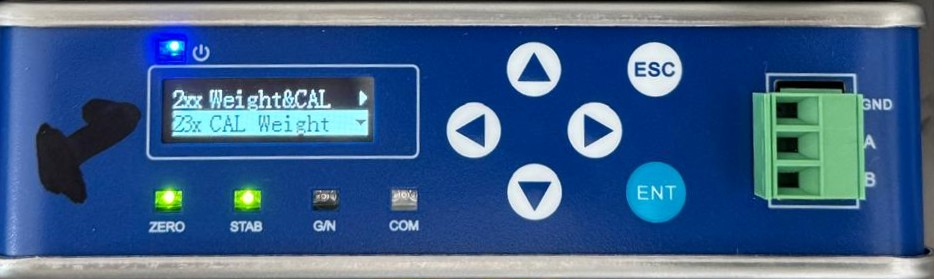
\includegraphics[width=5.72917in,height=\textheight,keepaspectratio]{images/media/94_cal_weight_menu.jpeg}

  }

  \caption{\textbf{Figure 94.} Selecting 23x CAL Weight from the
  Weight\&CAL menu.}

  \end{figure}%
\item
  You should now see \textbf{231 Weight CP1} displayed on the screen,
  press Enter (\textbf{ENT}).

  \begin{figure}[H]

  {\centering 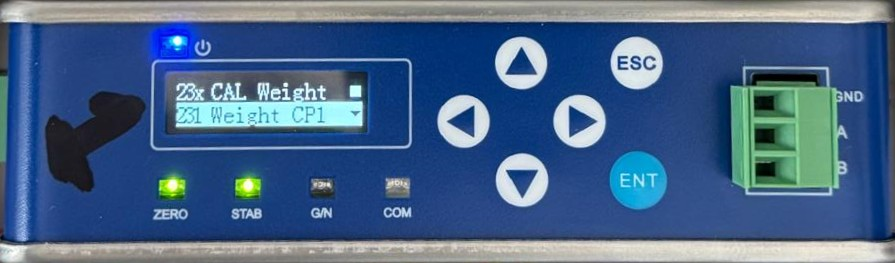
\includegraphics[width=5.72917in,height=\textheight,keepaspectratio]{images/media/95_weight_cp1.jpeg}

  }

  \caption{\textbf{Figure 95.} Selecting 231 Weight CP1.}

  \end{figure}%
\item
  You will see the millivolts as read by the loadcell displayed at the
  top of the screen. At the bottom, it will first show 000.000. Put the
  1 kg weight on scale 1. You will note that the millivolts have
  increased. \ul{Note the millivolts may be slightly different than the
  picture below.}

  \begin{figure}[H]

  {\centering 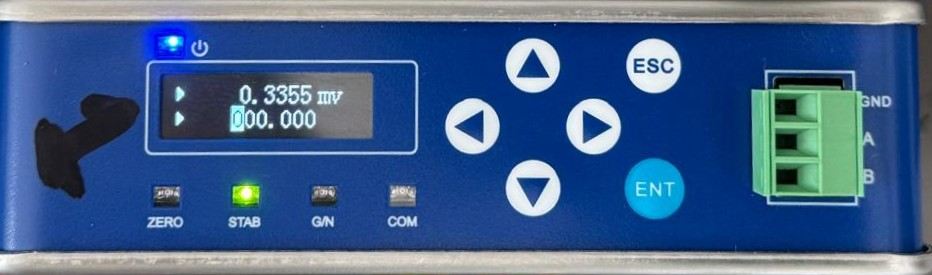
\includegraphics[width=5.72917in,height=\textheight,keepaspectratio]{images/media/96_1kg_millivolts.jpeg}

  }

  \caption{\textbf{Figure 96.} Millivolt reading increasing once the 1
  kg weight is placed on the scale.}

  \end{figure}%
\item
  Use the right arrow to move the cursor to the third 0 and then press
  the up arrow to adjust it to the weight that's on the scale, i.e., 1
  kg.

  \begin{figure}[H]

  {\centering 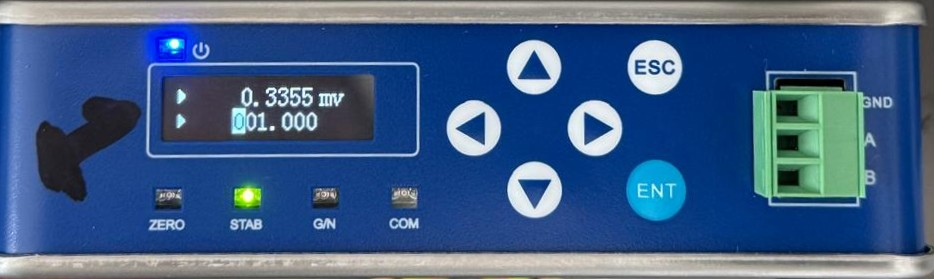
\includegraphics[width=5.72917in,height=\textheight,keepaspectratio]{images/media/97_1kg_adjust_cursor.jpeg}

  }

  \caption{\textbf{Figure 97.} Adjusting the displayed value to match
  the weight on the scale.}

  \end{figure}%
\item
  As soon as you see the green stable weight (\textbf{STAB}) light come
  on, or note a break in the wind, press Enter (\textbf{ENT}). It should
  now read \textbf{Set Successfully} on the screen (see Figure 93).
\item
  You have now successfully calibrated scale 1 with a 1 kg weight.
  Repeat the above steps with a 5 kg weight following the steps below.
\item
  You should see \textbf{231 Weight CP1} displayed on the screen again
  after you successfully calibrated it in the previous step. Press the
  down arrow once to show \textbf{232 Weight CP2} and press Enter
  (\textbf{ENT}).

  \begin{figure}[H]

  {\centering 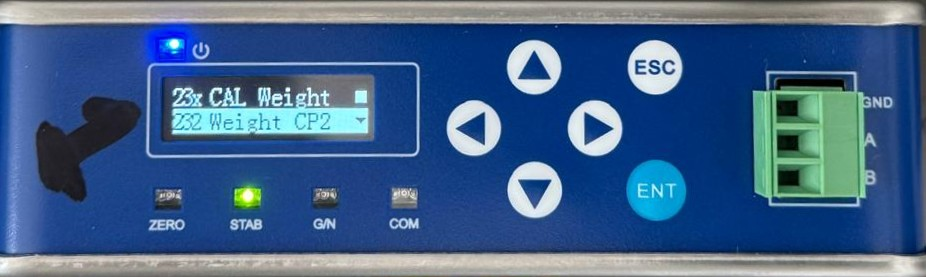
\includegraphics[width=5.72917in,height=\textheight,keepaspectratio]{images/media/98_weight_cp2.jpeg}

  }

  \caption{\textbf{Figure 98.} Selecting 232 Weight CP2.}

  \end{figure}%
\item
  Again, you will see the millivolts as read by the loadcell displayed
  at the top of the screen. At the bottom, it will first show 000.000.
  Put the 5 kg weight on scale 1. Use the right arrow to move the cursor
  to the third 0 and then press the up arrow to adjust it to the weight
  that's on the scale, i.e., 5 kg. \ul{Note the millivolts may be
  slightly different than the picture below.}

  \begin{figure}[H]

  {\centering 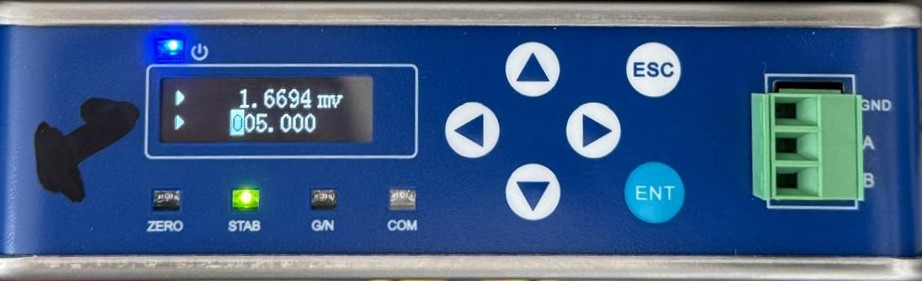
\includegraphics[width=5.72917in,height=\textheight,keepaspectratio]{images/media/99_5kg_millivolts.jpeg}

  }

  \caption{\textbf{Figure 99.} Adjusting the displayed value to 5 kg
  using the arrow keys.}

  \end{figure}%
\item
  As soon as you see the green stable weight (\textbf{STAB}) light come
  on, or note a break in the wind, press Enter (\textbf{ENT}). It should
  now read \textbf{Set Successfully} on the screen (see Figure 93).
\item
  You have now successfully calibrated scale 1 with a 1 kg and 5 kg
  weight. Repeat the above steps with a 6 kg weight (1 kg + 5 kg
  together) following the steps below.
\item
  You should see \textbf{232 Weight CP2} displayed on the screen again
  after you successfully calibrated it in the previous step. Press the
  down arrow once to show \textbf{233 Weight CP3} and press Enter
  (\textbf{ENT}).

  \begin{figure}[H]

  {\centering 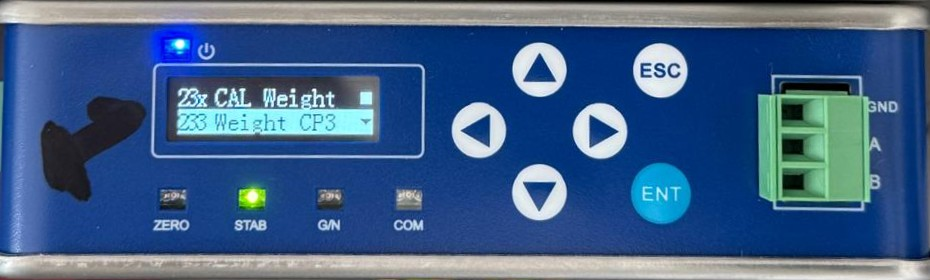
\includegraphics[width=5.72917in,height=\textheight,keepaspectratio]{images/media/100_weight_cp3.jpeg}

  }

  \caption{\textbf{Figure 100.} Selecting 233 Weight CP3.}

  \end{figure}%
\item
  Again, you will see the millivolts as read by the loadcell displayed
  at the top of the screen. At the bottom, it will first show 000.000.
  Put the 1 kg and 5 kg weights together on scale 1. Use the right arrow
  to move the cursor to the third 0 and then press the up arrow to
  adjust it to the weight that's on the scale, i.e., 6 kg. \ul{Note the
  millivolts may be slightly different than the picture below.}

  \begin{figure}[H]

  {\centering 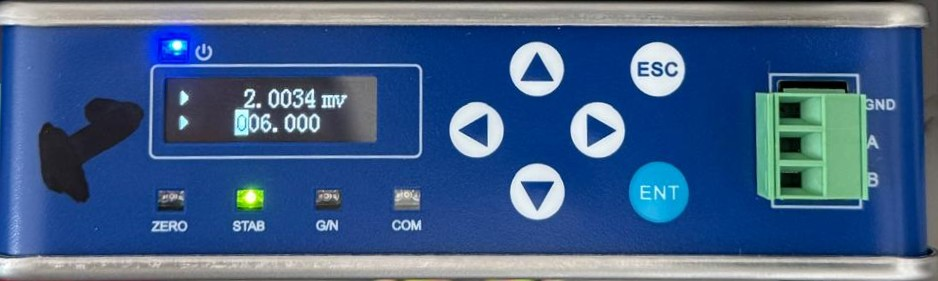
\includegraphics[width=5.72917in,height=\textheight,keepaspectratio]{images/media/101_6kg_millivolts.jpeg}

  }

  \caption{\textbf{Figure 101.} Adjusting the displayed value to 6 kg
  using the arrow keys.}

  \end{figure}%
\item
  As soon as you see the green stable weight (\textbf{STAB}) light come
  on, or note a break in the wind, press Enter (\textbf{ENT}). It should
  now read \textbf{Set Successfully} on the screen (see Figure 93).
\item
  You have now completed all steps for calibrating scale 1 with 1 kg, 5
  kg, and 6 kg. Remove all the weights.
\item
  Press the Escape button (\textbf{ESC}) twice until you get back to the
  main screen displaying just the weight reading. It should now read
  0.000 kg, or be within 5 g of 0.000 kg.
\item
  If scale 1 is within the 5 g threshold, \textbf{repeat the exact same
  steps for scale 2.} Otherwise, repeat the calibration steps again and
  check that the scale reads withing 5 g.
\end{enumerate}

\subsubsection{Record the weight readings after
calibration}\label{record-the-weight-readings-after-calibration}

\begin{itemize}
\item
  Make sure that there are no weights on the scales. Test the accuracy
  of the calibration with no weight, 1 kg, 5 kg, and 6 kg on the scales.
  The scales should be within 5 g of the true weight after calibration.
\item
  Start with scale 1 (colony side). Record the weight reading when no
  weights are on scale 1.
\item
  Place the 1 kg weight on scale 1 and record the reading.
\item
  Place the 5 kg weight on scale 1 and record the reading.
\item
  Place the 6 kg weight (1 kg + 5 kg weights together) on scale 1 and
  record the reading.
\item
  If any of the above readings is out by more than 5 grams, repeat the
  calibration for that particular scale starting with 1 kg, then 5 kg,
  then 6 kg and check again.
\item
  If scale 1 is within the 5 g threshold, \textbf{repeat the exact same
  steps for scale 2.} Otherwise, repeat the calibration steps again and
  check that the scale reads withing 5 g.
\end{itemize}

\subsubsection{Turn on scales scripts and log weight
readings}\label{turn-on-scales-scripts-and-log-weight-readings}

Once you have completed all the steps above to zero and calibrate the
scales, remember to turn on the scales service again to start logging
any penguins that cross the weighbridge, and if you haven't done so
before, log all the weight readings using the log.py script.

\begin{Shaded}
\begin{Highlighting}[]
\FunctionTok{sudo}\NormalTok{ systemctl start scales}
\FunctionTok{sudo}\NormalTok{ systemctl status scales}

\ExtensionTok{python3}\NormalTok{ apms/log.py}
\end{Highlighting}
\end{Shaded}

\begin{tcolorbox}[enhanced jigsaw, left=2mm, toptitle=1mm, breakable, opacitybacktitle=0.6, title=\textcolor{quarto-callout-note-color}{\faInfo}\hspace{0.5em}{Note}, colback=white, opacityback=0, rightrule=.15mm, leftrule=.75mm, colbacktitle=quarto-callout-note-color!10!white, bottomtitle=1mm, titlerule=0mm, coltitle=black, colframe=quarto-callout-note-color-frame, arc=.35mm, bottomrule=.15mm, toprule=.15mm]

\begin{itemize}
\item
  Always follow the exact order: no weight → 1 kg → 5 kg → 6 kg, when
  taking weight readings before, during and after calibrations.
\item
  Place weights gently in the centre of the scale platform and wait for
  the reading to settle before recording it.
\item
  If you have already zeroed (tared) and calibrated the scales and the
  readings are more than 5 grams out, then zero the scales again and
  calibrate again until the reading is as close to accurate as possible.
  A maximum of 5 grams is okay.
\item
  Keep test weights clean and dry --- dirt or moisture can cause the
  weights to corrode and eventually change the physical weight.
\item
  Take care not to drop the weights on the ground (or on the scales) as
  it can damage them and chip away little pieces which will over time
  cause it to be inaccurate.
\end{itemize}

\end{tcolorbox}

\begin{tcolorbox}[enhanced jigsaw, left=2mm, toptitle=1mm, breakable, opacitybacktitle=0.6, title=\textcolor{quarto-callout-tip-color}{\faLightbulb}\hspace{0.5em}{Tip}, colback=white, opacityback=0, rightrule=.15mm, leftrule=.75mm, colbacktitle=quarto-callout-tip-color!10!white, bottomtitle=1mm, titlerule=0mm, coltitle=black, colframe=quarto-callout-tip-color-frame, arc=.35mm, bottomrule=.15mm, toprule=.15mm]

The steps below are done once per scale unless noted otherwise:

\begin{itemize}
\item
  Ensure weight logging is switched off
  \texttt{sudo\ systemctl\ stop\ scales} before recording weight
  readings, taring scales, or calibrating scales..
\item
  Record the BEFORE readings on both scales: no weight, 1 kg, 5 kg, then
  6 kg (1 kg + 5 kg together).
\item
  Clean each scale --- remove sand, sticks, and debris from around and
  under the pan.
\item
  Zero (tare) each scale: \textbf{2xx Weight\&CAL} → \textbf{22x CAL
  Zero} → \textbf{211 Auto Capture}.
\item
  Calibrate each scale:

  \begin{itemize}
  \item
    \textbf{2xx Weight\&CAL} → \textbf{23x CAL Weight} → \textbf{231
    Weight CP1} with 1 kg.
  \item
    \textbf{2xx Weight\&CAL} → \textbf{23x CAL Weight} → \textbf{232
    Weight CP2} with 5 kg.
  \item
    \textbf{2xx Weight\&CAL} → \textbf{23x CAL Weight} → \textbf{233
    Weight CP3} with 6 kg.
  \end{itemize}
\item
  Record the AFTER readings on each scale (no weight, 1 kg, 5 kg, 6 kg).
  If any readings are out by more than 5 g, repeat the calibration for
  that scale and check again.
\item
  Finish up: start the scales again
  \texttt{sudo\ systemctl\ start\ scales} and log all the weight
  readings \texttt{python3\ apms/log.py}.
\end{itemize}

\end{tcolorbox}

\subsection{Laumas TLB485 Indicators}\label{laumas-tlb485-indicators}

To check if the system needs to be calibrated, place a 1kg, 5kg and 6kg
(5+1) weight on each scale and observe the readings on the scale
indicators. If the reading is out by more than 5g, recalibrate. The wind
can have a huge influence on the scales and thus \ul{only calibrate on
good weather days}.

There are 4 buttons on each indicator. They are:

\begin{longtable}[]{@{}ll@{}}
\toprule\noalign{}
\endhead
\bottomrule\noalign{}
\endlastfoot
\textbf{ENTER} &

\includegraphics[width=\linewidth,height=0.22in,keepaspectratio]{images/media/image85.png} \\
\textbf{LEFT} &

\includegraphics[width=\linewidth,height=0.22in,keepaspectratio]{images/media/image86.png} \\
\textbf{UP} &

\includegraphics[width=\linewidth,height=0.22in,keepaspectratio]{images/media/image87.png} \\
\textbf{CANCEL/BACK} &

\includegraphics[width=\linewidth,height=0.22in,keepaspectratio]{images/media/image84.png} \\
\end{longtable}

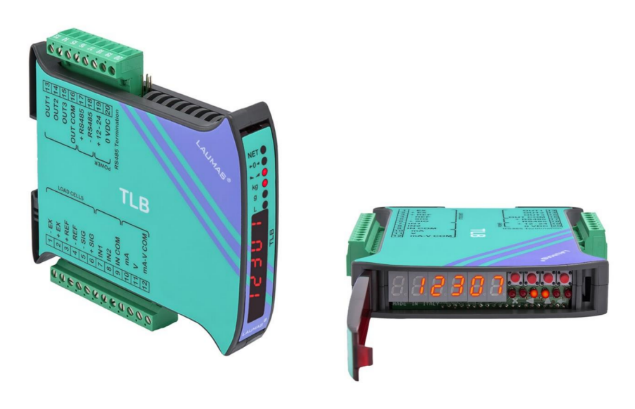
\includegraphics[width=\linewidth,height=1.85in,keepaspectratio]{images/media/image83.png}

\begin{itemize}
\item
  SSH into the Pi
\item
  Stop the scales process: ~~~~~~~~
\end{itemize}

\begin{Shaded}
\begin{Highlighting}[]
\FunctionTok{sudo}\NormalTok{ systemctl stop scales}
\end{Highlighting}
\end{Shaded}

\begin{itemize}
\tightlist
\item
  Log the start of the calibration event: ~~~~
\end{itemize}

\begin{Shaded}
\begin{Highlighting}[]
\ExtensionTok{python3}\NormalTok{ \textasciitilde{}/apms/log.py}
\end{Highlighting}
\end{Shaded}

\begin{itemize}
\tightlist
\item
  Log the weight discrepancy for each scale using the 5kg weight.
\item
  You can run the code below to check that the scripts have indeed
  stopped:
\end{itemize}

\begin{Shaded}
\begin{Highlighting}[]
\ExtensionTok{systemctl}\NormalTok{ status scales}
\ExtensionTok{systemctl}\NormalTok{ status rfid}
\end{Highlighting}
\end{Shaded}

\begin{itemize}
\item
  Remove all weights from scales.
\item
  Tare the scale:

  \begin{itemize}
  \tightlist
  \item
    Hold in the CANCEL button until it displays:
    
\includegraphics[width=\linewidth,height=0.22in,keepaspectratio]{images/media/image158.png}
    Then press ENTER
  \item
    All the Lights should be flashing. Press ENTER again to zero the
    scale.
  \item
    The weight should read 0. Press CANCEL until you are back at the
    main weight display.
  \end{itemize}
\item
  Start with Scale 1 (colony side) and then do Scale 2 (ocean side).
  Start by placing the 5kg weight in the center of the scale. Then
  proceed to the indicator, and flip open the cover to reveal the
  buttons as described above (you might need a small flat screwdriver to
  lift the cover). It can be difficult to see the LED display without
  looking through the cover, so flip it down to confirm what is
  displayed if uncertain.
\item
  While pressing and holding the ENTER button, also press the CANCEL
  button. This should display
  
\includegraphics[width=\linewidth,height=0.22in,keepaspectratio]{images/media/image159.png}
\item
  Press ENTER. Now use
  
\includegraphics[width=\linewidth,height=0.22in,keepaspectratio]{images/media/image162.png}
  to select
  
\includegraphics[width=\linewidth,height=0.22in,keepaspectratio]{images/media/image160.png}
  and press ENTER
\item
  A flashing weight should be displayed. All the lights should be OFF
\item
  Use
  
\includegraphics[width=\linewidth,height=0.22in,keepaspectratio]{images/media/image162.png}
  to adjust the weight until it reads exactly 5.000 kg

  
\includegraphics[width=\linewidth,height=0.22in,keepaspectratio]{images/media/image86.png}
  to change value

  
\includegraphics[width=\linewidth,height=0.22in,keepaspectratio]{images/media/image87.png}
  to change decimal place holder
\item
  Press ENTER. The new weight should be displayed, and all the lights
  should be flashing.
\item
  Press ENTER one more time. This should show again. Press CANCEL until
  you see the weight displayed.
\item
  Check with 1kg, 5kg and 6kg weights again. It should be within 1g. If
  not, recalibrate.
\item
  Start the APMS processes.
\end{itemize}

\begin{Shaded}
\begin{Highlighting}[]
\FunctionTok{sudo}\NormalTok{ systemctl start scales}
\FunctionTok{sudo}\NormalTok{ systemctl start rfid}
\end{Highlighting}
\end{Shaded}

\begin{itemize}
\tightlist
\item
  Log the end of the calibration event: ~~~~
\end{itemize}

\begin{Shaded}
\begin{Highlighting}[]
\ExtensionTok{python3}\NormalTok{ \textasciitilde{}/apms/log.py}
\end{Highlighting}
\end{Shaded}

\section{Troubleshooting}\label{troubleshooting}

There are too many permutations of how things can go wrong to cover it
all in this manual. However, some common things to look out for, as well
as how to go about getting more information, will be discussed below.

Often, the dashboard will give an indication of something going wrong. A
classic example of this would be seeing the solar supply voltage going
down and the batteries not fully charging. This is often due to
overgrowth and the dashboard should be checked the next day to see if it
has improved. The dashboard could also show the system being healthy,
but the algorithm shows something is wrong, such as the number of RFID
tags dropping to zero for a few days. This could be due to the BioMark
system failing, or the RFID antenna shifting out of position.

For diagnosing problems, or just checking in on the system, the Monitor
can be used.

If the Monitor has power, it should operate and be able to give
information about the system, even if the Main Unit is completely dead.
Ensure the SIM card has airtime to be able to reply via SMS.

\begin{itemize}
\item
  The Monitor will send a SMS to the operator in the event of the
  following:

  \begin{itemize}
  \item
    If the 4V of the SIM800L is too low/high (only v1.1 of the APMS,
    v1.2 no longer uses the 4V SIM module)
  \item
    If the 5V of the Raspberry Pi is too low/high
  \item
    If the 12V of the scales/router is too low/high
  \item
    If the 24V solar supply is too low/high
  \item
    If the ambient temperature is too high. (Warning: 50°C - Danger at
    60°C)
  \item
    If the Raspberry Pi or Monitor reboot
  \end{itemize}
\end{itemize}

If any of these messages are received, the operator should investigate.

\subsection{Monitor Commands}\label{monitor-commands}

A simple set of commands can be used by the administrator to diagnose
system faults via SMS.

To send a command to the Monitor, send a SMS starting with
\textbf{``CMD:''}

For example, to request a status report, send:

\begin{Shaded}
\begin{Highlighting}[]
\ExtensionTok{CMD:S}
\end{Highlighting}
\end{Shaded}

The monitor should reply, via SMS, with a brief status report. The
status report is discussed in ***

Note the commands are not case sensitive.

The table below shows a list of valid commands.

\begin{longtable}[]{@{}
  >{\raggedright\arraybackslash}p{(\linewidth - 4\tabcolsep) * \real{0.2639}}
  >{\raggedright\arraybackslash}p{(\linewidth - 4\tabcolsep) * \real{0.2222}}
  >{\raggedright\arraybackslash}p{(\linewidth - 4\tabcolsep) * \real{0.5000}}@{}}
\toprule\noalign{}
\begin{minipage}[b]{\linewidth}\raggedright
\textbf{Command Name}
\end{minipage} & \begin{minipage}[b]{\linewidth}\raggedright
\textbf{What to send}
\end{minipage} & \begin{minipage}[b]{\linewidth}\raggedright
\textbf{Description}
\end{minipage} \\
\midrule\noalign{}
\endhead
\bottomrule\noalign{}
\endlastfoot
Request Status Report & CMD:S & The Monitor should reply by sending a
status report via SMS \\
Reboot & CMD:R & This power cycles the Raspberry Pi \\
Power On/Off & CMD:P & This powers the Raspberry Pi on if it was off,
and off if it was on \\
Update Time & CMD:U & This updates the Monitor system time. \\
Change Phone Number of Operator &
\begin{minipage}[t]{\linewidth}\raggedright
CMD:M+27**\\
*******\strut
\end{minipage} & This changes the phone number of the operator, saved in
the non-volatile memory of the Monitor. \\
Turn Off SMS Notifications & CMD:X & To turn off SMS notifications from
the Monitor. \\
Turn On SMS Notifications & CMD:Y & To turn on SMS notifications from
the Monitor \\
Send BASH command & CM D:C***** & UNTESTED

Send a BASH Command for the Pi to execute next time it checks in. \\
\end{longtable}

\subsection{Status Report (CMD:S)}\label{status-report-cmds}

An example of a status report as received from the Stony Point Monitor
can be seen below. The example will be used to explain the different
parameters.

\begin{figure}[H]

{\centering 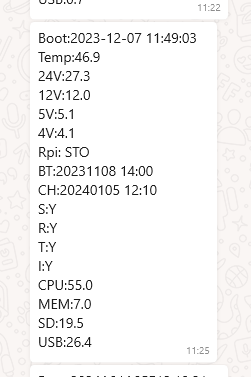
\includegraphics[width=6.25in,height=\textheight,keepaspectratio]{images/media/88_status.png}

}

\caption{\textbf{Figure 88.} Status report sent via the APMS's SIM
module.}

\end{figure}%

\chapter{Checking the System for
Accuracy}\label{checking-the-system-for-accuracy}

To know whether an APMS is functioning properly and providing accurate
data, a cross check is performed. This is done by using a third,
independent scale. The scale is powered from its own batteries and must
be calibrated on site. This is explained in the manual that was supplied
with the scale. A camera is placed to have a clear view of the weight
readout on the LCD screen. The camera should also be positioned to have
all three scales in view. The penguins do occasionally stand still on
the independent scale. When this happens, the weight reading will not
fluctuate a clear weight can be read and recorded. All the known weights
should be identified and then compared with what the algorithm produced.
The scale currently being used is accurate to the nearest 5g.

\section{Testing and Calibration of
System}\label{testing-and-calibration-of-system}

To test the accuracy of the APMS weighbridge, the weight estimates are
compared to that obtained by an independent scale. Video footage is
captured of the two main scales, as well as the independent scale. The
independent scale has an LCD display, and this should be visible to the
camera. It does have a night light and should thus be hidden as much as
possible from view, as the penguins are very aware of changes to their
surroundings and get easily frazzled. The video clips showing penguins
stationary on the independent scale will be used to find the ``true''
weight, while the footage of the main two scales will be used to
characterise the data. The penguin should be stationary on the
independent scale, long enough to confidently read a stable reading from
the LCD display.

\url{_book/videos/16_testing_calibrations.mp4}

You will need the following

\begin{enumerate}
\def\labelenumi{\arabic{enumi}.}
\item
  A laptop with WiFi. (Take a LAN cable with just in case)
\item
  Certified 1kg and 5kg weights
\item
  Independent scale with fresh batteries and canvas cover.
\item
  Camera to capture footage. Currently using the Reolink Go Ranger.
  Ensure it is charged and that you have the solar panel + zip ties
\item
  In addition to this, always take a basic tool kit and power supply
  with, as you never know what you might find at the site.
\end{enumerate}

\subsection{To perform the
testing/calibration}\label{to-perform-the-testingcalibration}

\begin{enumerate}
\def\labelenumi{\arabic{enumi}.}
\item
  Choose good weather and observe when the best time is to set up
  (usually mid day is good when less penguins cross the weighbridge).
\item
  SSH into the system and log the start of the testing/calibration event
  in the log file:
\end{enumerate}

\begin{Shaded}
\begin{Highlighting}[]
\ExtensionTok{python3}\NormalTok{ apms/log.py}
\end{Highlighting}
\end{Shaded}

\begin{enumerate}
\def\labelenumi{\arabic{enumi}.}
\setcounter{enumi}{2}
\item
  The independent scale must be set up as described in the section
  above.
\item
  Calibrate the scales as described in the section
  \hyperref[Routineux5cux2520Calibrationux5cux2520ofux5cux2520Scales]{Routine
  Calibration of Scales}
\item
  Ensure the camera has a clear view of the 2 main scales, the
  independent scale, and the LCD display
\item
  After at least one day of capturing footage, SSH back into the system
  and log the end of the event in the log file.
\item
  Remove the camera and independent scale, leaving the site as
  undisturbed as possible.
\item
  The data can then be manually processed or the user can wait for the
  daily file which is automatically generated by the algorithm at 2AM
  every morning.
\item
  Compare the weights obtained from the footage with the weights
  generated by the algorithm
\item
  If the penguin weight is out by more than 50g, adjust the following
  parameters and run the algorithm manually to check again.

  \begin{enumerate}
  \def\labelenumii{\alph{enumii}.}
  \item
    \texttt{MAX\_PENGUIN\_WEIGHT} - The maximum weight of a penguin
    expected to walk over the scales.
  \item
    \texttt{MIN\_PENGUIN\_WEIGHT} - The minimum weight of a penguin
    expected to walk over the scales.
  \item
    \texttt{MAX\_SCALES\_DIFFERENCE\_ALLOWED} - Difference allowed
    between weight measured on Scale 1 and Scale 2.
  \item
    \texttt{CLIMB\_ON\_DURATION\_MIN} - Minimum amount of time it takes
    a penguin to climb on.
  \end{enumerate}
\end{enumerate}

\subsection{Setup Procedure for Independent
Scale}\label{setup-procedure-for-independent-scale}

\begin{enumerate}
\def\labelenumi{\arabic{enumi}.}
\item
  Ensure scale has fresh batteries.
\item
  Ensure the scale has the canvas cover on.
\item
  Put the scale on a flat surface and ensure the scale is level.
\item
  Test with 1kg, 5kg and 6kg weight. It should be spot on.

  \begin{enumerate}
  \def\labelenumii{\alph{enumii}.}
  \item
    Calibrate according to the user manual, if required
  \item
    Please see the manual for the specific scale you are using. The
    independent scale we are currently using is the Adam CPW Plus-15
    scale. \href{./_book/files/CPWplus_UM_USA.pdf}{Download the manual
    here.}
  \end{enumerate}
\item
  At the site, also ensure the scale is level, and recheck with weights.
\item
  Place the display as far away and out of sight from the penguins as
  possible.
\end{enumerate}

\chapter{Conclusion}\label{conclusion}

The system was built as a platform for future expansions and
experiments. There are GPIO ports available on the Raspberry Pi, the CPU
has the capacity to do more work and the Monitor can be programmed with
more features. The data processing algorithm is also a first attempt and
the raw data can be processed differently in future if desired.


\backmatter


\end{document}
